\documentclass{article}

\usepackage{graphicx} % Required for inserting images
\usepackage[left=1in,right=1in,top=1in,bottom=1in]{geometry} \usepackage{amsmath}
\usepackage{amsthm} %proof environment
\usepackage{amsthm} %proof environment
\usepackage{amssymb}
\usepackage{amsfonts}
\usepackage{enumitem} %nice lists
\usepackage{verbatim} %useful for something 
\usepackage{xcolor}
\usepackage{setspace}
\usepackage{titlesec}
\usepackage{blindtext} % I have no idea what this is 
\usepackage{caption}  % need this for unnumbered captions/figures
\usepackage{natbib}
\usepackage{appendix}
\usepackage{tikz}
\usepackage{hyperref}


\hypersetup{
    colorlinks=true,
    linkcolor=blue,
    filecolor=magenta,      
    urlcolor=blue,
    pdftitle={Overleaf Example},
    pdfpagemode=FullScreen,
    }

\titleformat{\section}{\bfseries\Large}{Problem \thesection:}{5pt}{}

\begin{document}

\title{AM 260 - Computational Fluid Dynamics: Homework 4}
\author{Dante Buhl}


\newcommand{\wrms}{w_{\text{rms}}}
\newcommand{\bs}[1]{\boldsymbol{#1}}
\newcommand{\tb}[1]{\textbf{#1}}
\newcommand{\bmp}[1]{\begin{minipage}{#1\textwidth}}
\newcommand{\emp}{\end{minipage}}
\newcommand{\R}{\mathbb{R}}
\newcommand{\C}{\mathbb{C}}
\newcommand{\N}{\mathcal{N}}
%\newcommand{\K}{\bs{\mathrm{K}}}
\newcommand{\m}{\bs{\mu}_*}
\newcommand{\s}{\bs{\Sigma}_*}
\newcommand{\dt}{\Delta t}
\newcommand{\dx}{\Delta x}
\newcommand{\tr}[1]{\text{Tr}(#1)}
\newcommand{\Tr}[1]{\text{Tr}(#1)}
\newcommand{\Div}{\nabla \cdot}
\renewcommand{\div}{\nabla \cdot}
\newcommand{\Curl}{\nabla \times}
\newcommand{\Grad}{\nabla}
\newcommand{\grad}{\nabla}
\newcommand{\grads}{\nabla_s}
\newcommand{\gradf}{\nabla_f}
\newcommand{\xs}{x_s}
\newcommand{\x}{\bs{x}}
\newcommand{\xf}{x_f}
\newcommand{\ts}{t_s}
\newcommand{\tf}{t_f}
\newcommand{\pt}{\partial t}
\newcommand{\pz}{\partial z}
\newcommand{\uvec}{\bs{u}}
\newcommand{\bvec}{\bs{B}}
\newcommand{\nvec}{\hat{\bs{n}}}
\newcommand{\tu}{\tilde{\uvec}}
\newcommand{\B}{\bs{B}}
\newcommand{\A}{\bs{A}}
\newcommand{\jvec}{\bs{j}}
\newcommand{\F}{\bs{F}}
\newcommand{\T}{\tilde{T}}
\newcommand{\ez}{\bs{e}_z}
\newcommand{\ex}{\bs{e}_x}
\newcommand{\ey}{\bs{e}_y}
\newcommand{\eo}{\bs{e}_{\bs{\Omega}}}
\newcommand{\ppt}[1]{\frac{\partial #1}{\partial t}}
\newcommand{\pp}[2]{\frac{\partial #1}{\partial #2}}
\newcommand{\pptwo}[2]{\frac{\partial^2 #1}{\partial #2^2}}
\newcommand{\ddtwo}[2]{\frac{d^2 #1}{d #2^2}}
\newcommand{\DDt}[1]{\frac{D #1}{D t}}
\newcommand{\ppts}[1]{\frac{\partial #1}{\partial t_s}}
\newcommand{\pptf}[1]{\frac{\partial #1}{\partial t_f}}
\newcommand{\ppz}[1]{\frac{\partial #1}{\partial z}}
\newcommand{\ddz}[1]{\frac{d #1}{d z}}
\newcommand{\ppzetas}[1]{\frac{\partial^2 #1}{\partial \zeta^2}}
\newcommand{\ppzs}[1]{\frac{\partial #1}{\partial z_s}}
\newcommand{\ppzf}[1]{\frac{\partial #1}{\partial z_f}}
\newcommand{\ppx}[1]{\frac{\partial #1}{\partial x}}
\newcommand{\ddx}[1]{\frac{d #1}{d x}}
\newcommand{\ppxi}[1]{\frac{\partial #1}{\partial x_i}}
\newcommand{\ppxj}[1]{\frac{\partial #1}{\partial x_j}}
\newcommand{\ppy}[1]{\frac{\partial #1}{\partial y}}
\newcommand{\ppzeta}[1]{\frac{\partial #1}{\partial \zeta}}
\renewcommand{\k}{\bs{k}}
\newcommand{\real}[1]{\text{Re}\left[#1\right]}


\maketitle 
% This line removes the automatic indentation on new paragraphs
\setlength{\parindent}{0pt}

\section{Part A}

I have ran all 11 initial conditions using each of the 7 different integration
schemes, and have saved, and plotted all of them. Only the FOG and 3 TVD slope
limiter methods are shown in Figures \ref{fig:sol_1_6} and \ref{fig:sol_7_11}.

\begin{figure}[t]
    \bmp{0.25}
        \centering
        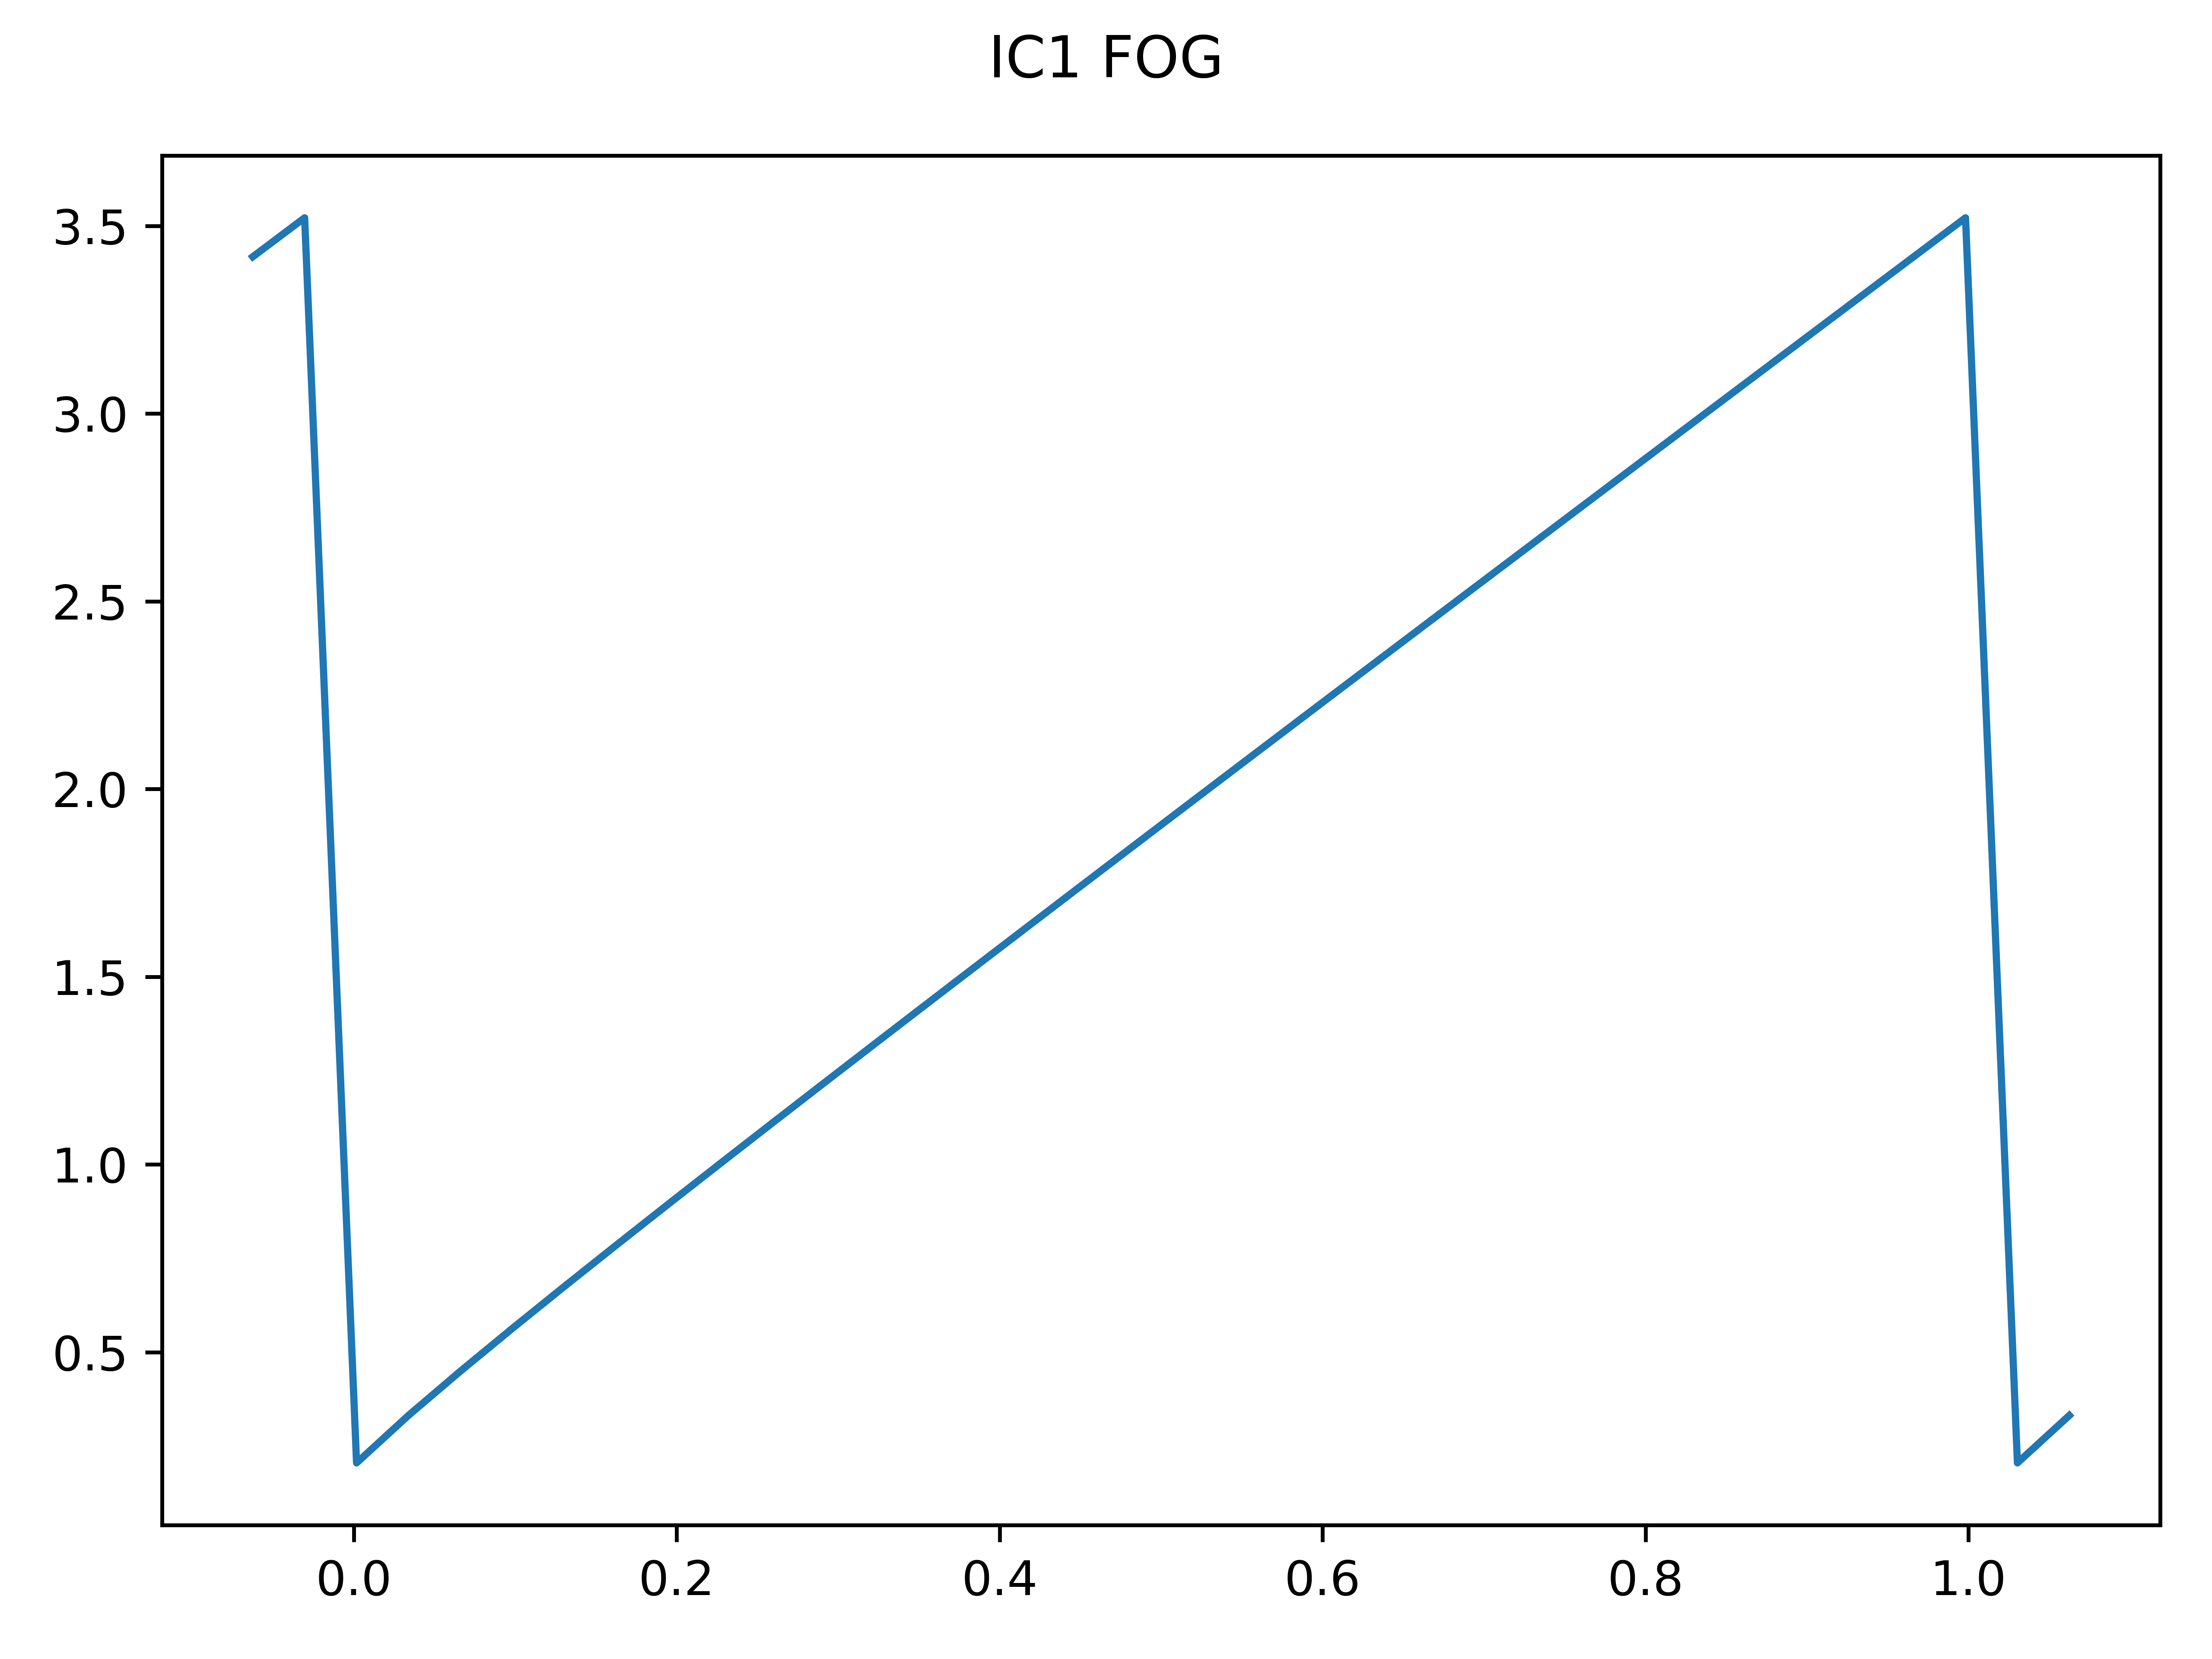
\includegraphics[width=.95\textwidth]{../../code/IC1Methodfu_plot.png}
        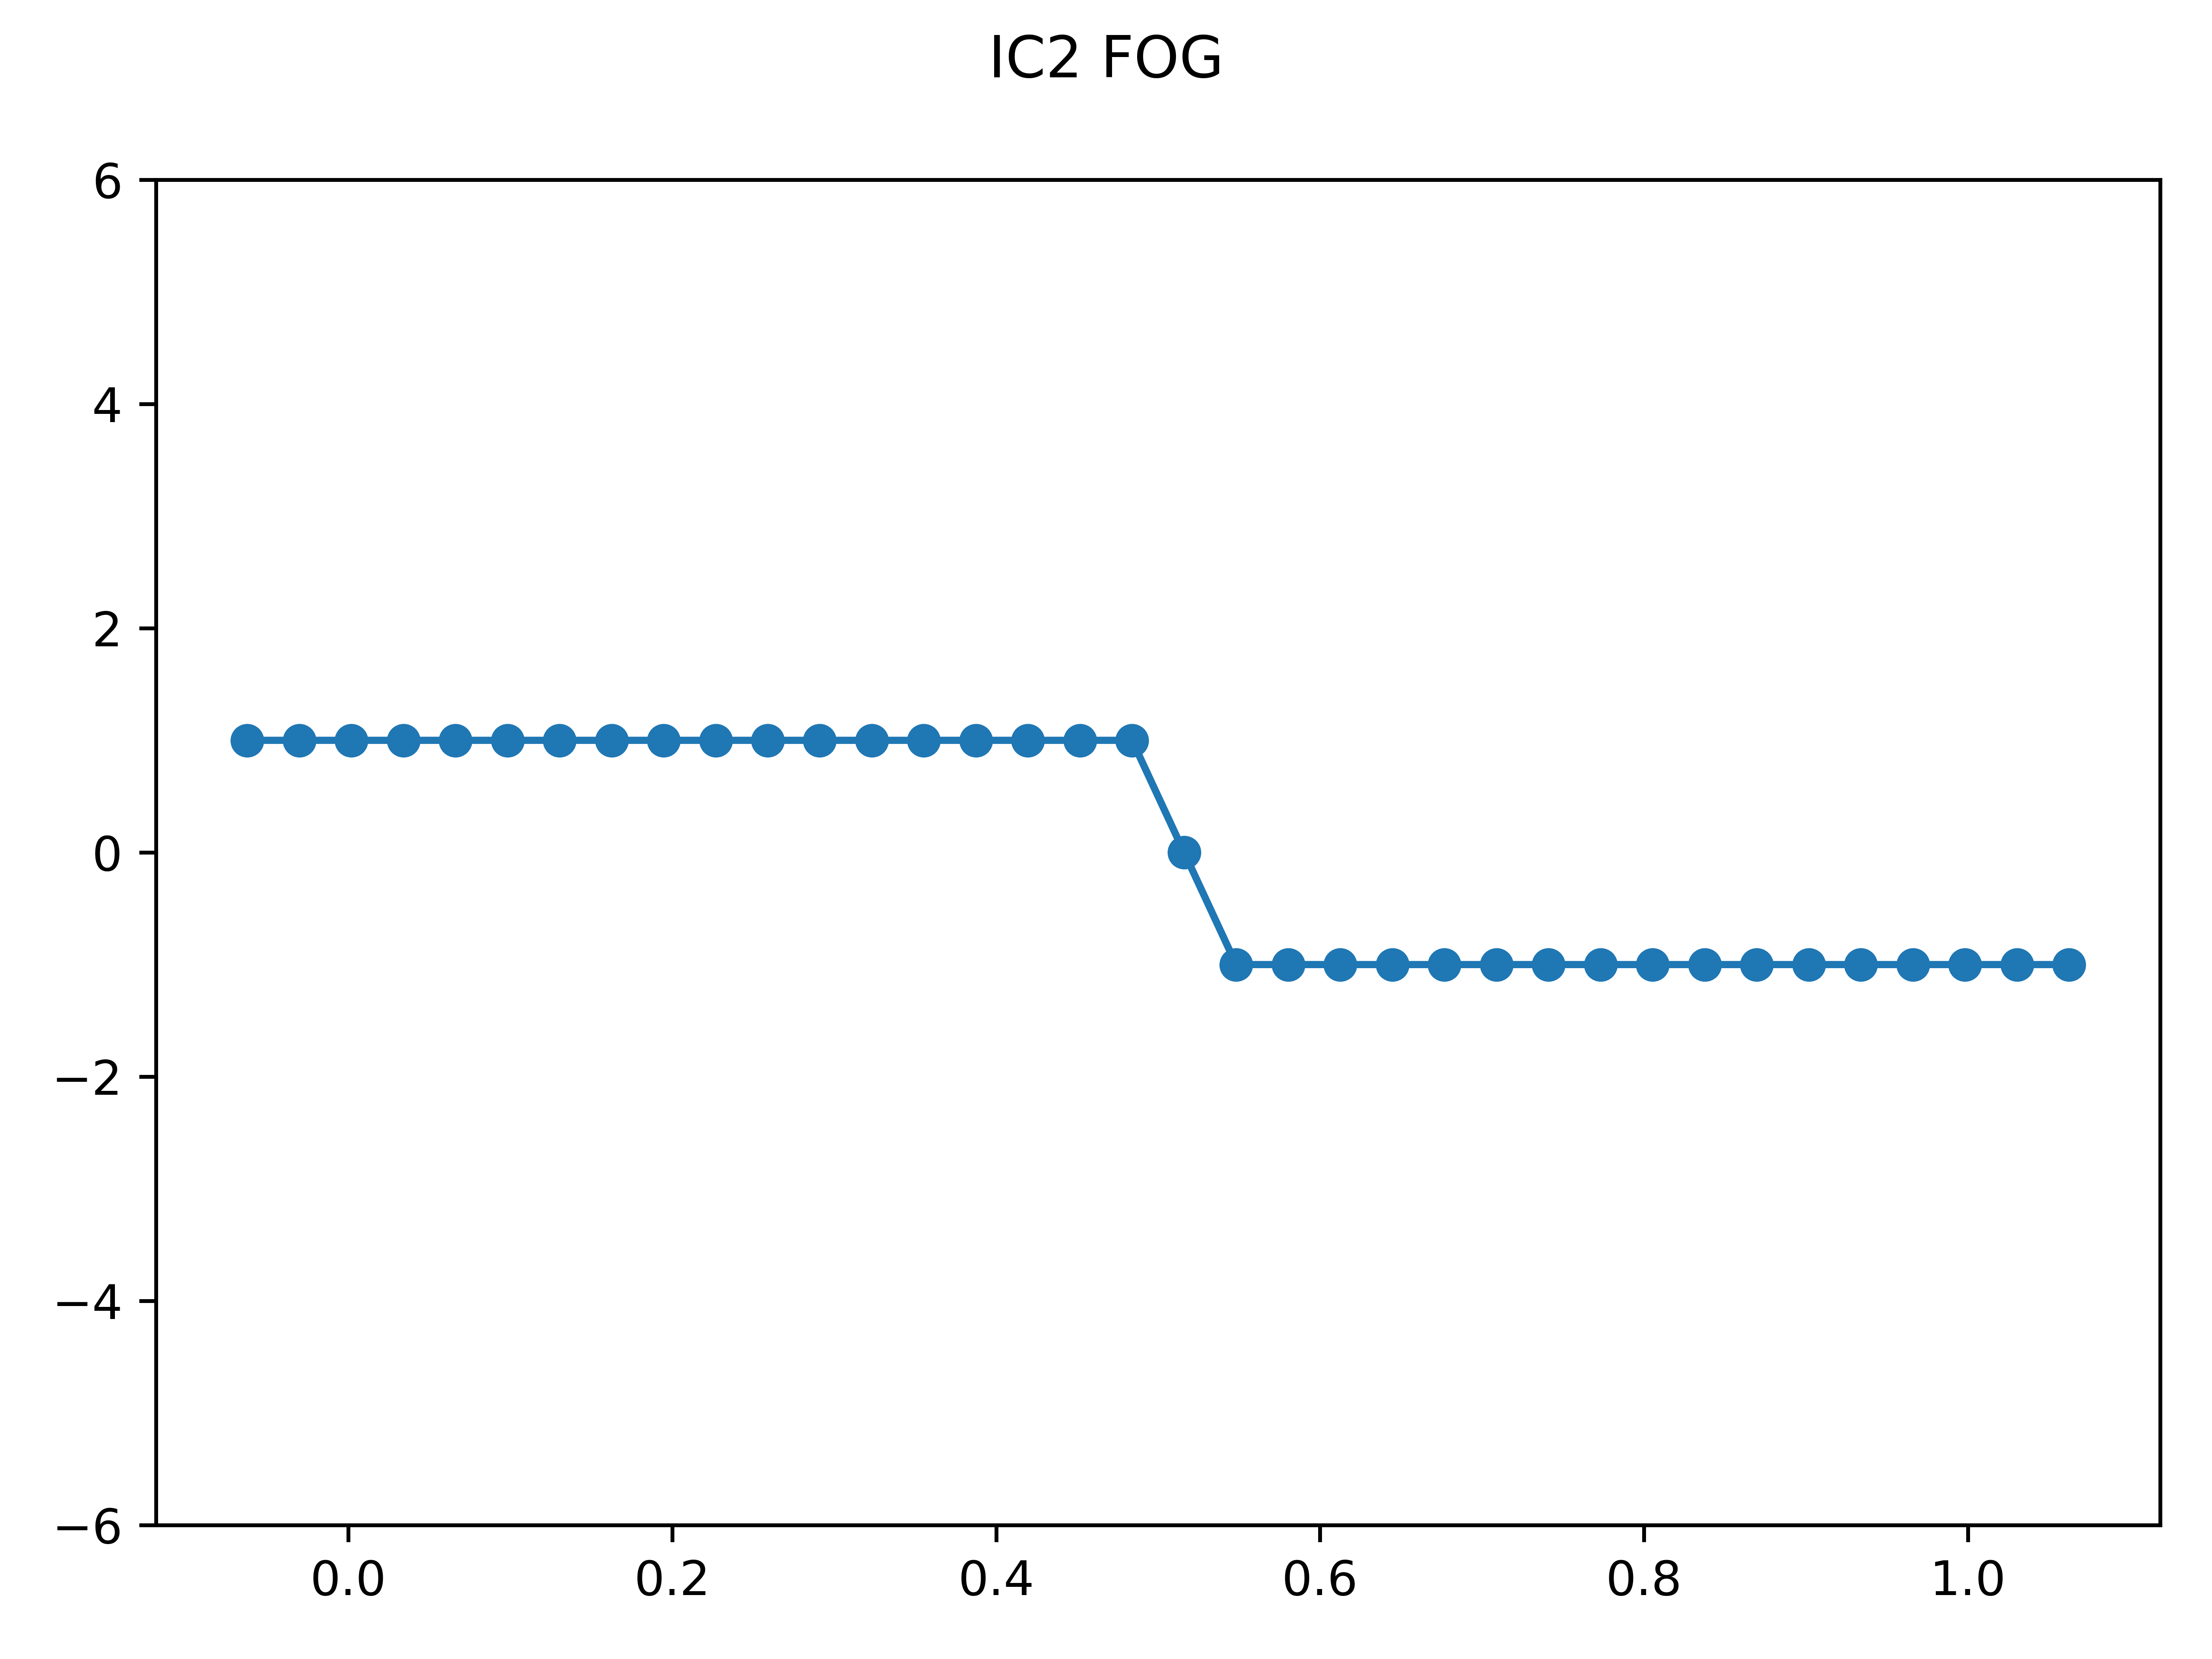
\includegraphics[width=.95\textwidth]{../../code/IC2Methodfu_plot.png}
        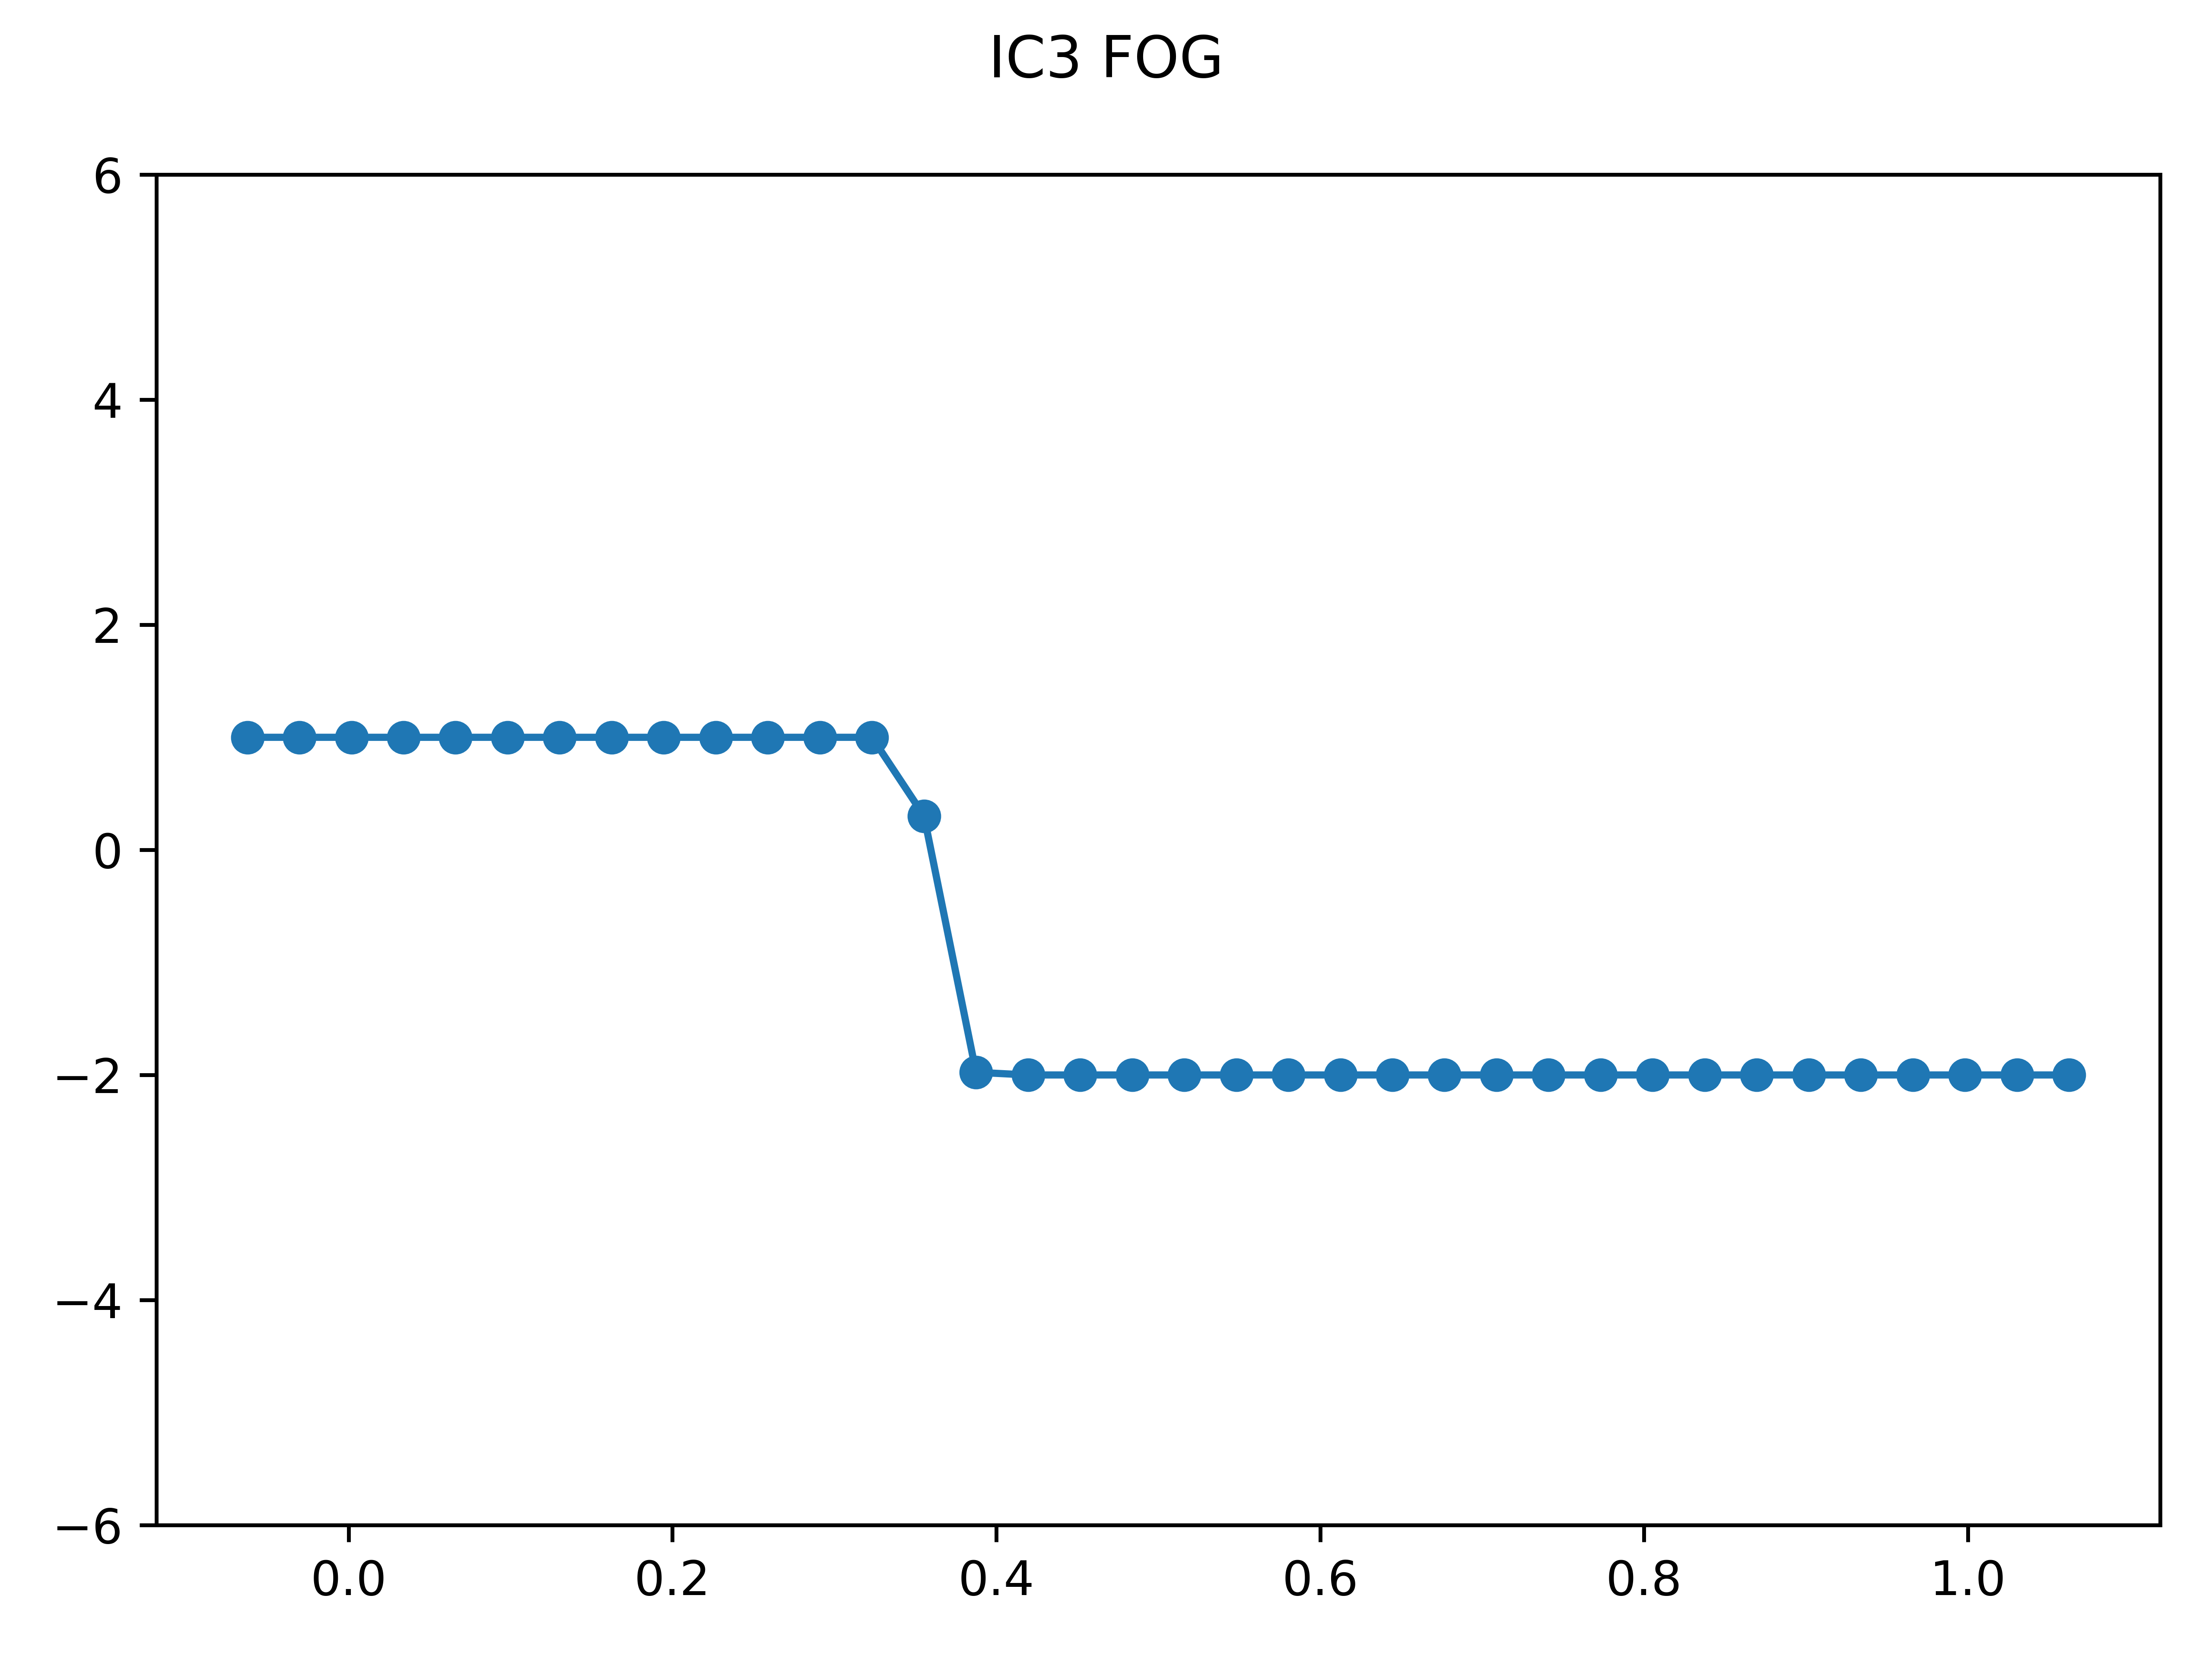
\includegraphics[width=.95\textwidth]{../../code/IC3Methodfu_plot.png}
        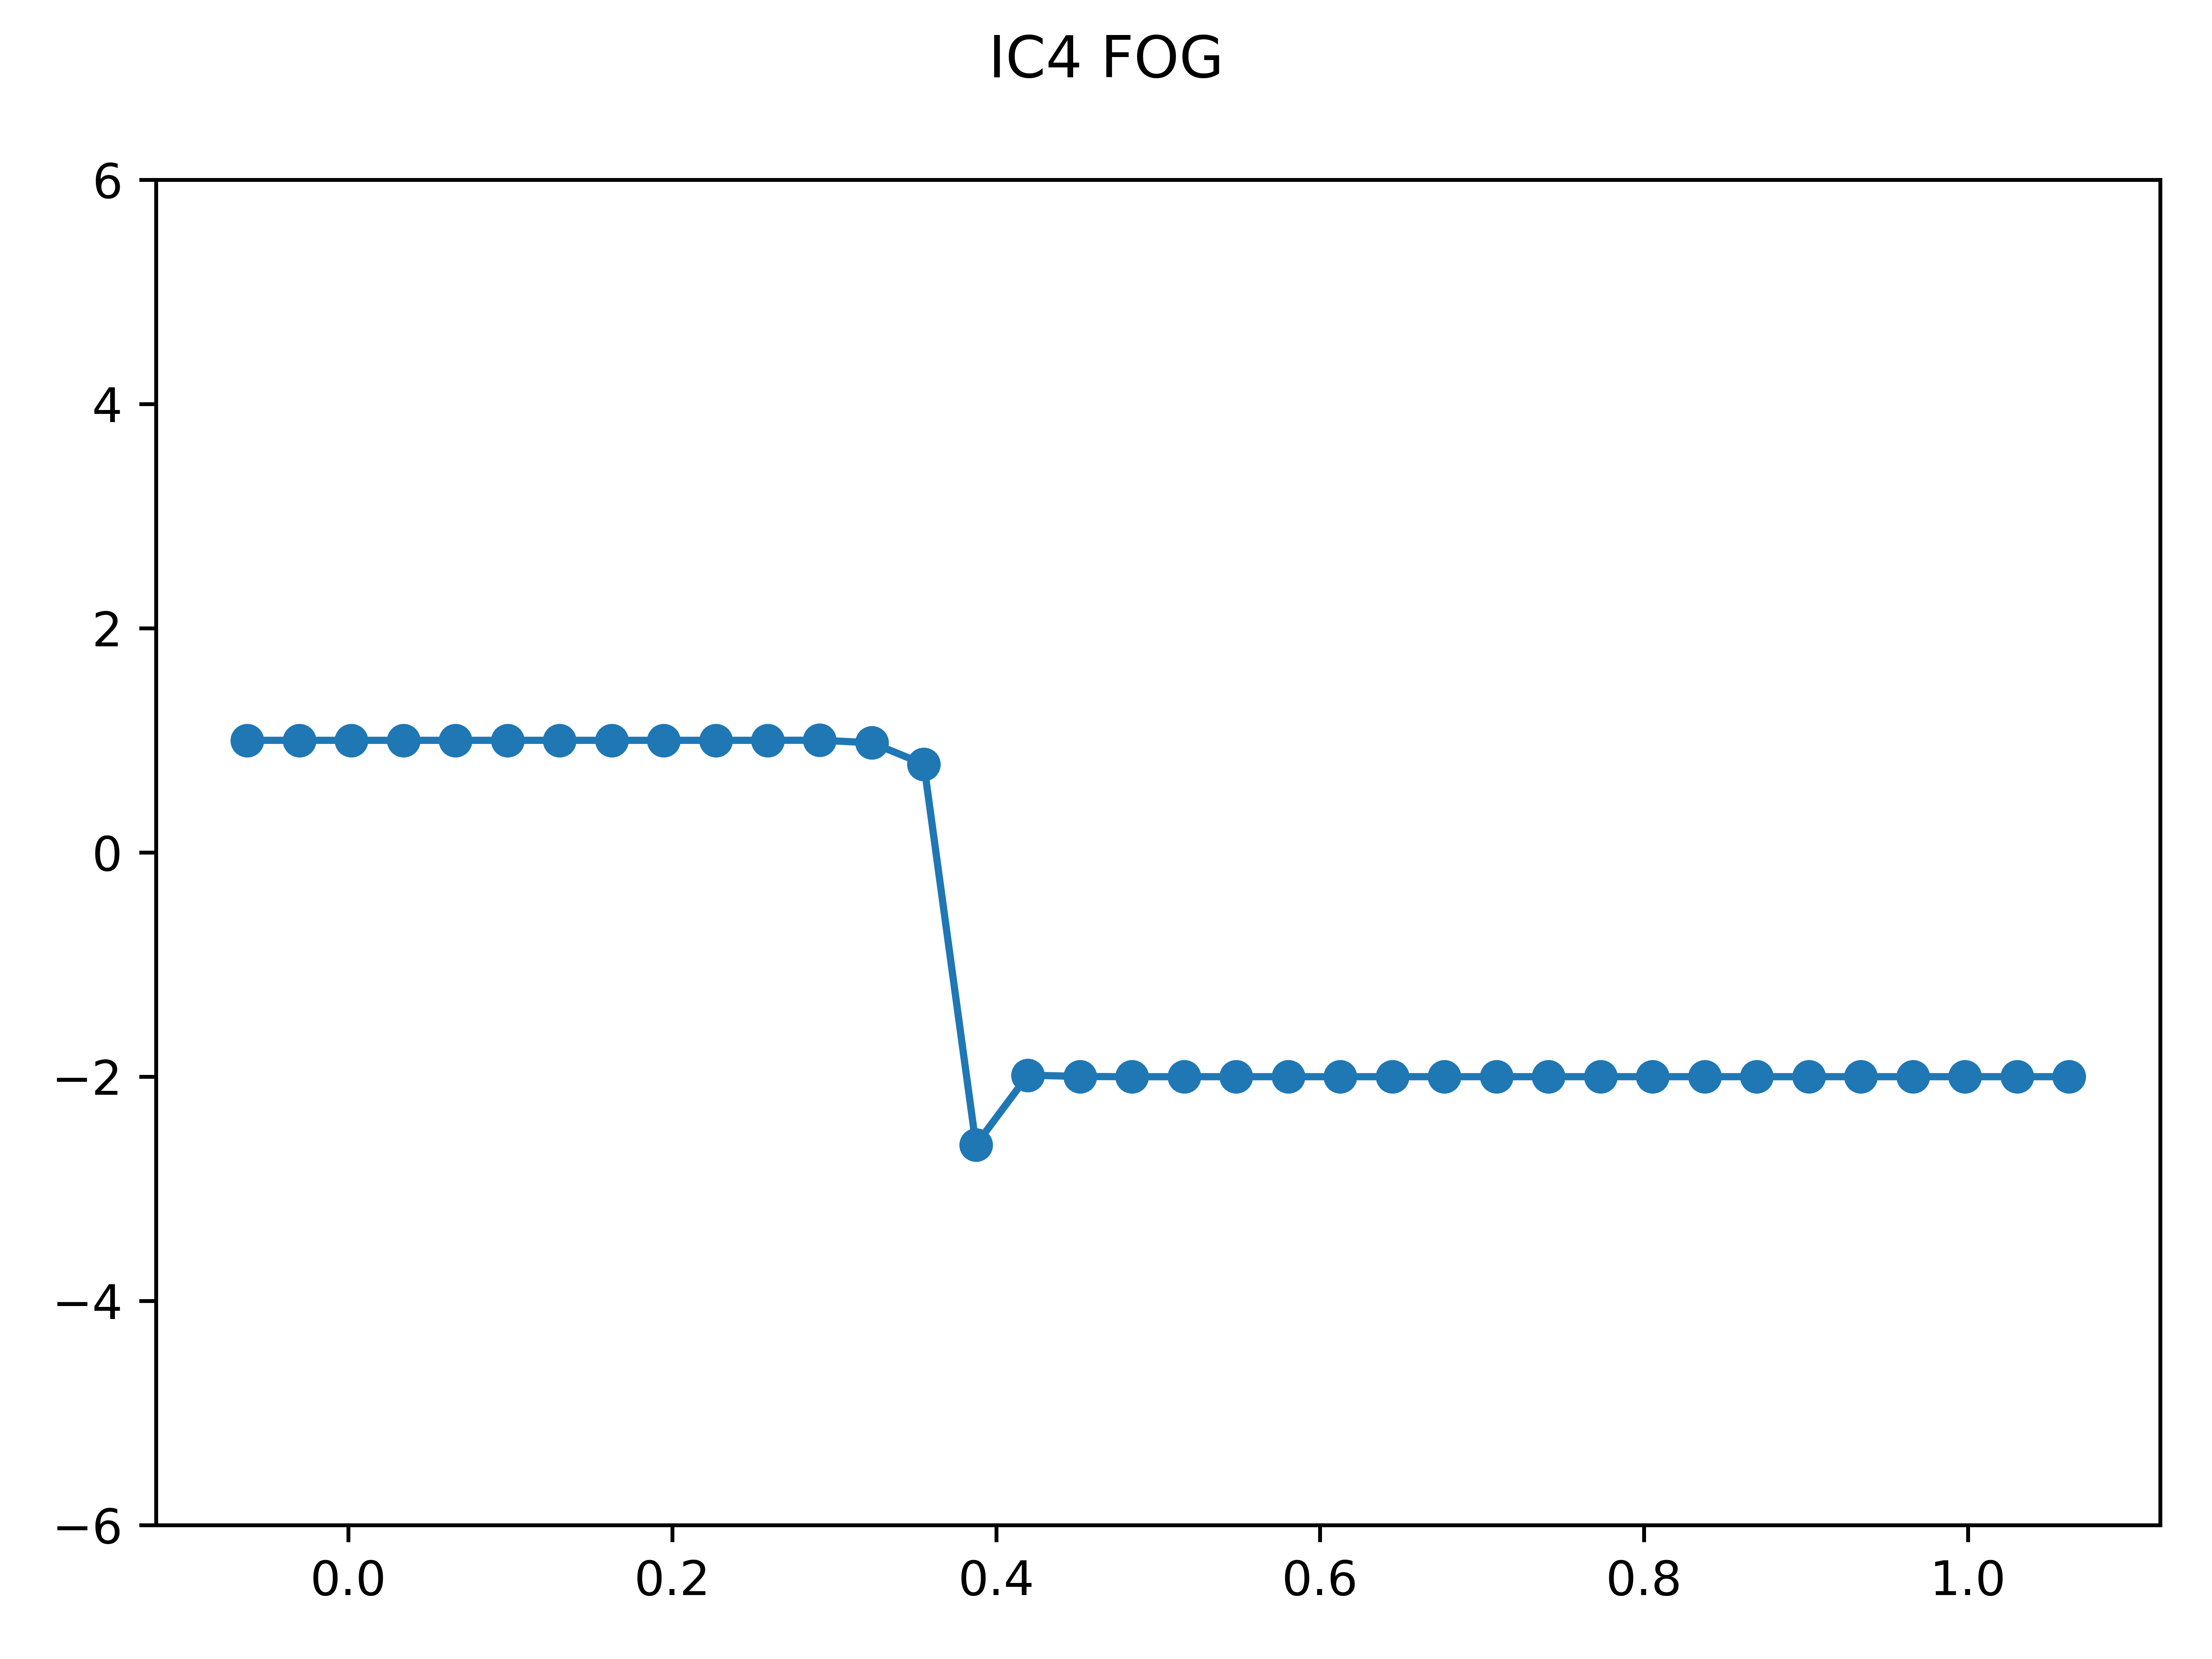
\includegraphics[width=.95\textwidth]{../../code/IC4Methodfu_plot.png}
        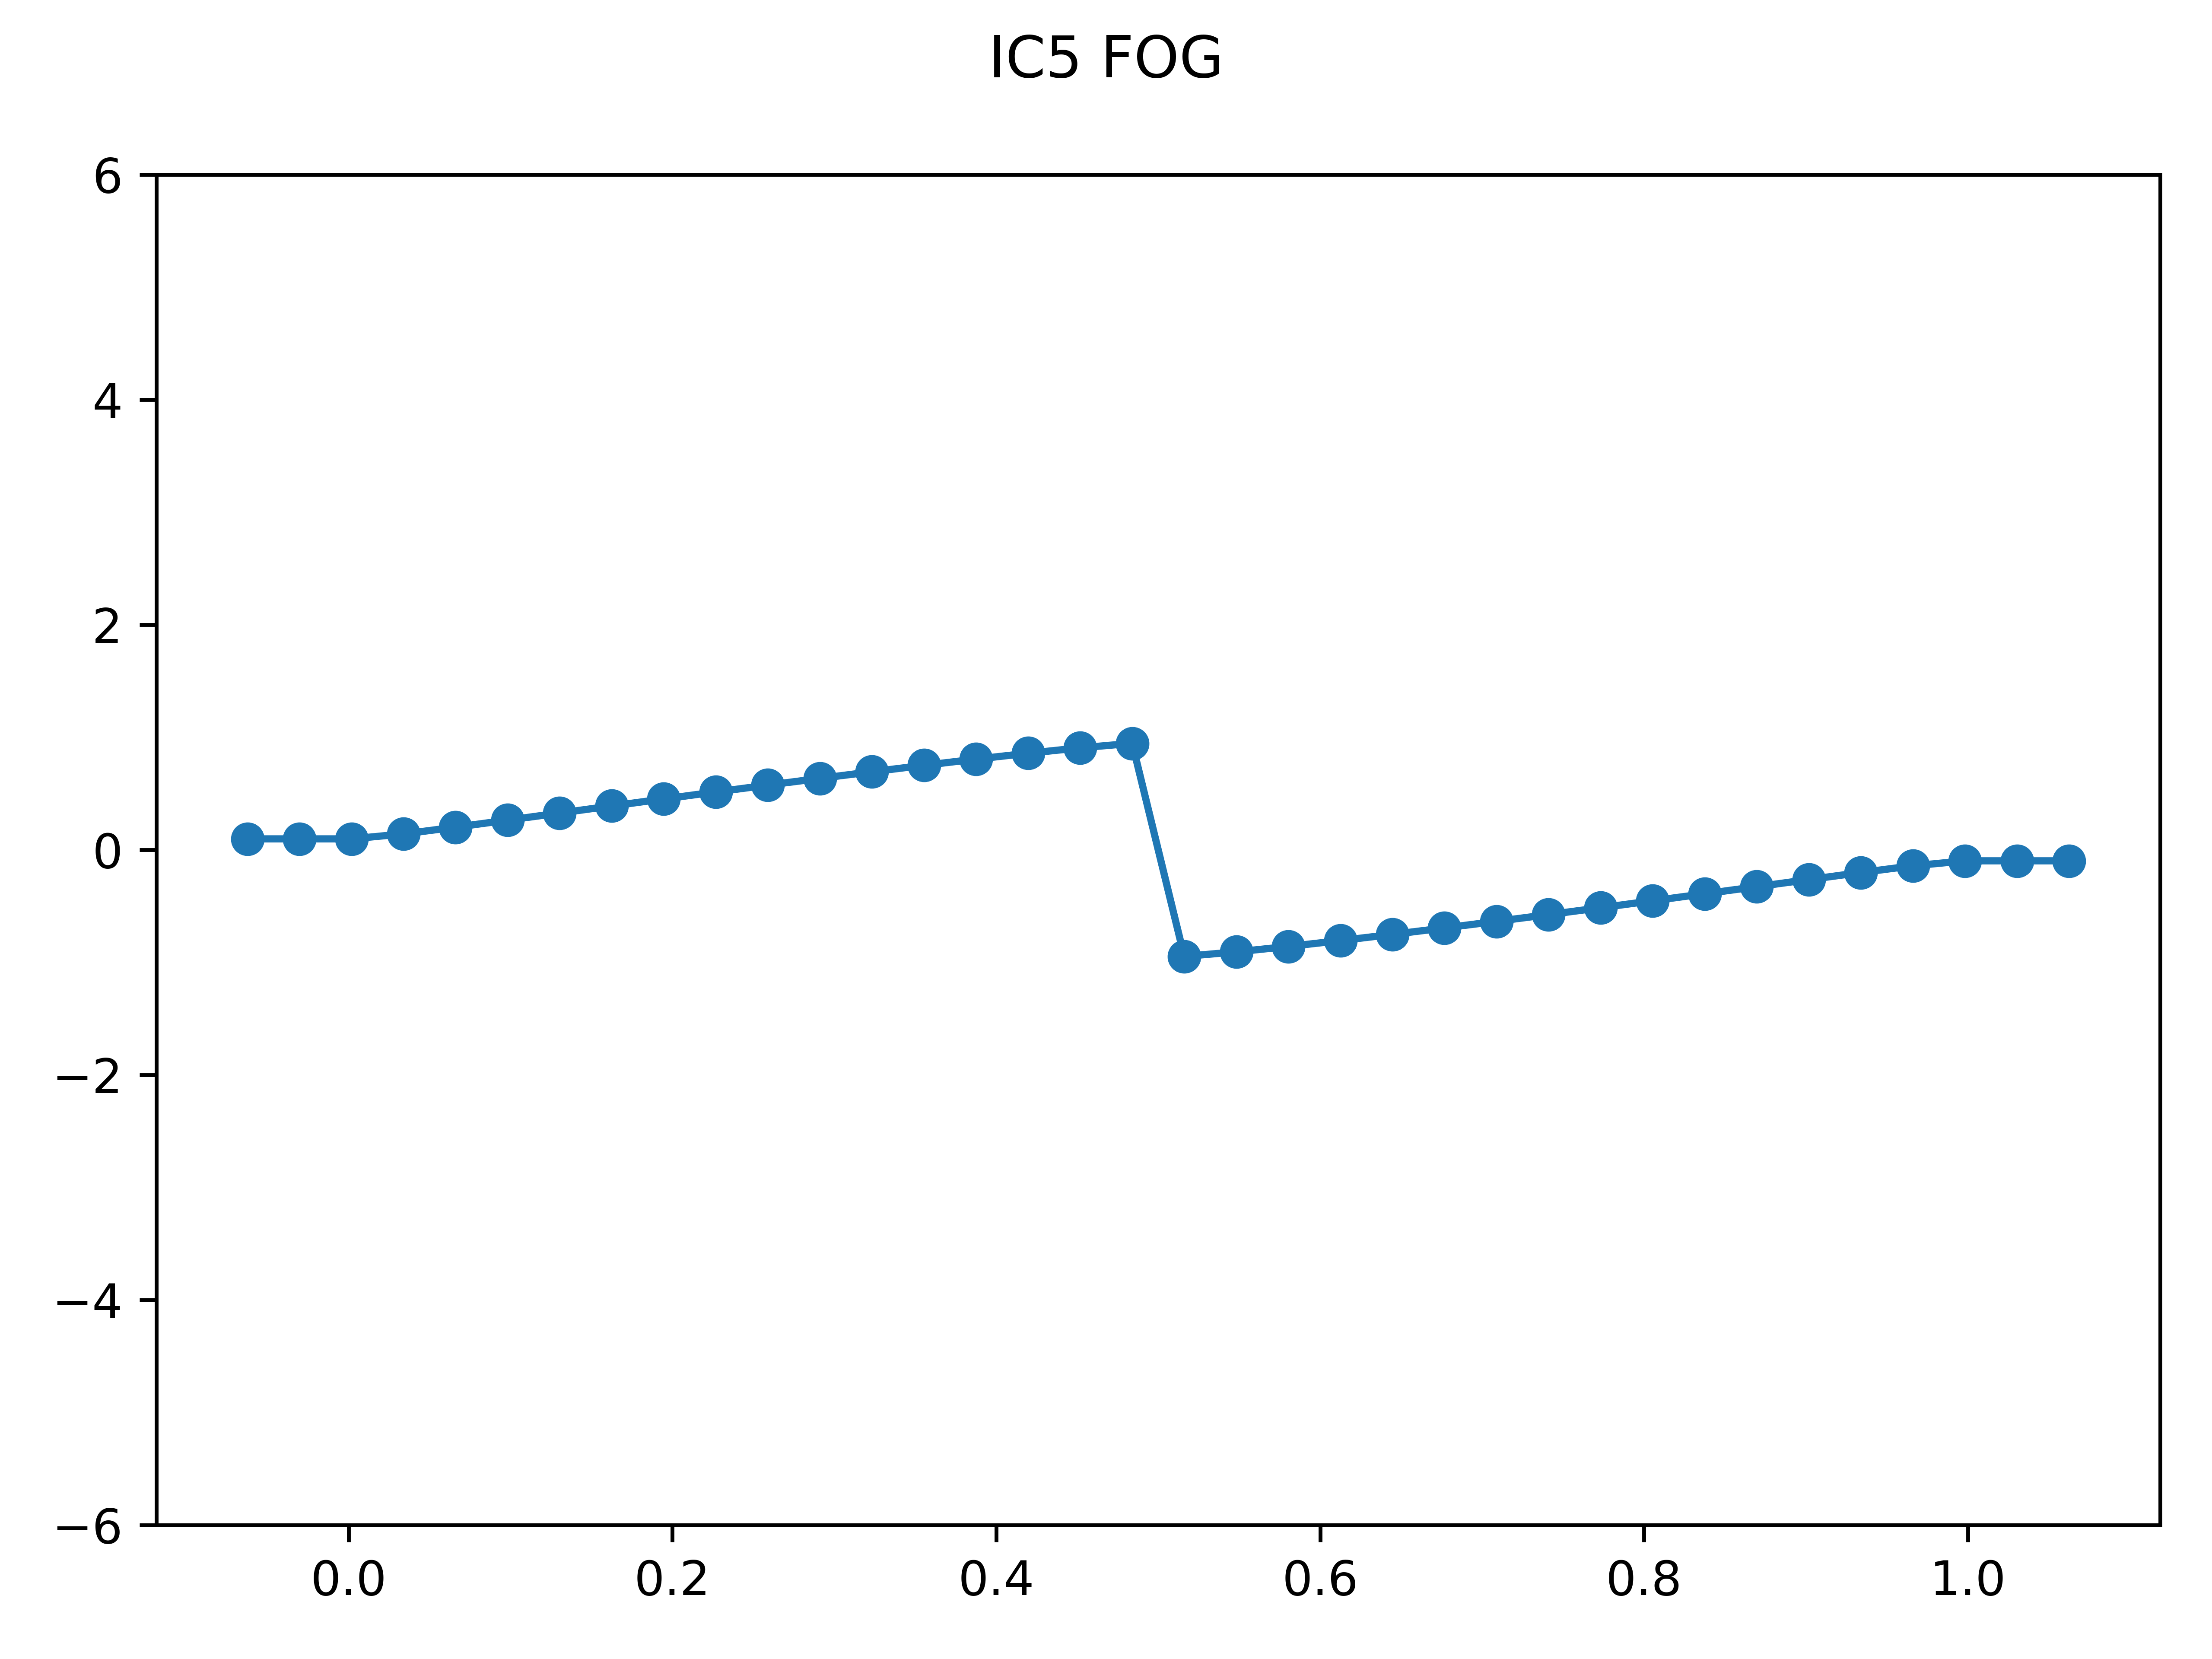
\includegraphics[width=.95\textwidth]{../../code/IC5Methodfu_plot.png}
        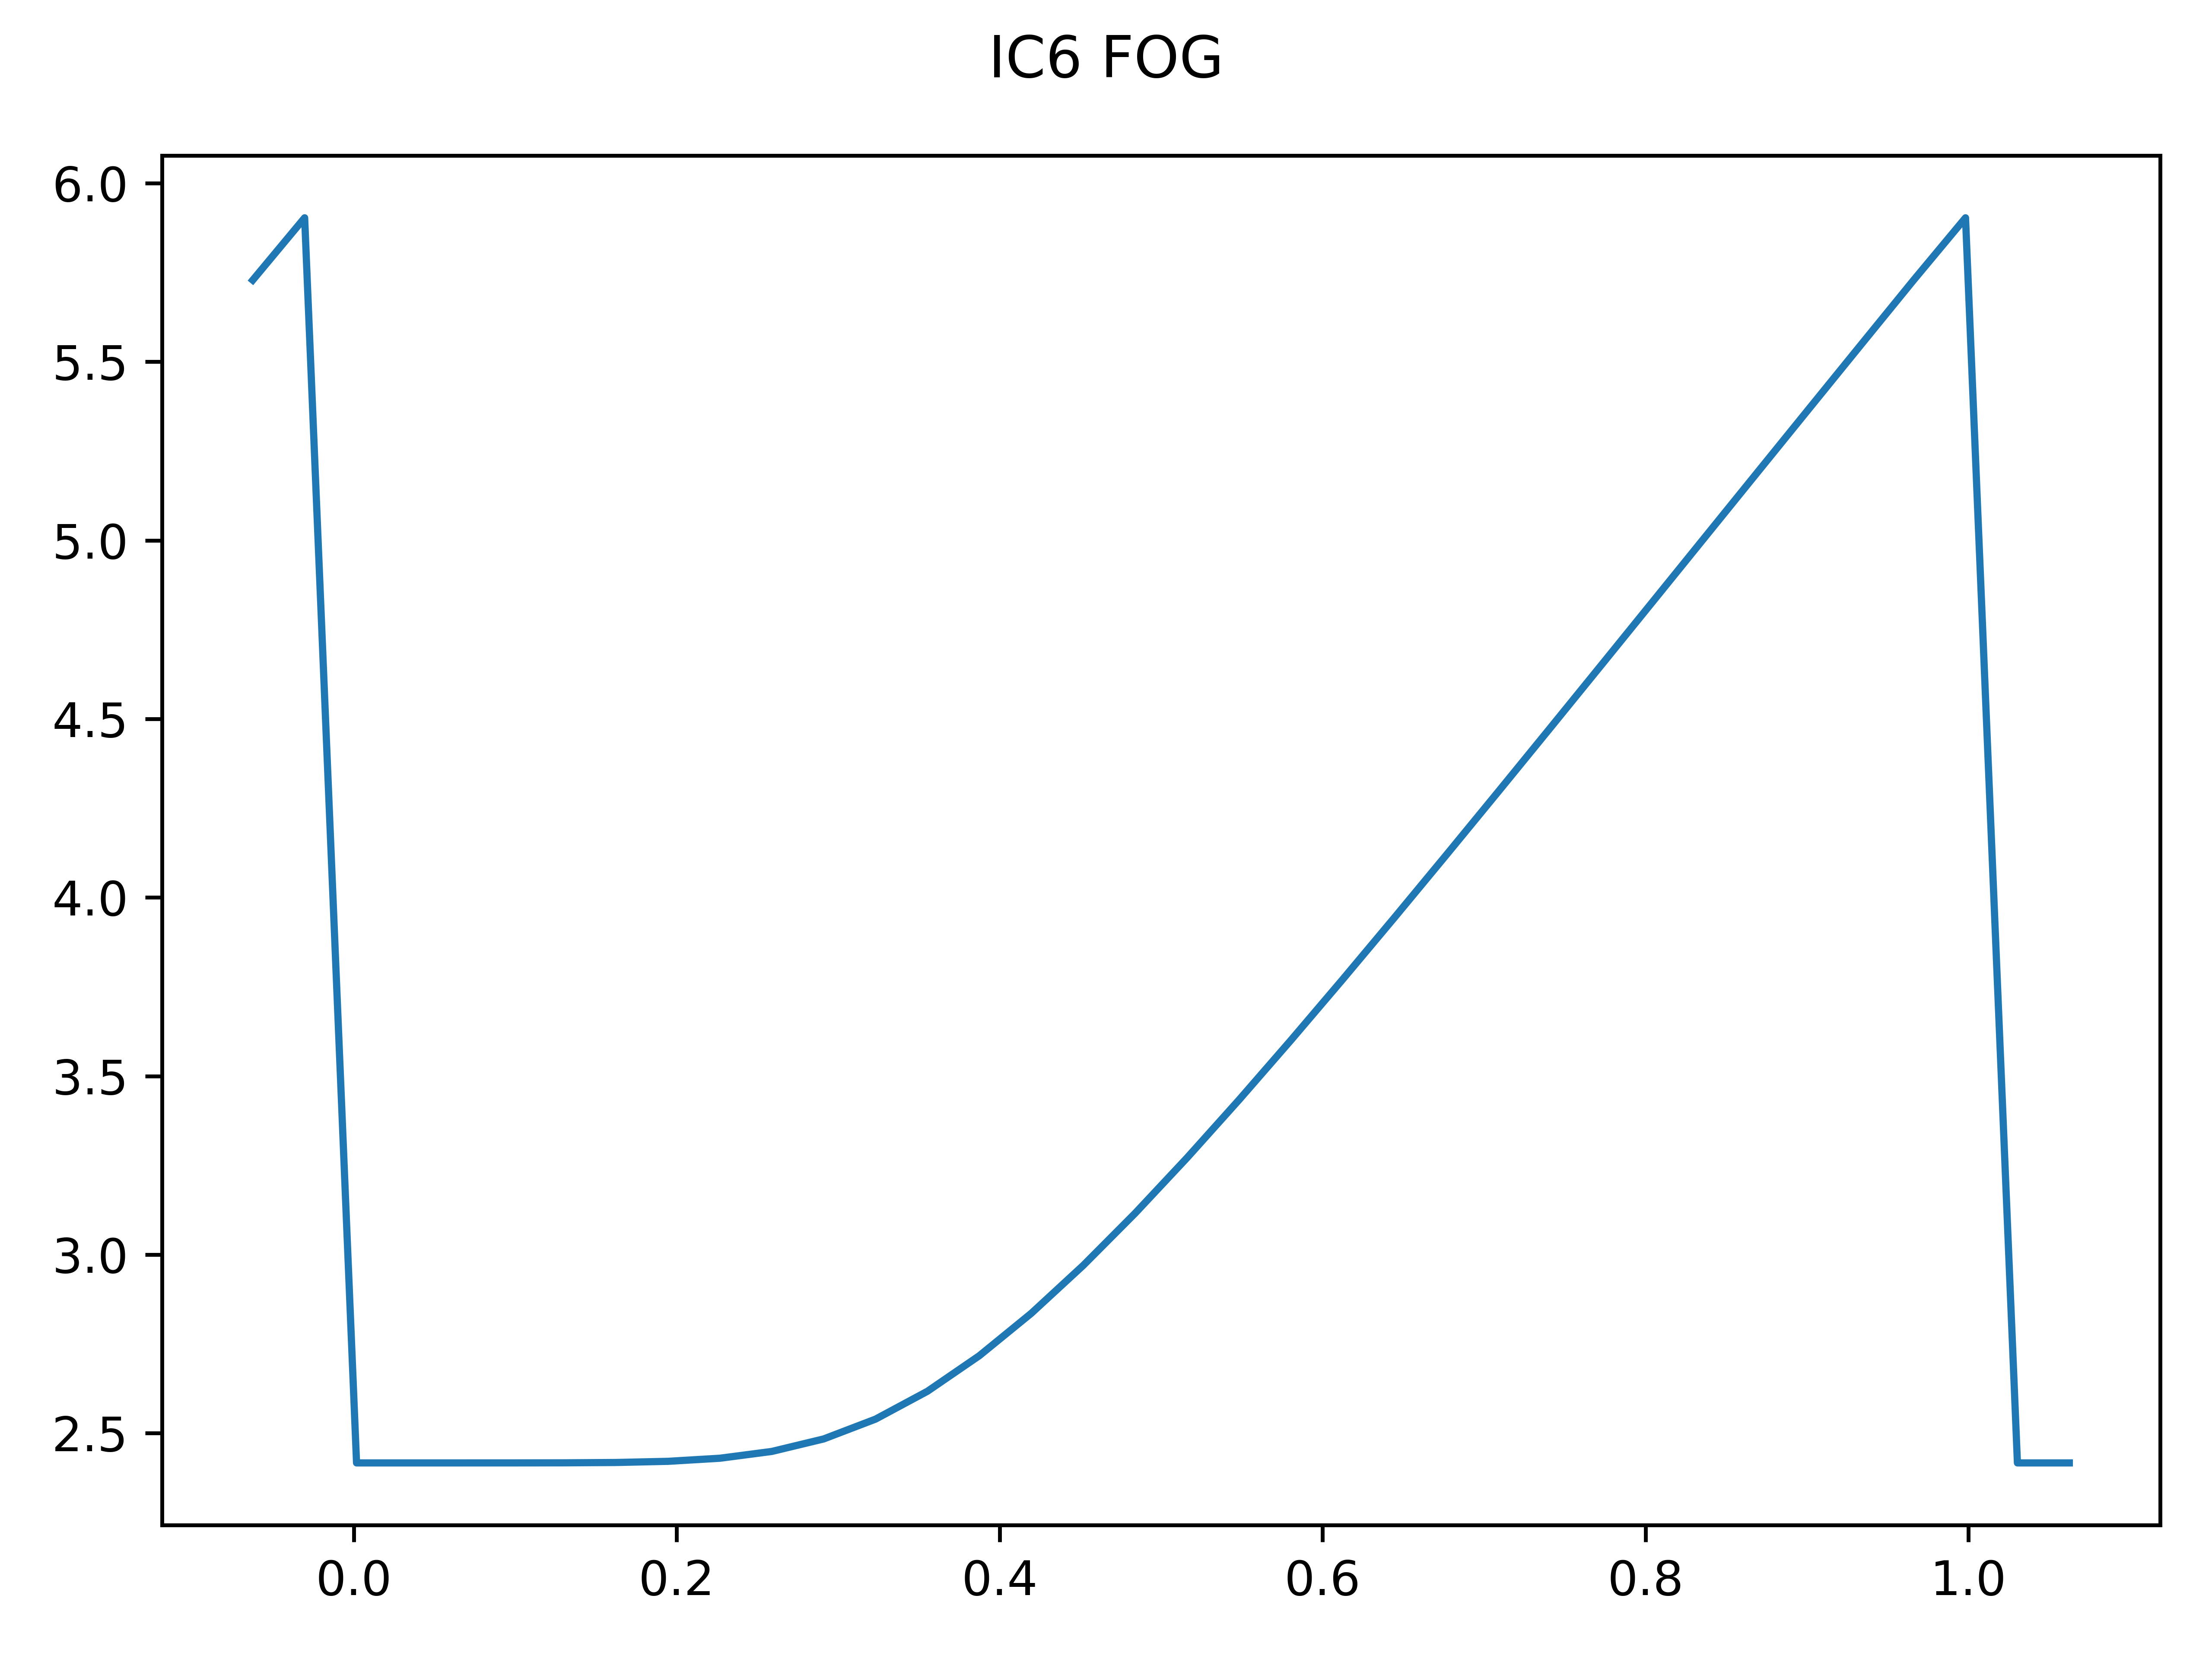
\includegraphics[width=.95\textwidth]{../../code/IC6Methodfu_plot.png}
    \emp
    \bmp{0.25}
        \centering
        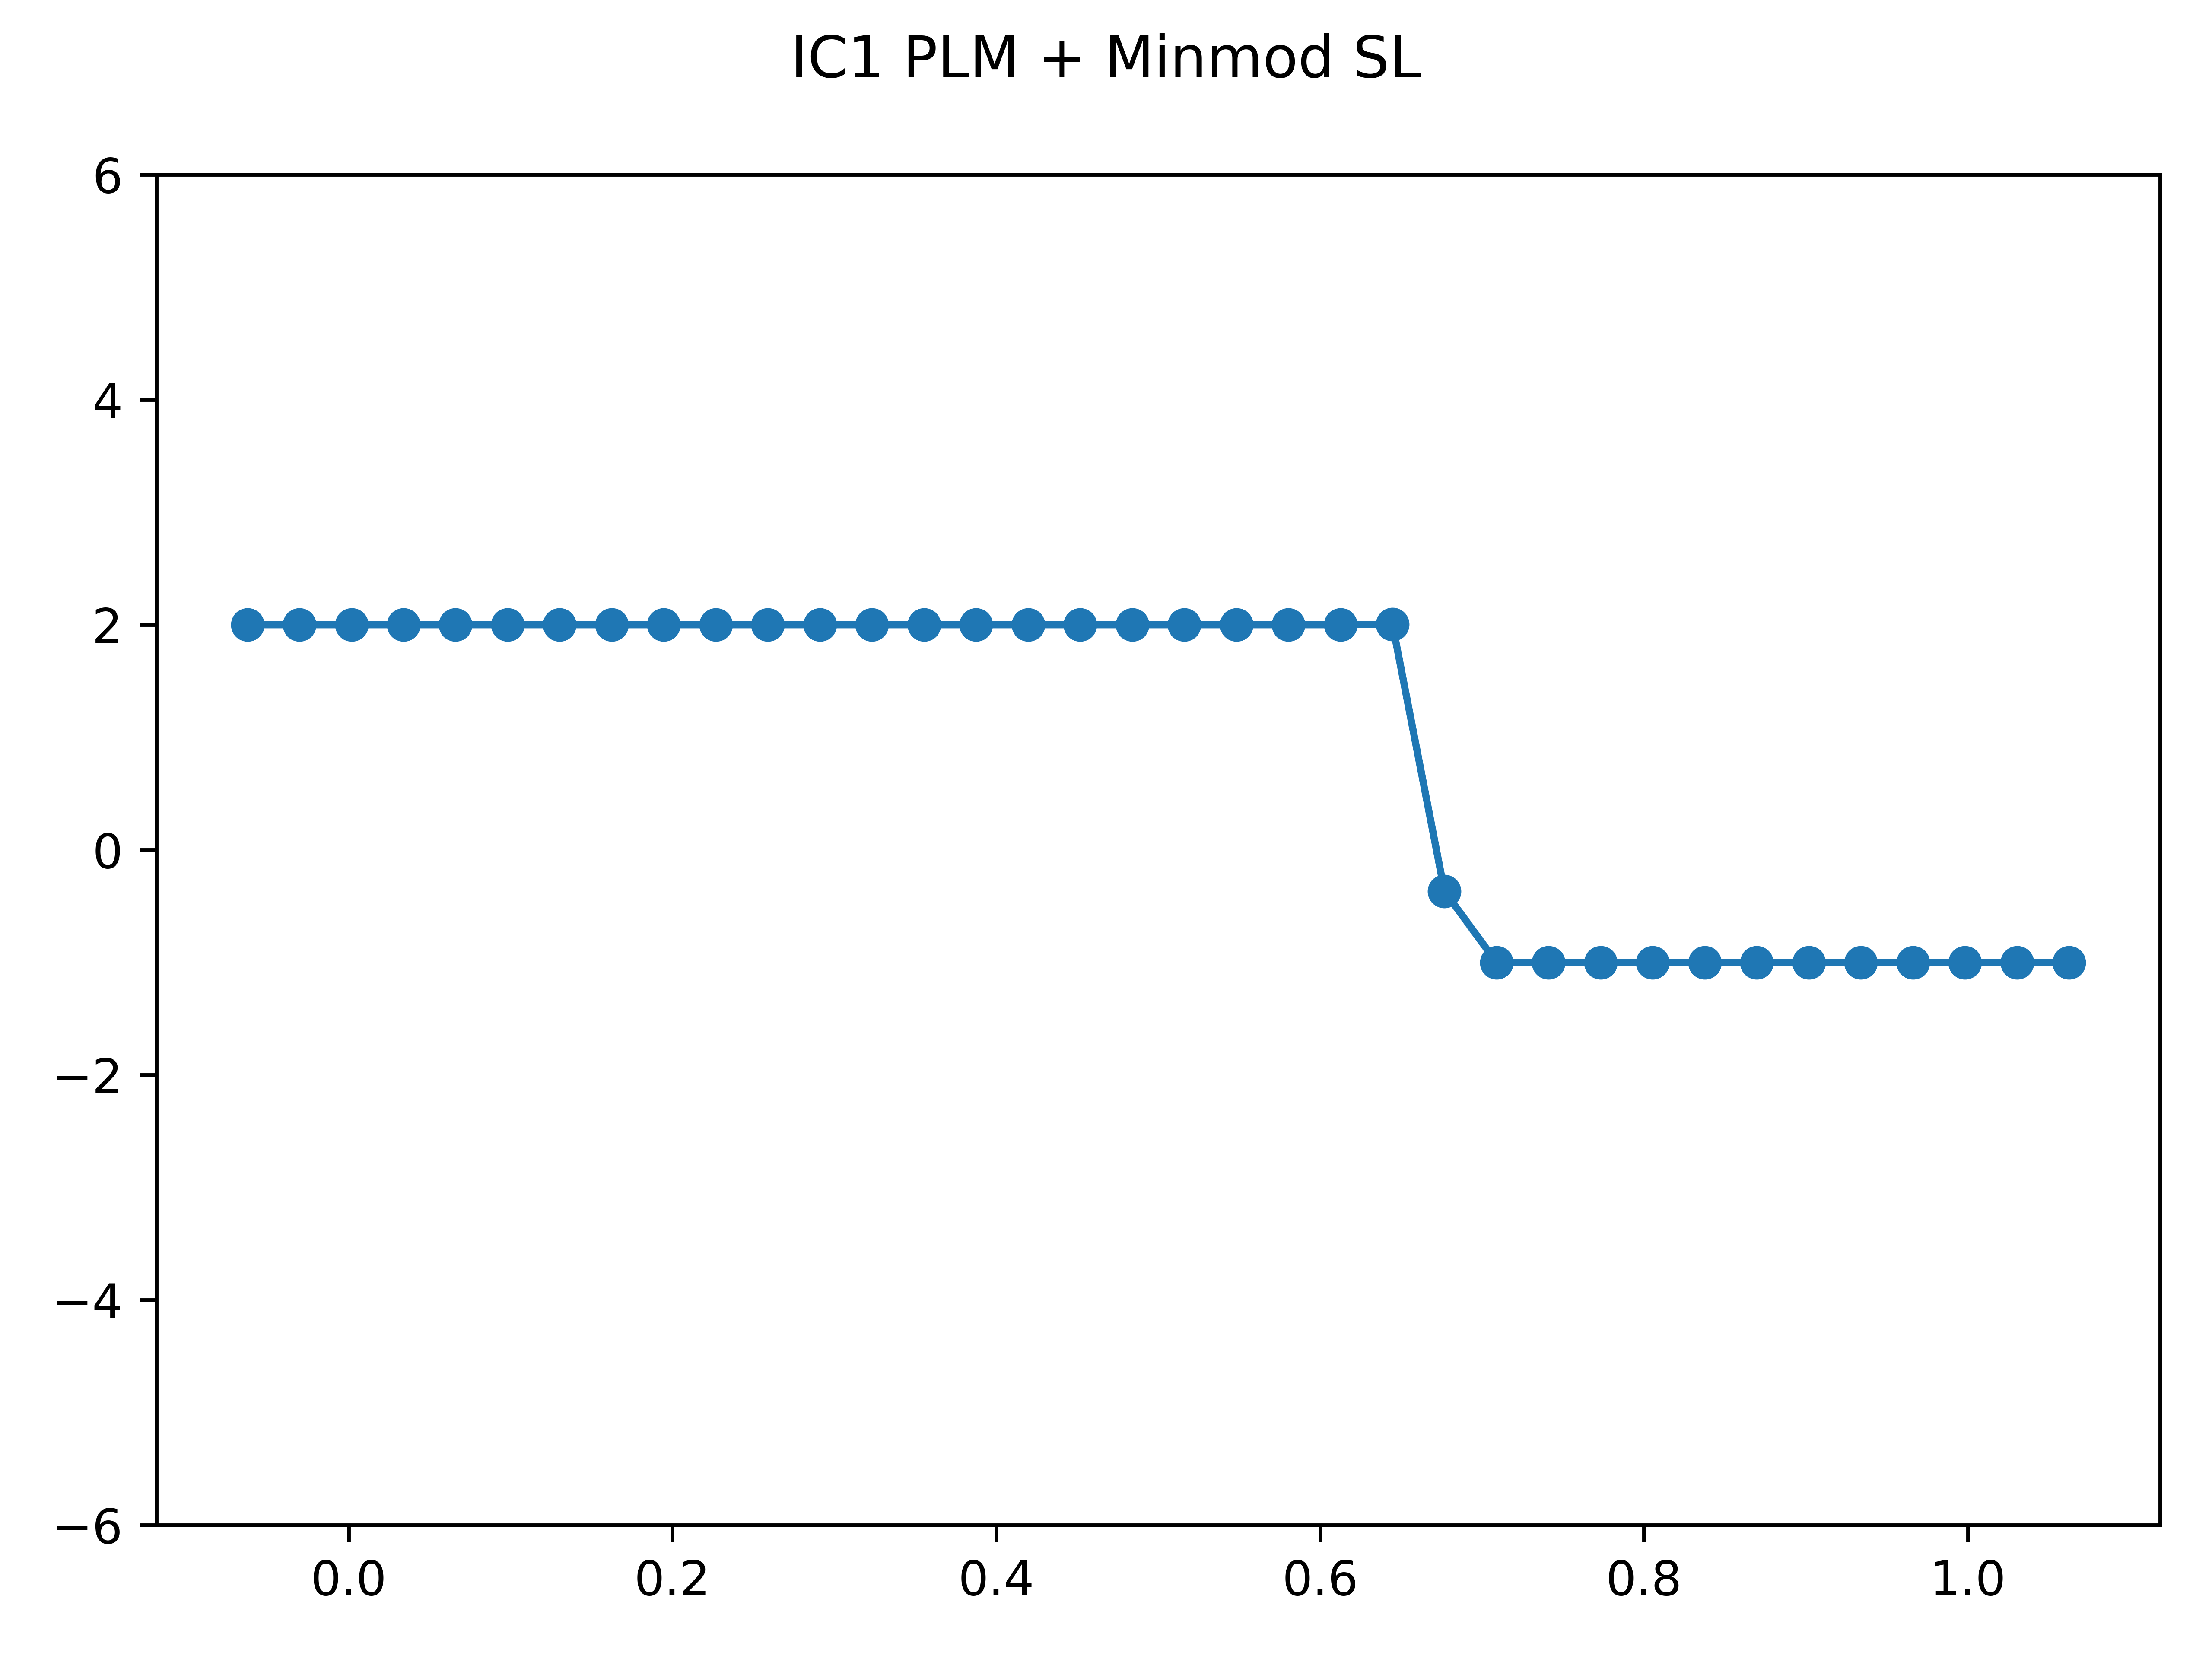
\includegraphics[width=.95\textwidth]{../../code/IC1Methodpm_plot.png}
        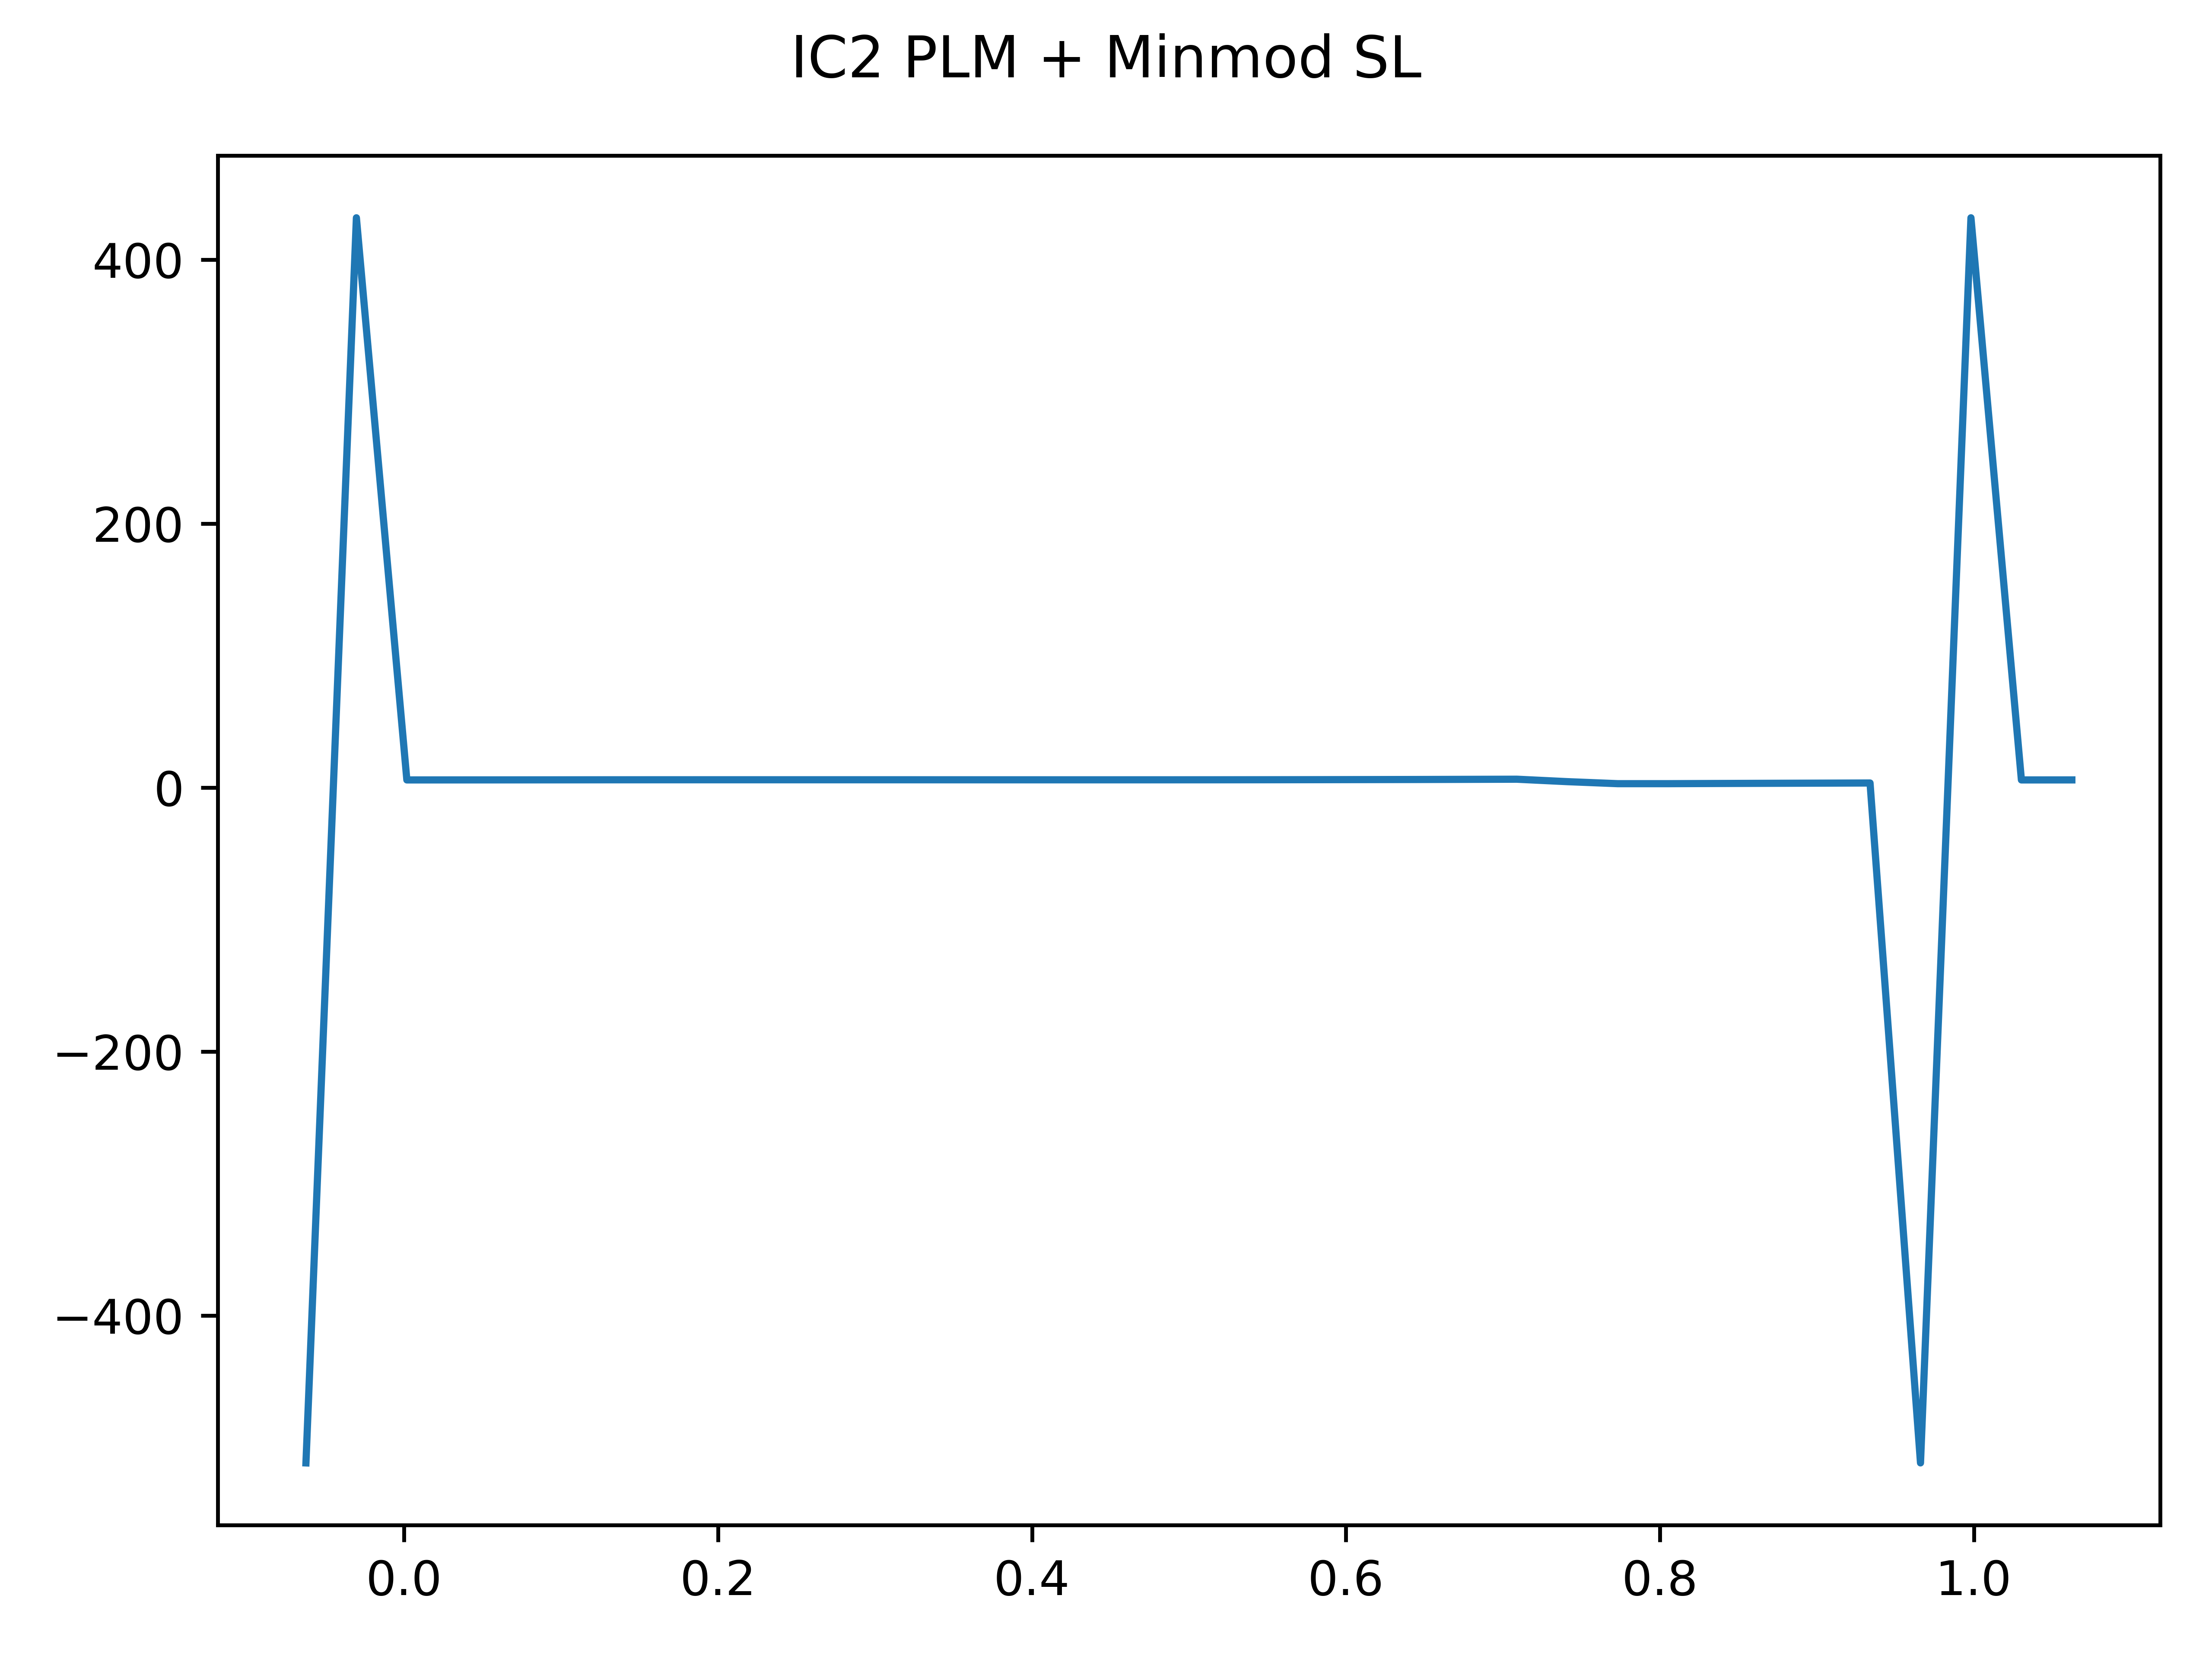
\includegraphics[width=.95\textwidth]{../../code/IC2Methodpm_plot.png}
        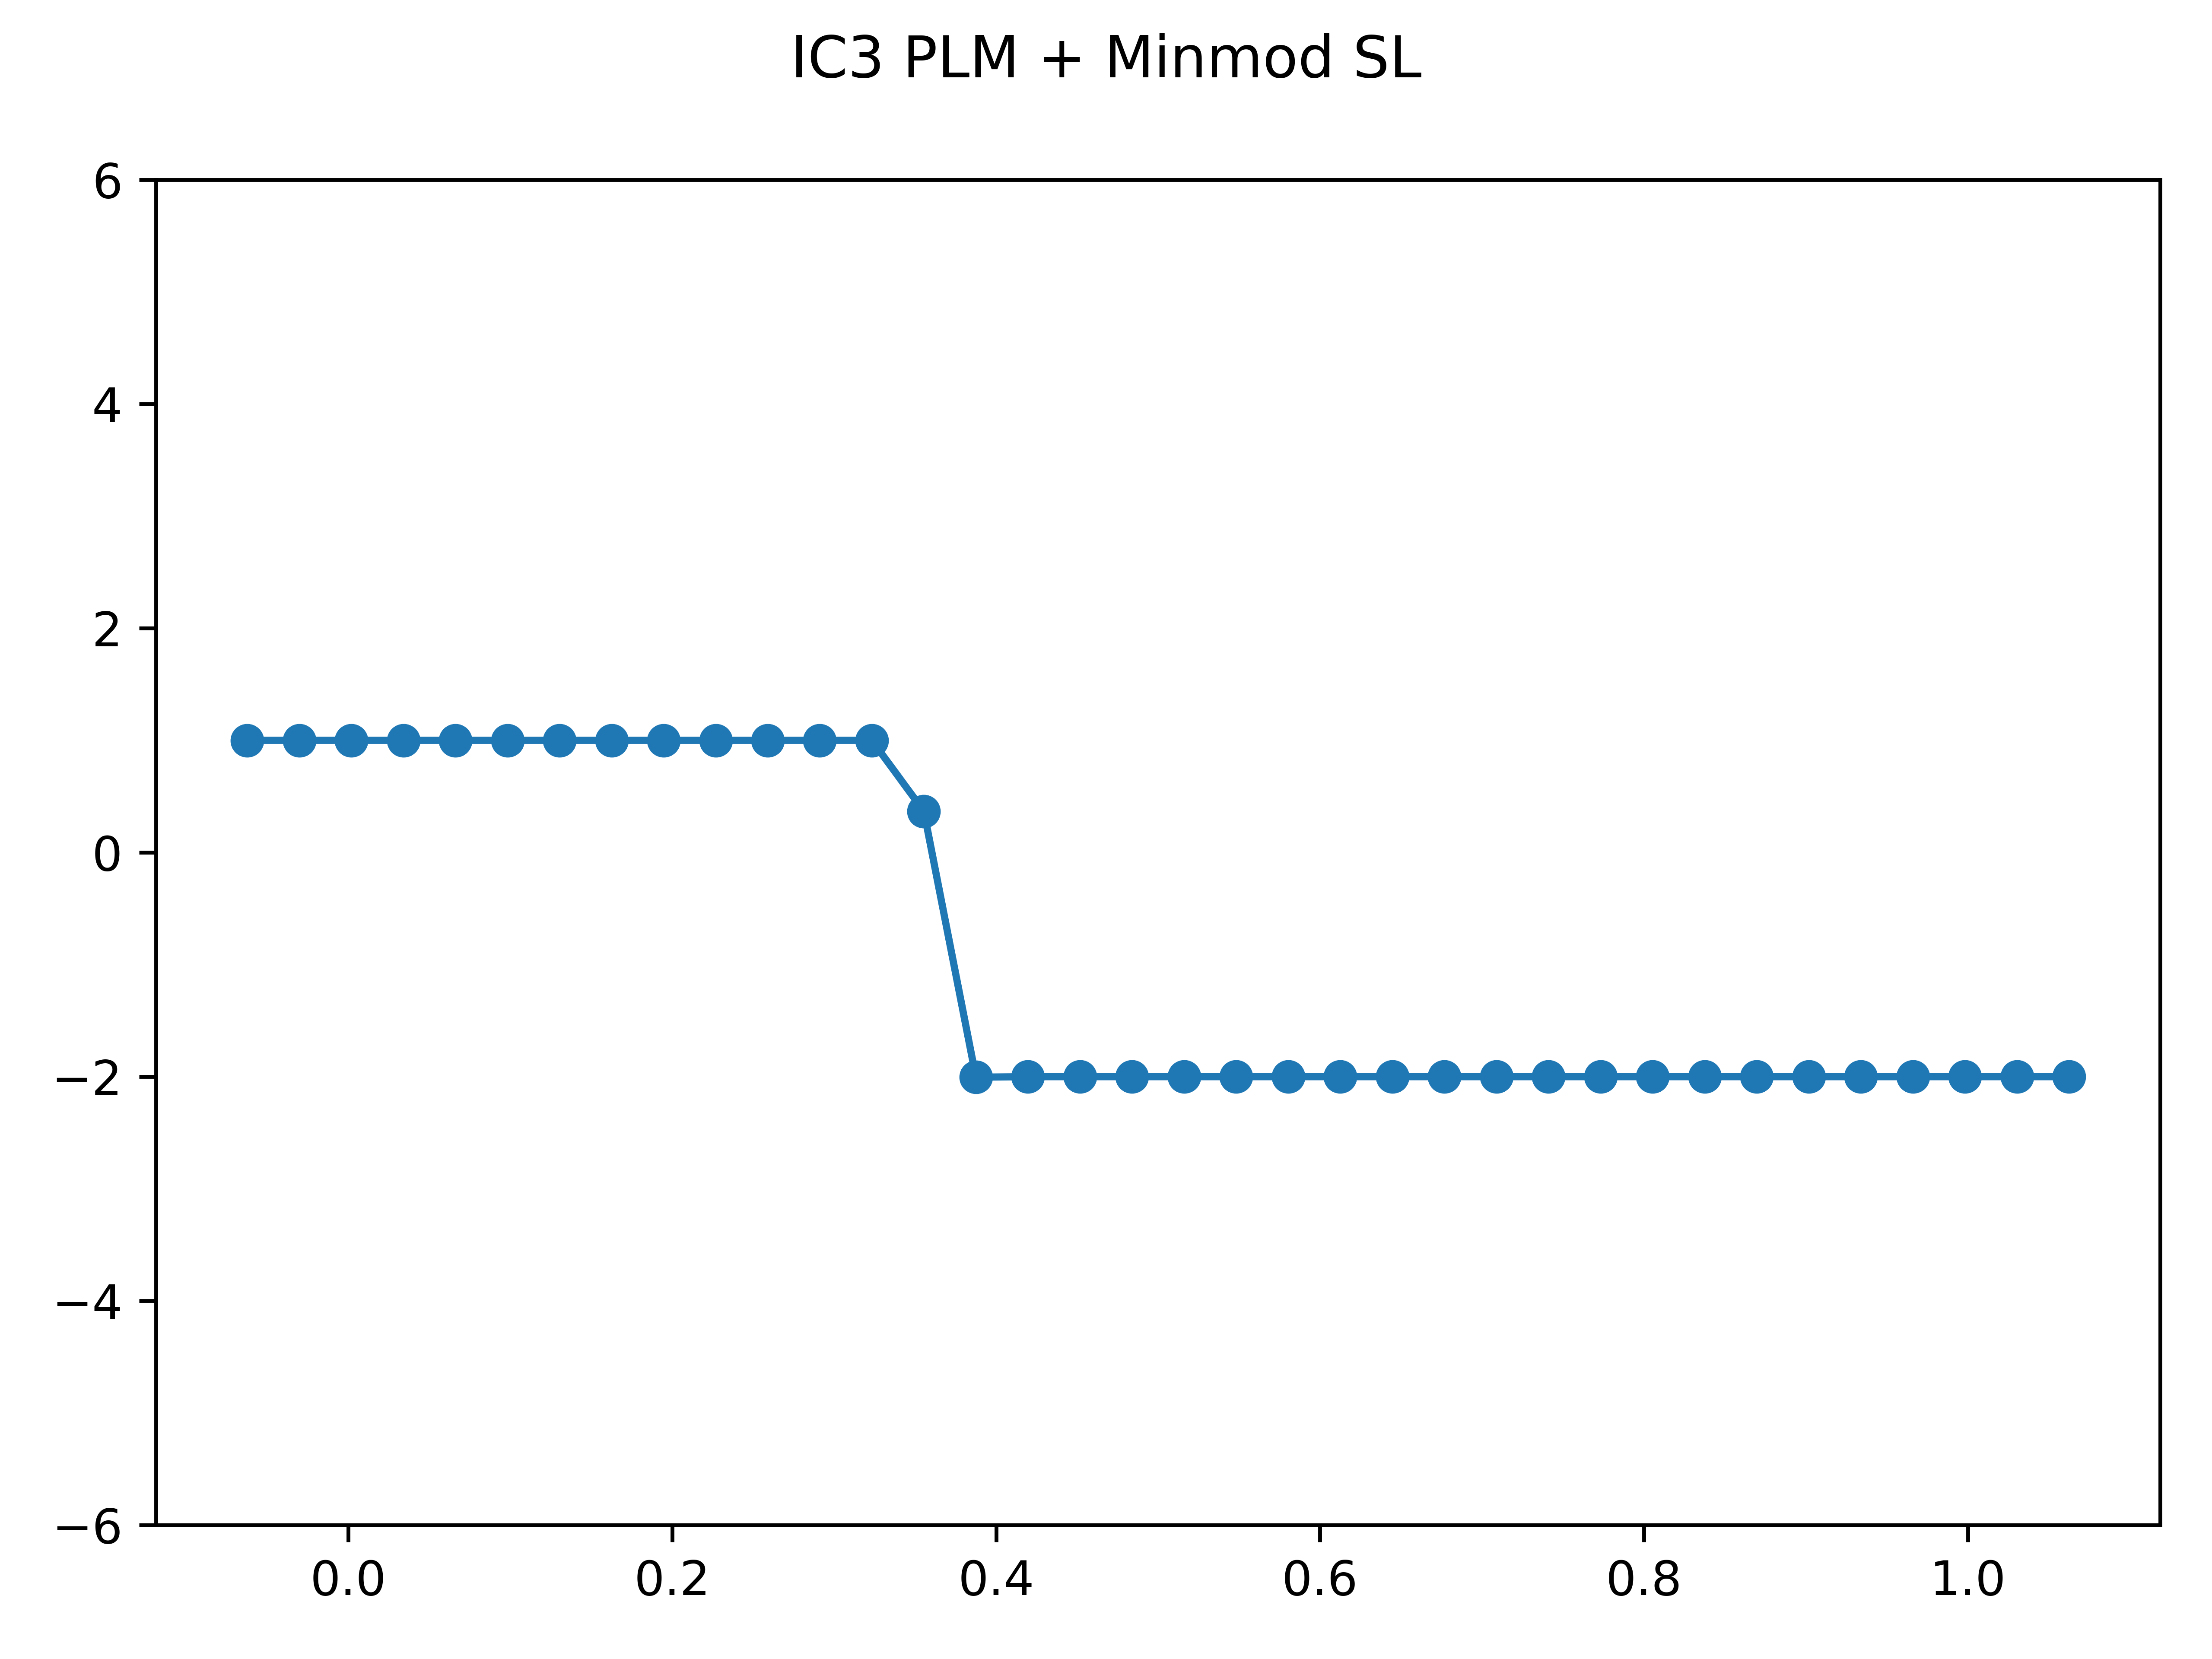
\includegraphics[width=.95\textwidth]{../../code/IC3Methodpm_plot.png}
        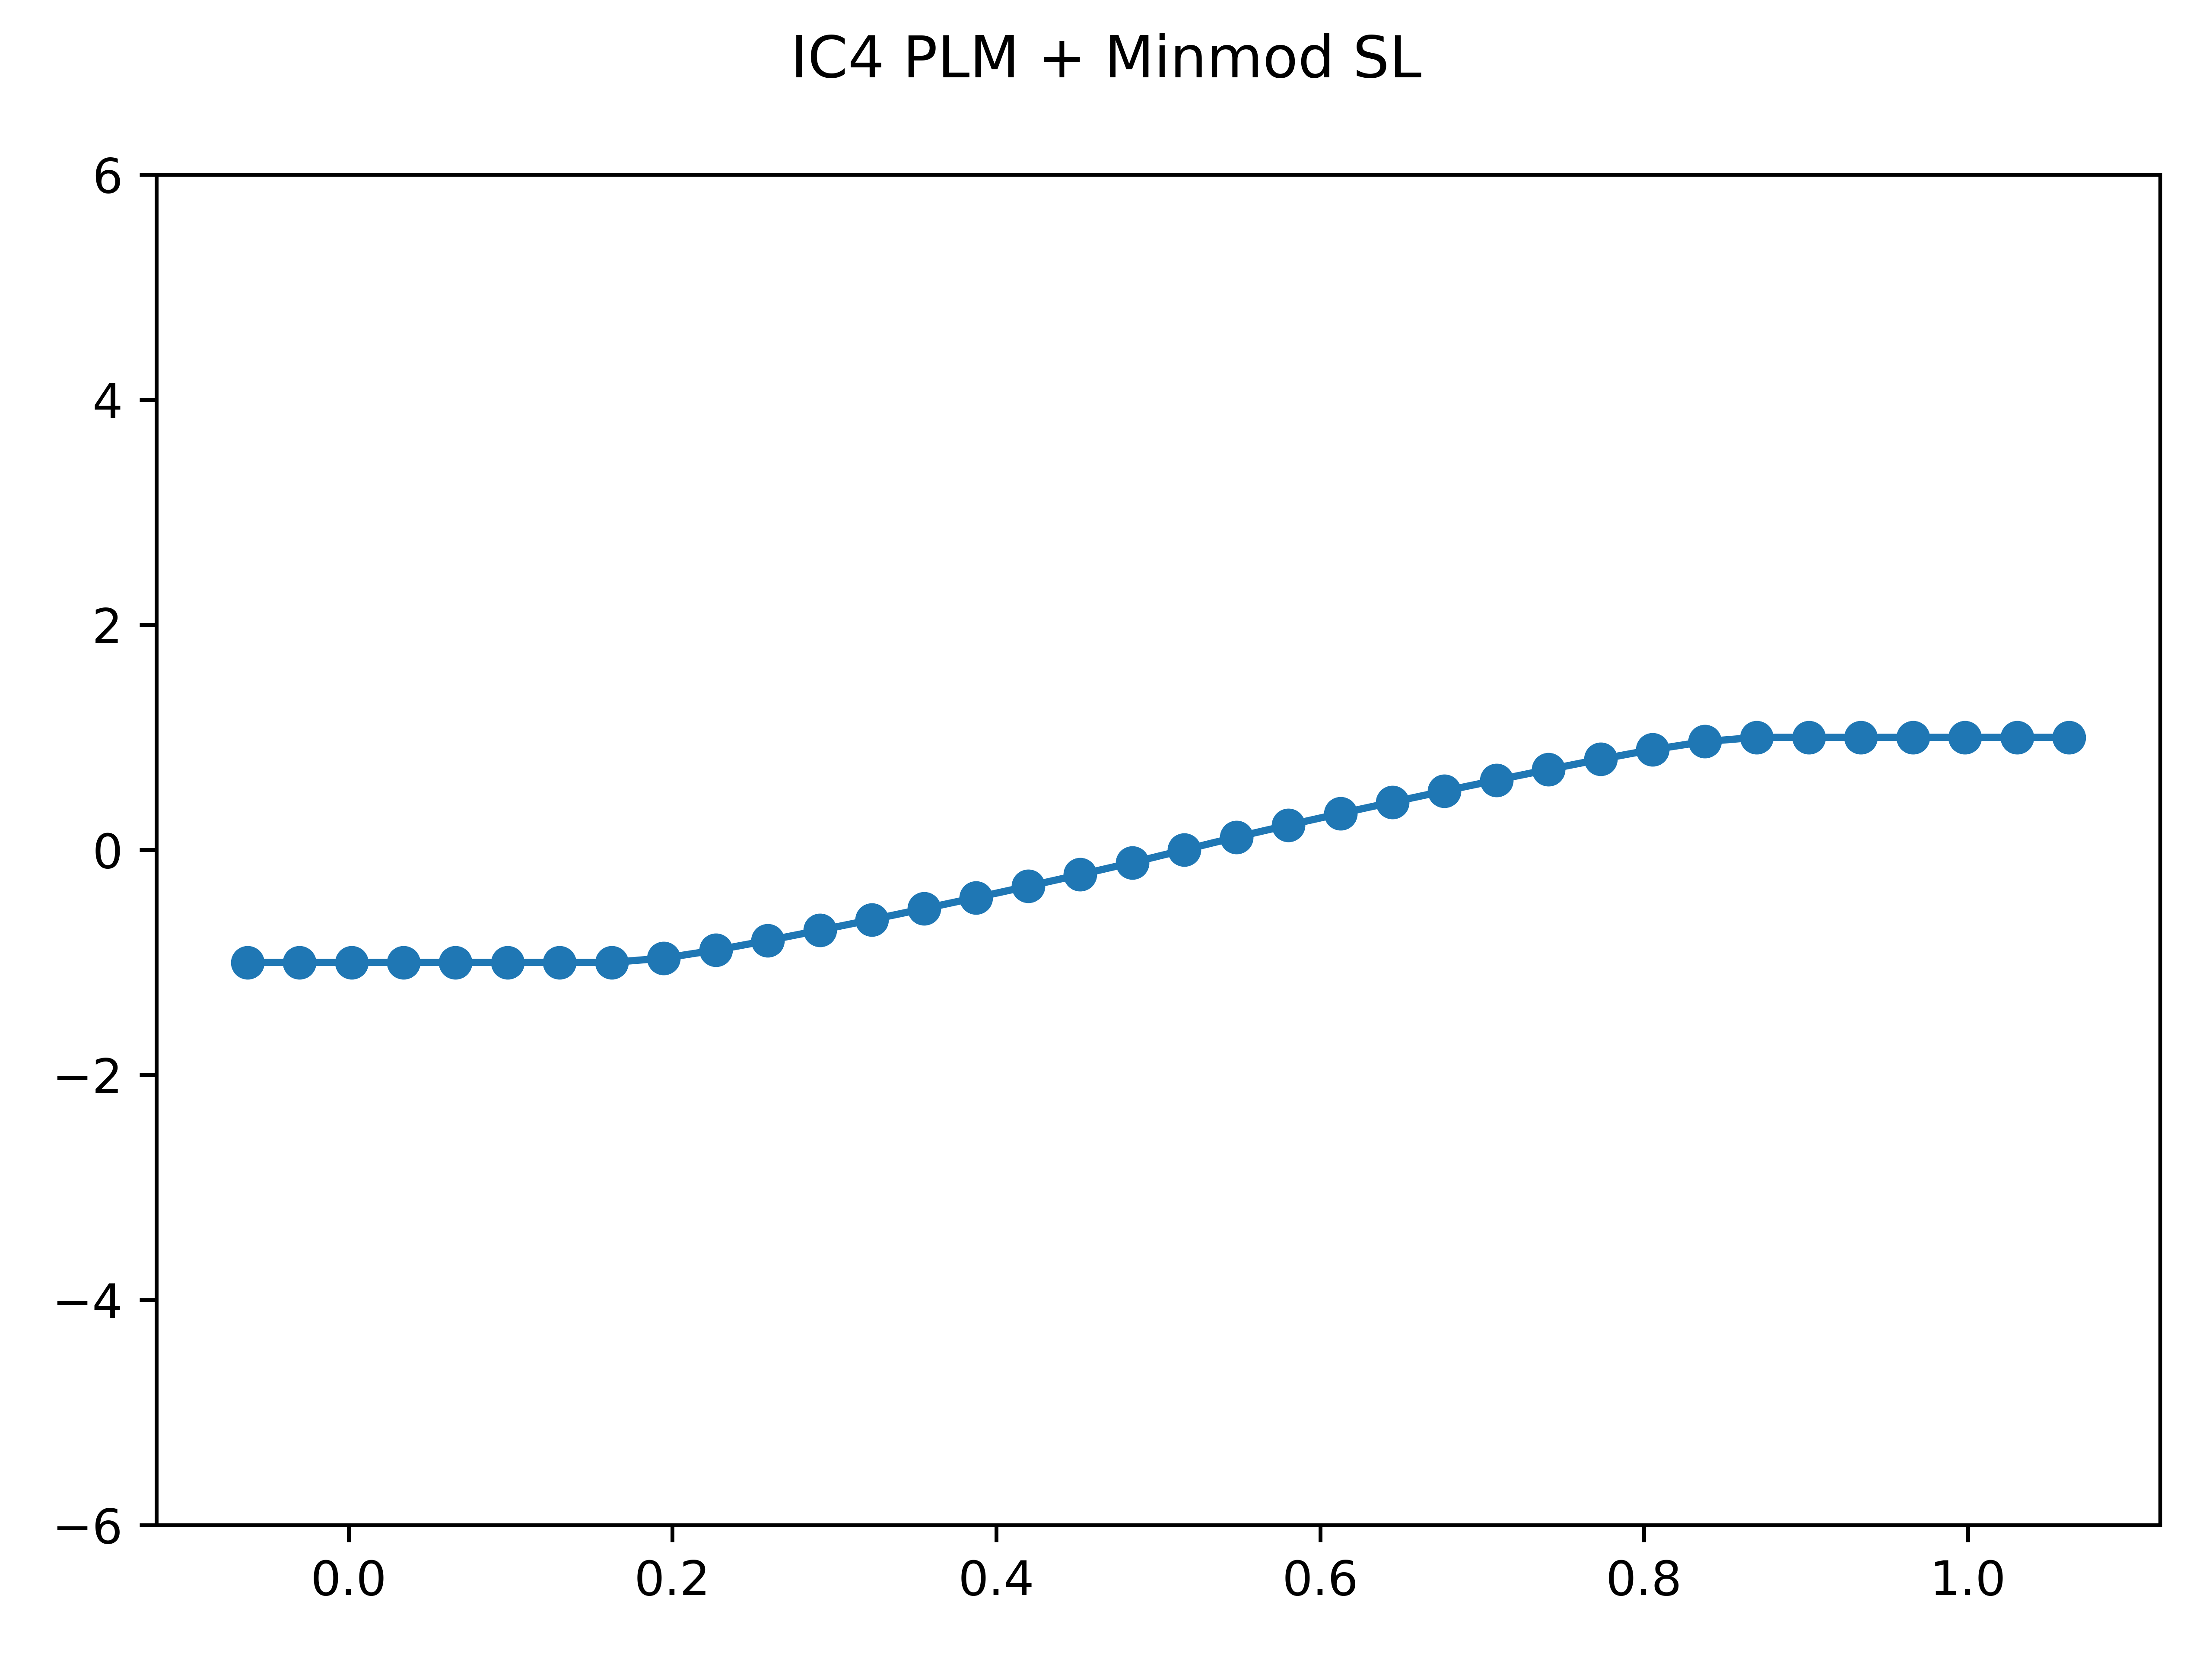
\includegraphics[width=.95\textwidth]{../../code/IC4Methodpm_plot.png}
        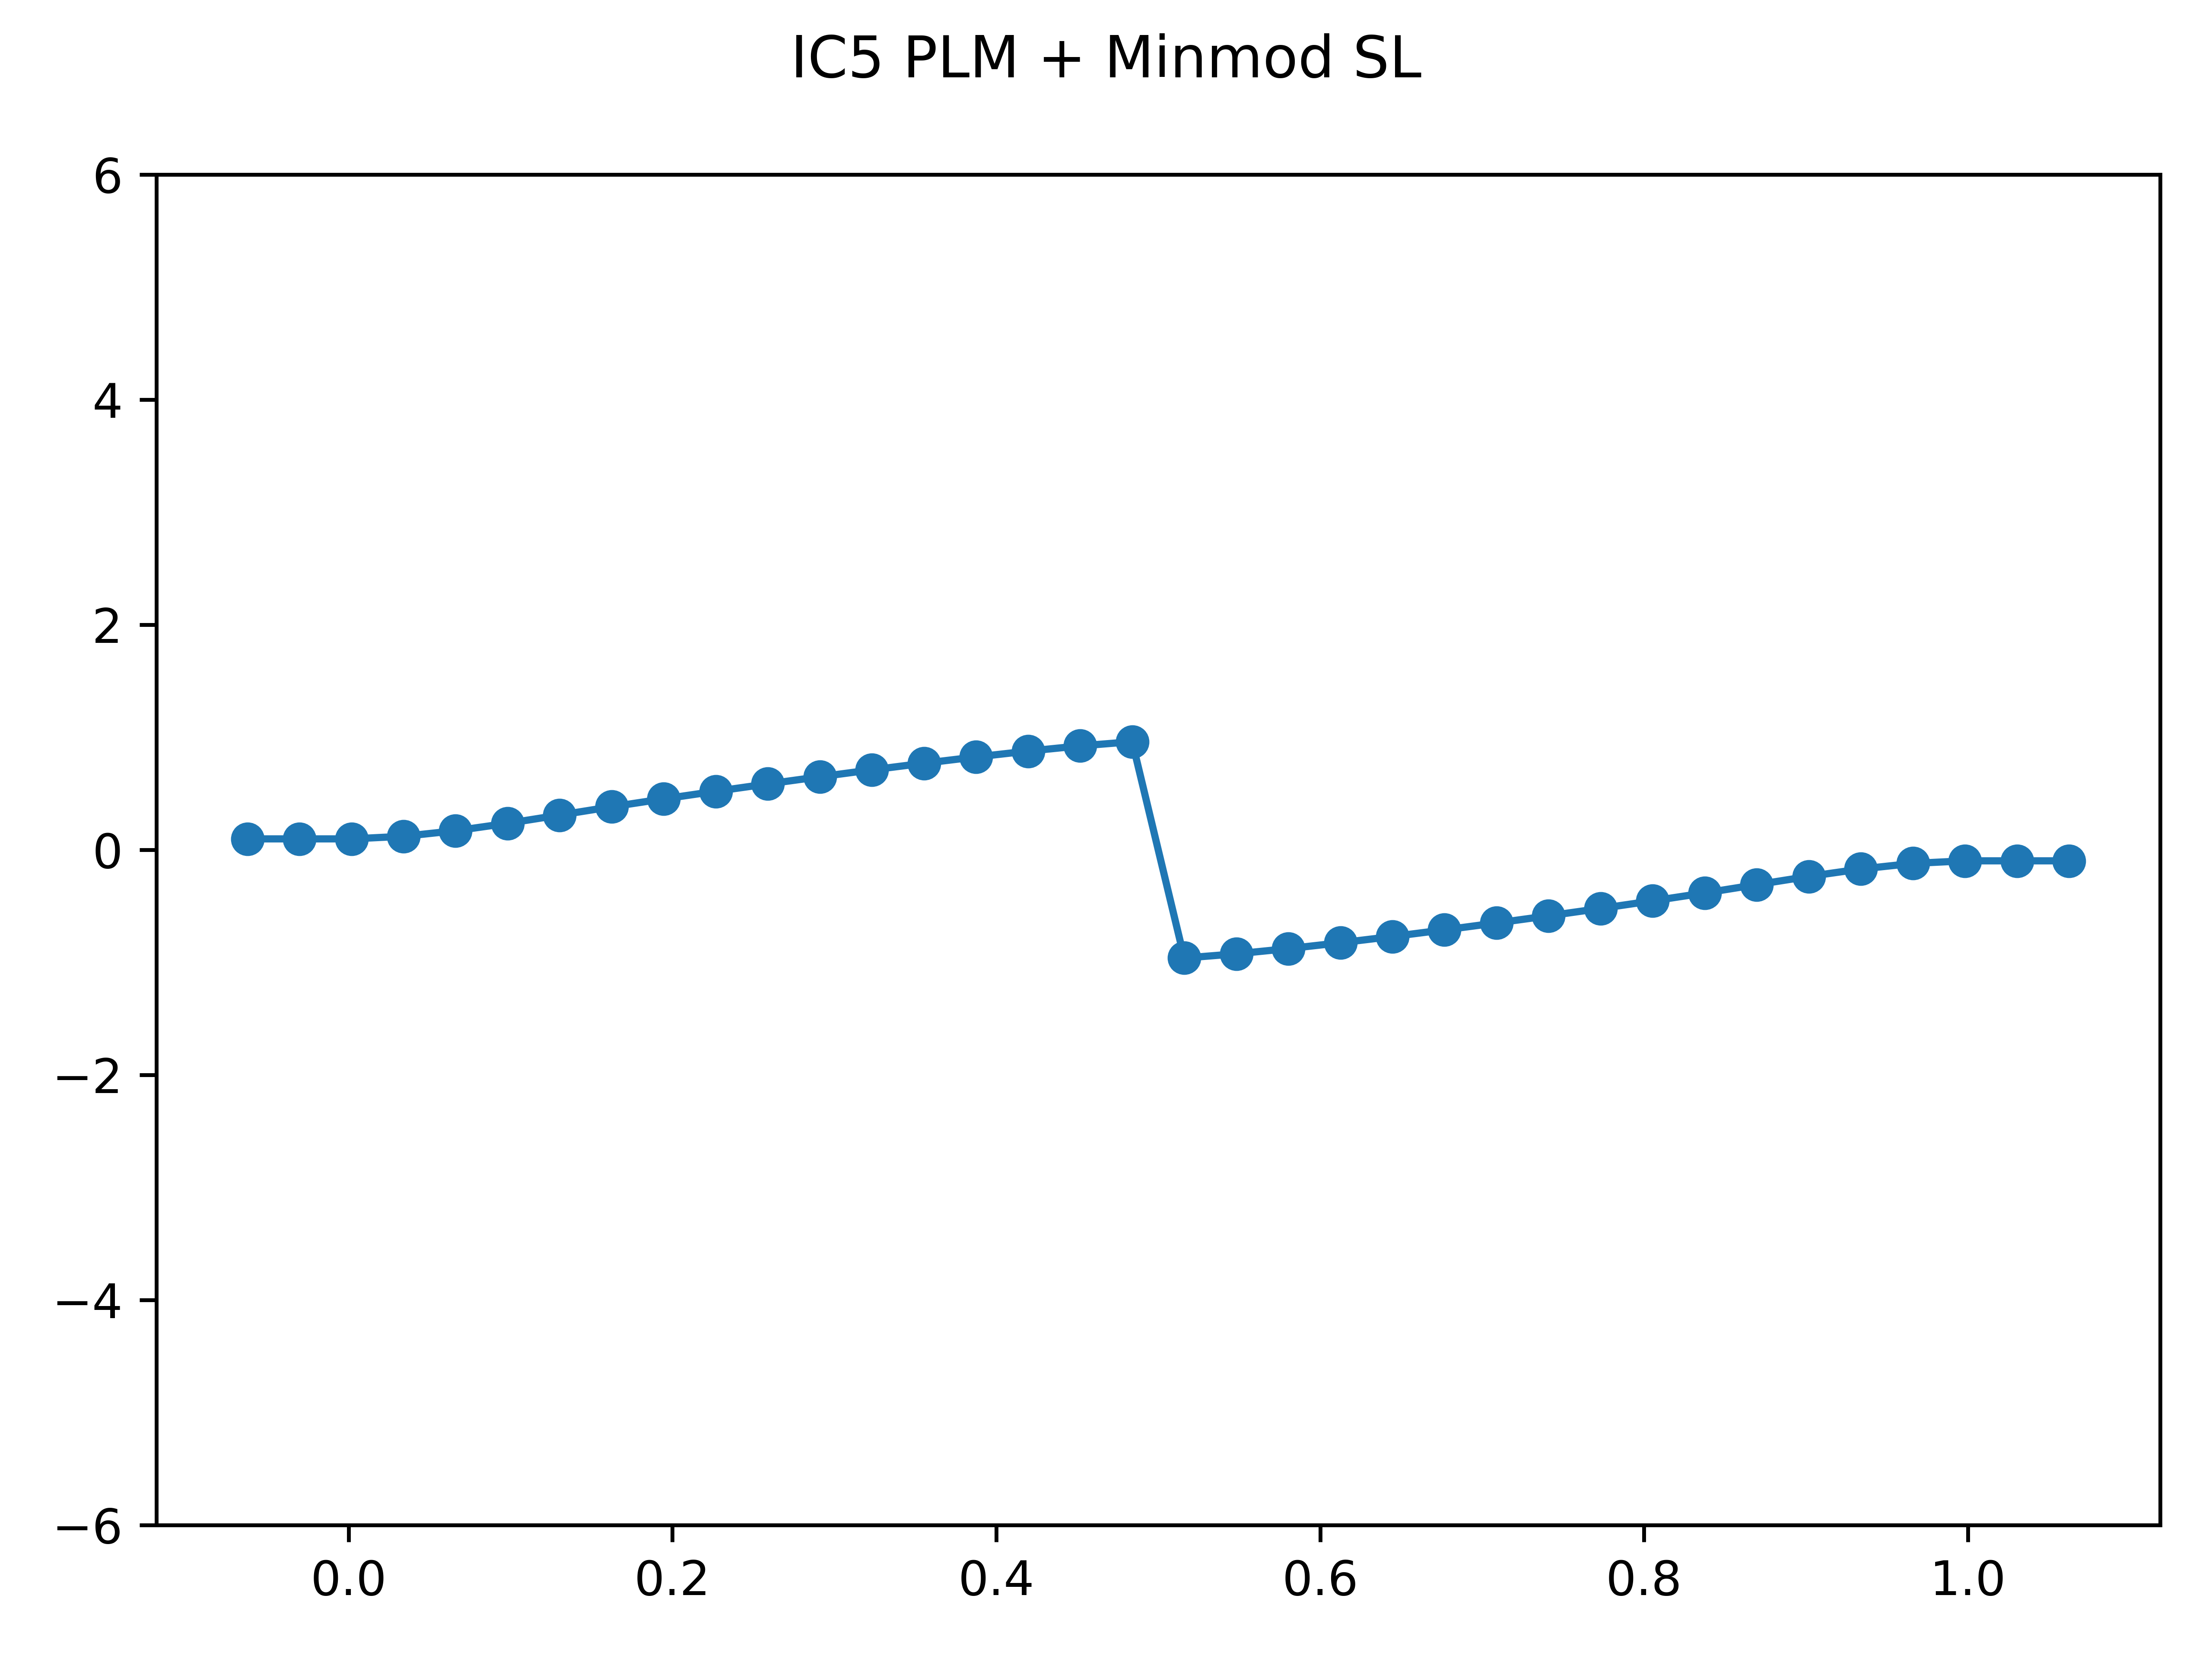
\includegraphics[width=.95\textwidth]{../../code/IC5Methodpm_plot.png}
        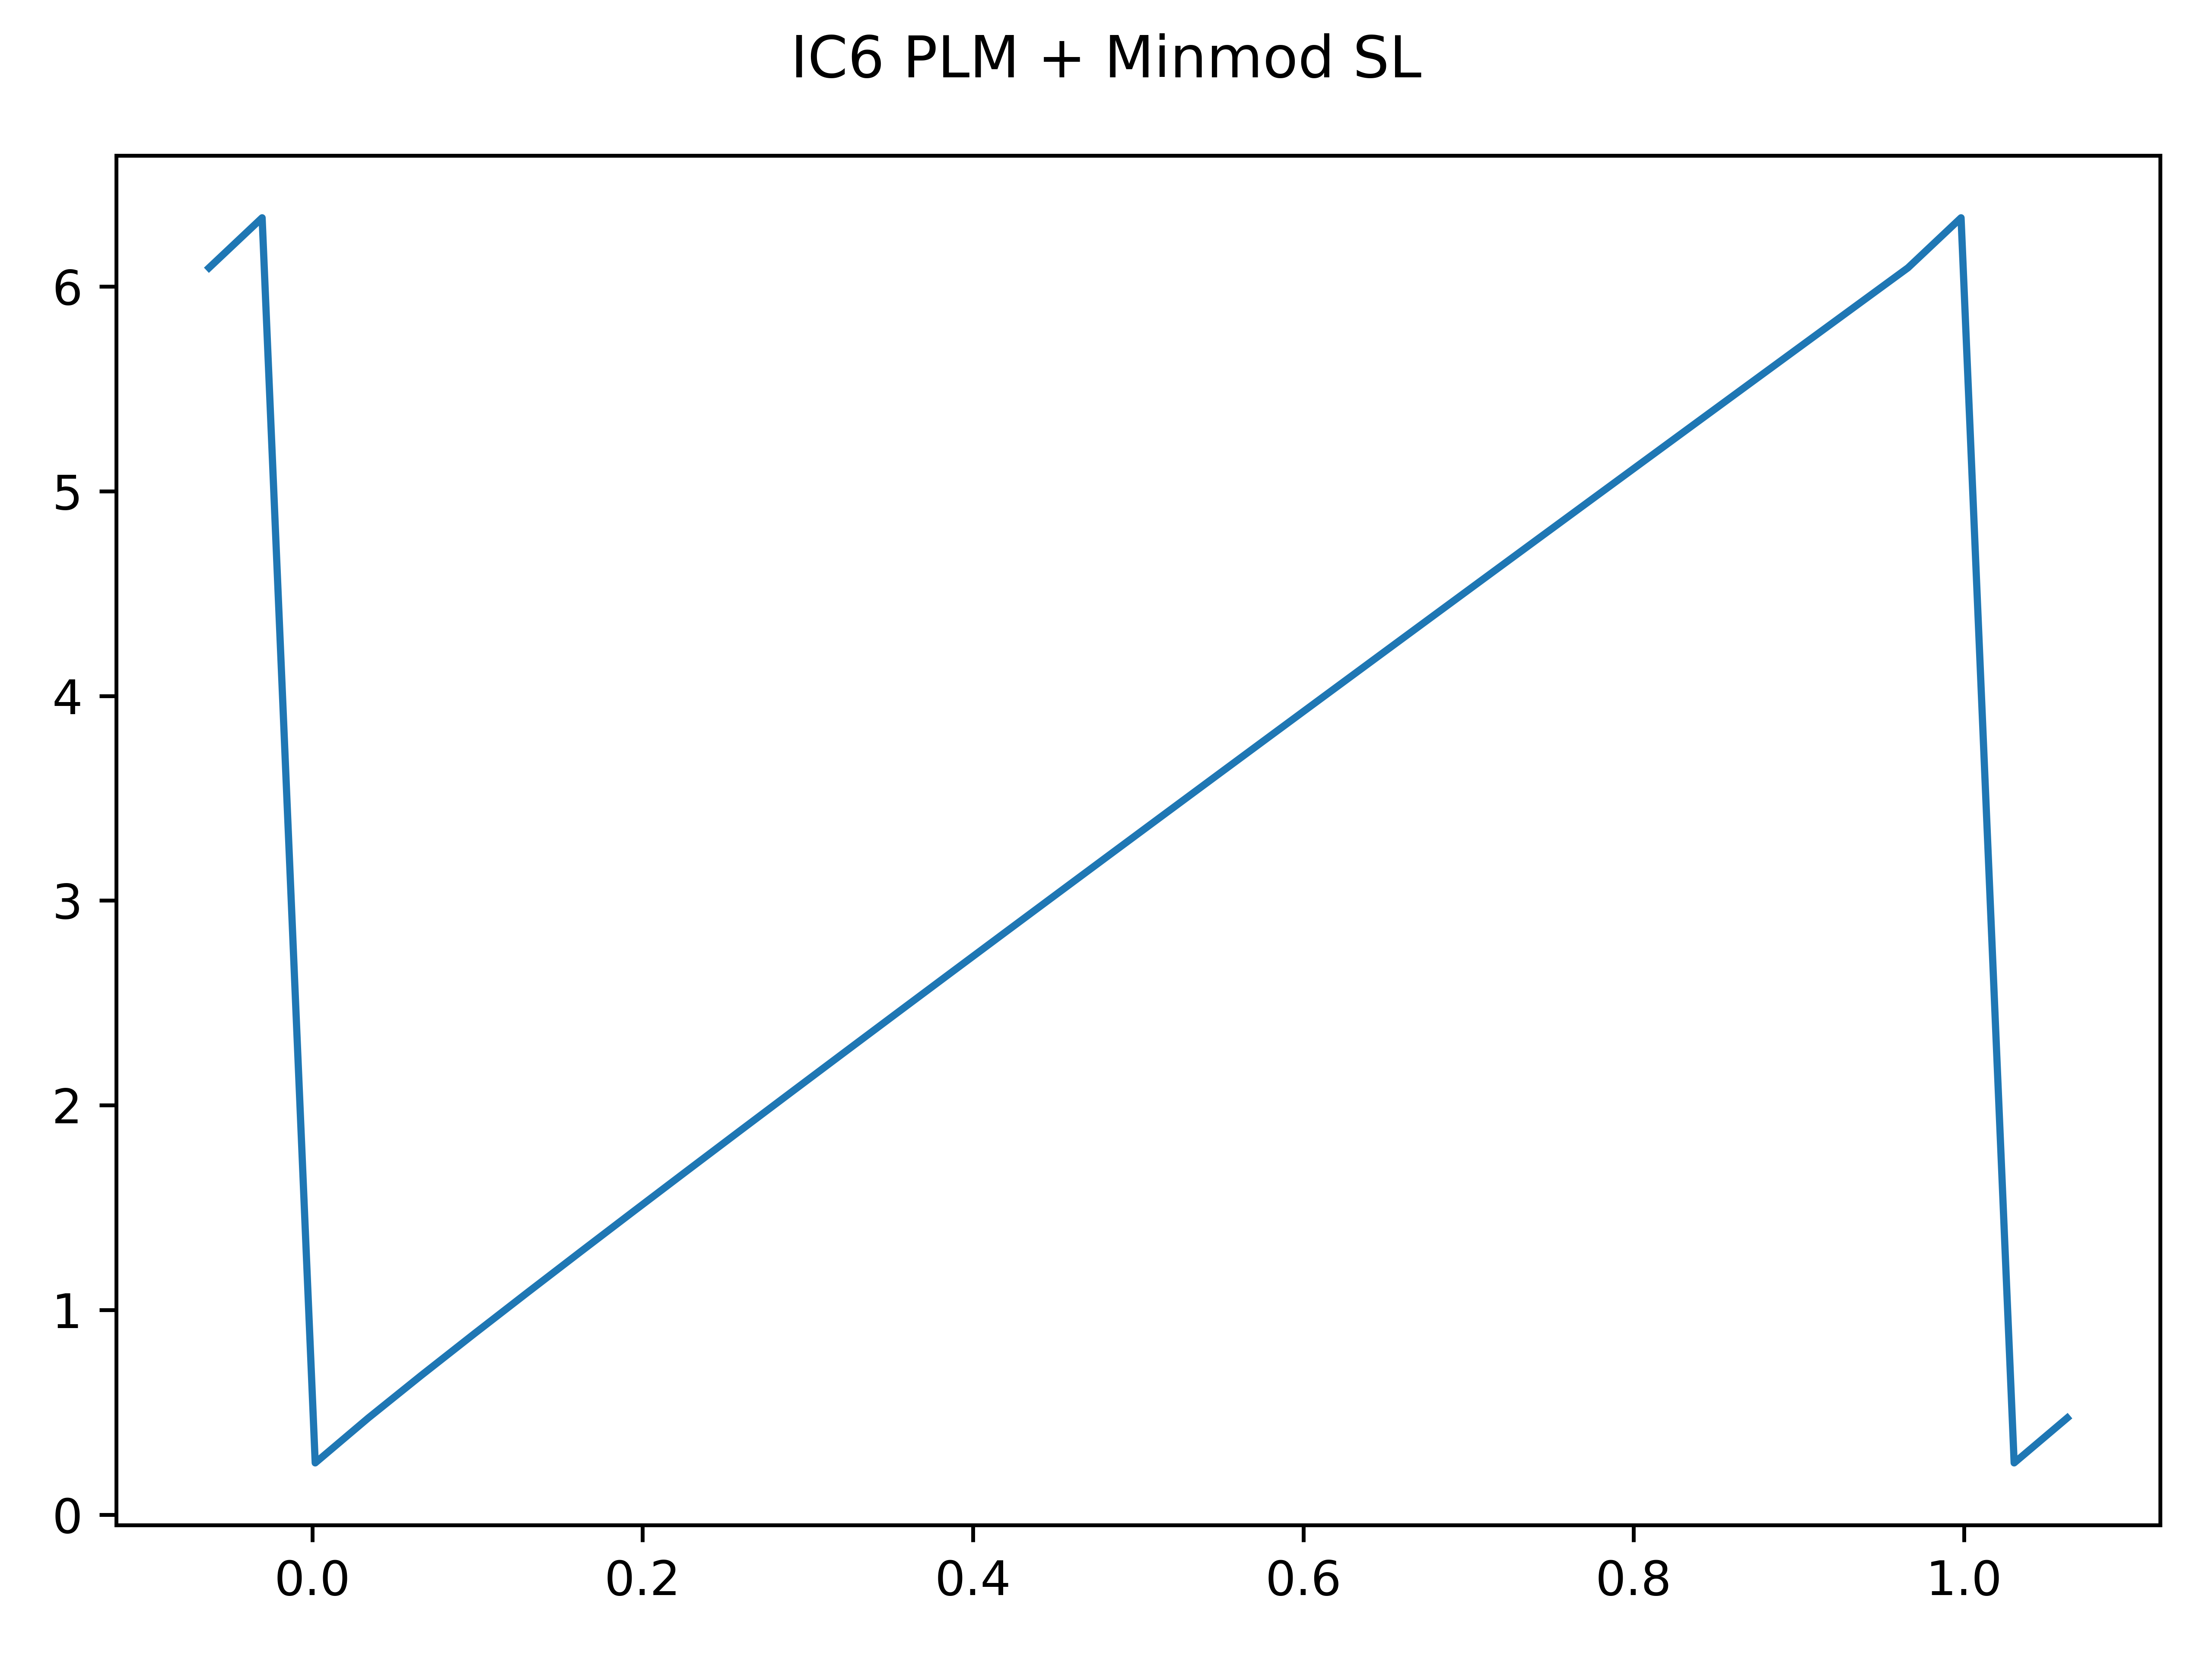
\includegraphics[width=.95\textwidth]{../../code/IC6Methodpm_plot.png}
    \emp
    \bmp{0.25}
        \centering
        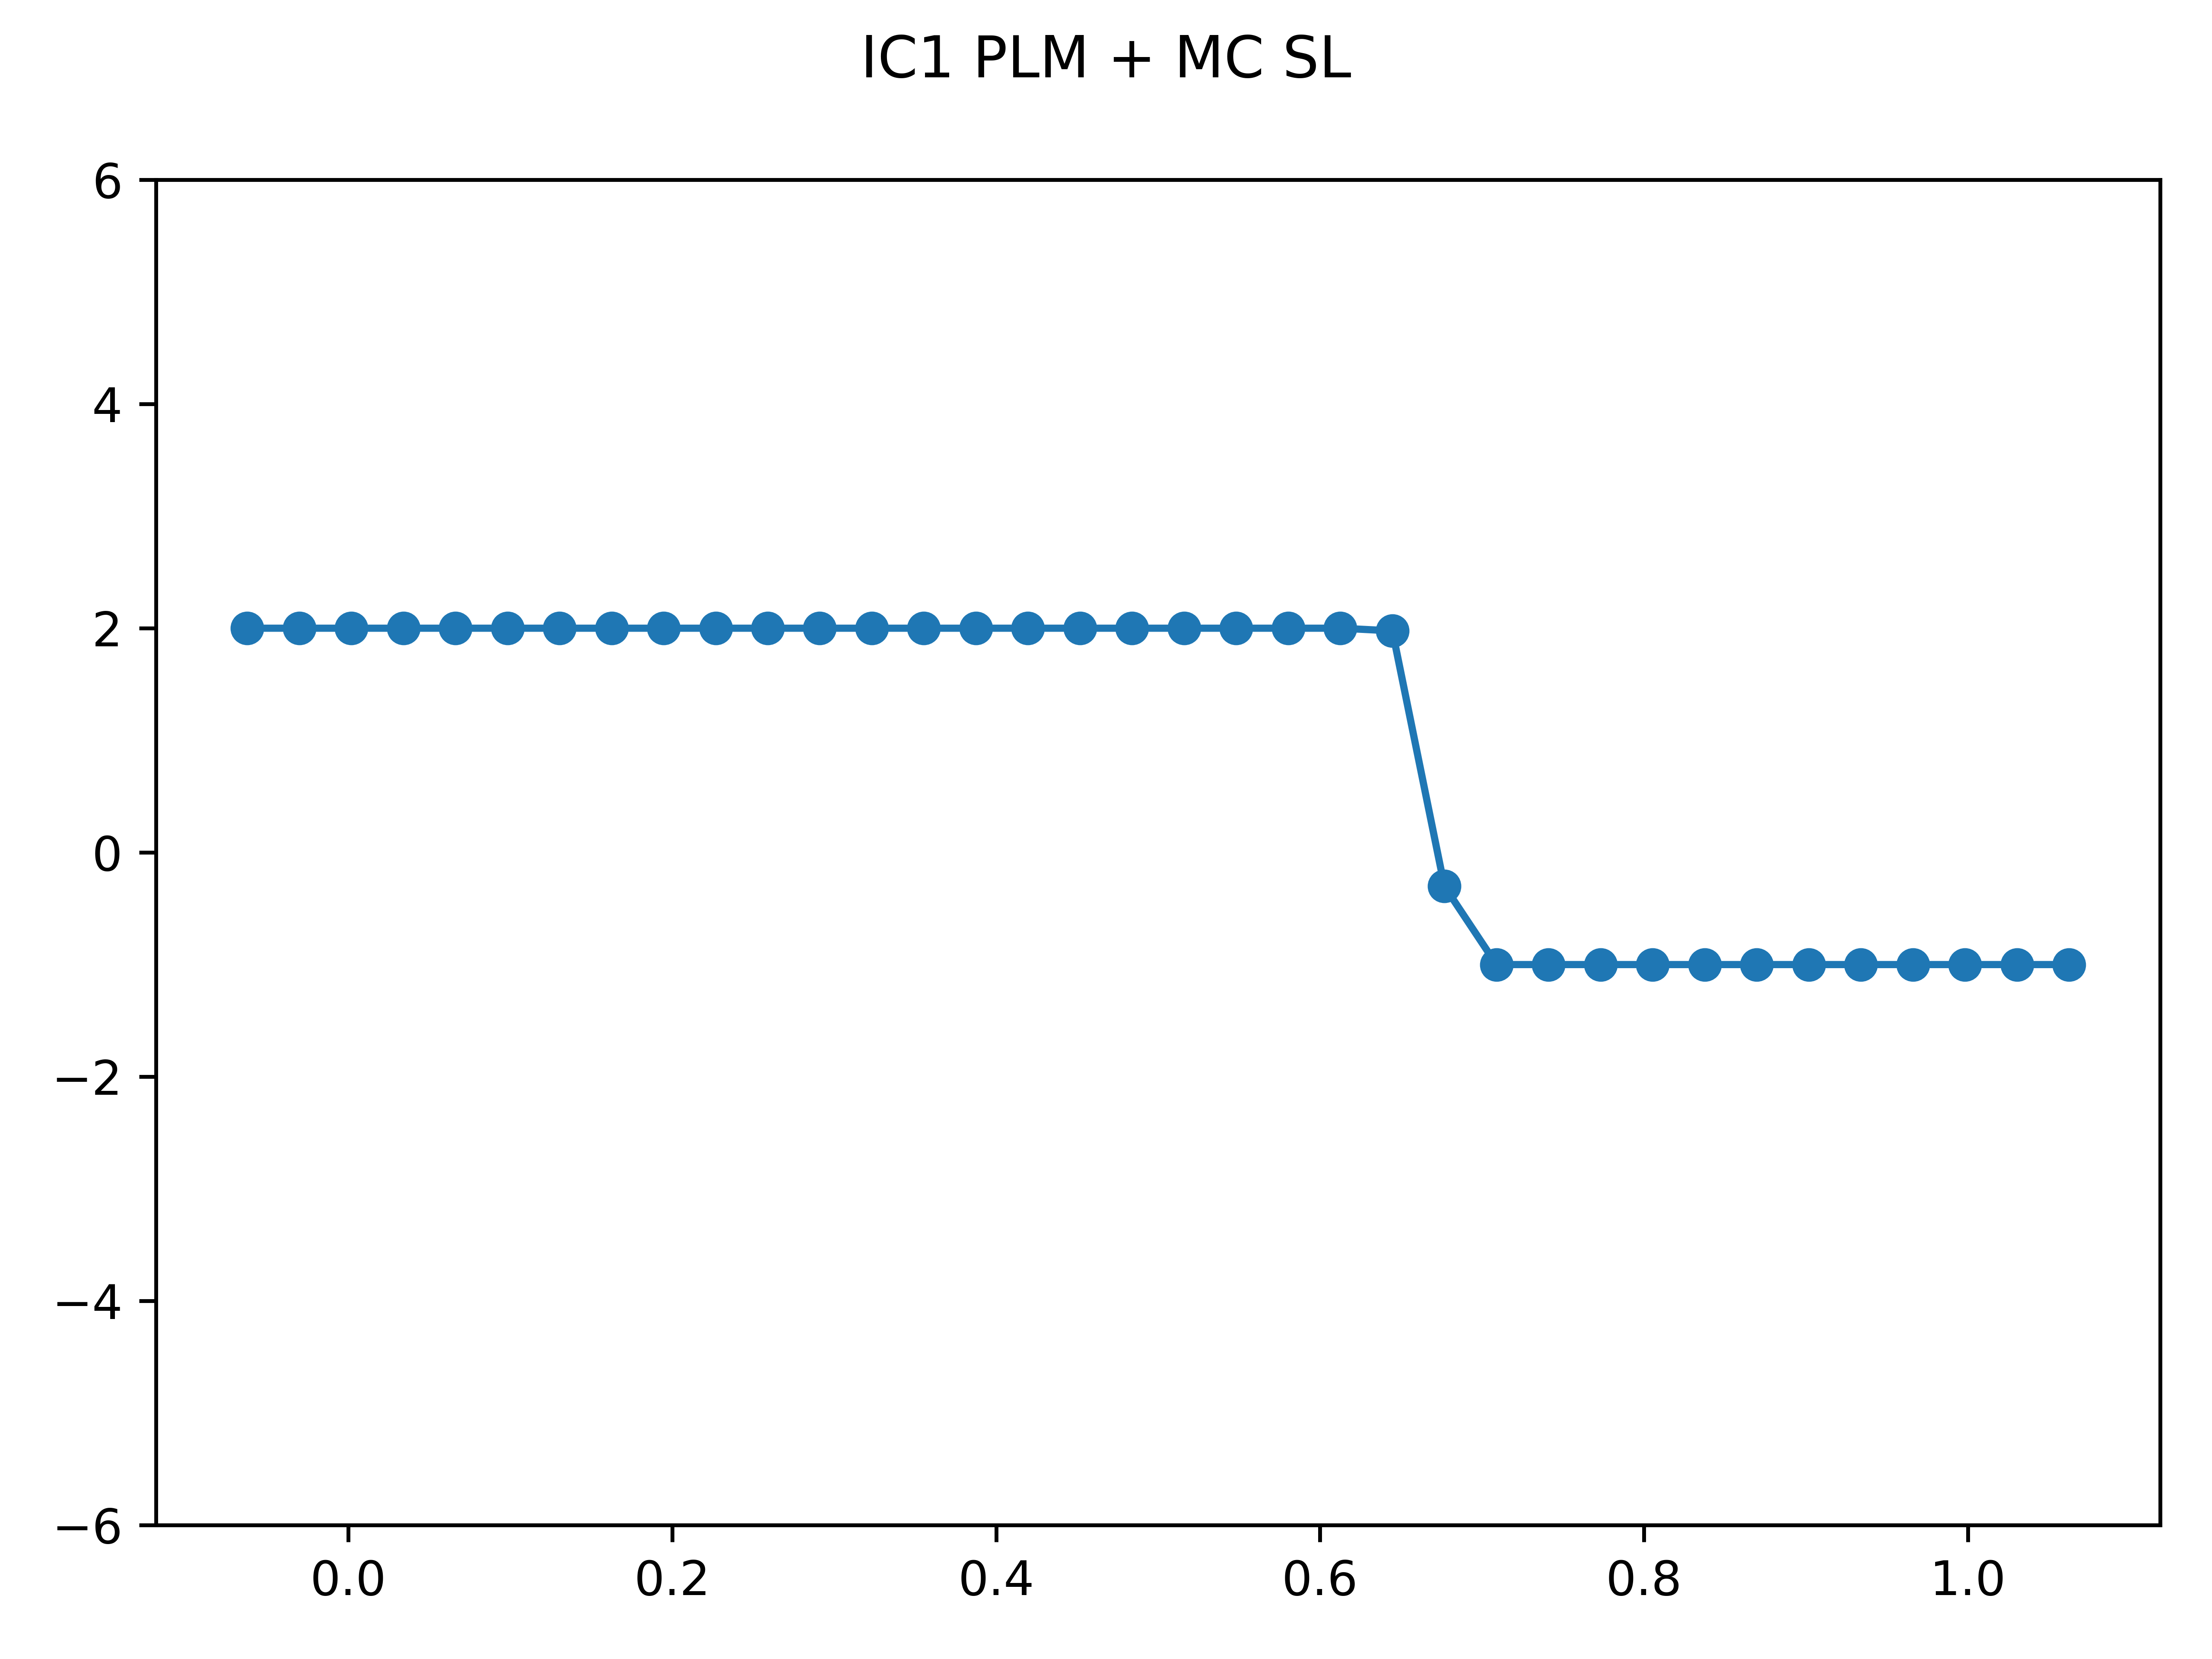
\includegraphics[width=.95\textwidth]{../../code/IC1Methodpo_plot.png}
        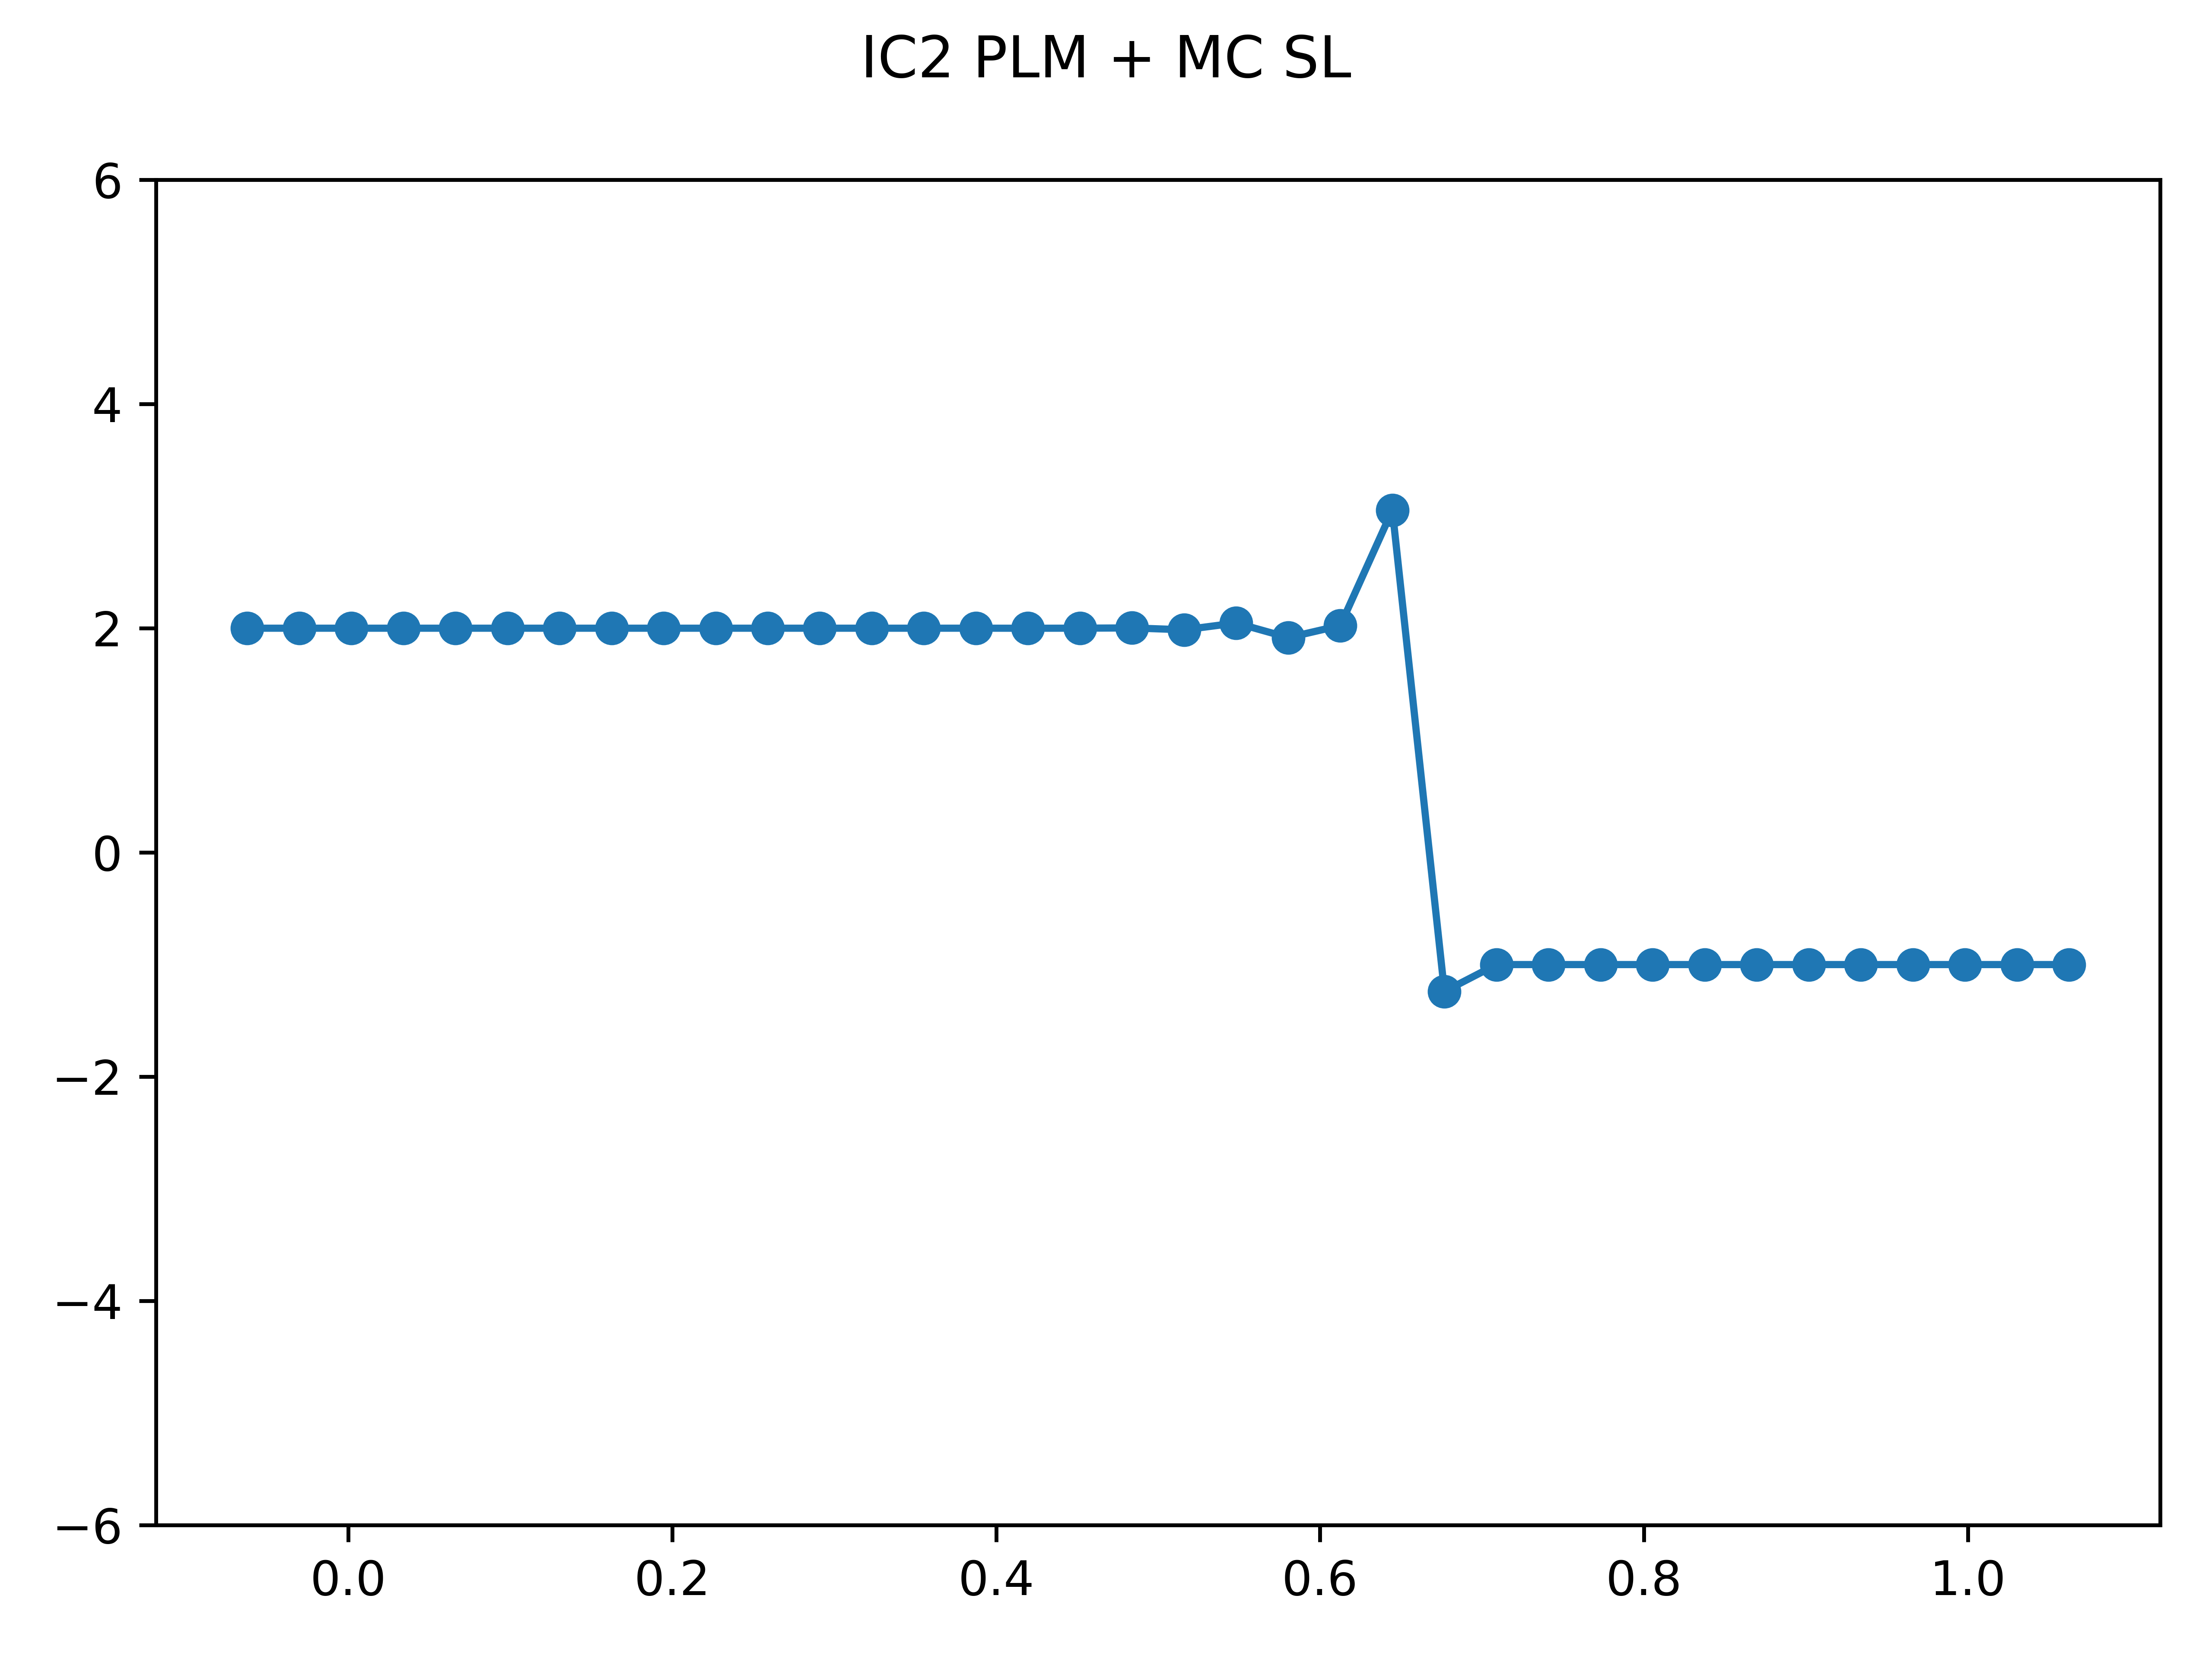
\includegraphics[width=.95\textwidth]{../../code/IC2Methodpo_plot.png}
        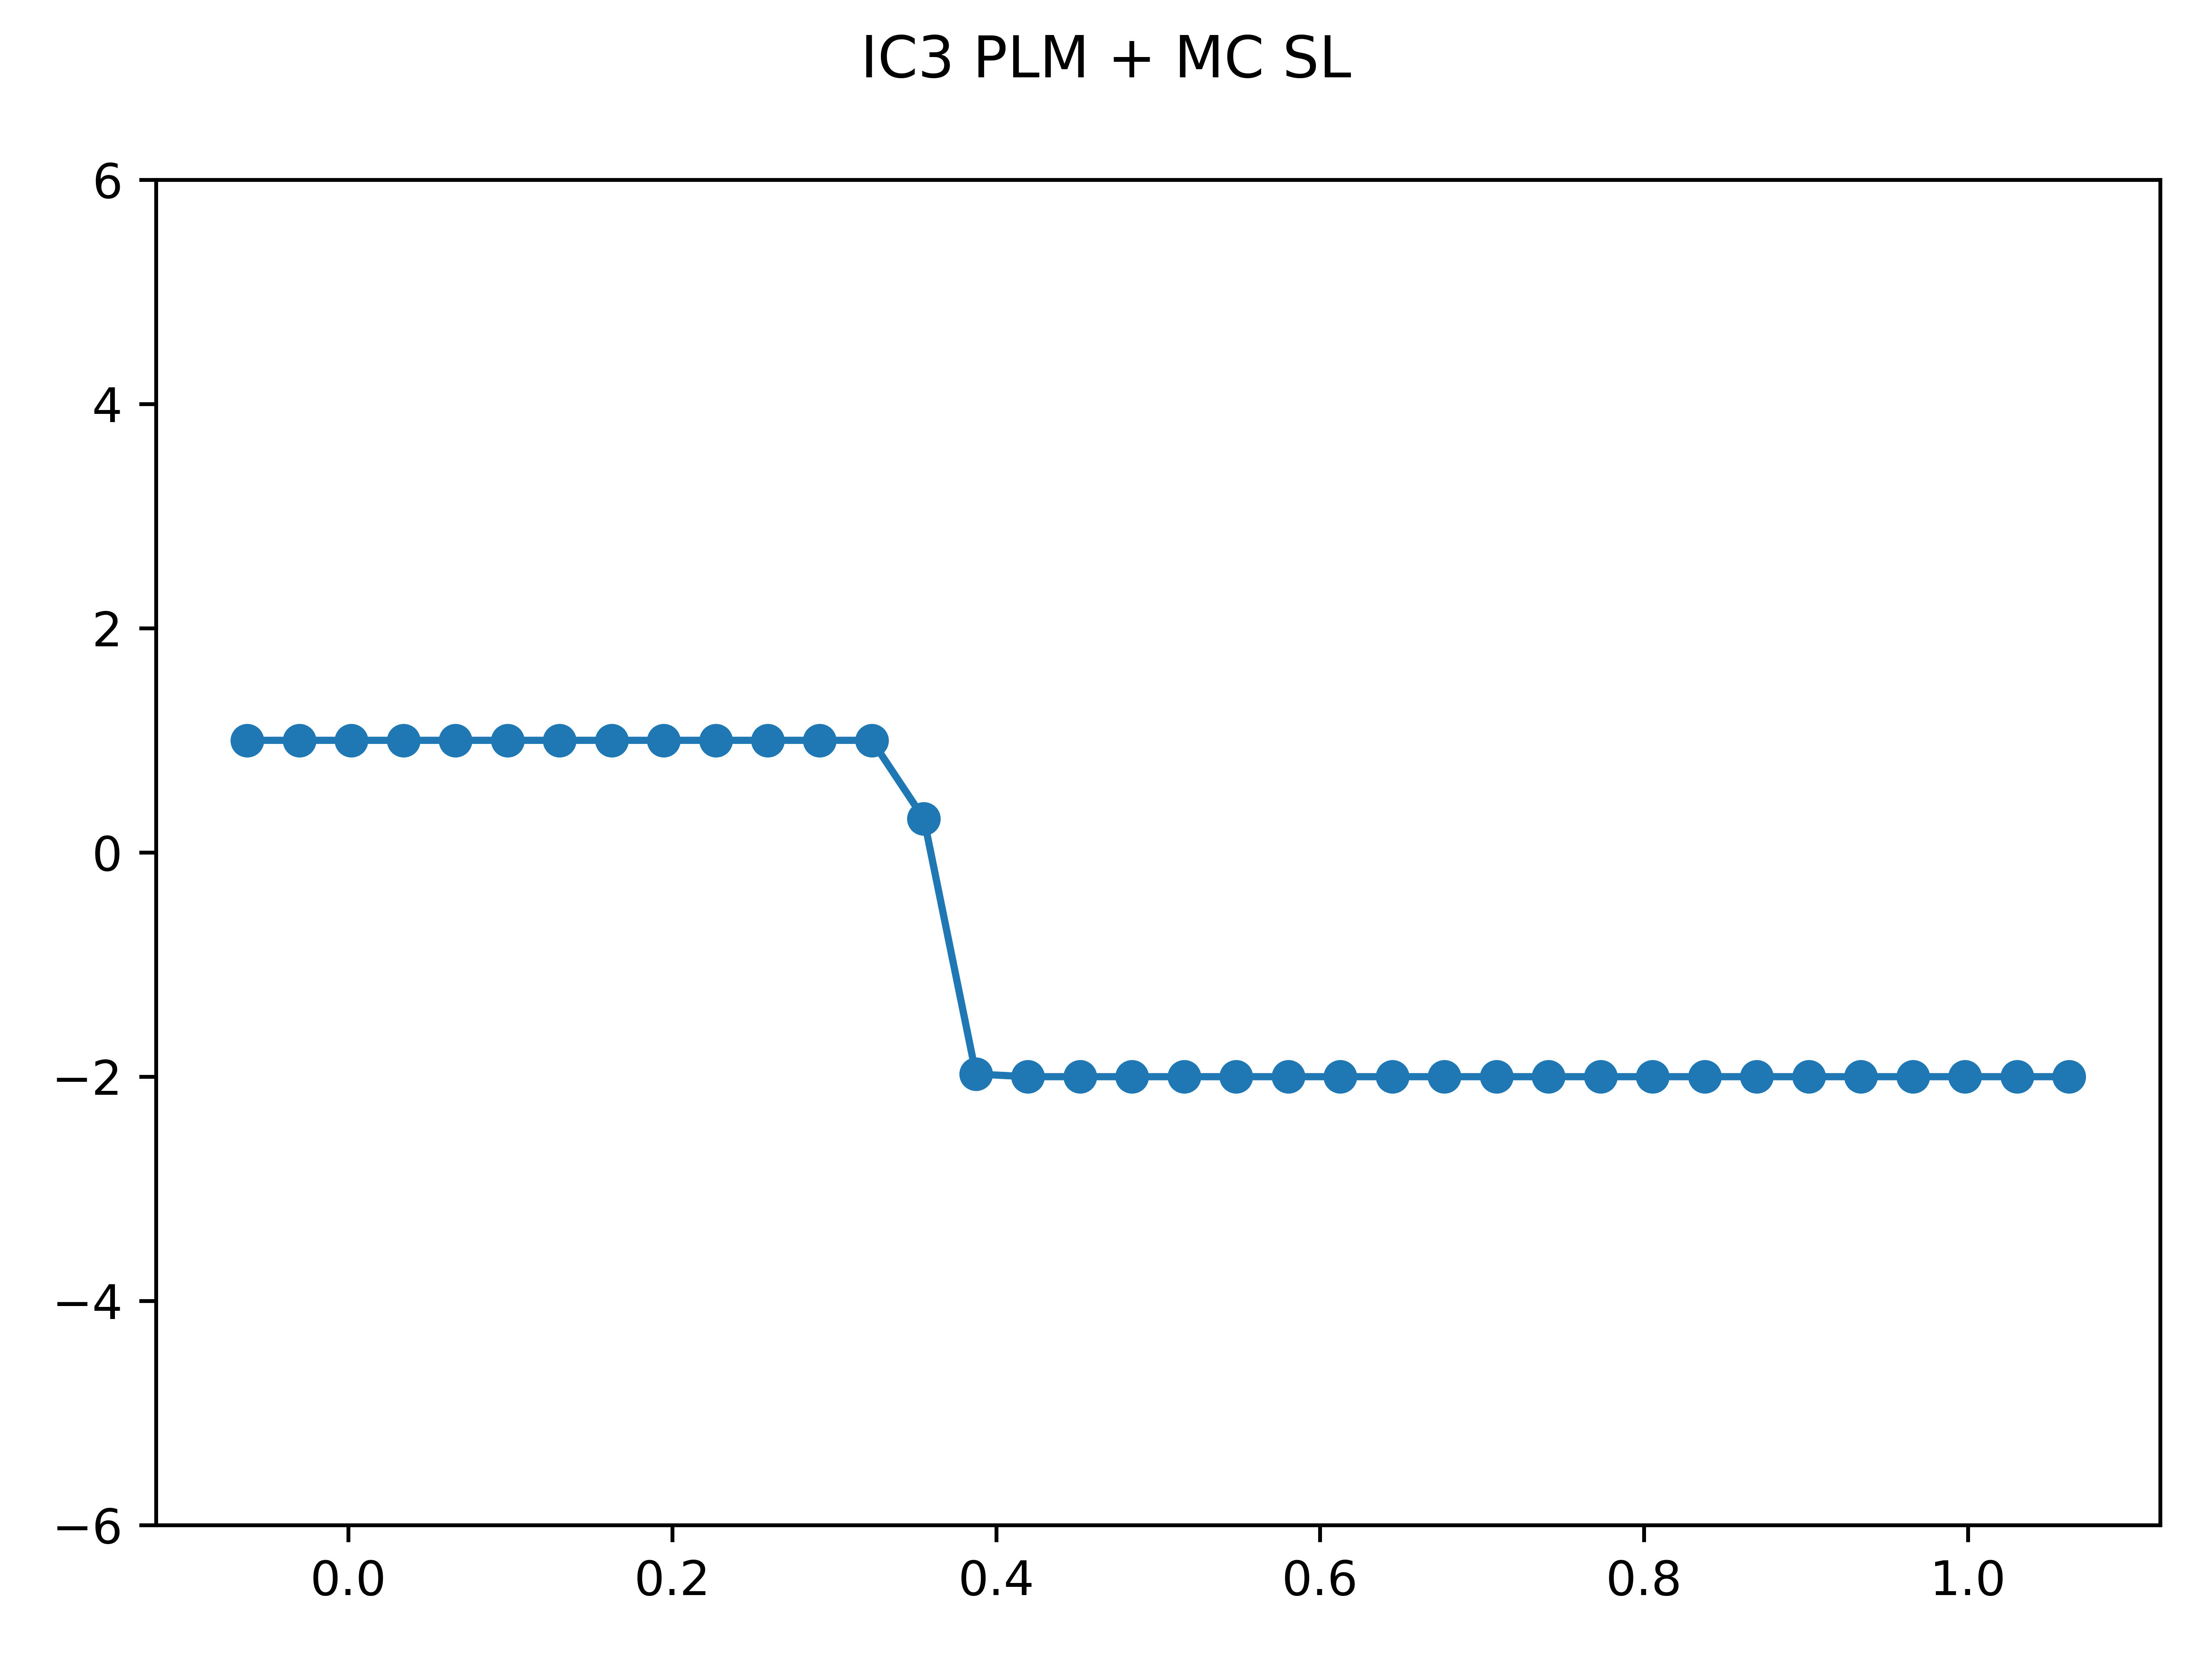
\includegraphics[width=.95\textwidth]{../../code/IC3Methodpo_plot.png}
        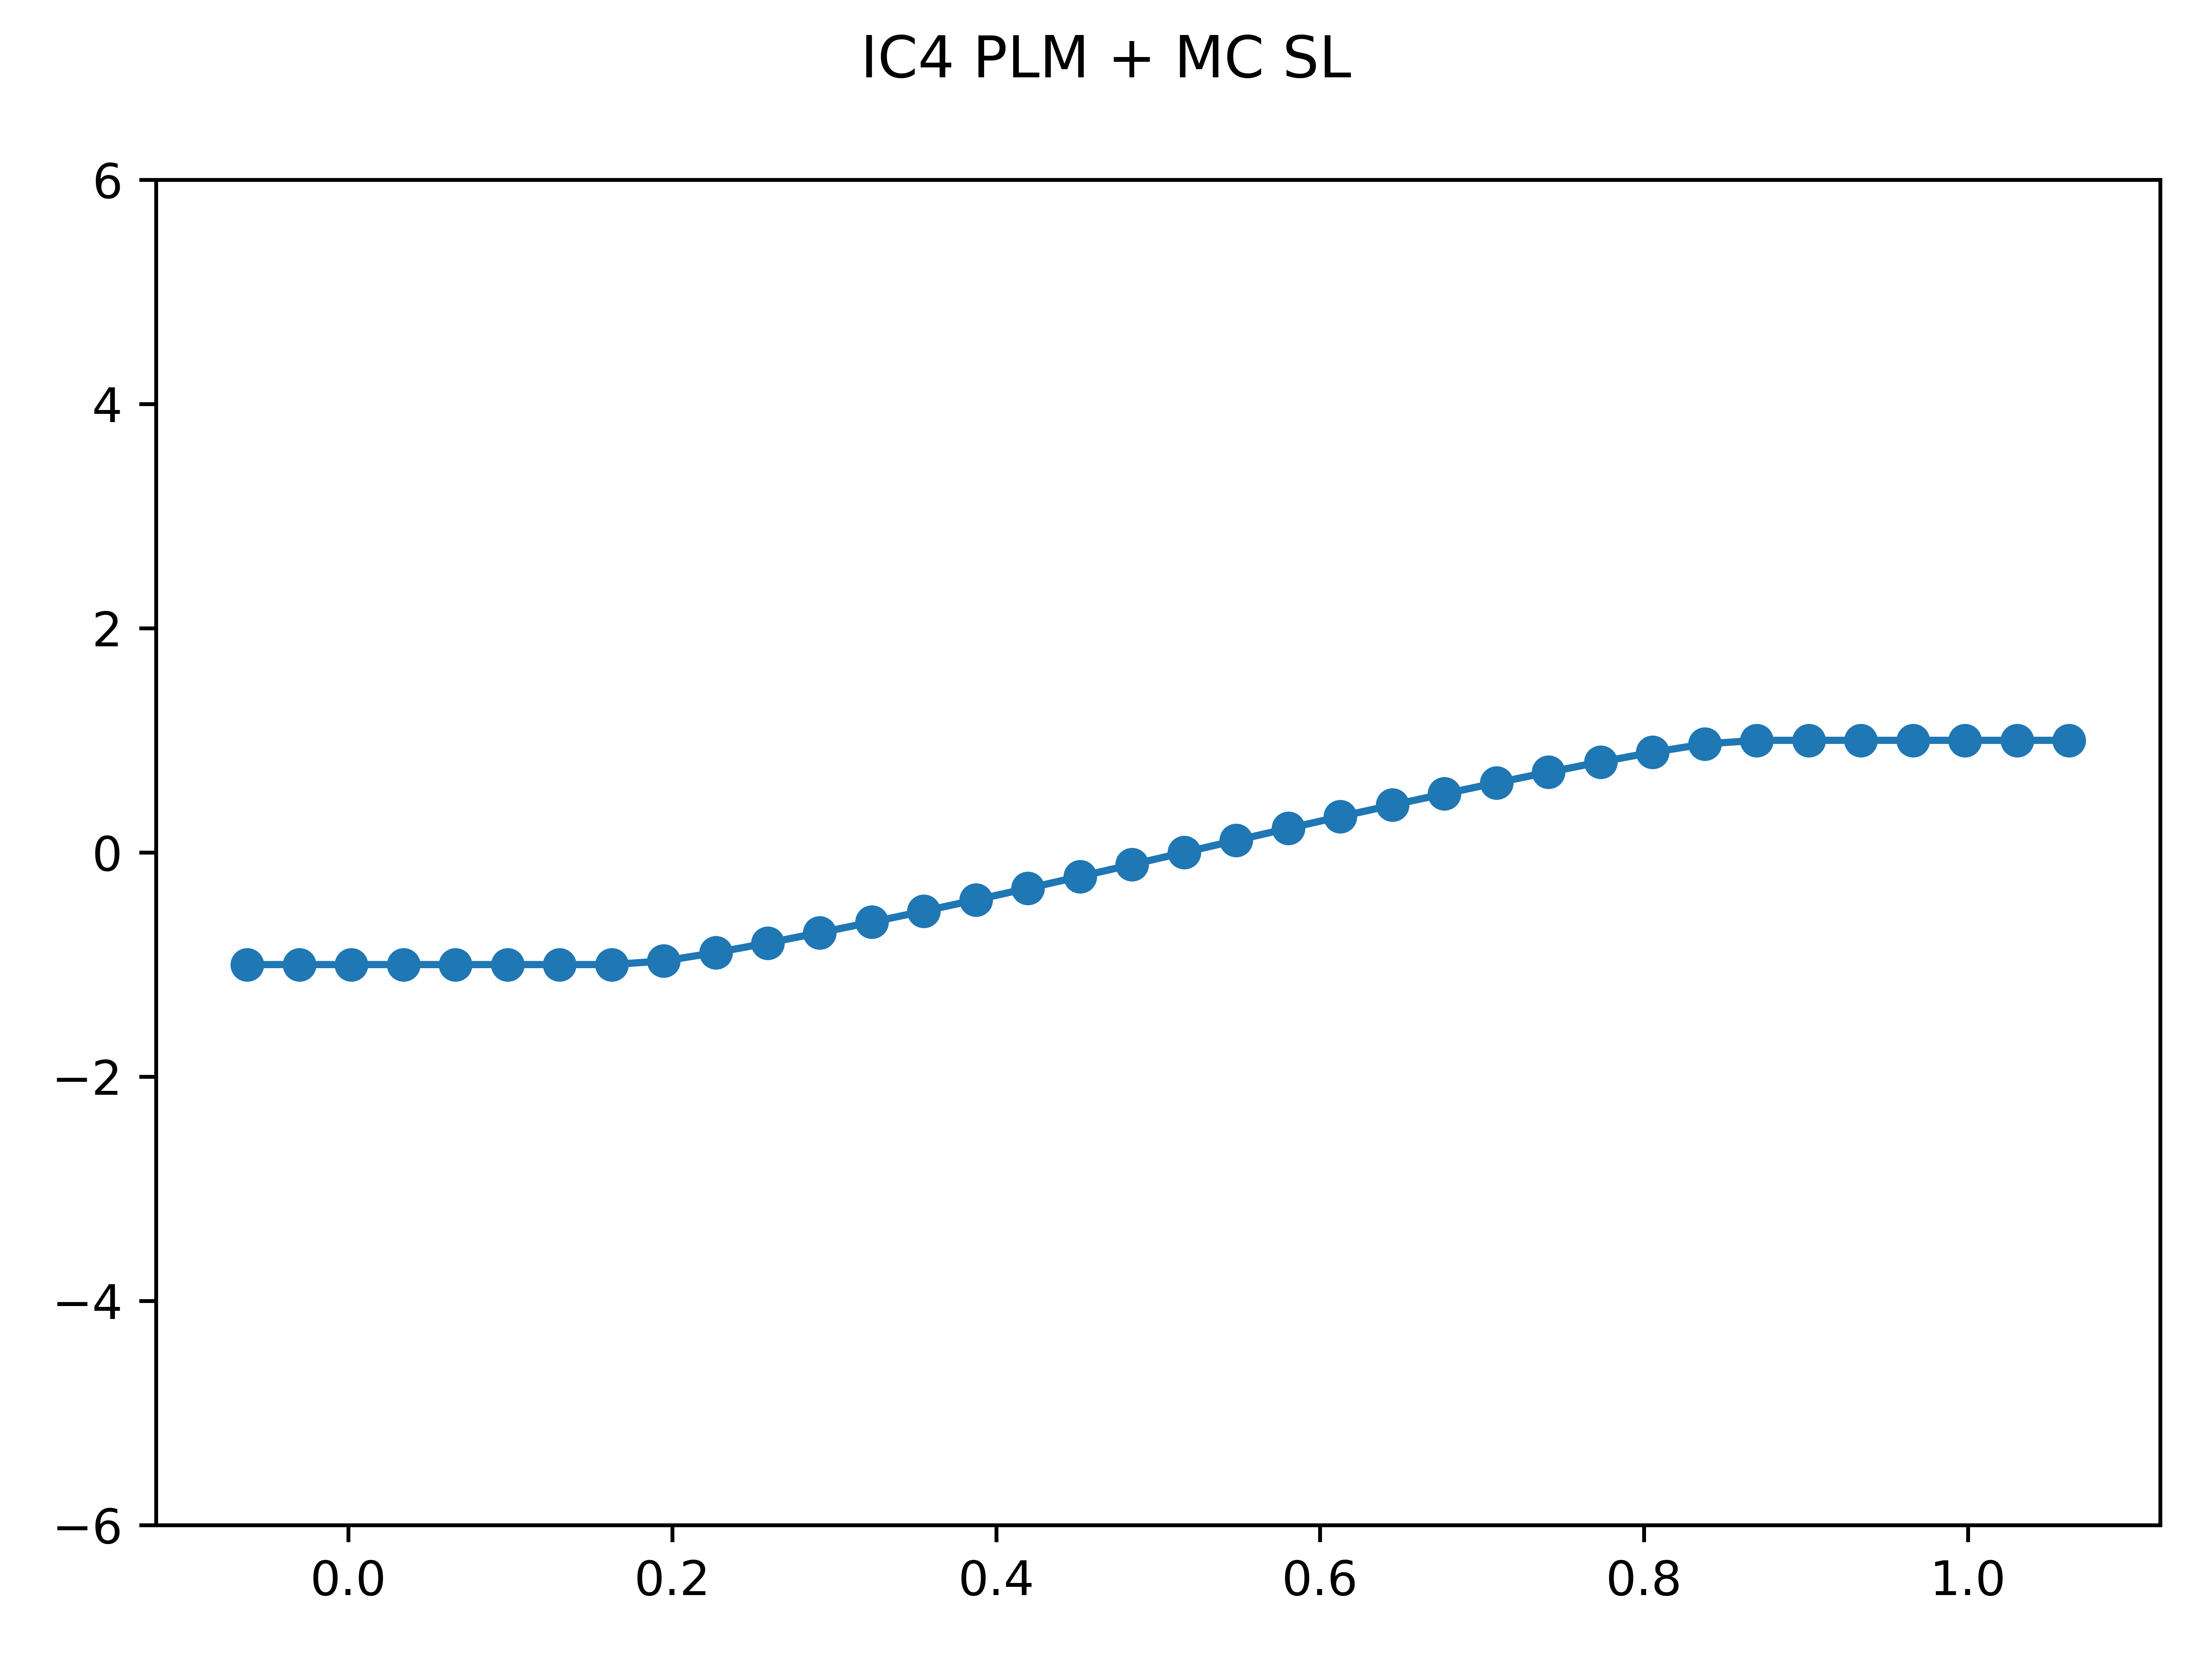
\includegraphics[width=.95\textwidth]{../../code/IC4Methodpo_plot.png}
        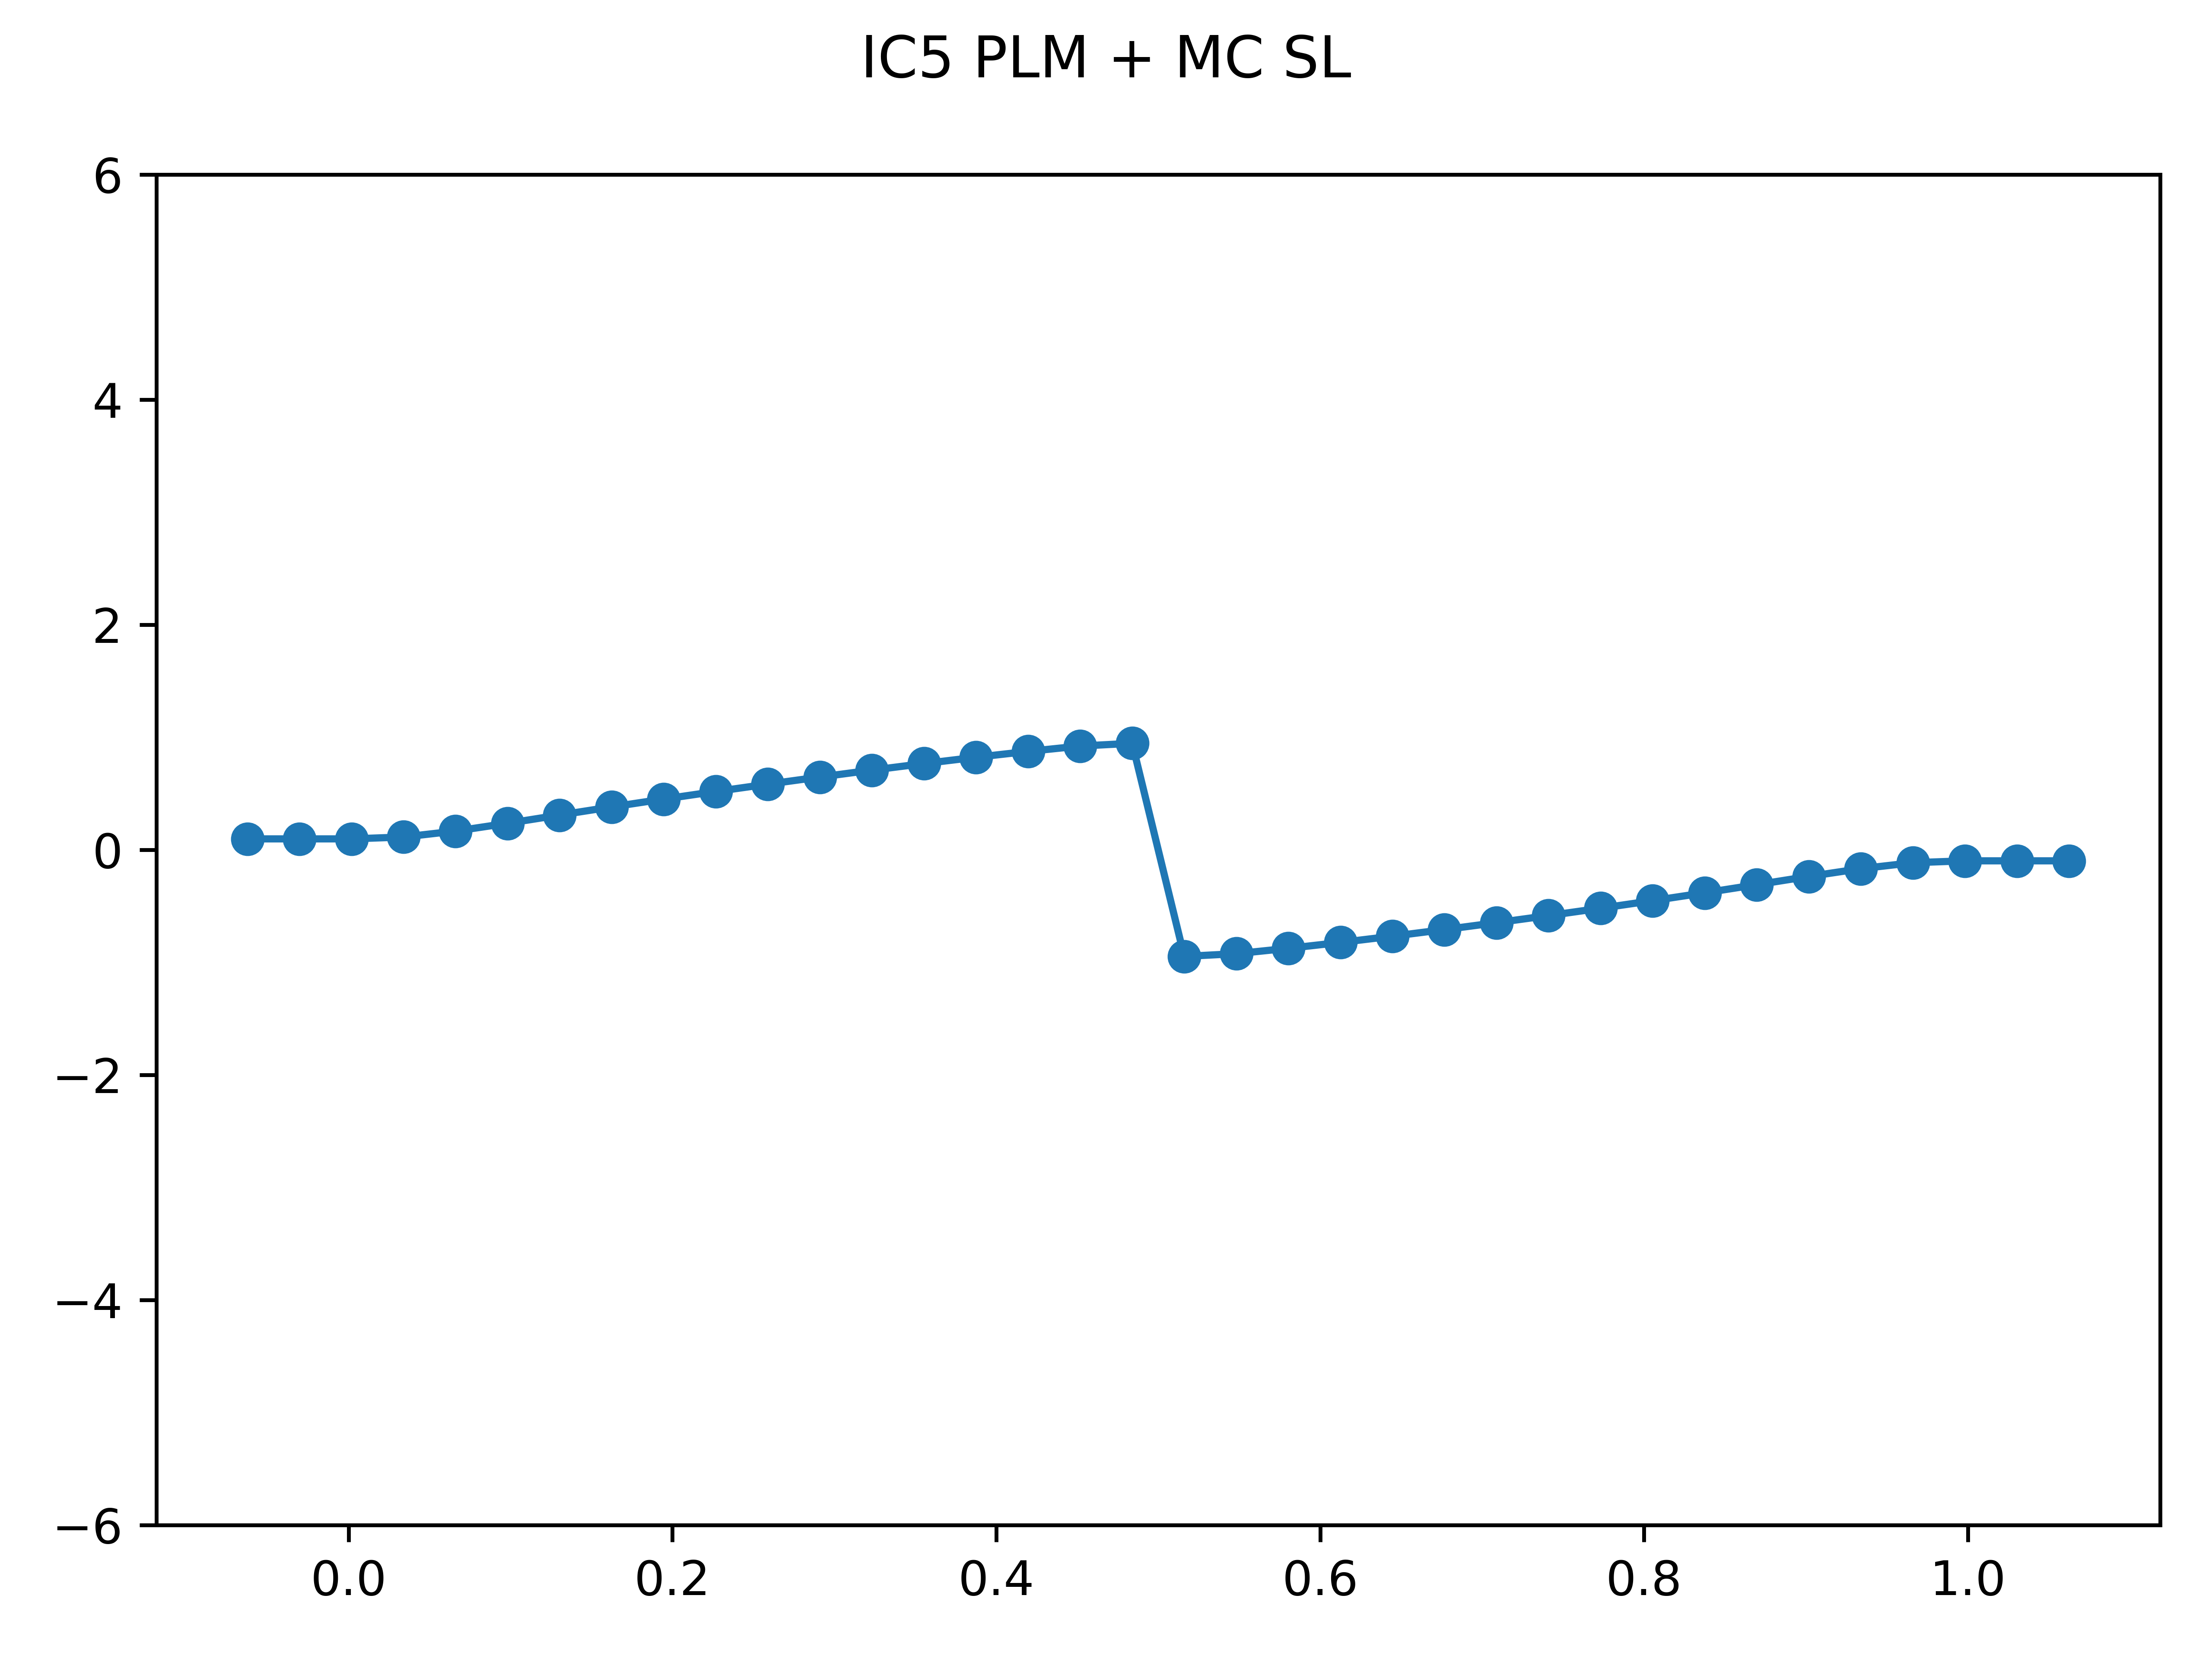
\includegraphics[width=.95\textwidth]{../../code/IC5Methodpo_plot.png}
        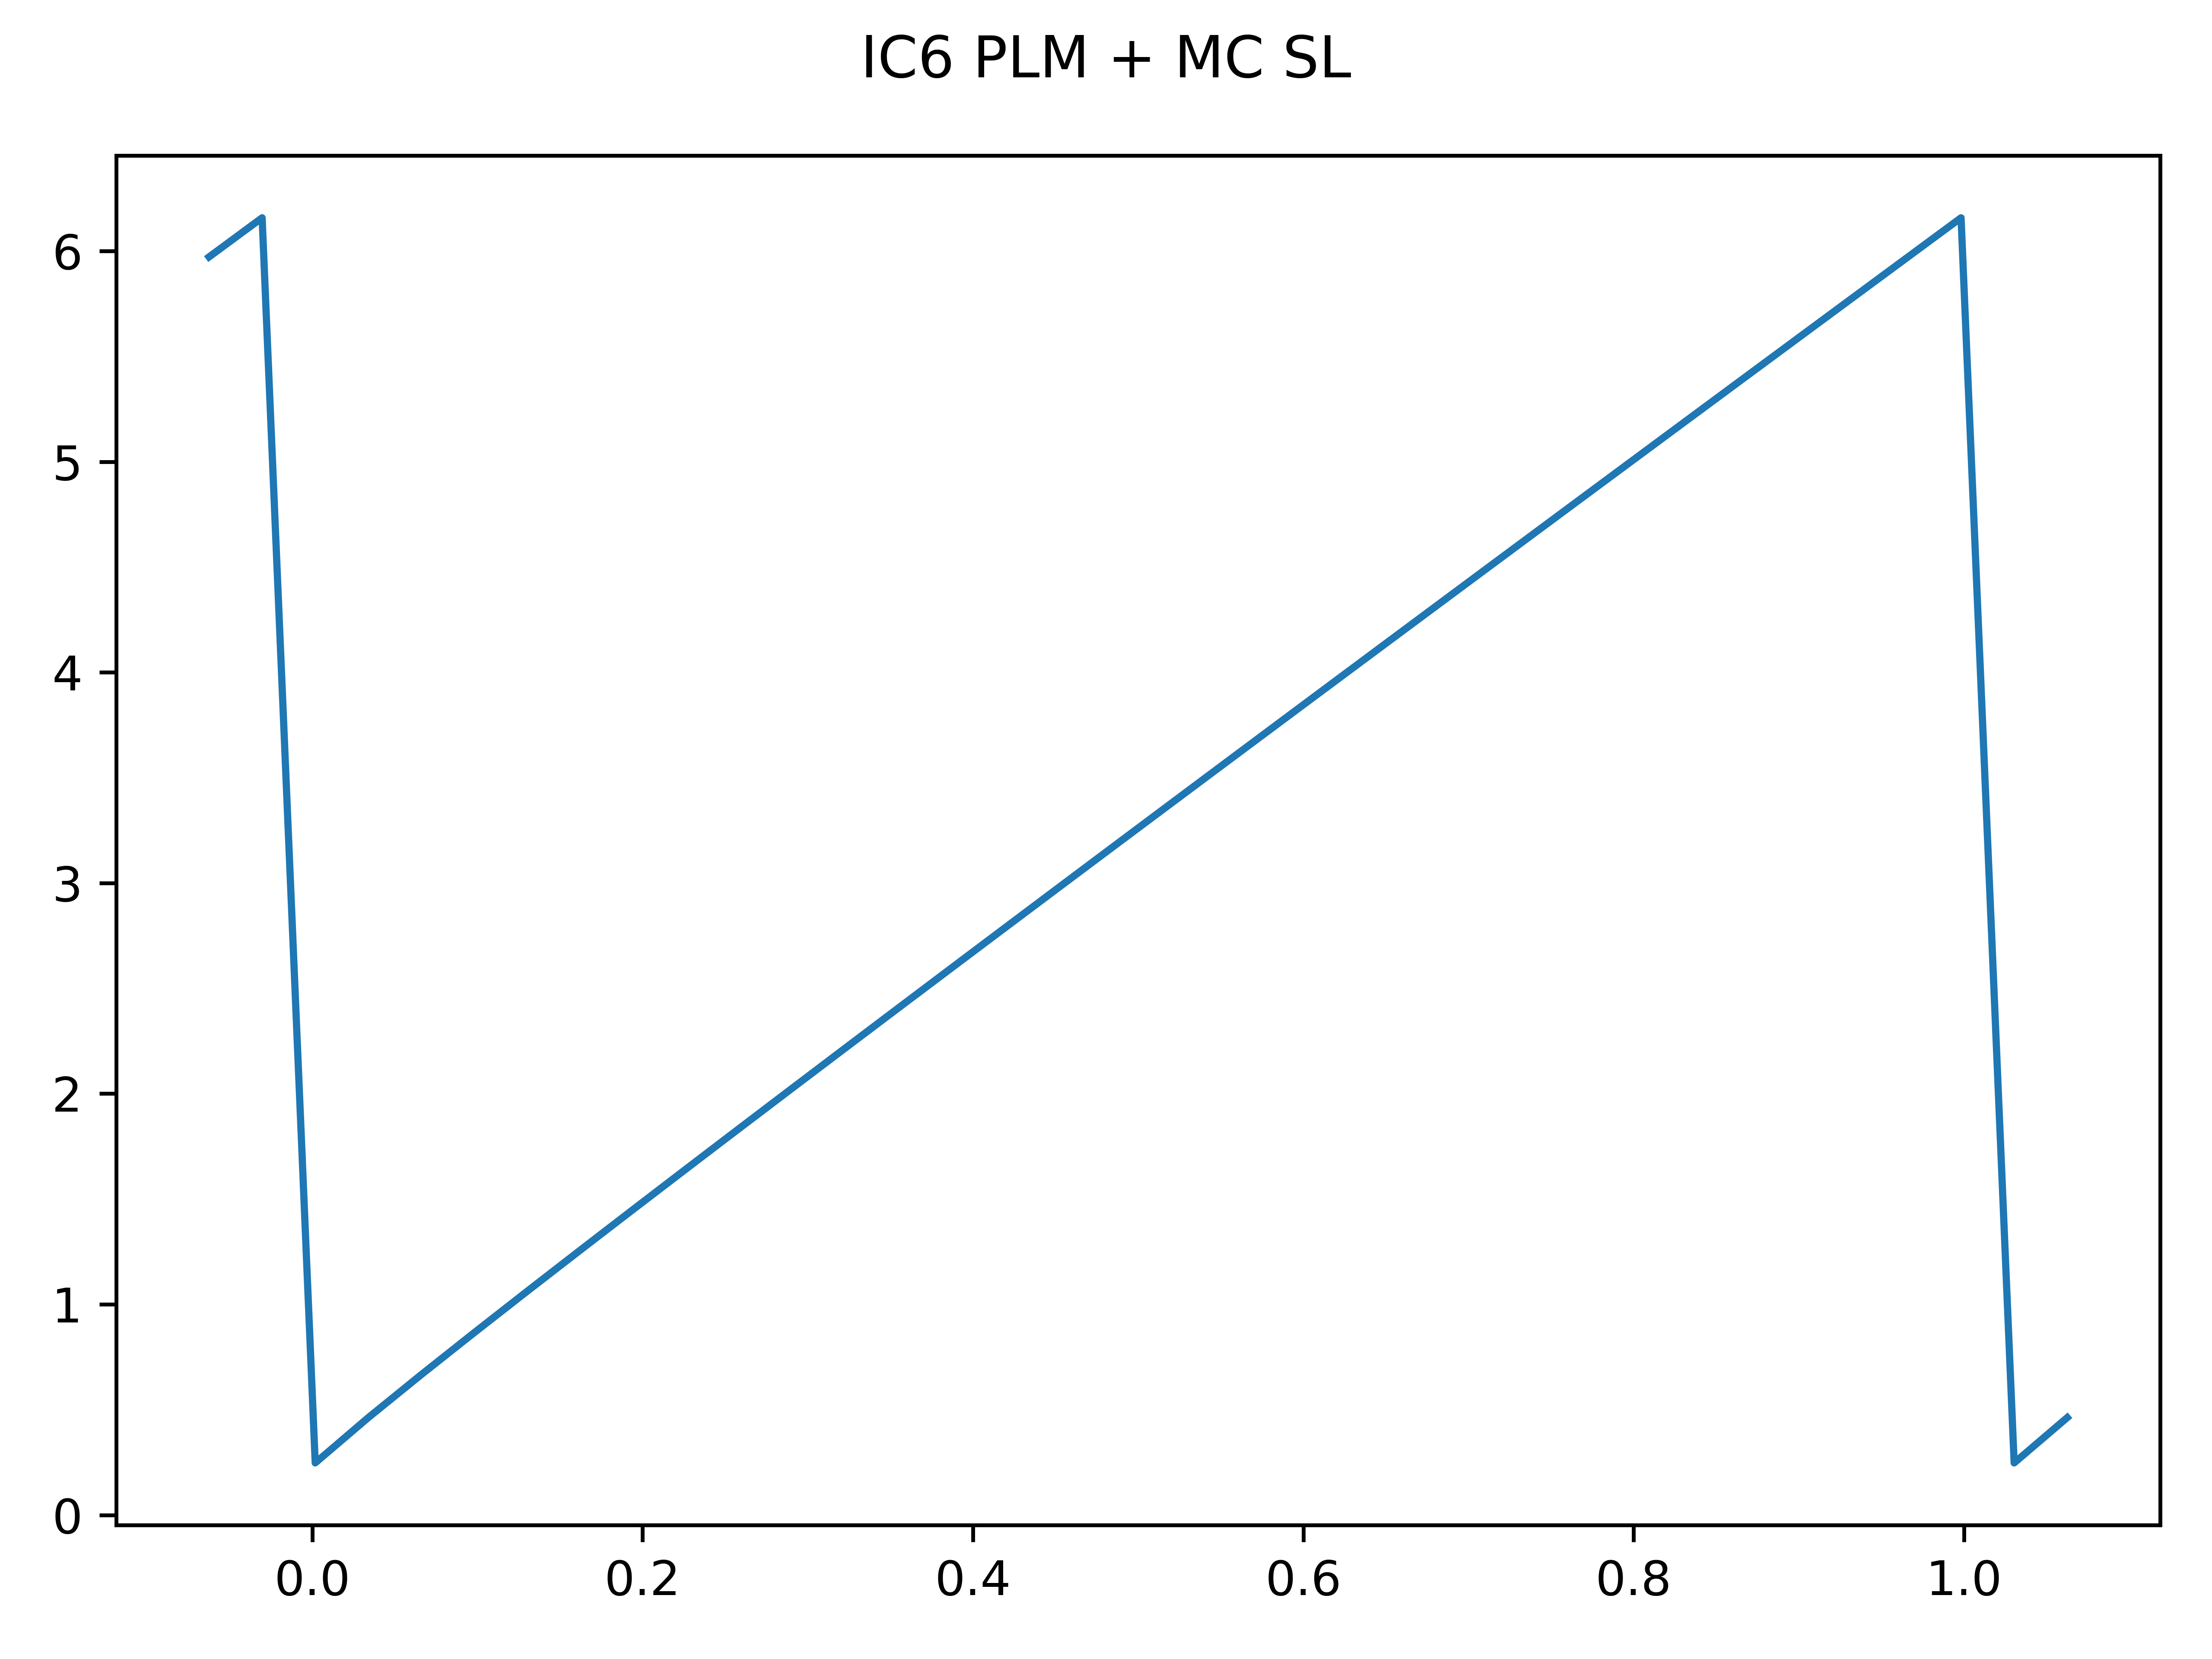
\includegraphics[width=.95\textwidth]{../../code/IC6Methodpo_plot.png}
    \emp
    \bmp{0.25}
        \centering
        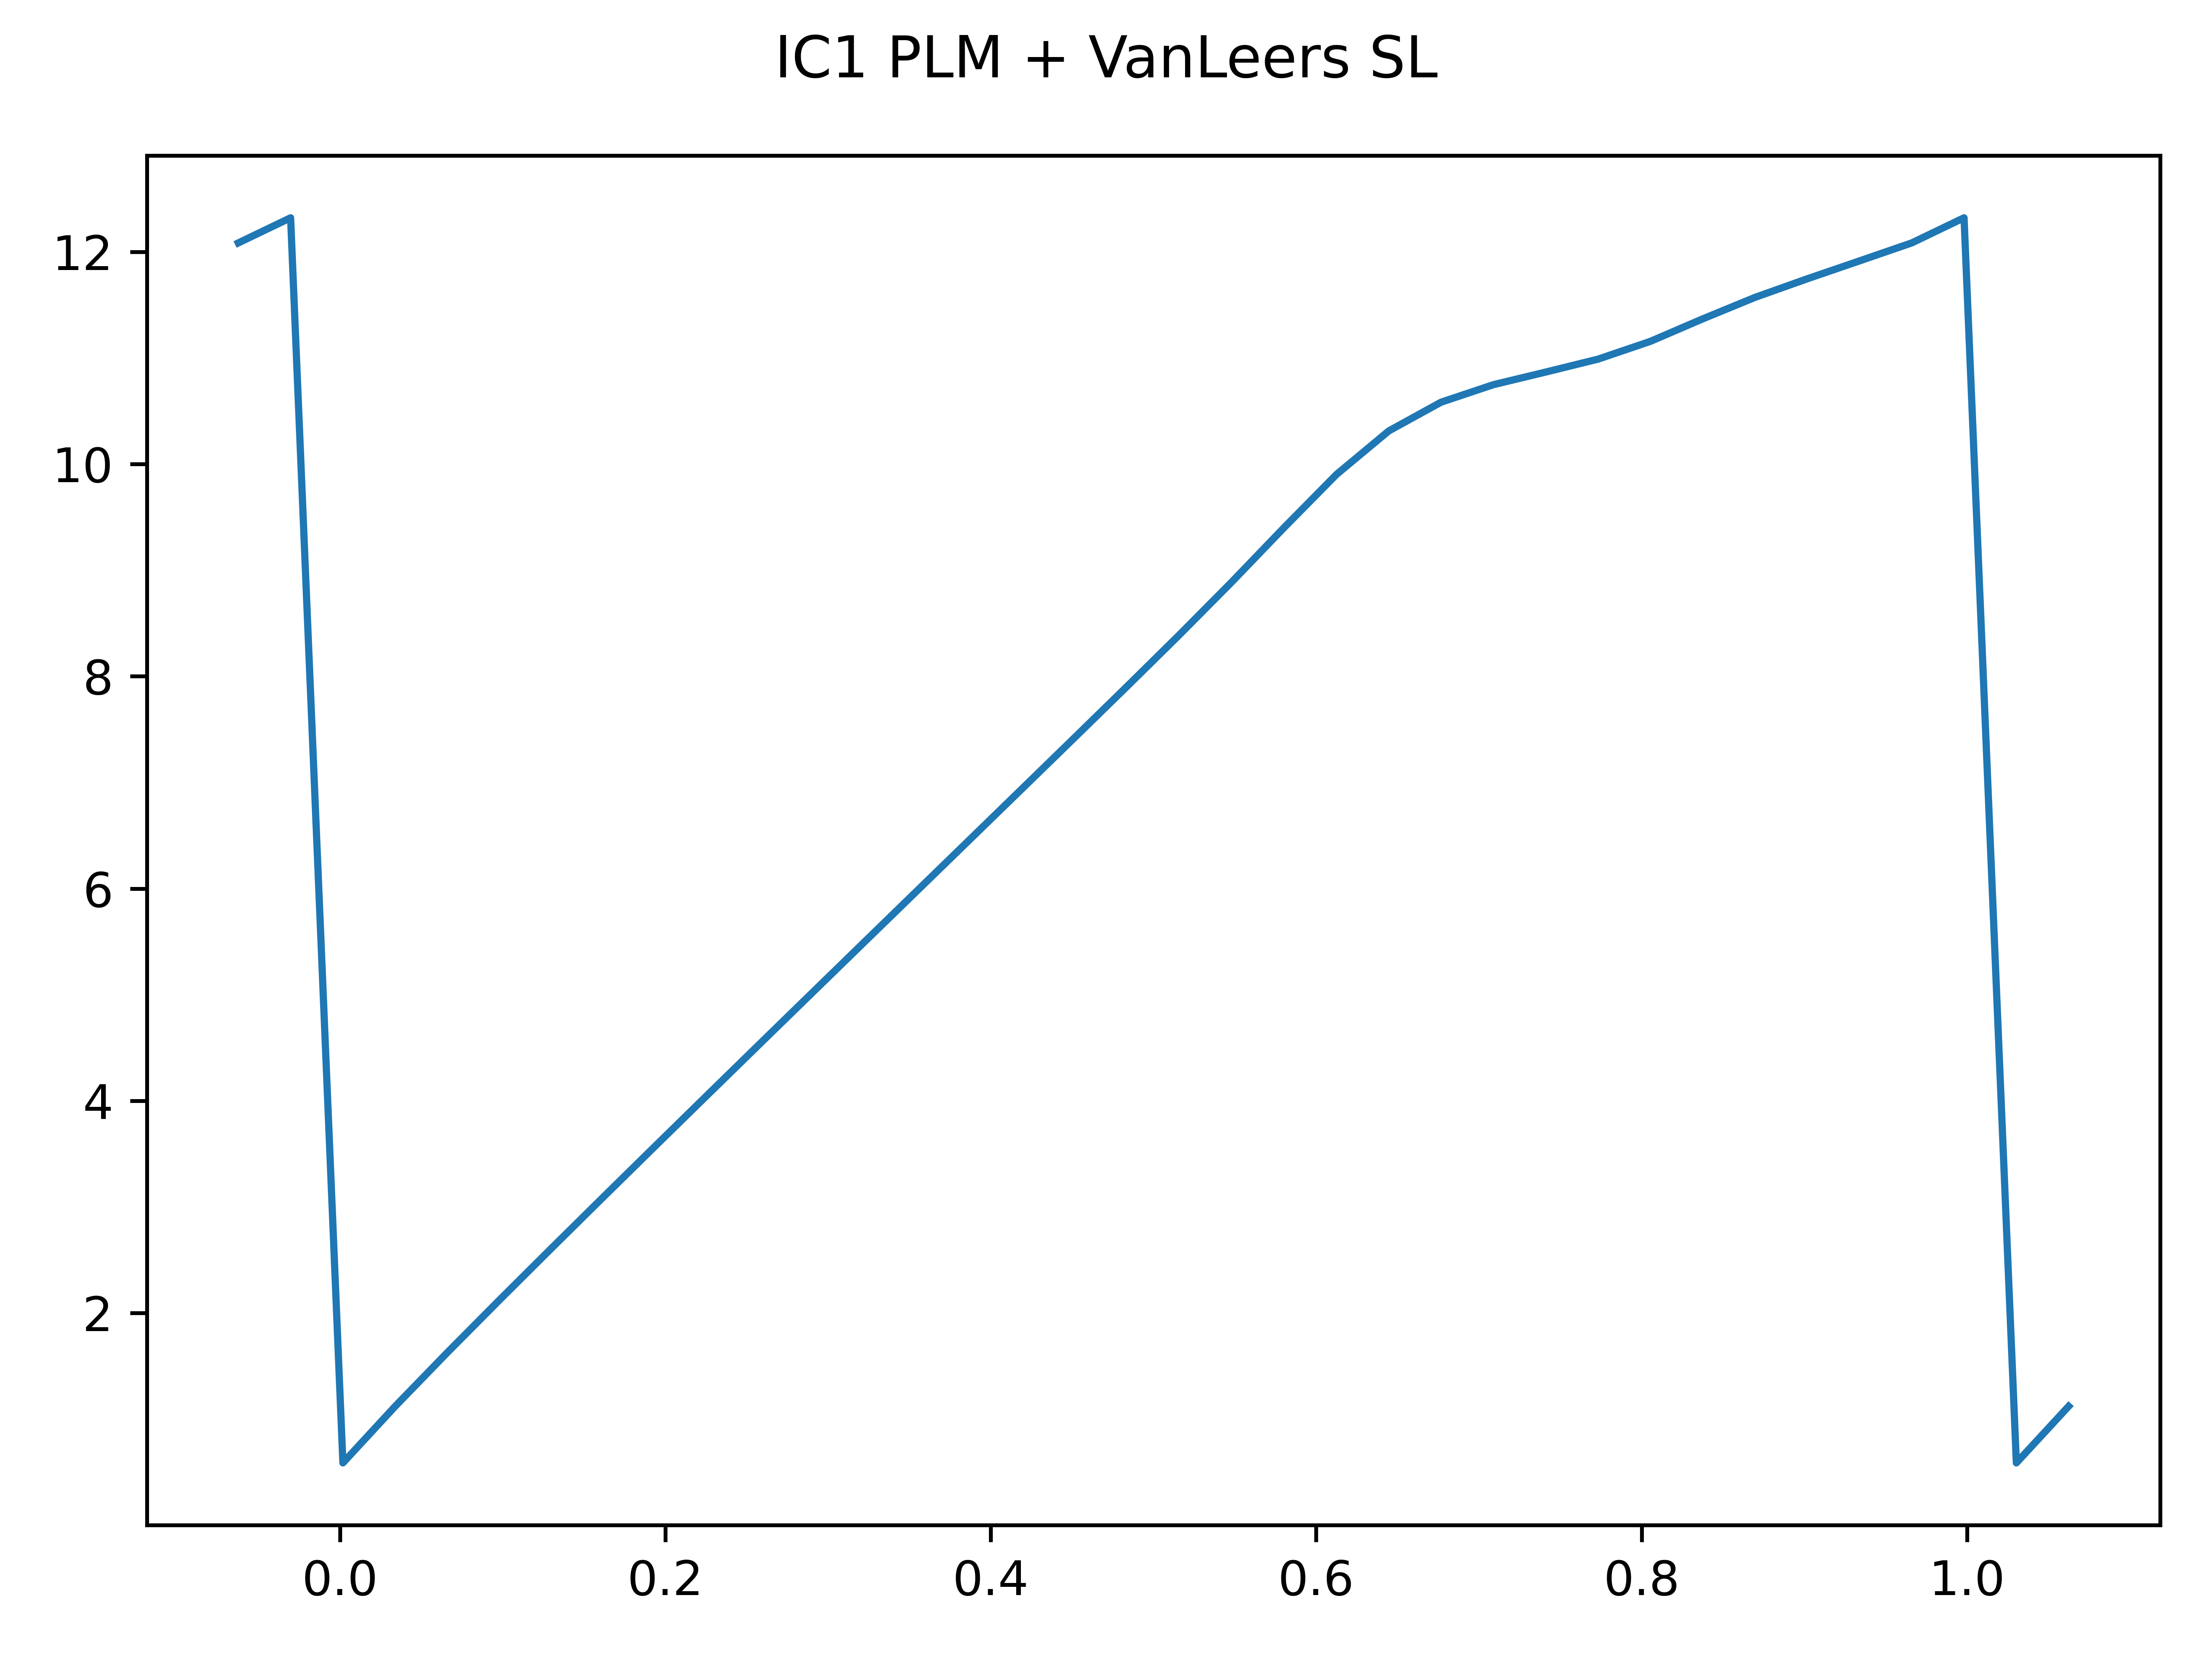
\includegraphics[width=.95\textwidth]{../../code/IC1Methodpv_plot.png}
        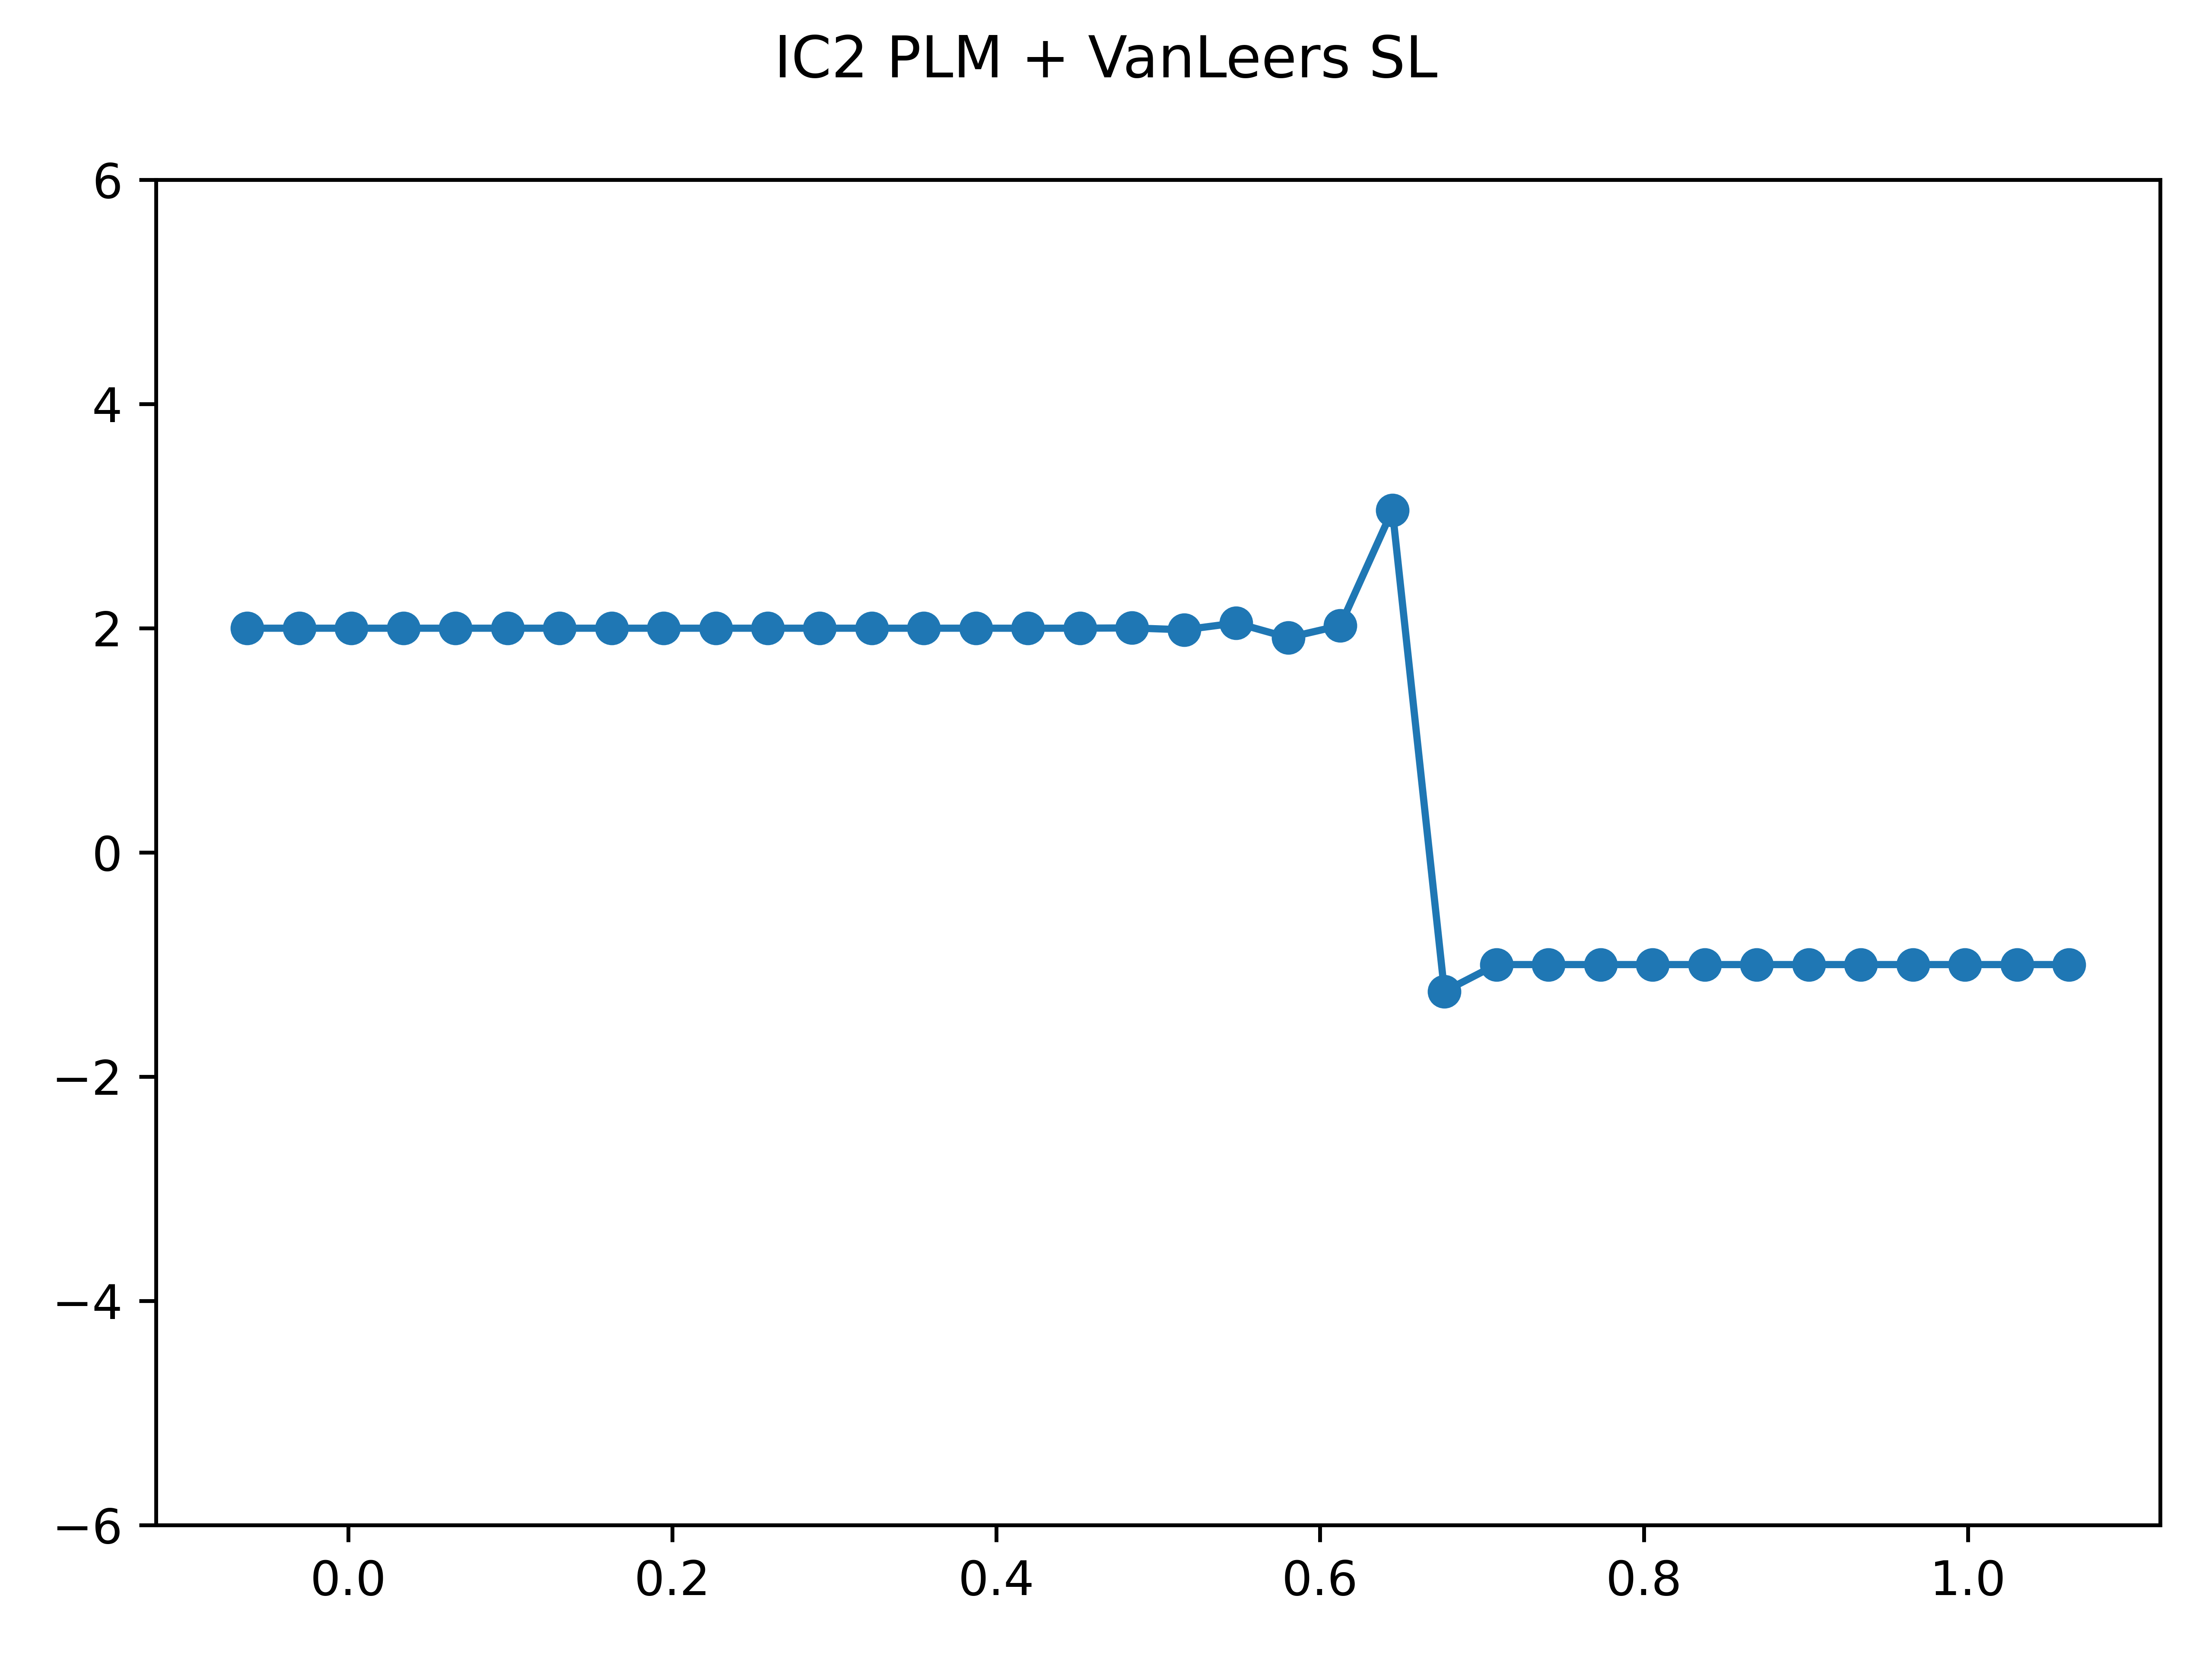
\includegraphics[width=.95\textwidth]{../../code/IC2Methodpv_plot.png}
        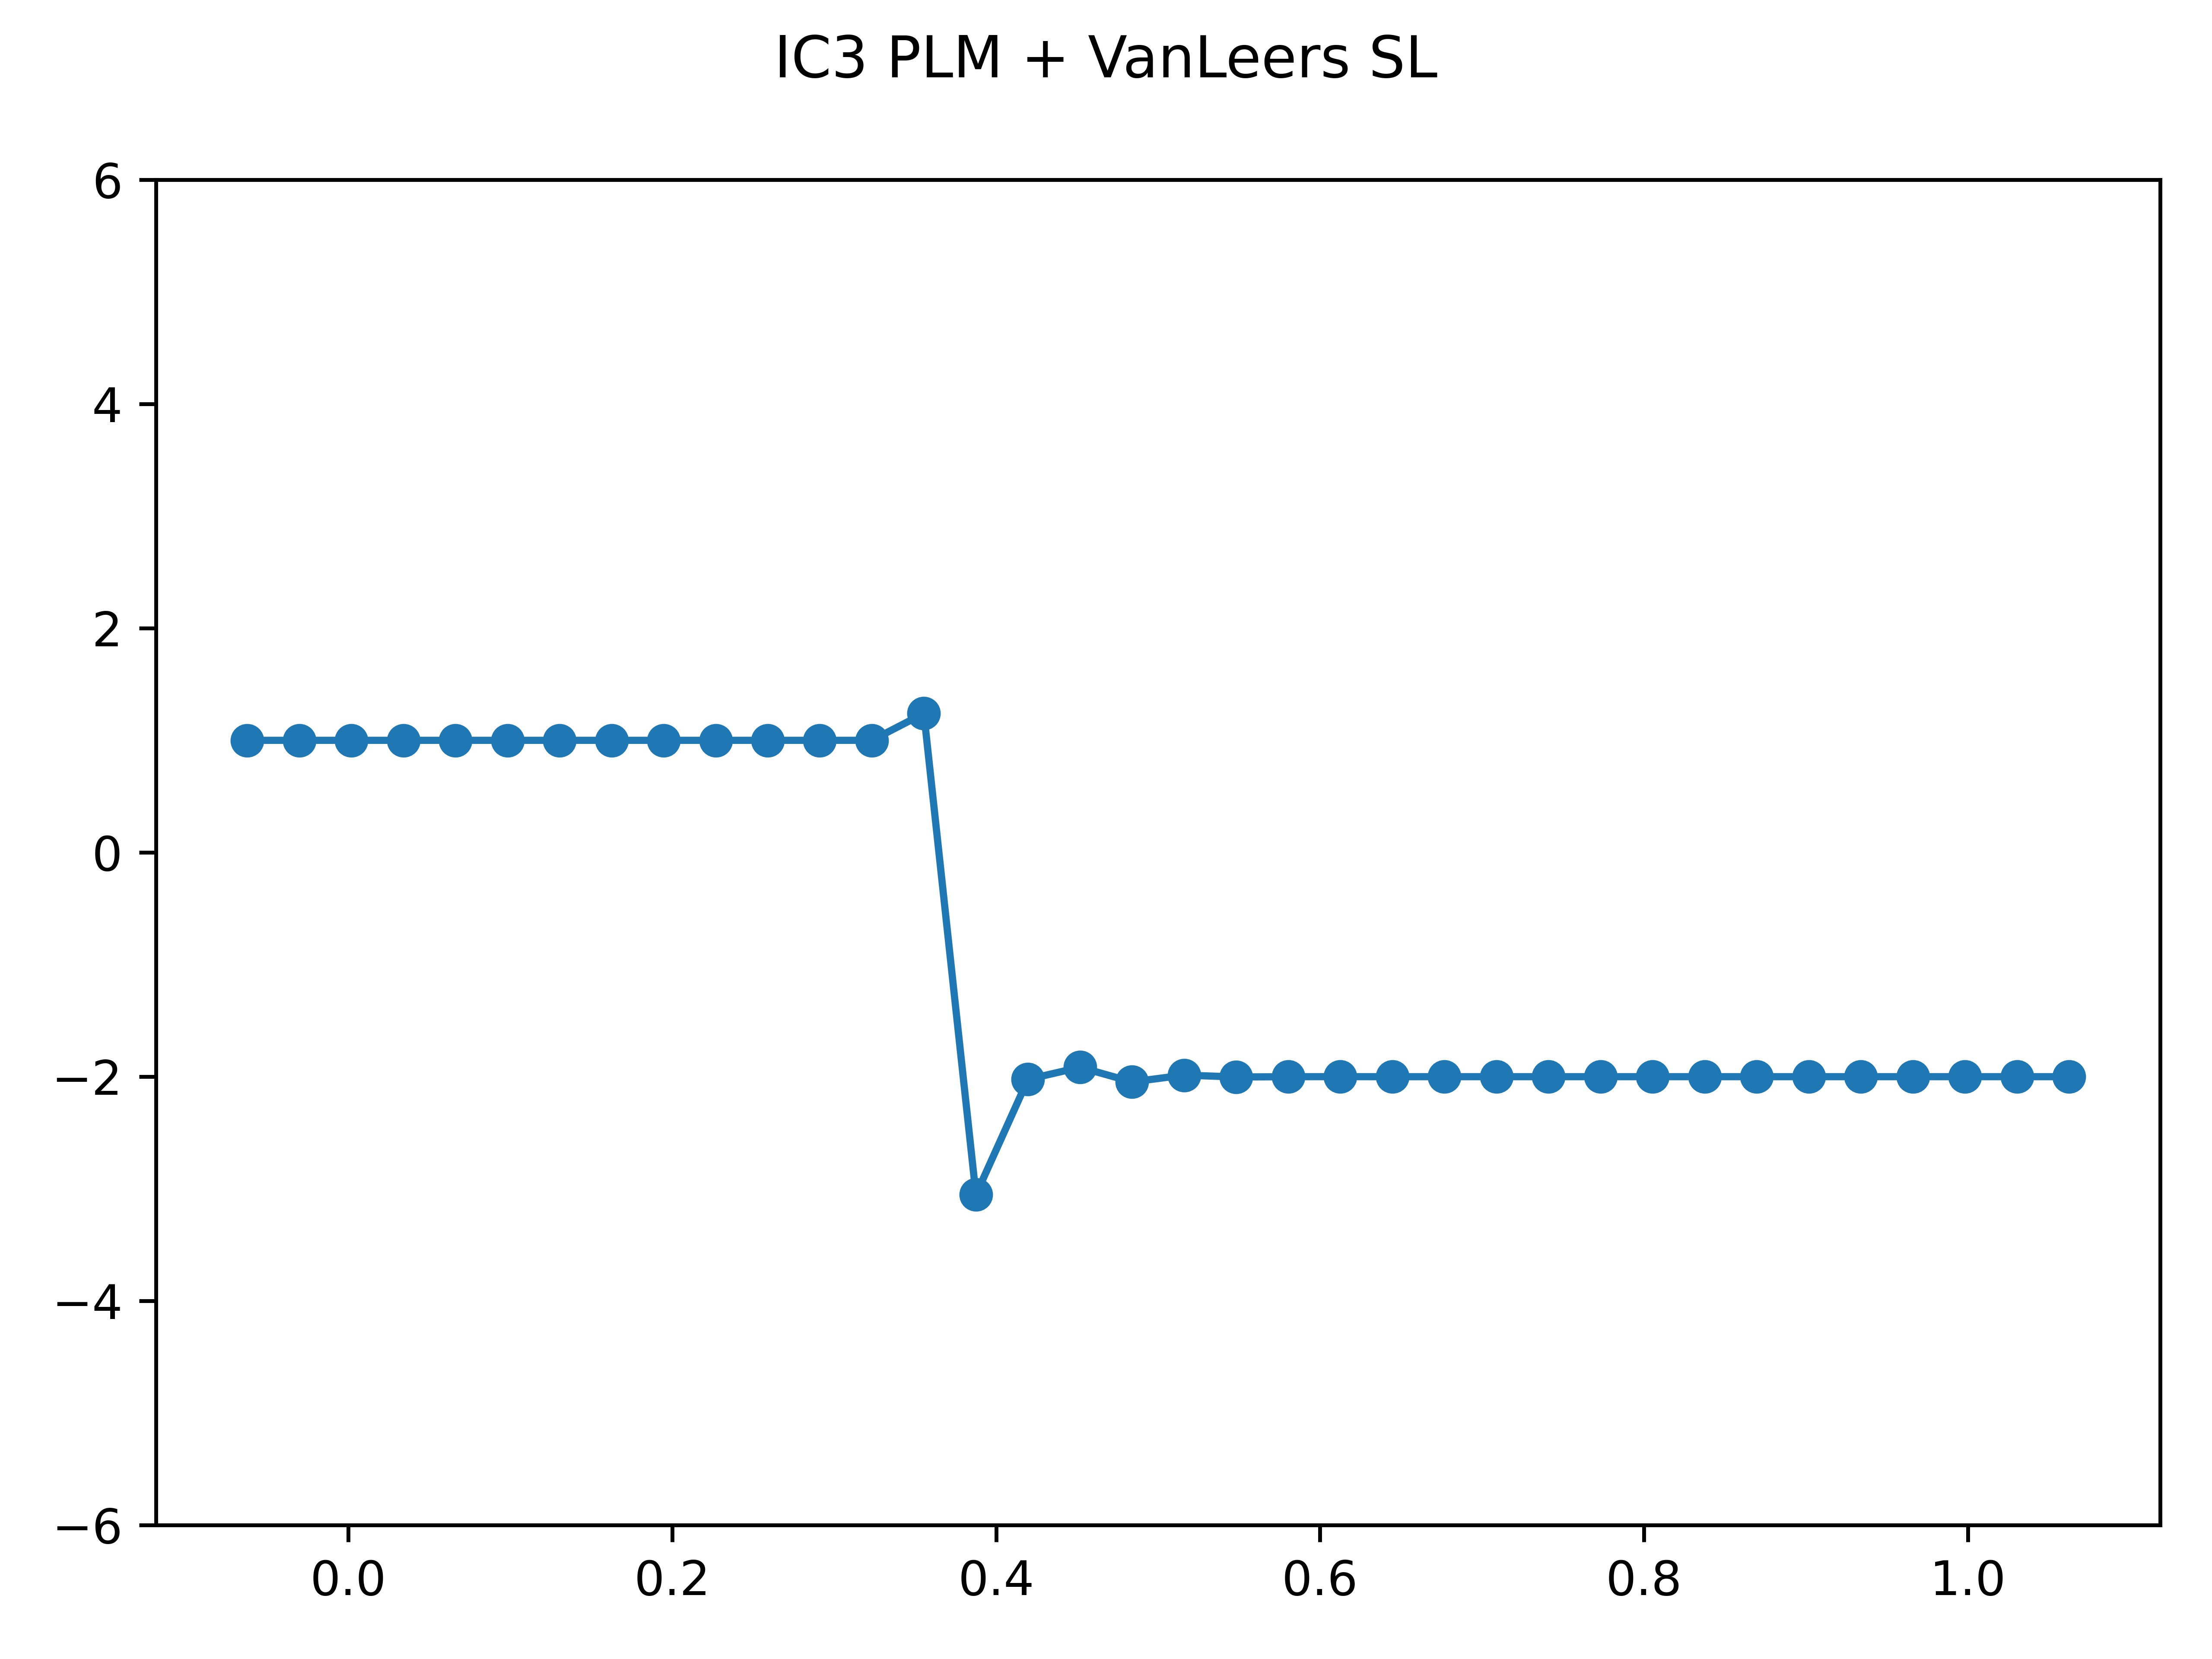
\includegraphics[width=.95\textwidth]{../../code/IC3Methodpv_plot.png}
        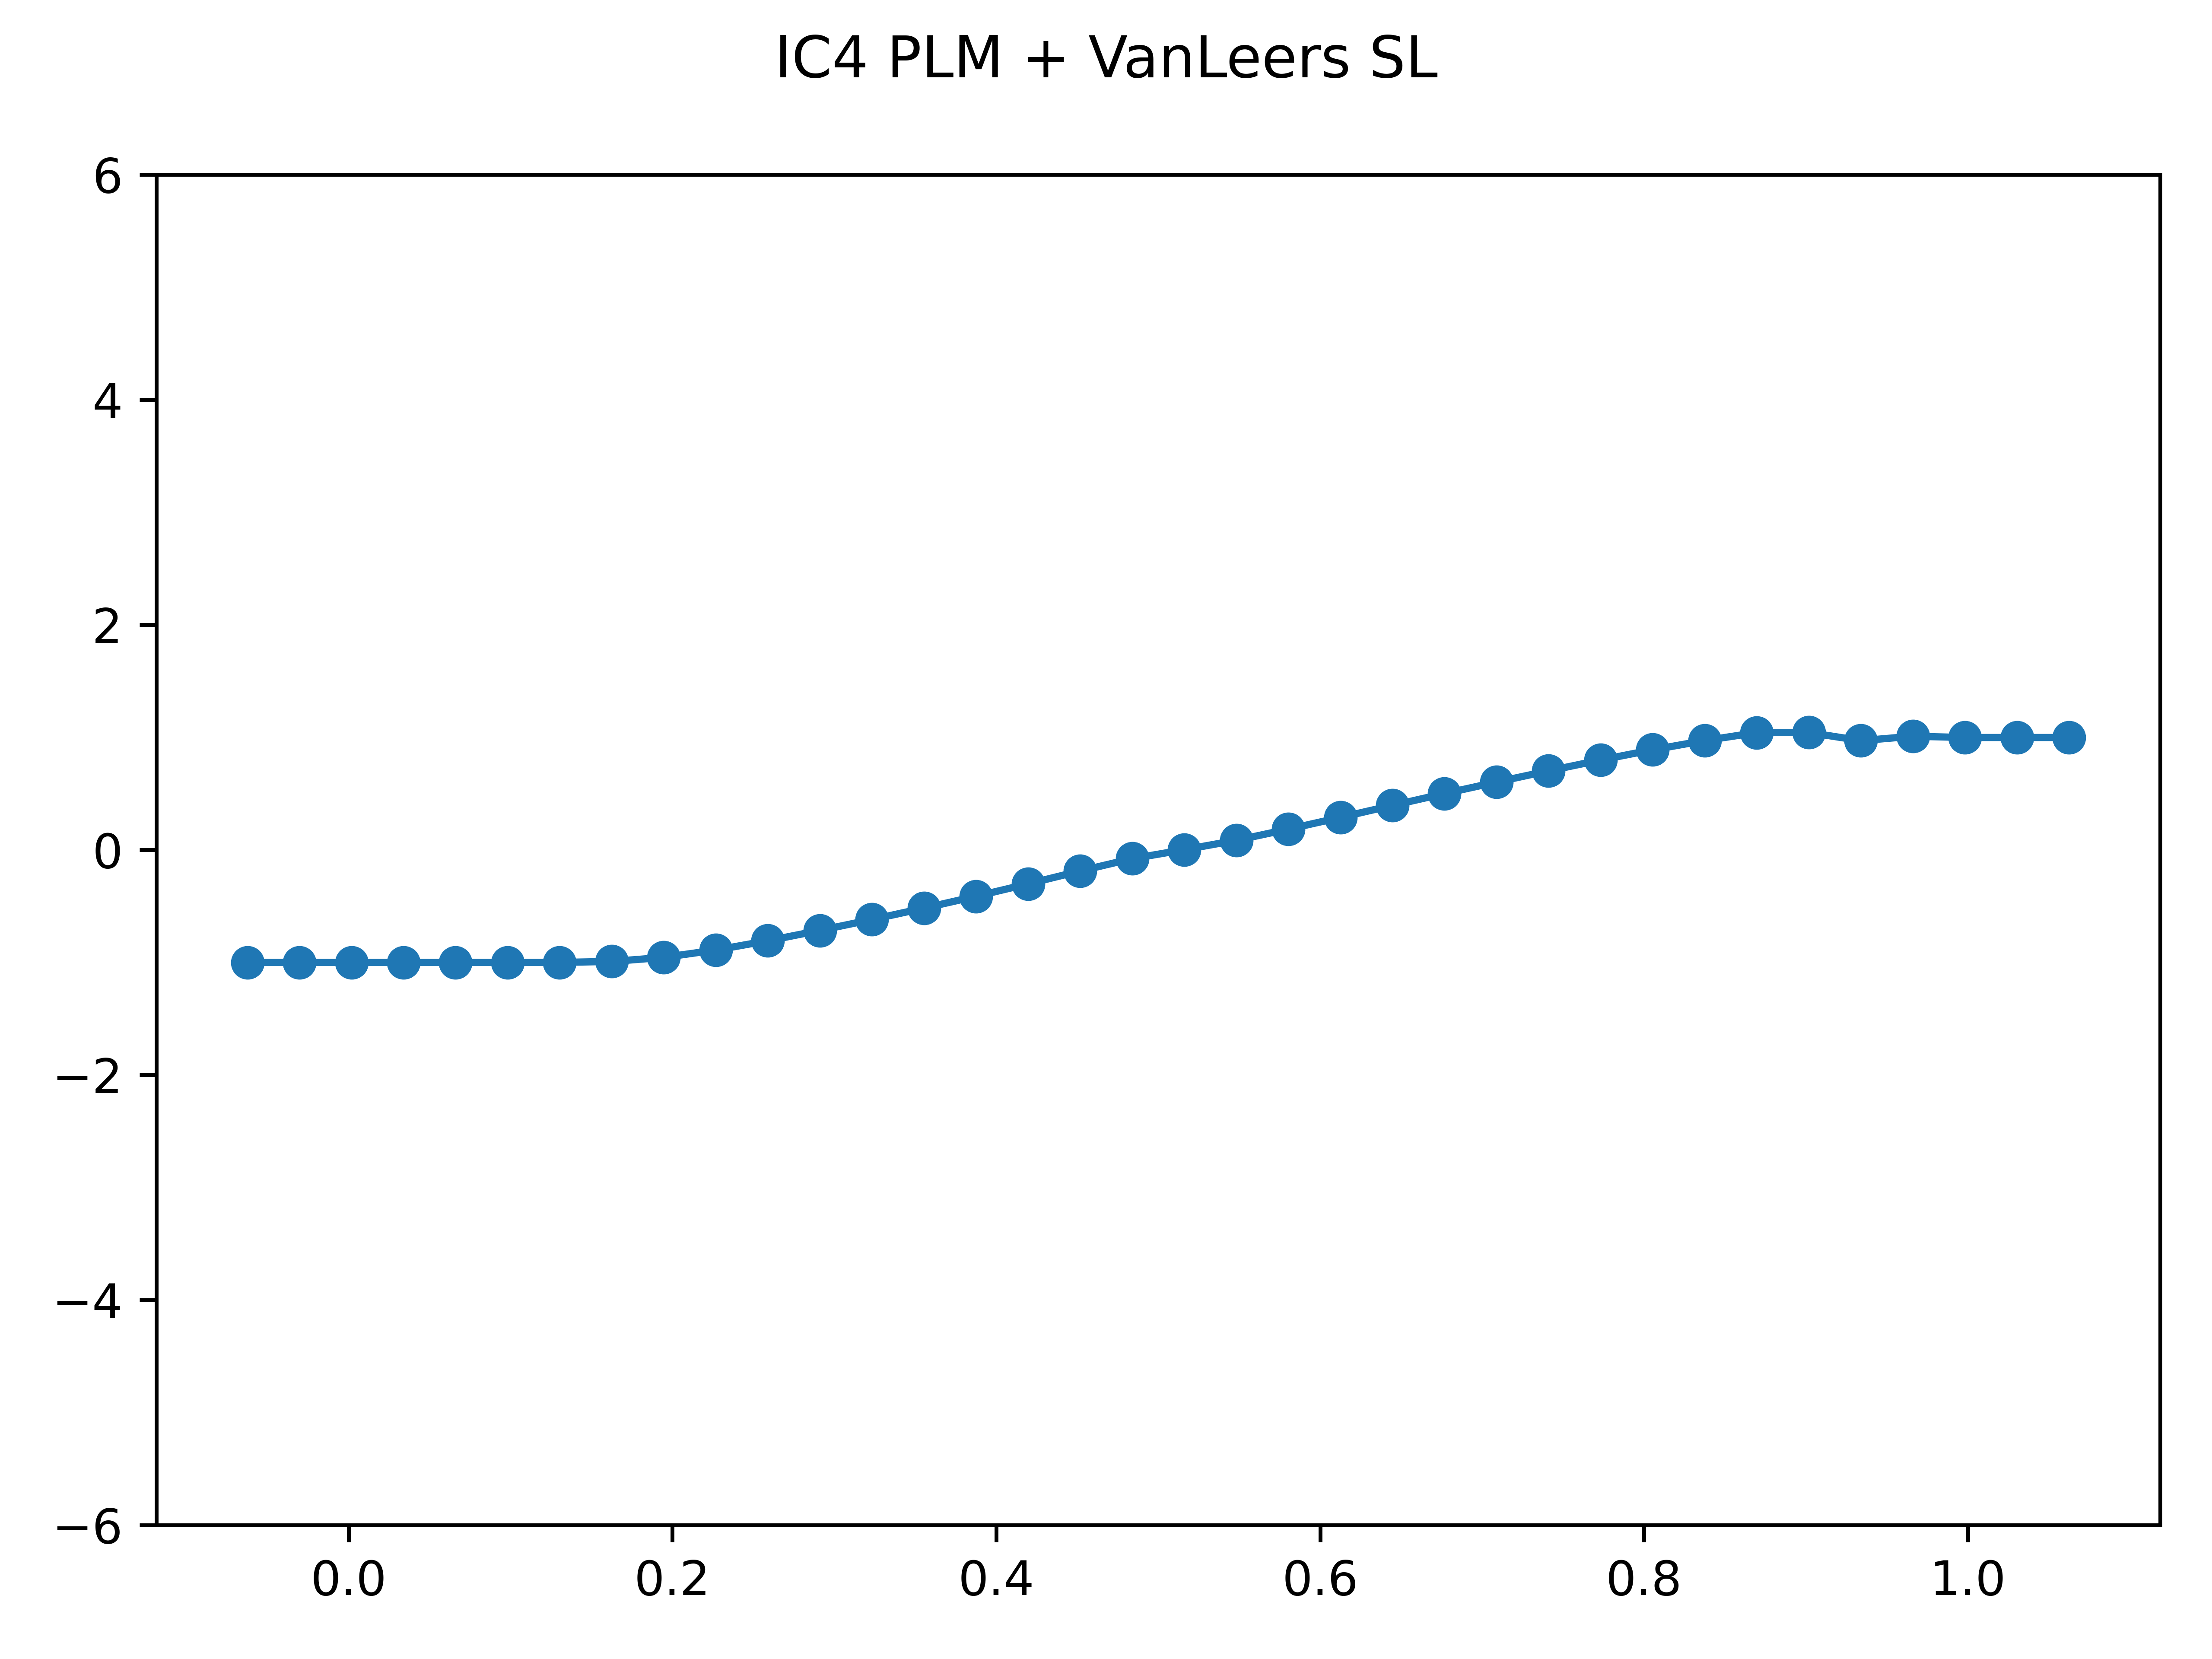
\includegraphics[width=.95\textwidth]{../../code/IC4Methodpv_plot.png}
        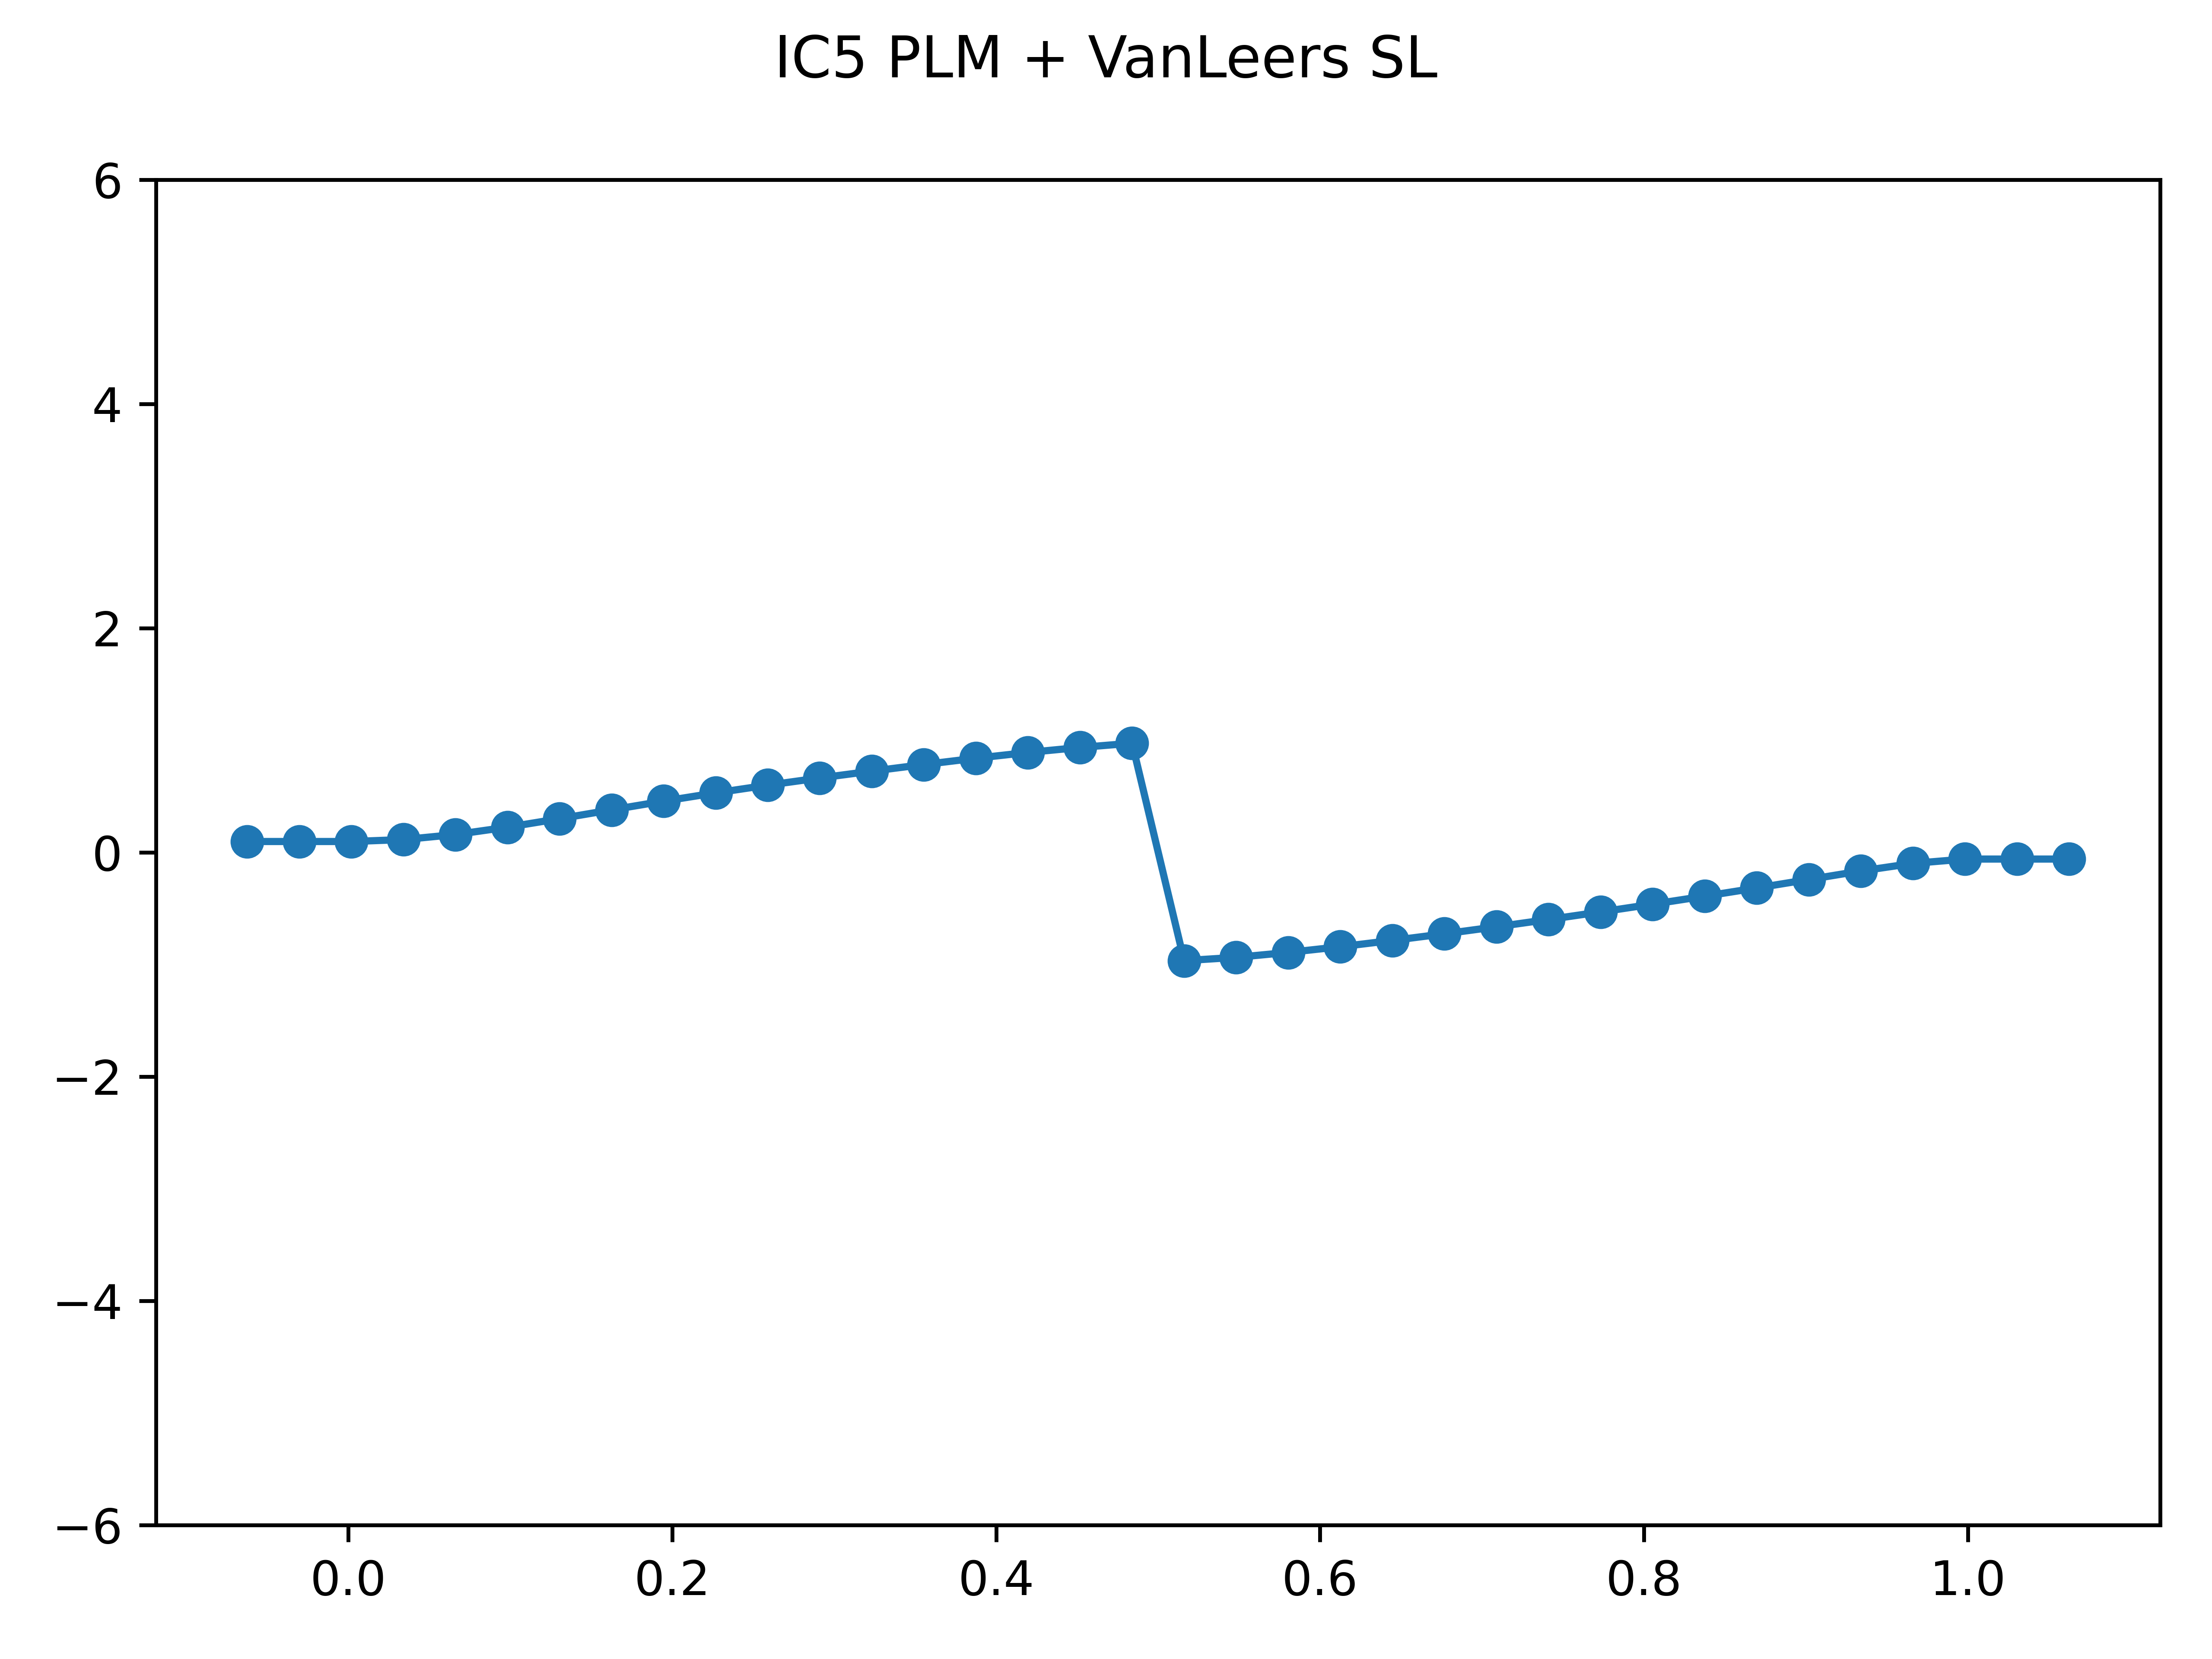
\includegraphics[width=.95\textwidth]{../../code/IC5Methodpv_plot.png}
        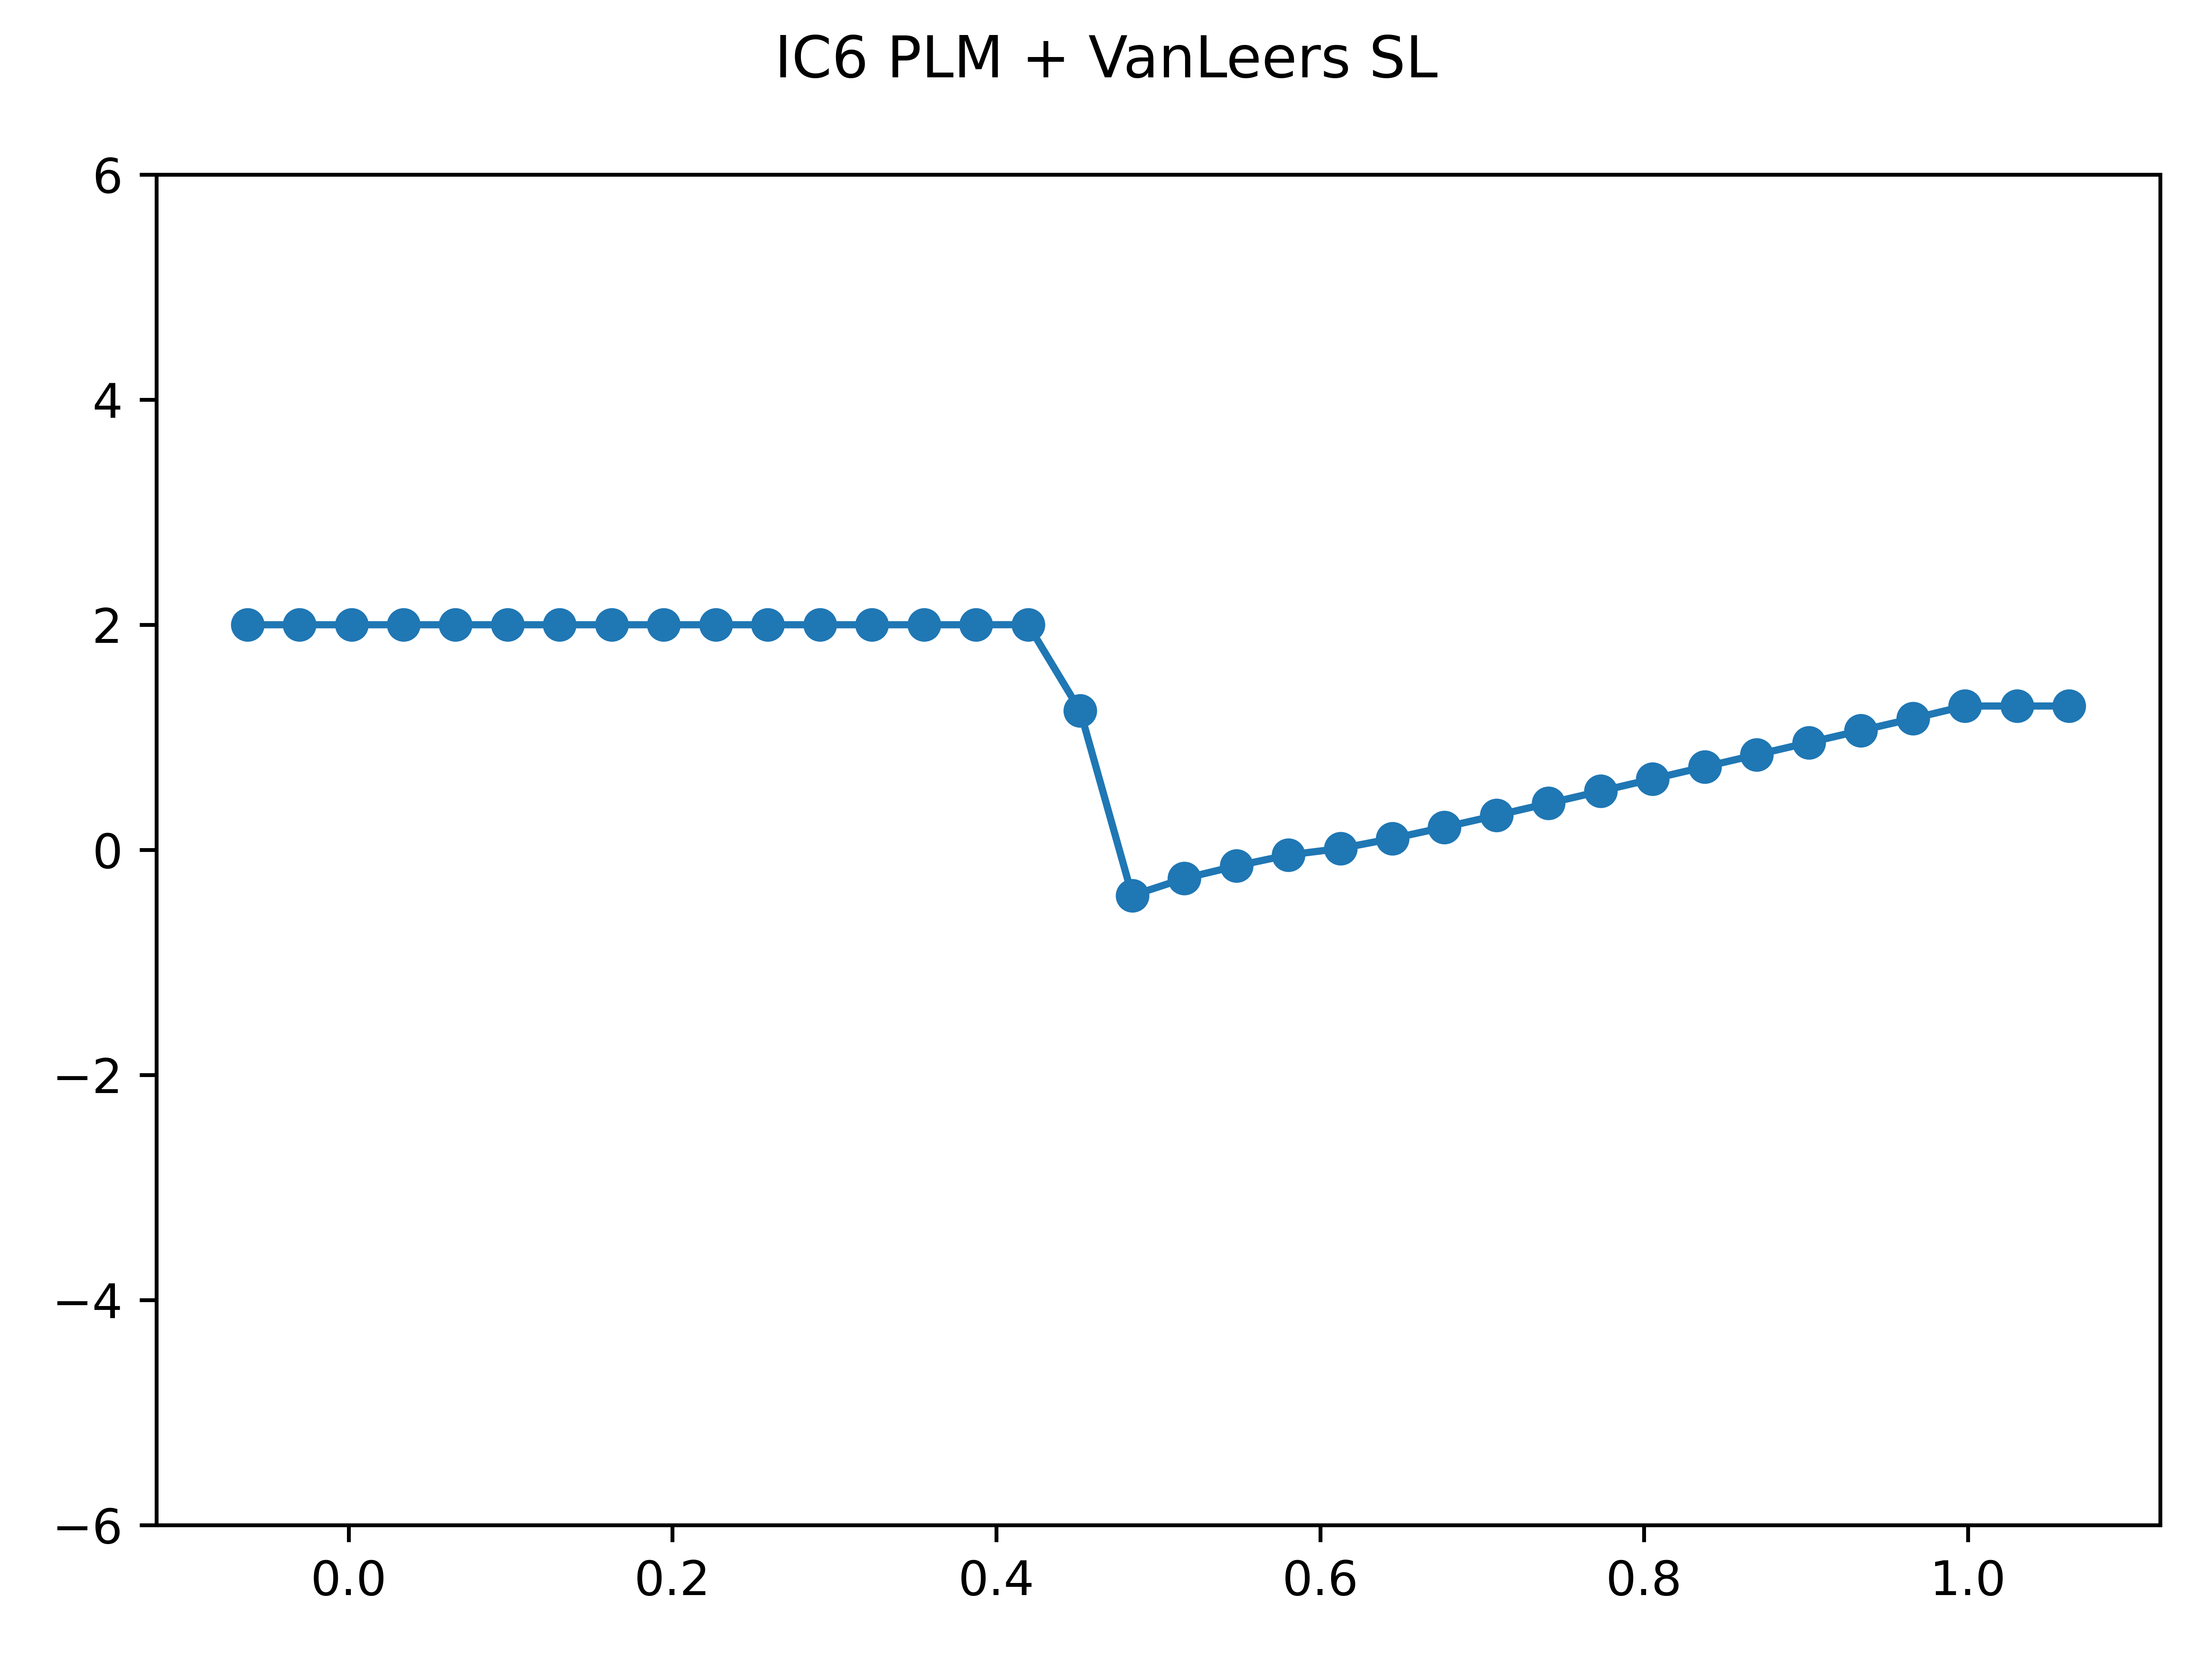
\includegraphics[width=.95\textwidth]{../../code/IC6Methodpv_plot.png}
    \emp
    \caption{Initial Conditions 1-6 (rows) at t=0.3 (or as close as possible before the
    solver crashed for each run). The columns are from left to right, the FOG,
    PLM + Minmod, PLM + MC, and PLM + VanLeers solvers.}
    \label{fig:sol_1_6}
\end{figure}

\begin{figure}[t]
    \bmp{0.25}
        \centering
        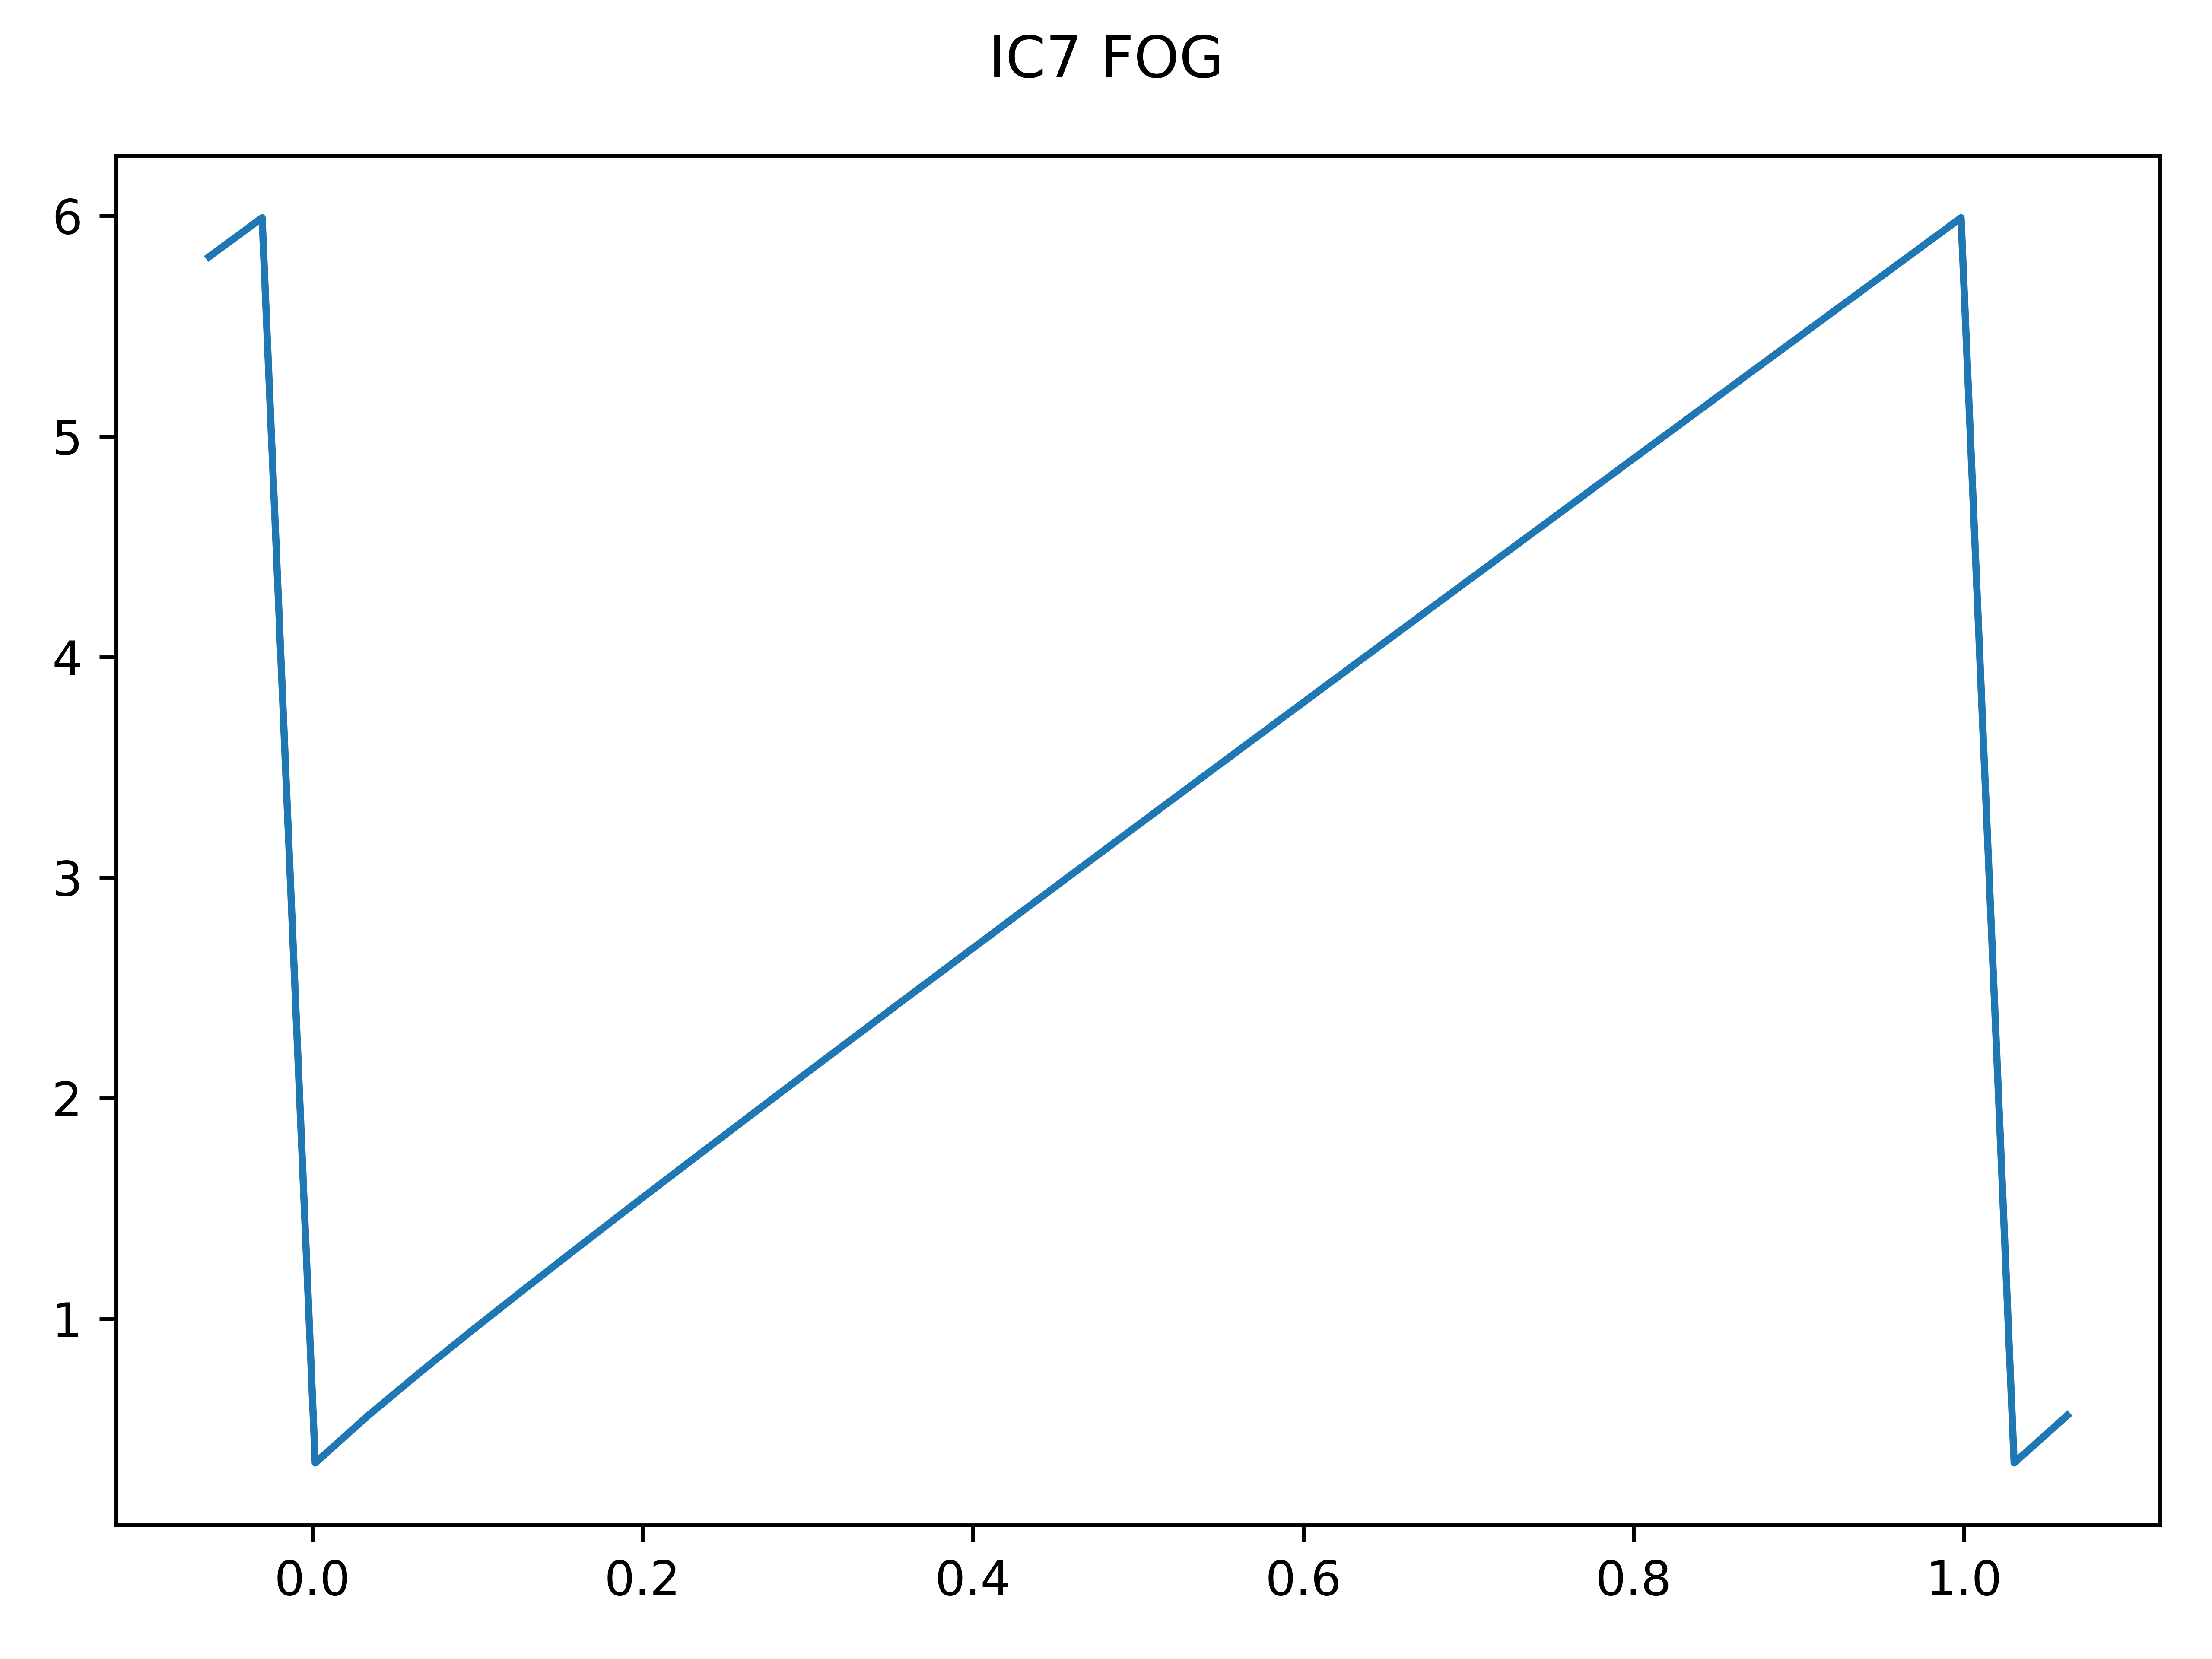
\includegraphics[width=.95\textwidth]{../../code/IC7Methodfu_plot.png}
        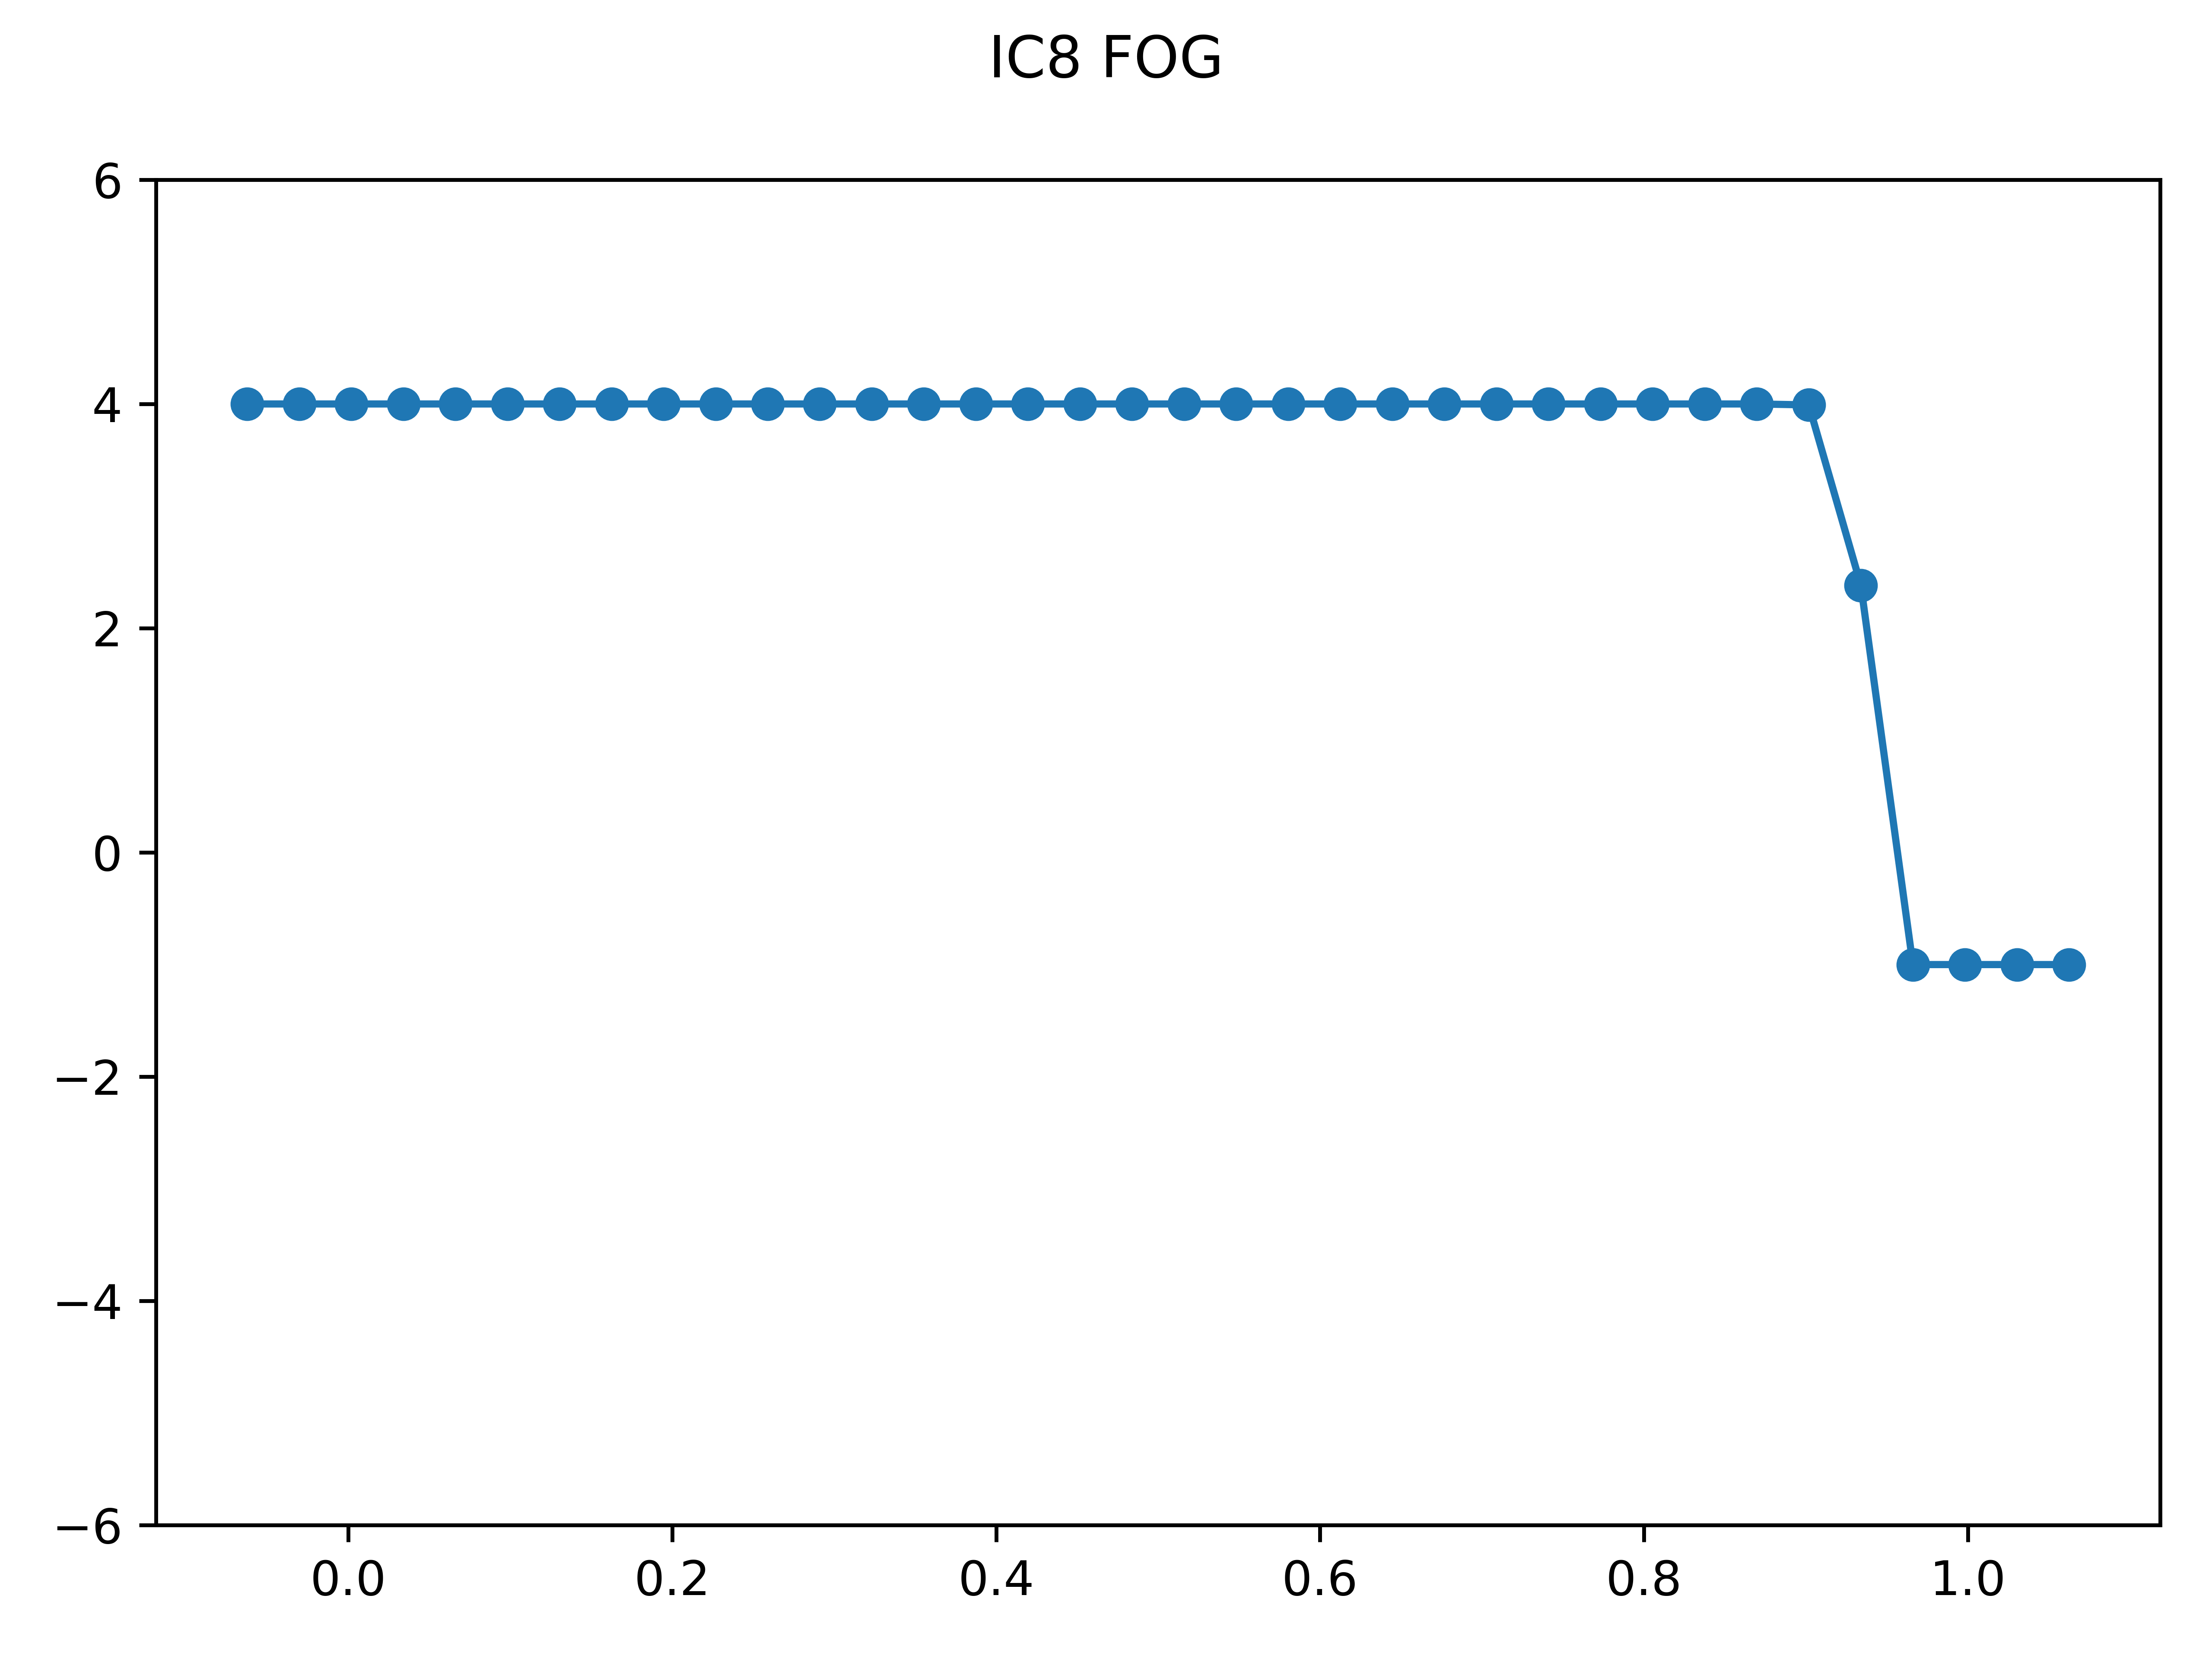
\includegraphics[width=.95\textwidth]{../../code/IC8Methodfu_plot.png}
        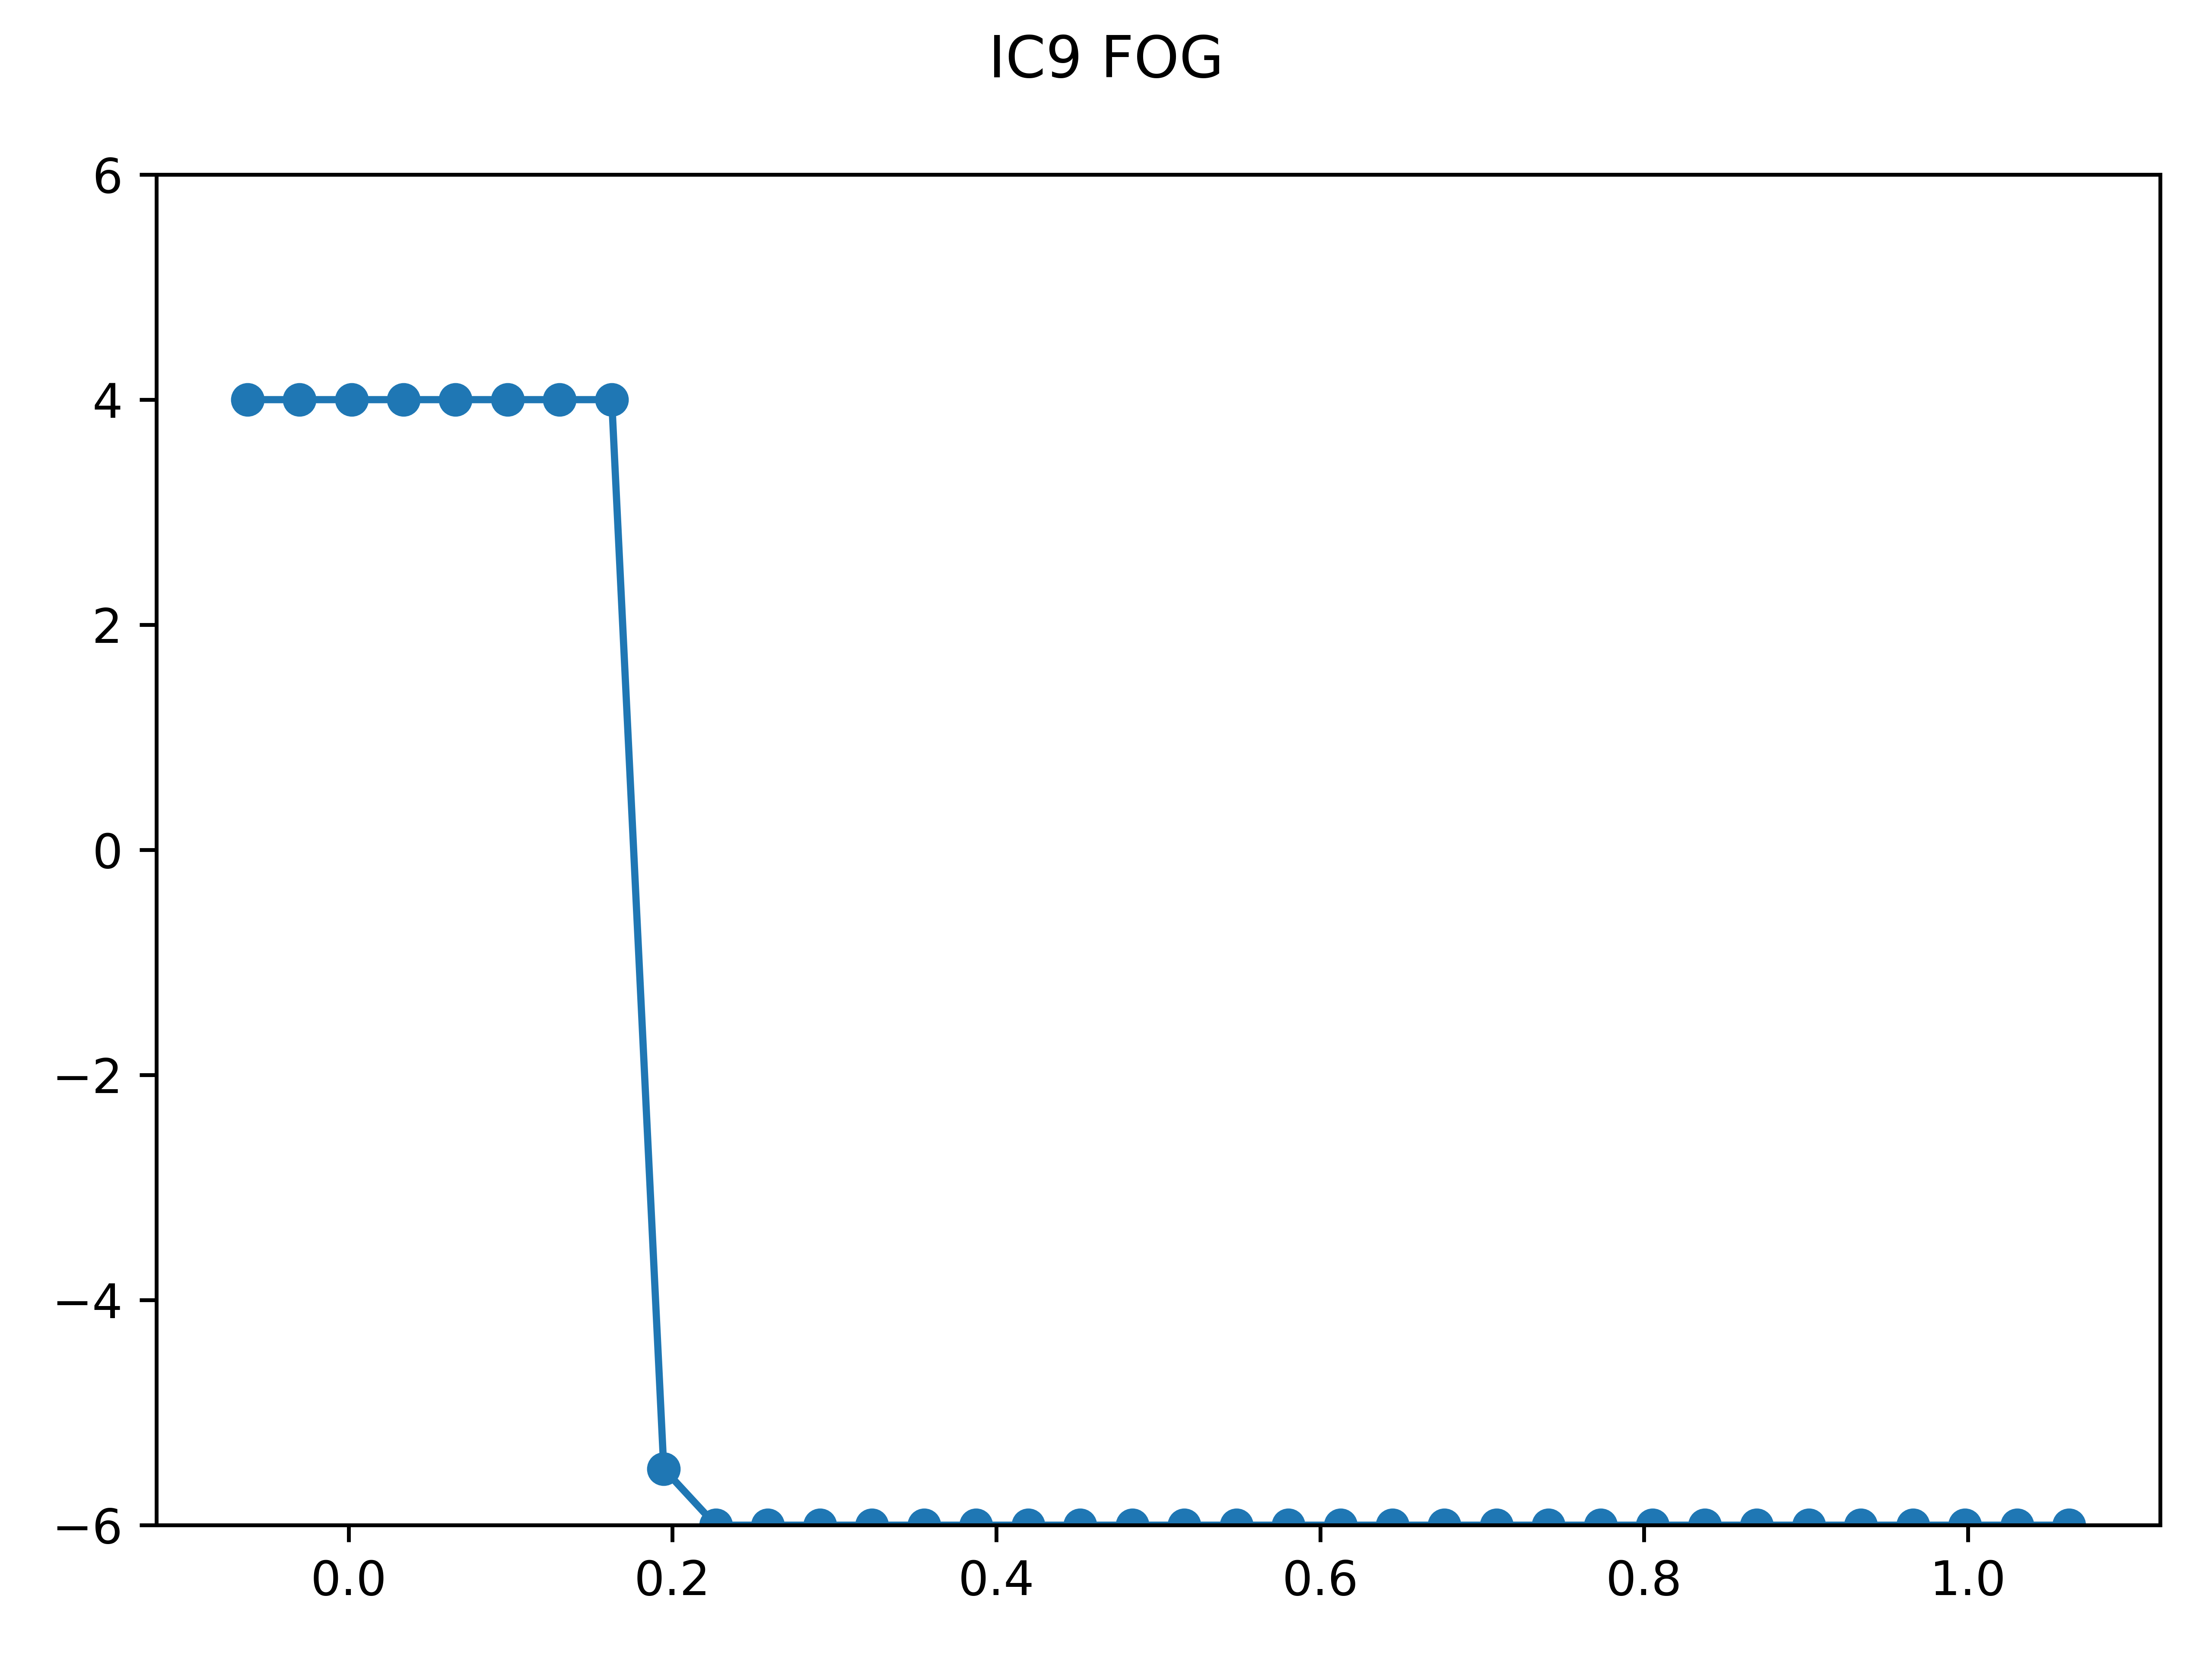
\includegraphics[width=.95\textwidth]{../../code/IC9Methodfu_plot.png}
        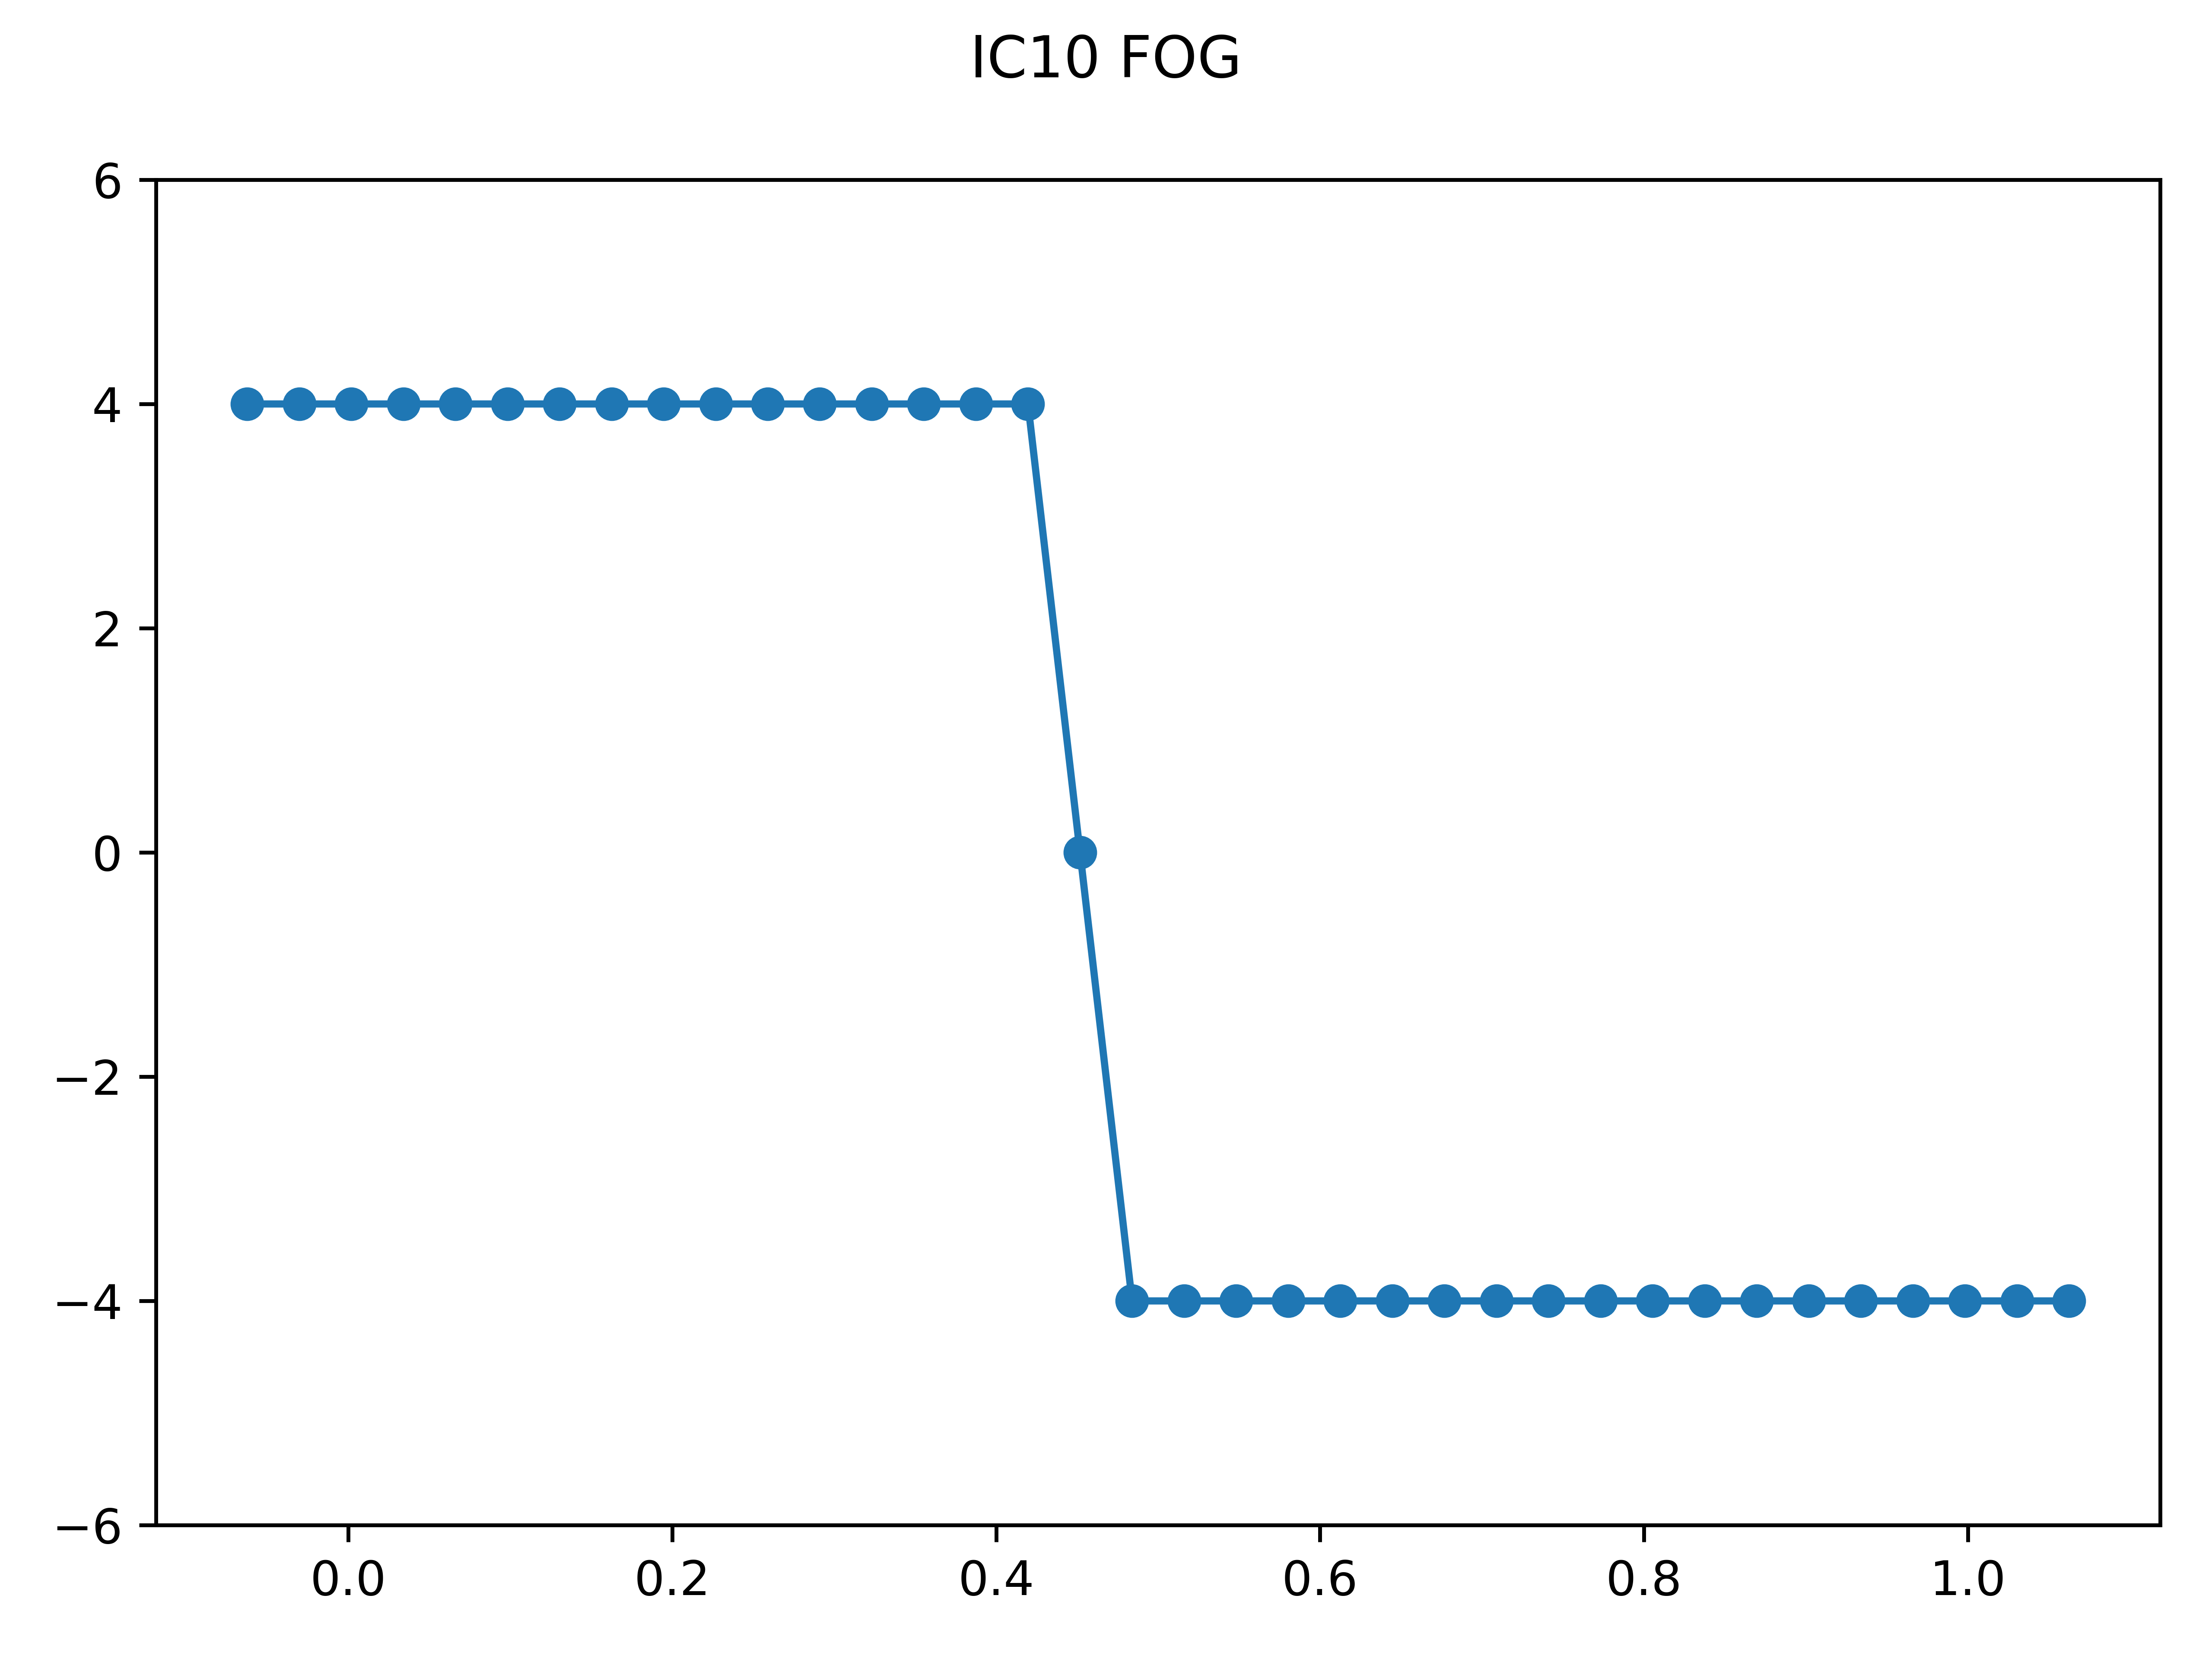
\includegraphics[width=.95\textwidth]{../../code/IC10Methodfu_plot.png}
        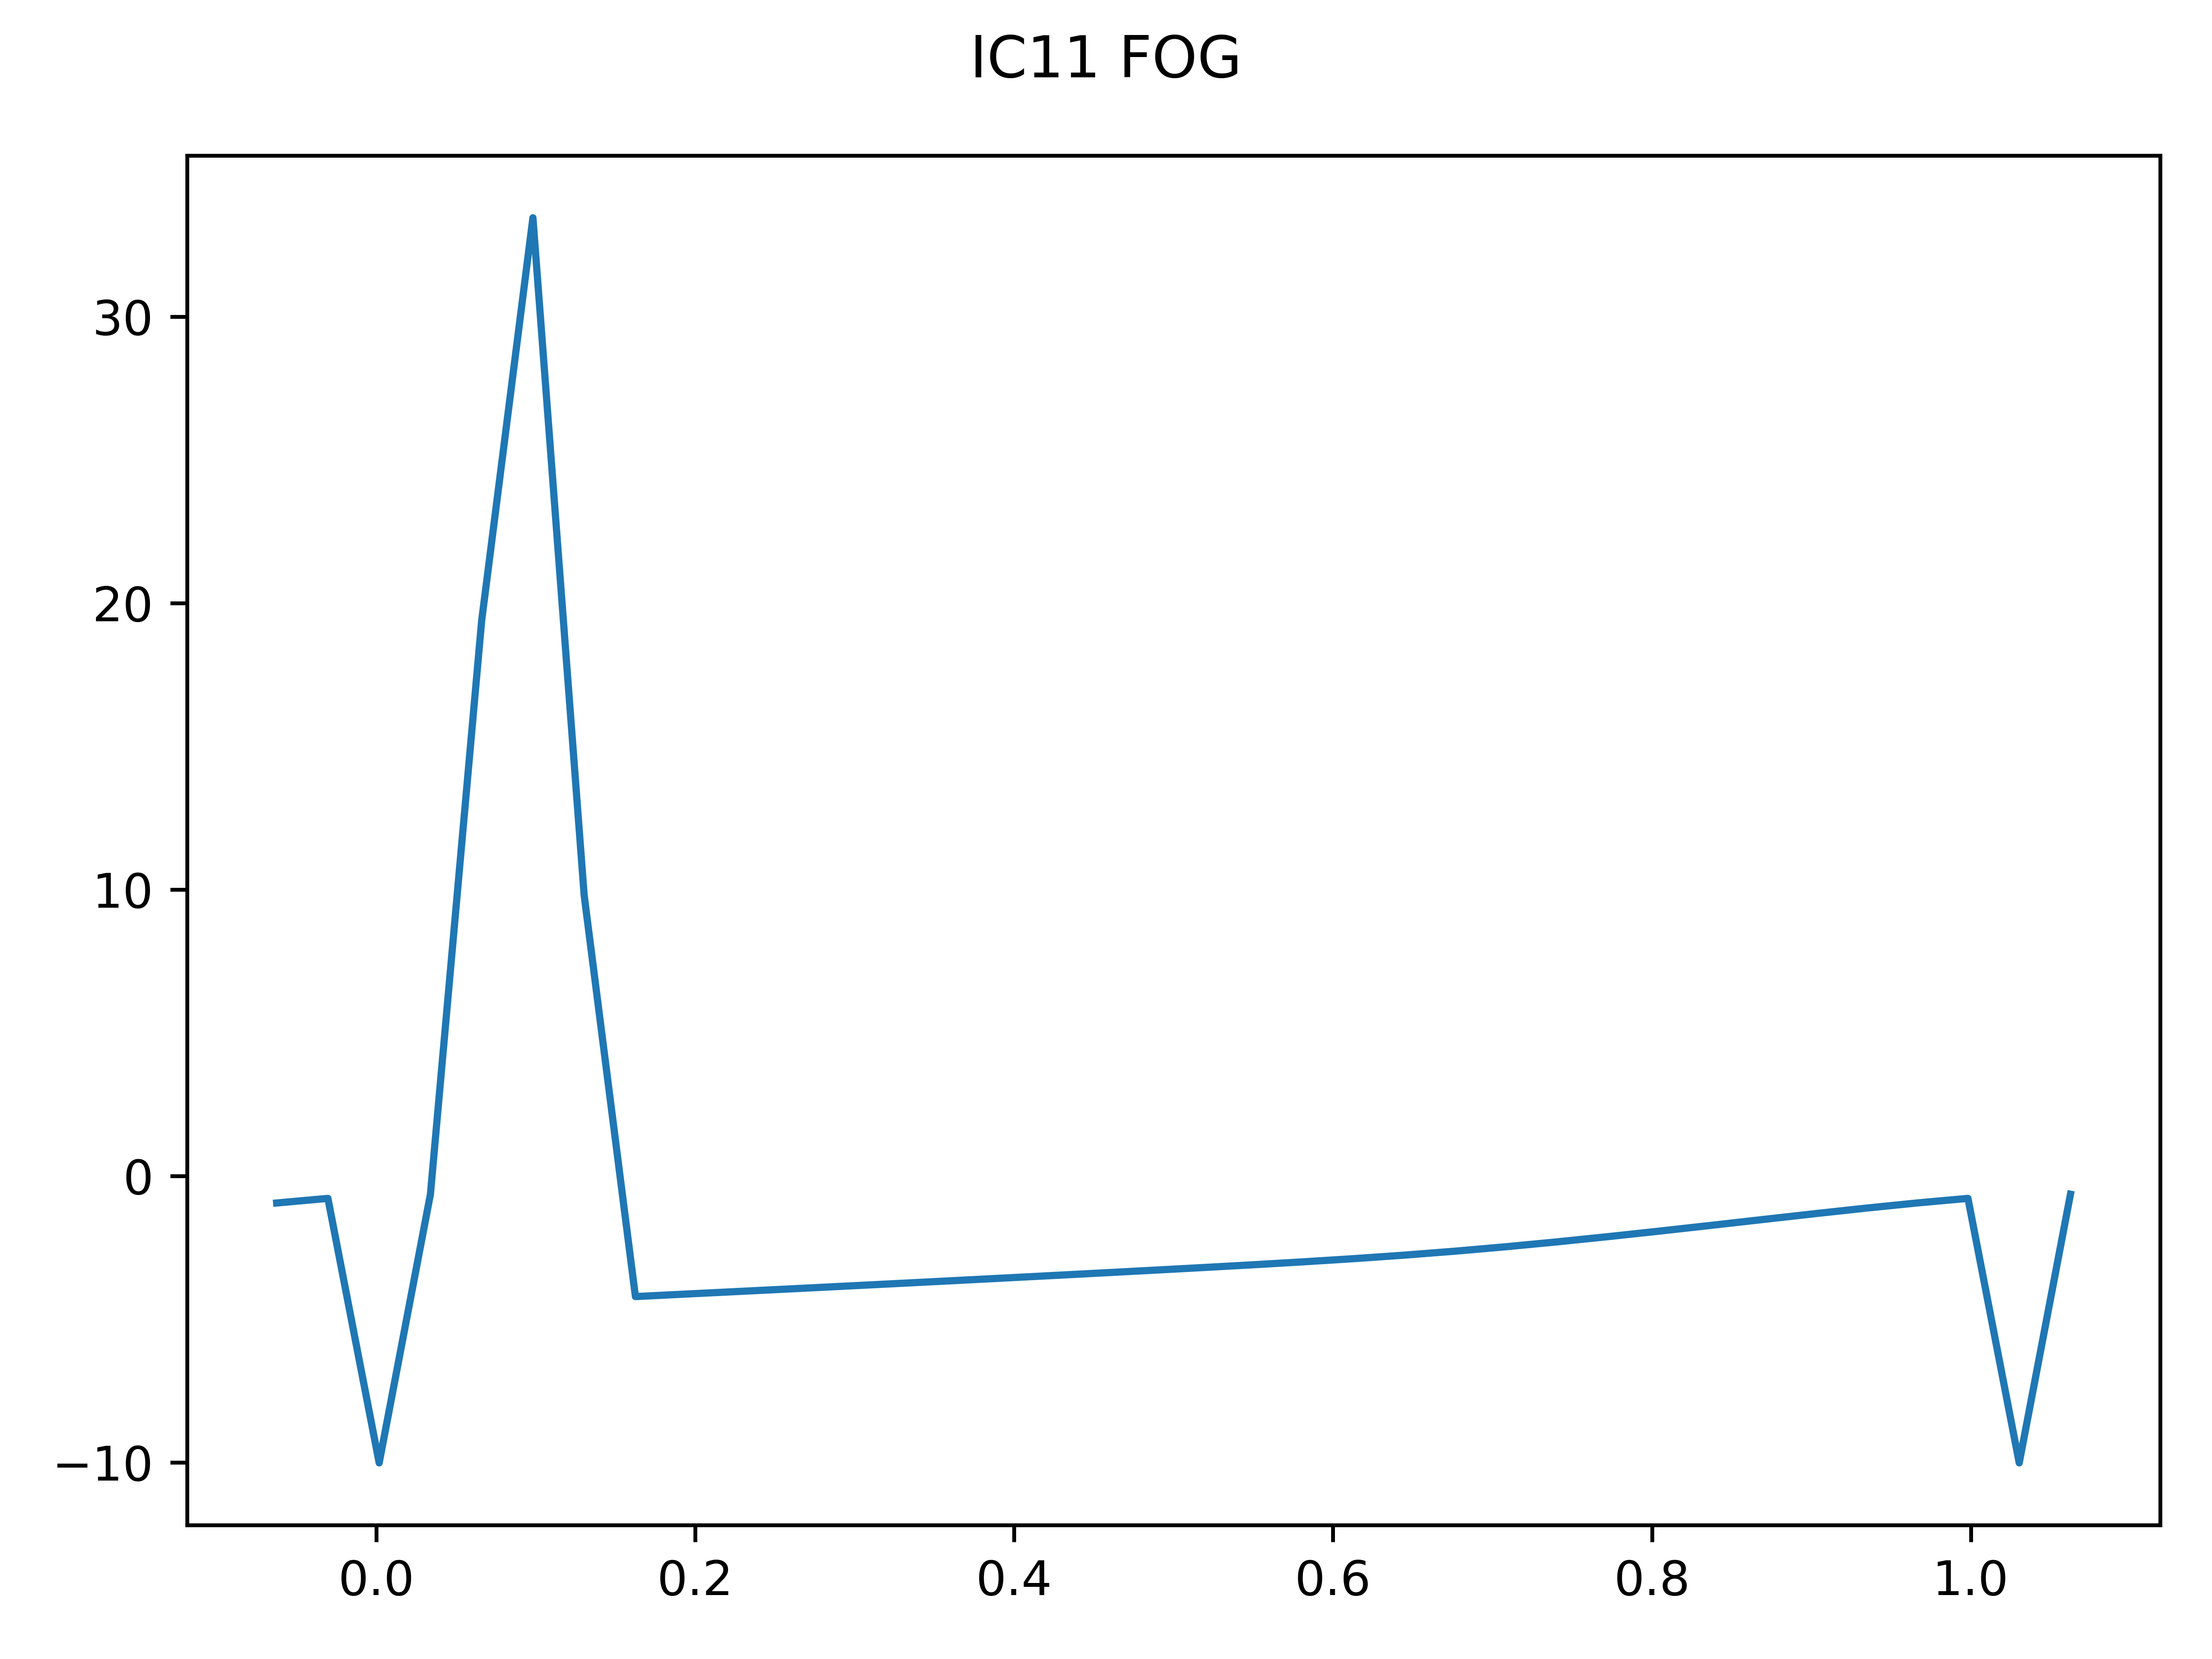
\includegraphics[width=.95\textwidth]{../../code/IC11Methodfu_plot.png}
    \emp
    \bmp{0.25}
        \centering
        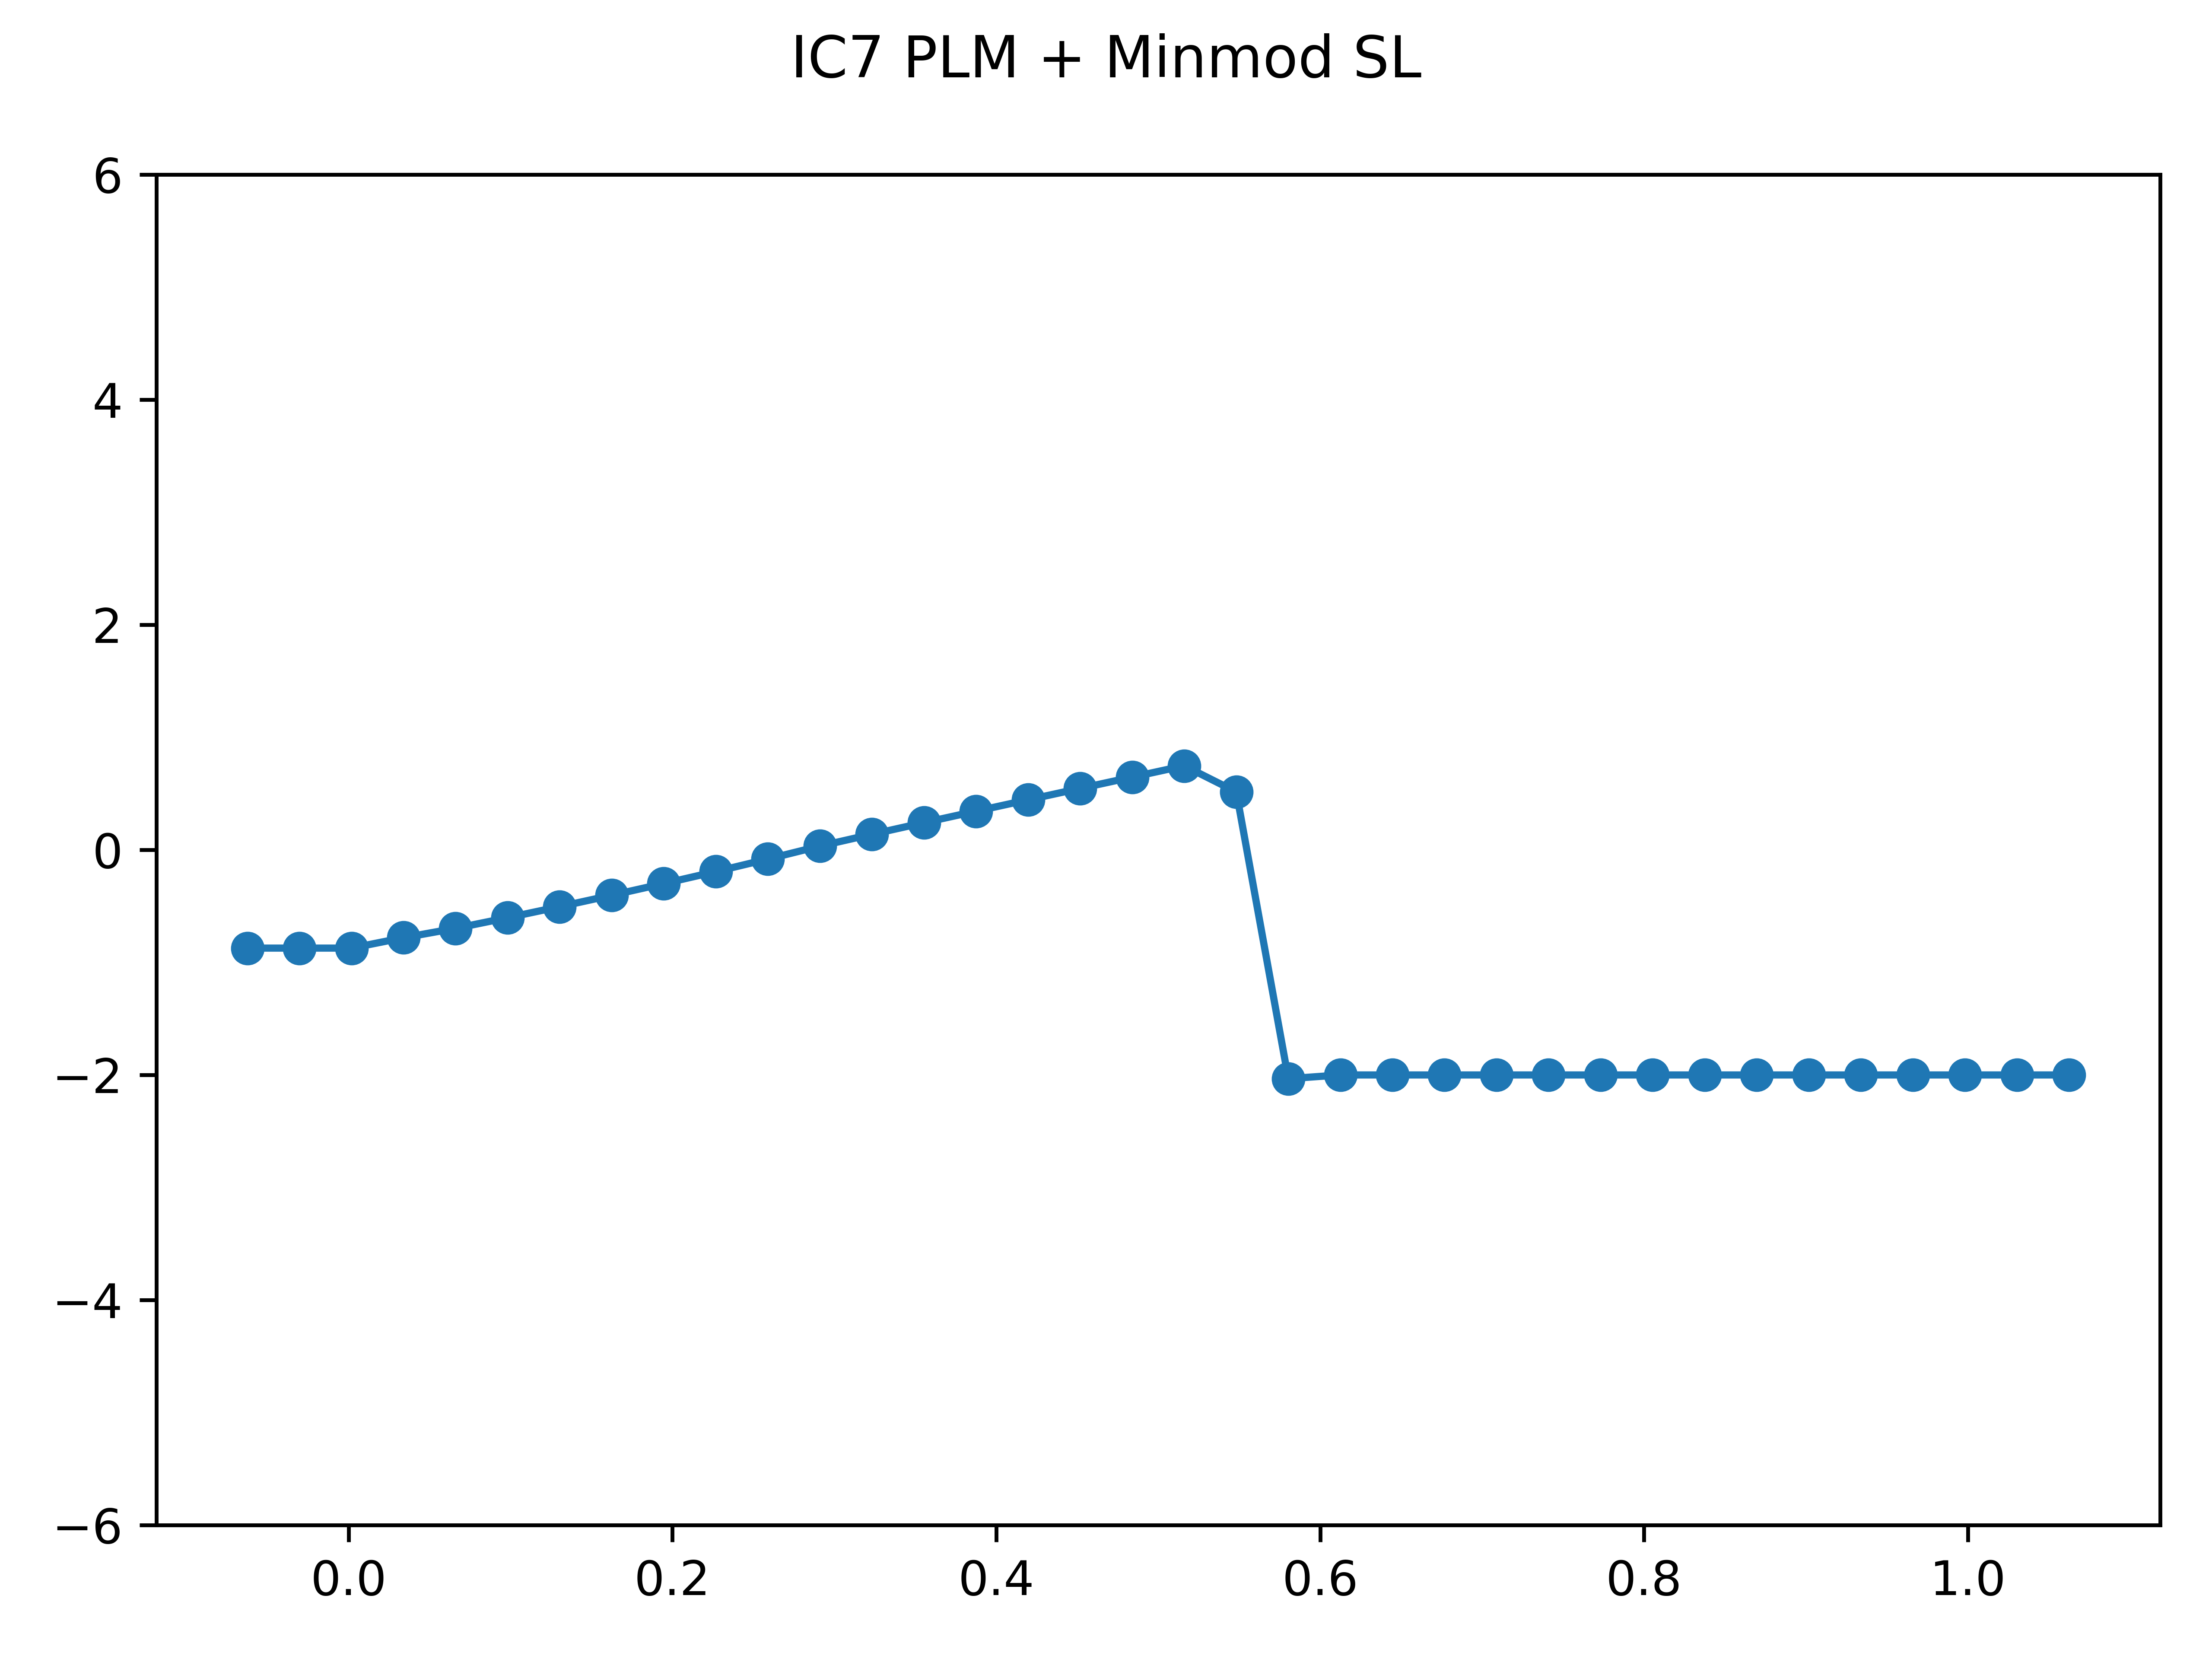
\includegraphics[width=.95\textwidth]{../../code/IC7Methodpm_plot.png}
        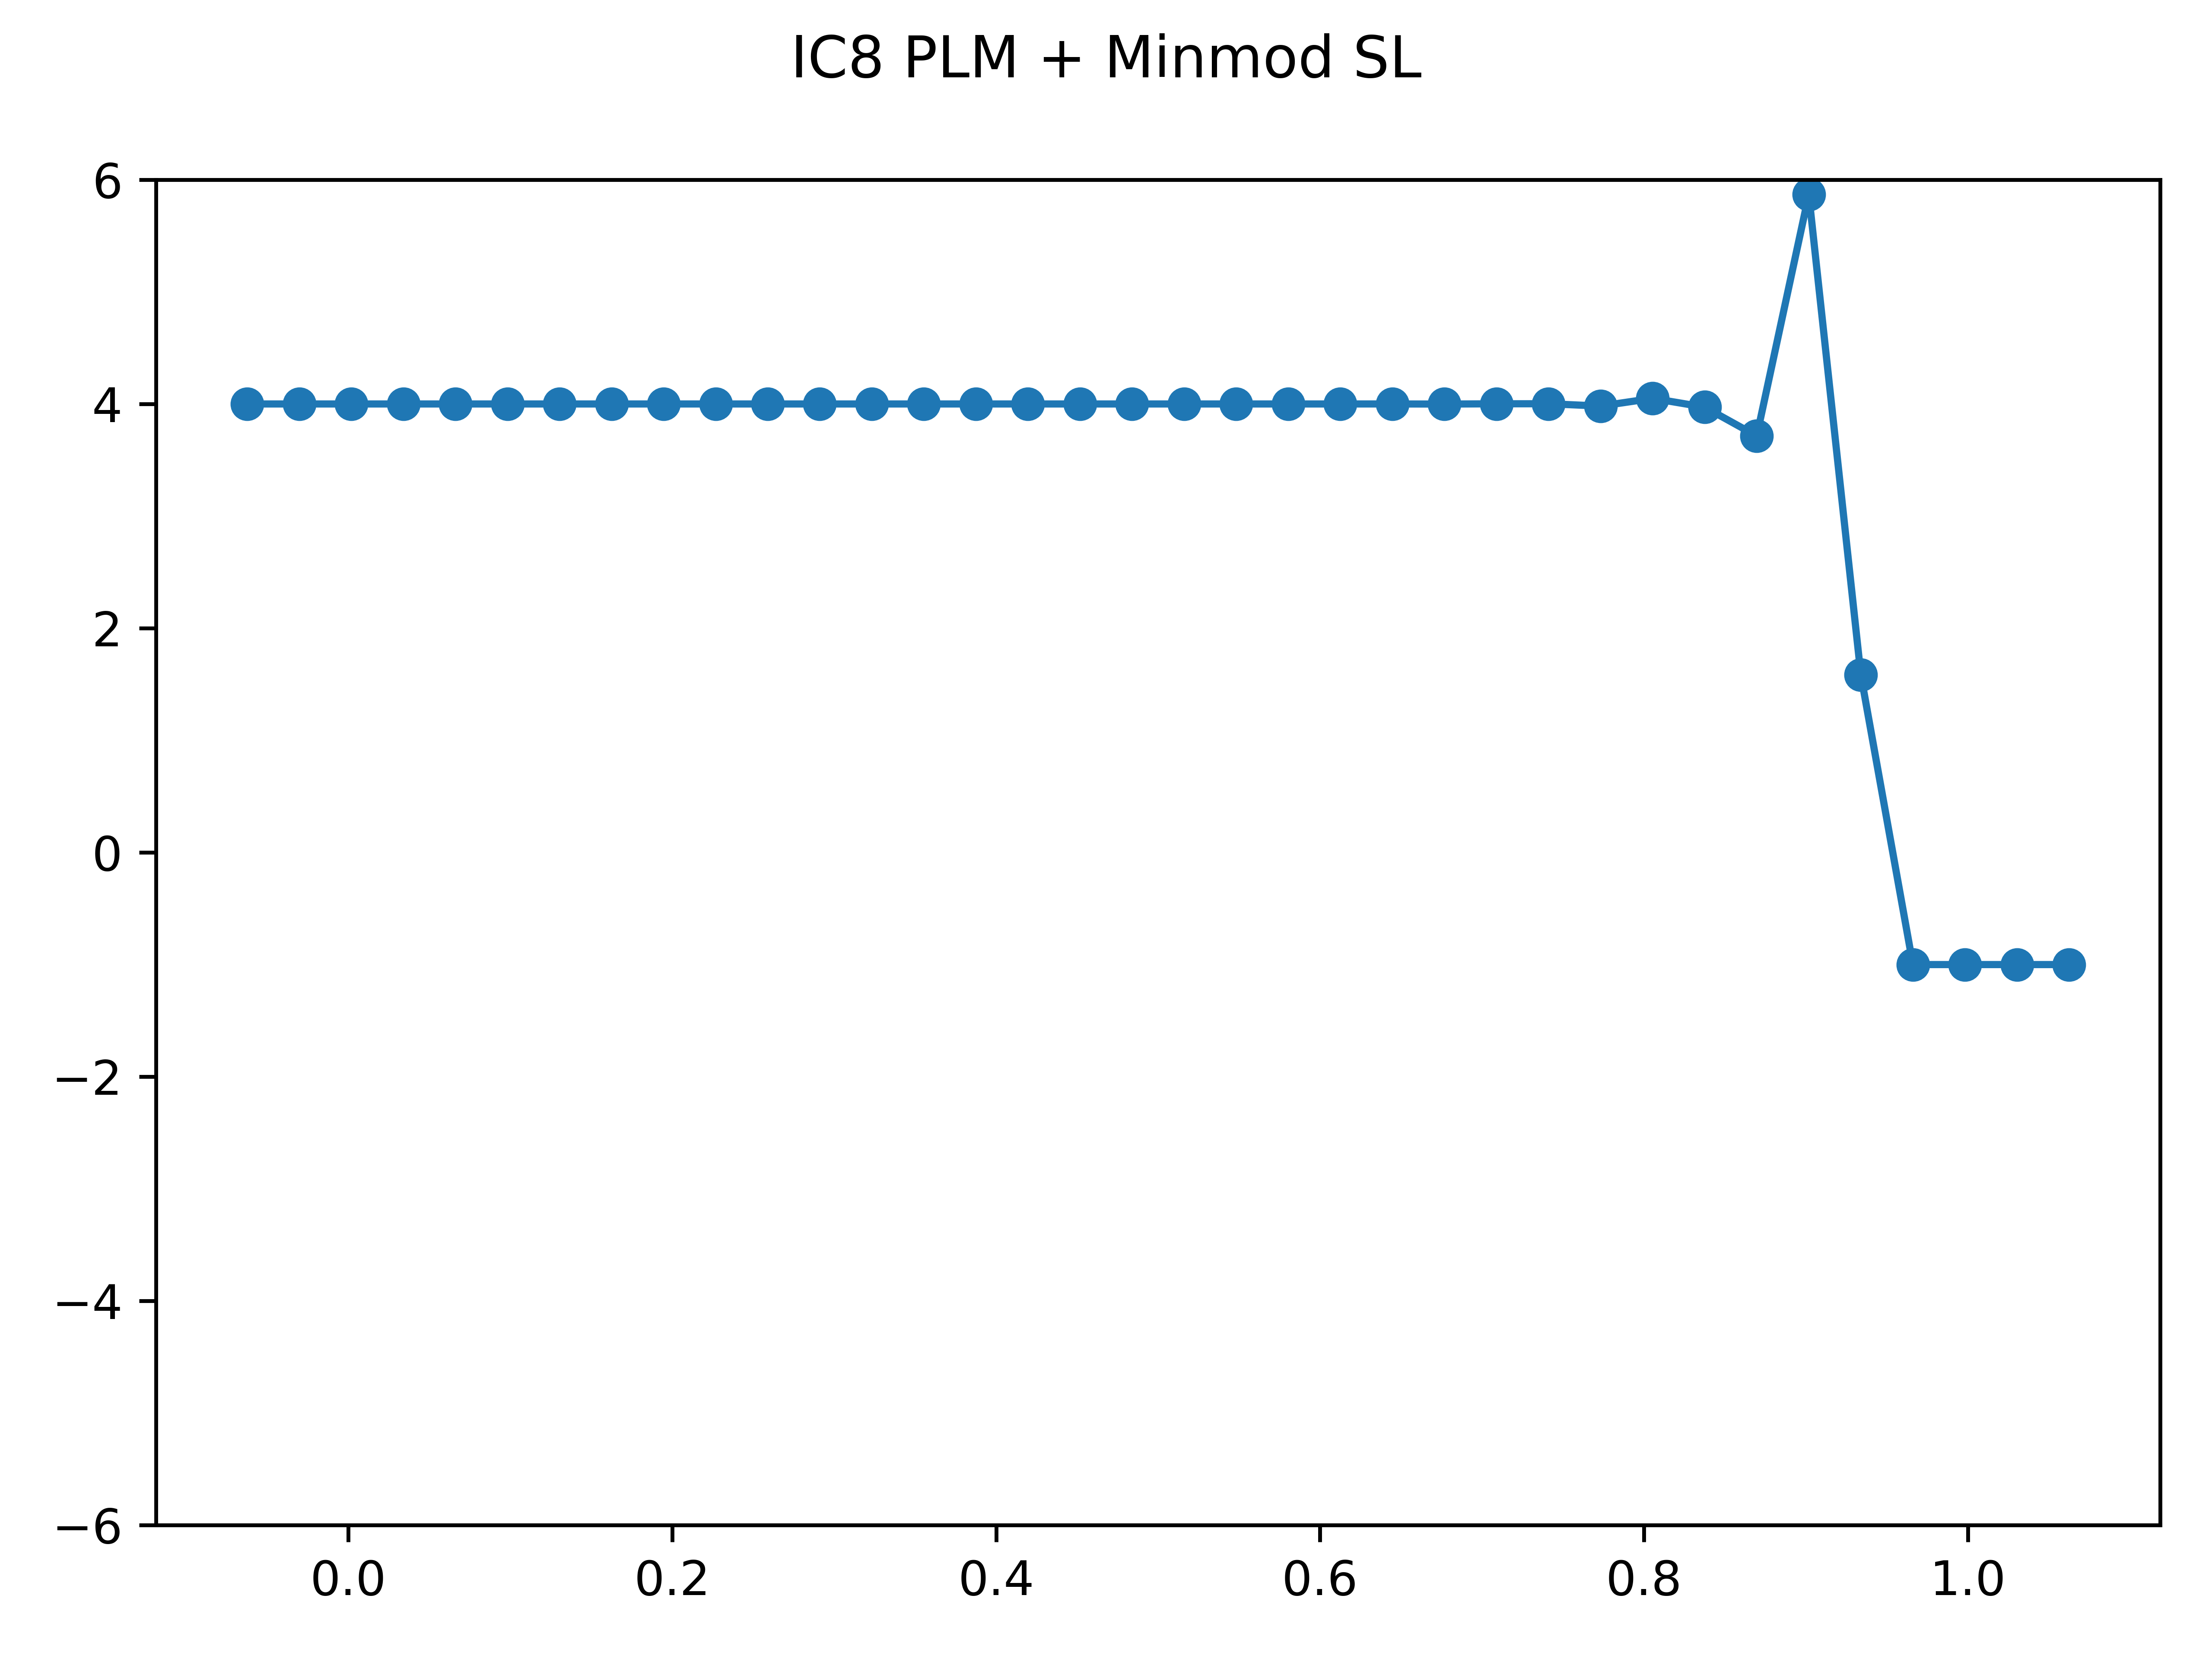
\includegraphics[width=.95\textwidth]{../../code/IC8Methodpm_plot.png}
        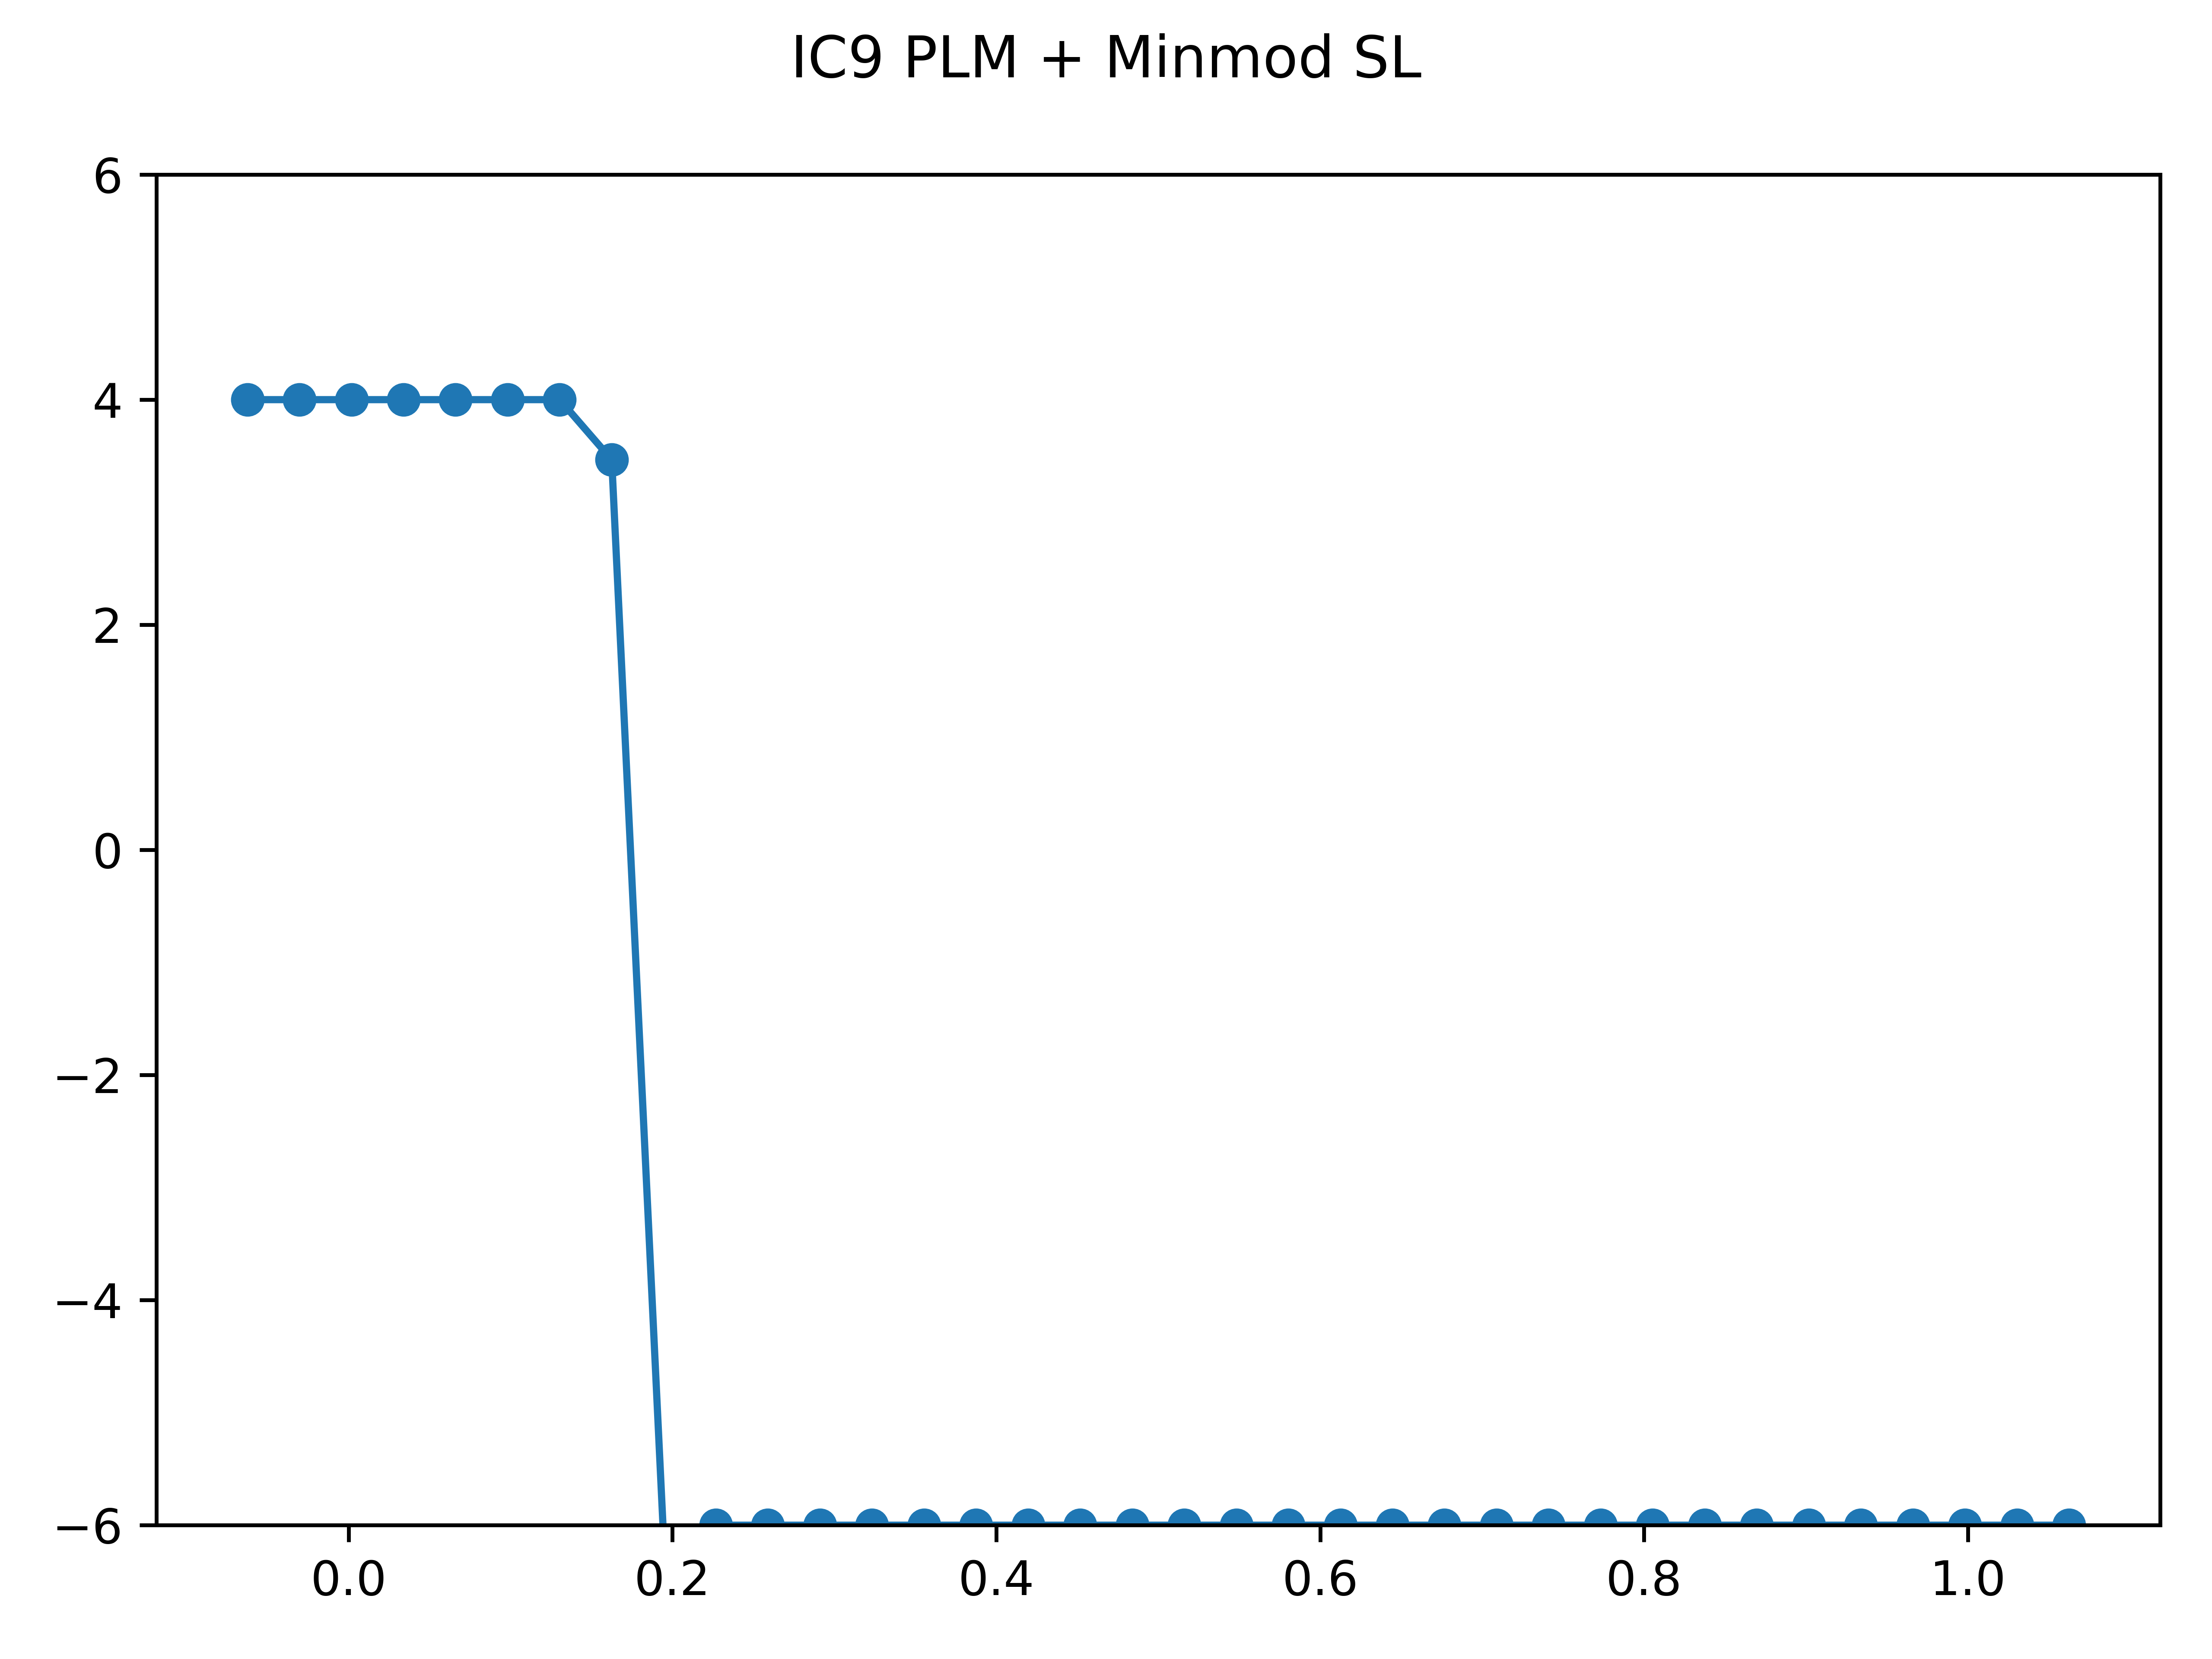
\includegraphics[width=.95\textwidth]{../../code/IC9Methodpm_plot.png}
        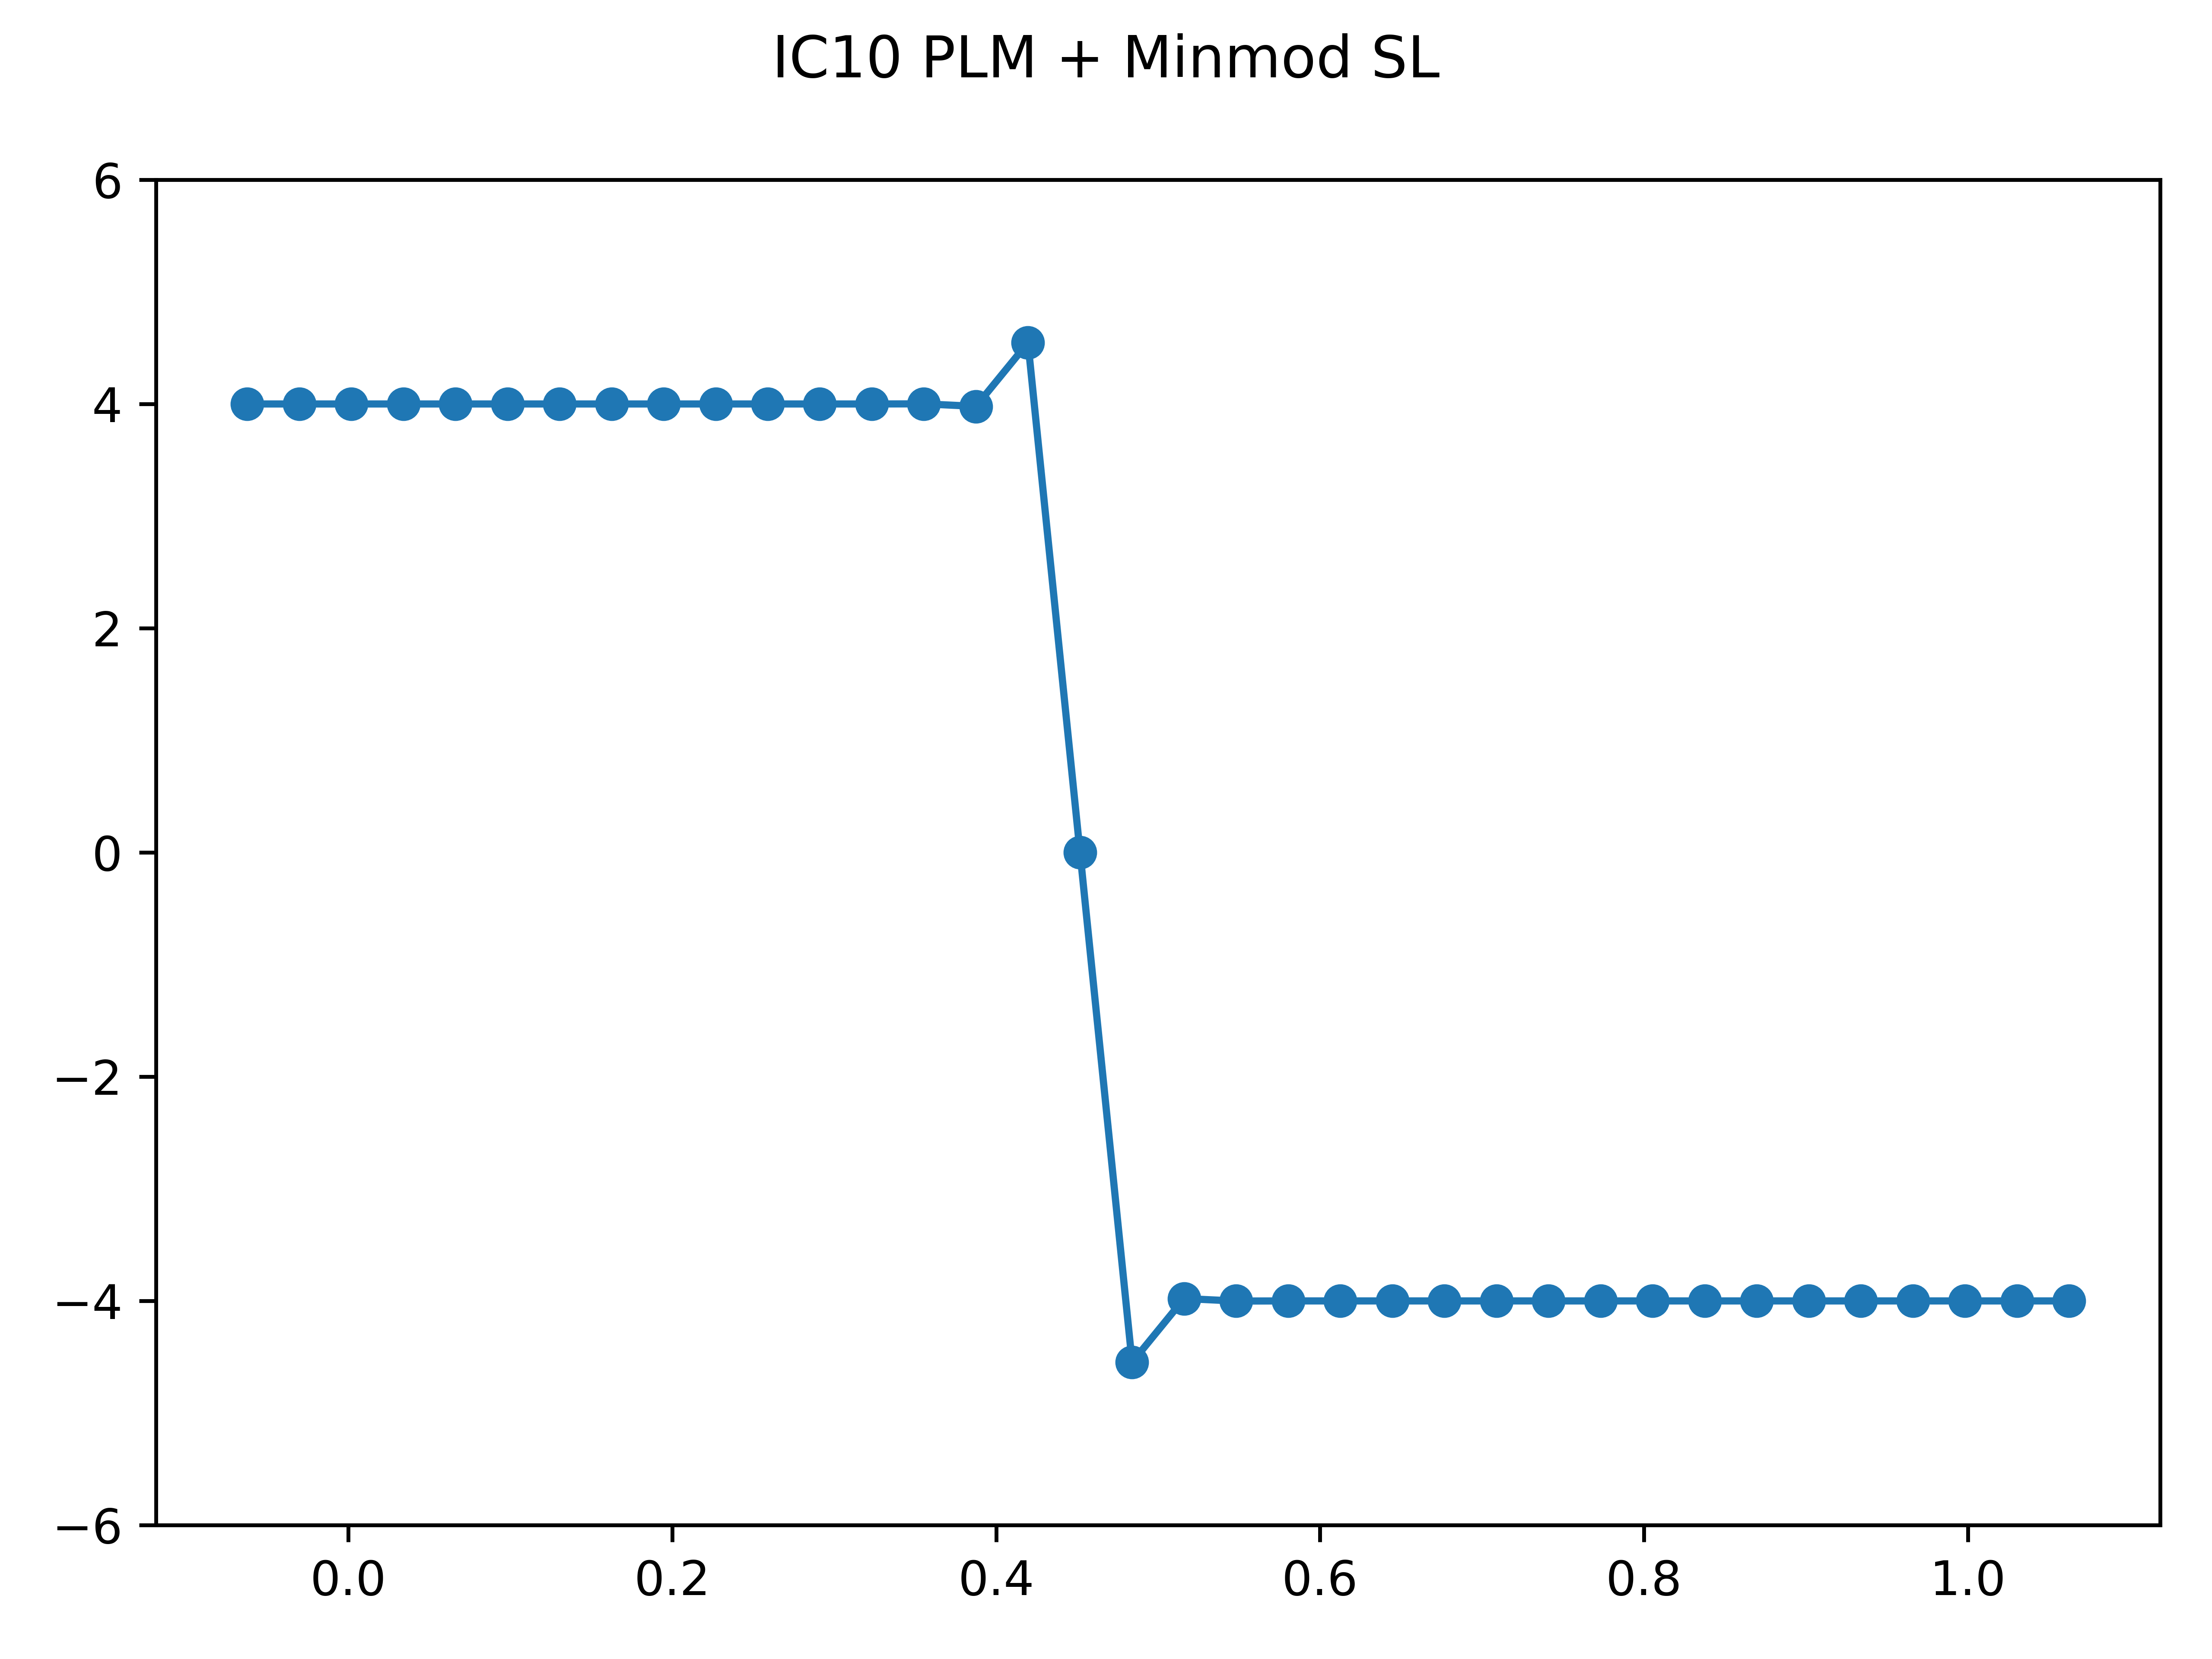
\includegraphics[width=.95\textwidth]{../../code/IC10Methodpm_plot.png}
        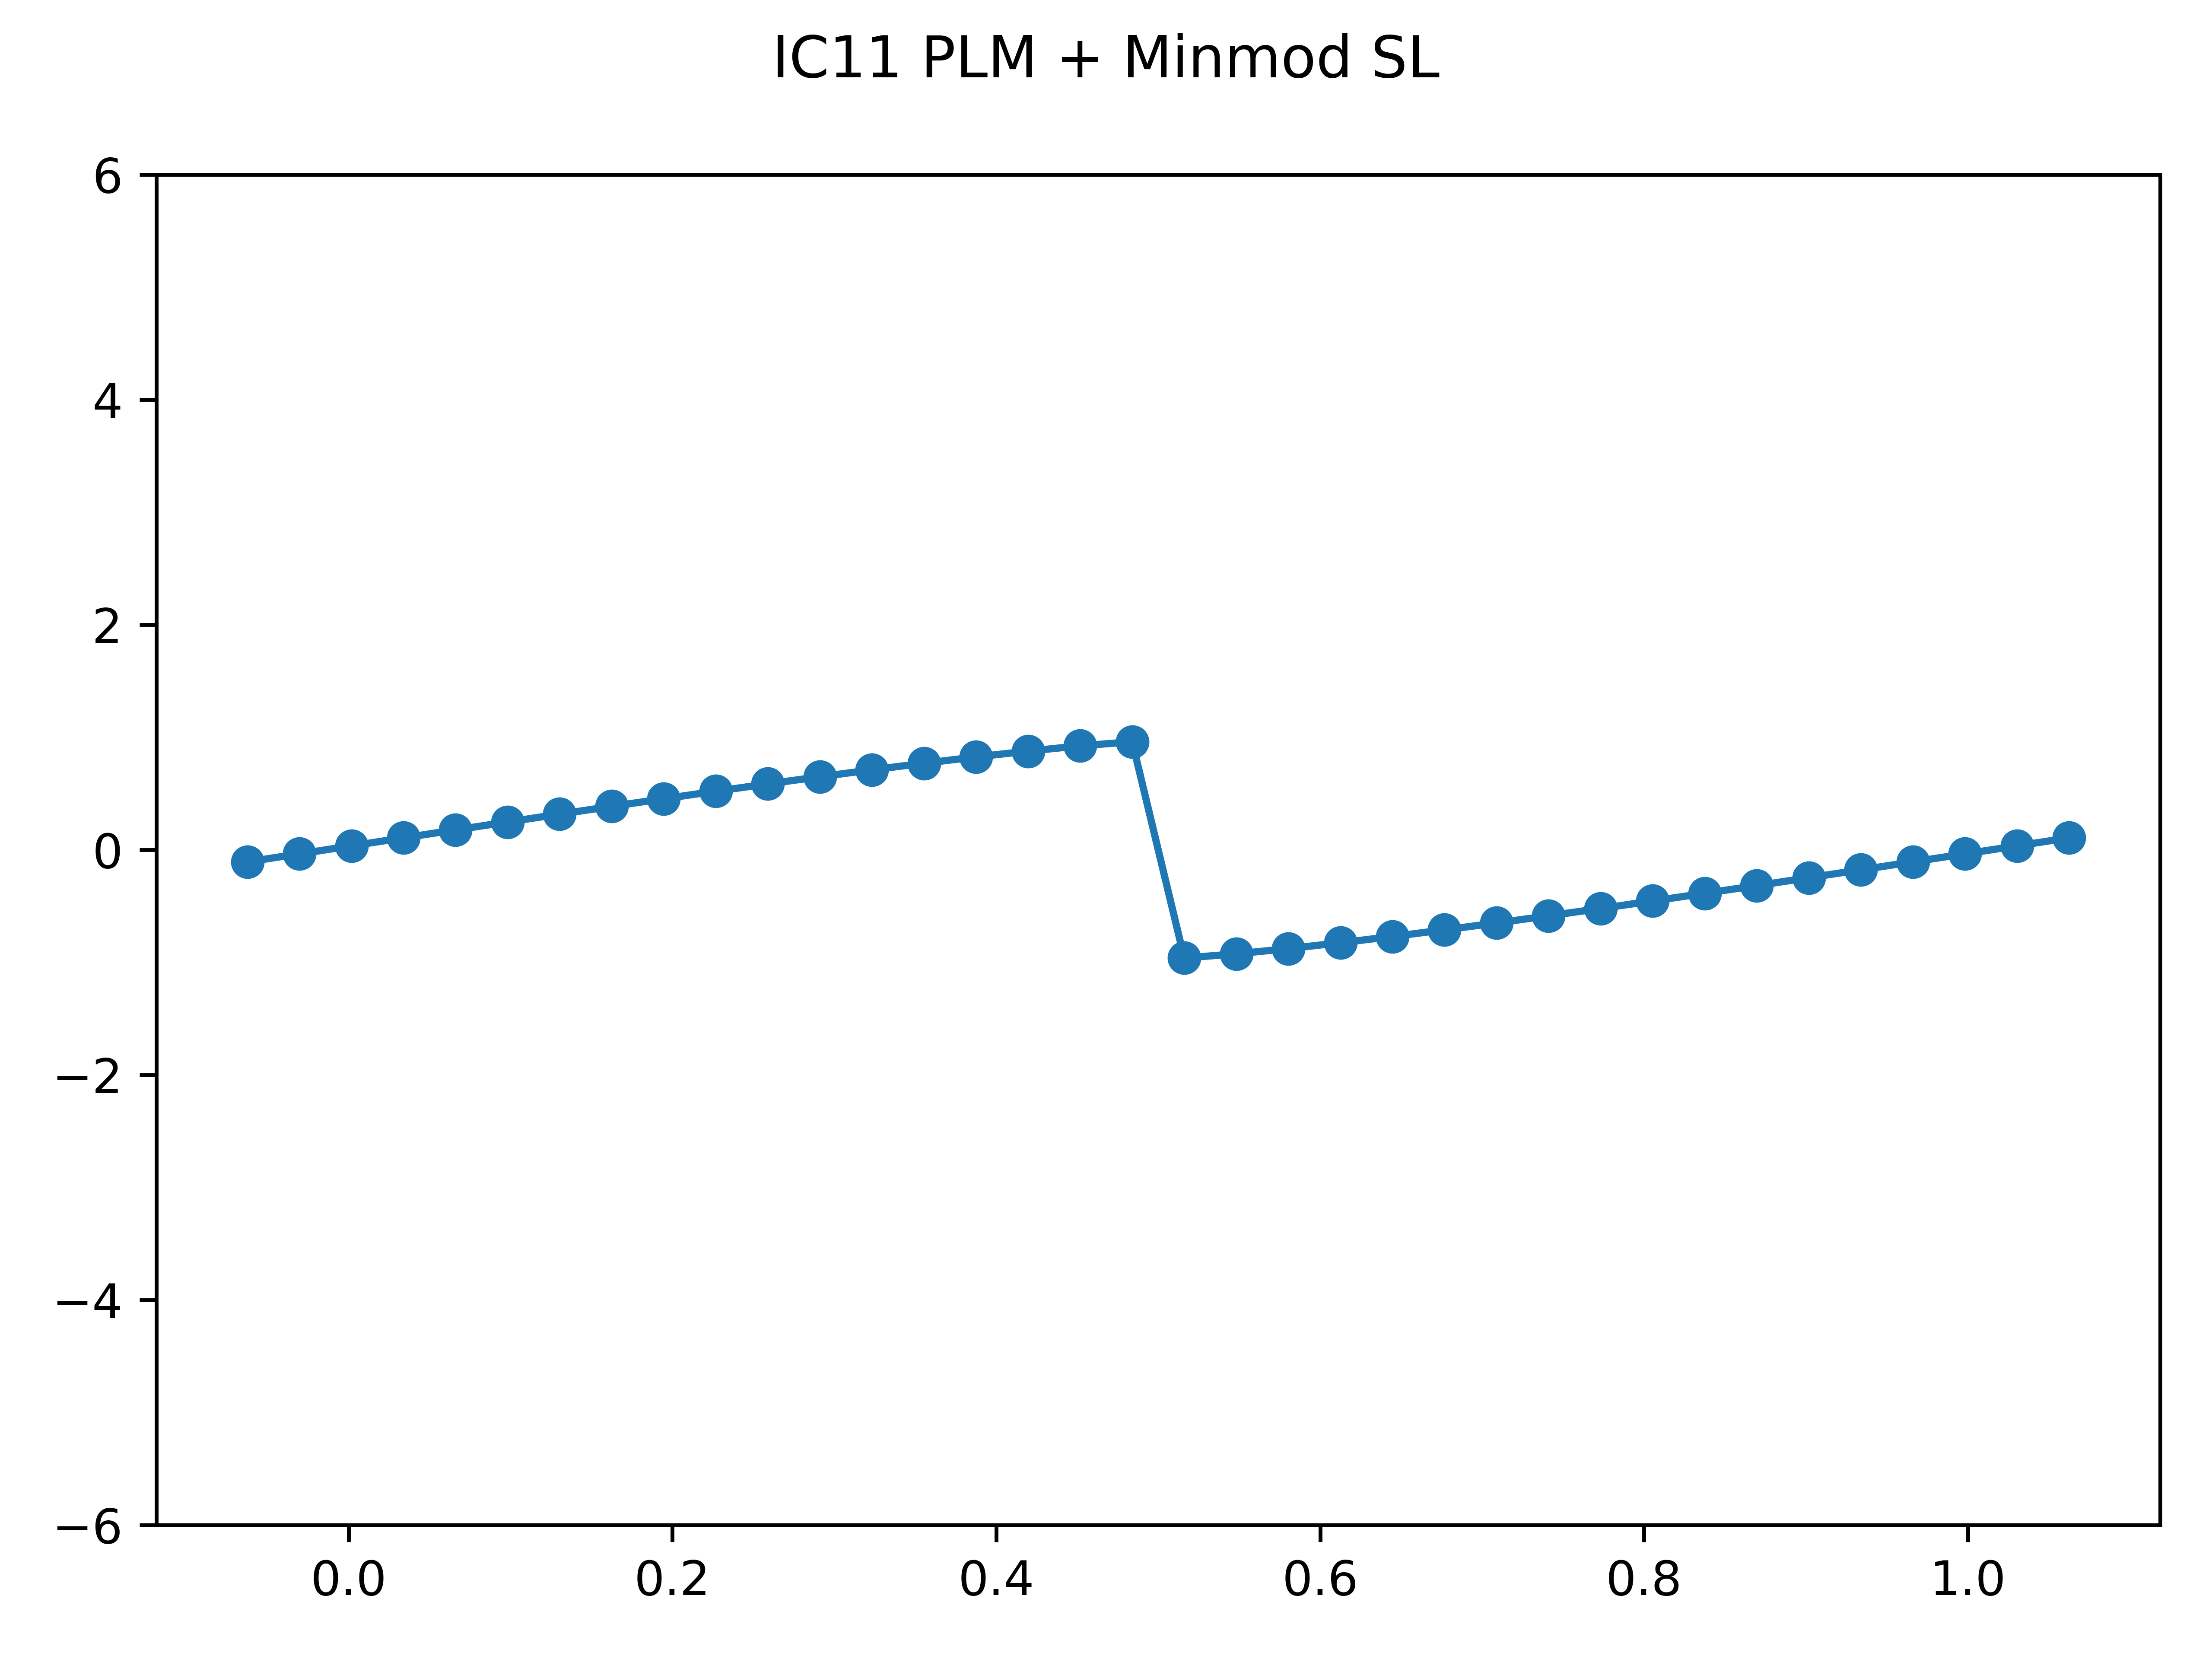
\includegraphics[width=.95\textwidth]{../../code/IC11Methodpm_plot.png}
    \emp
    \bmp{0.25}
        \centering
        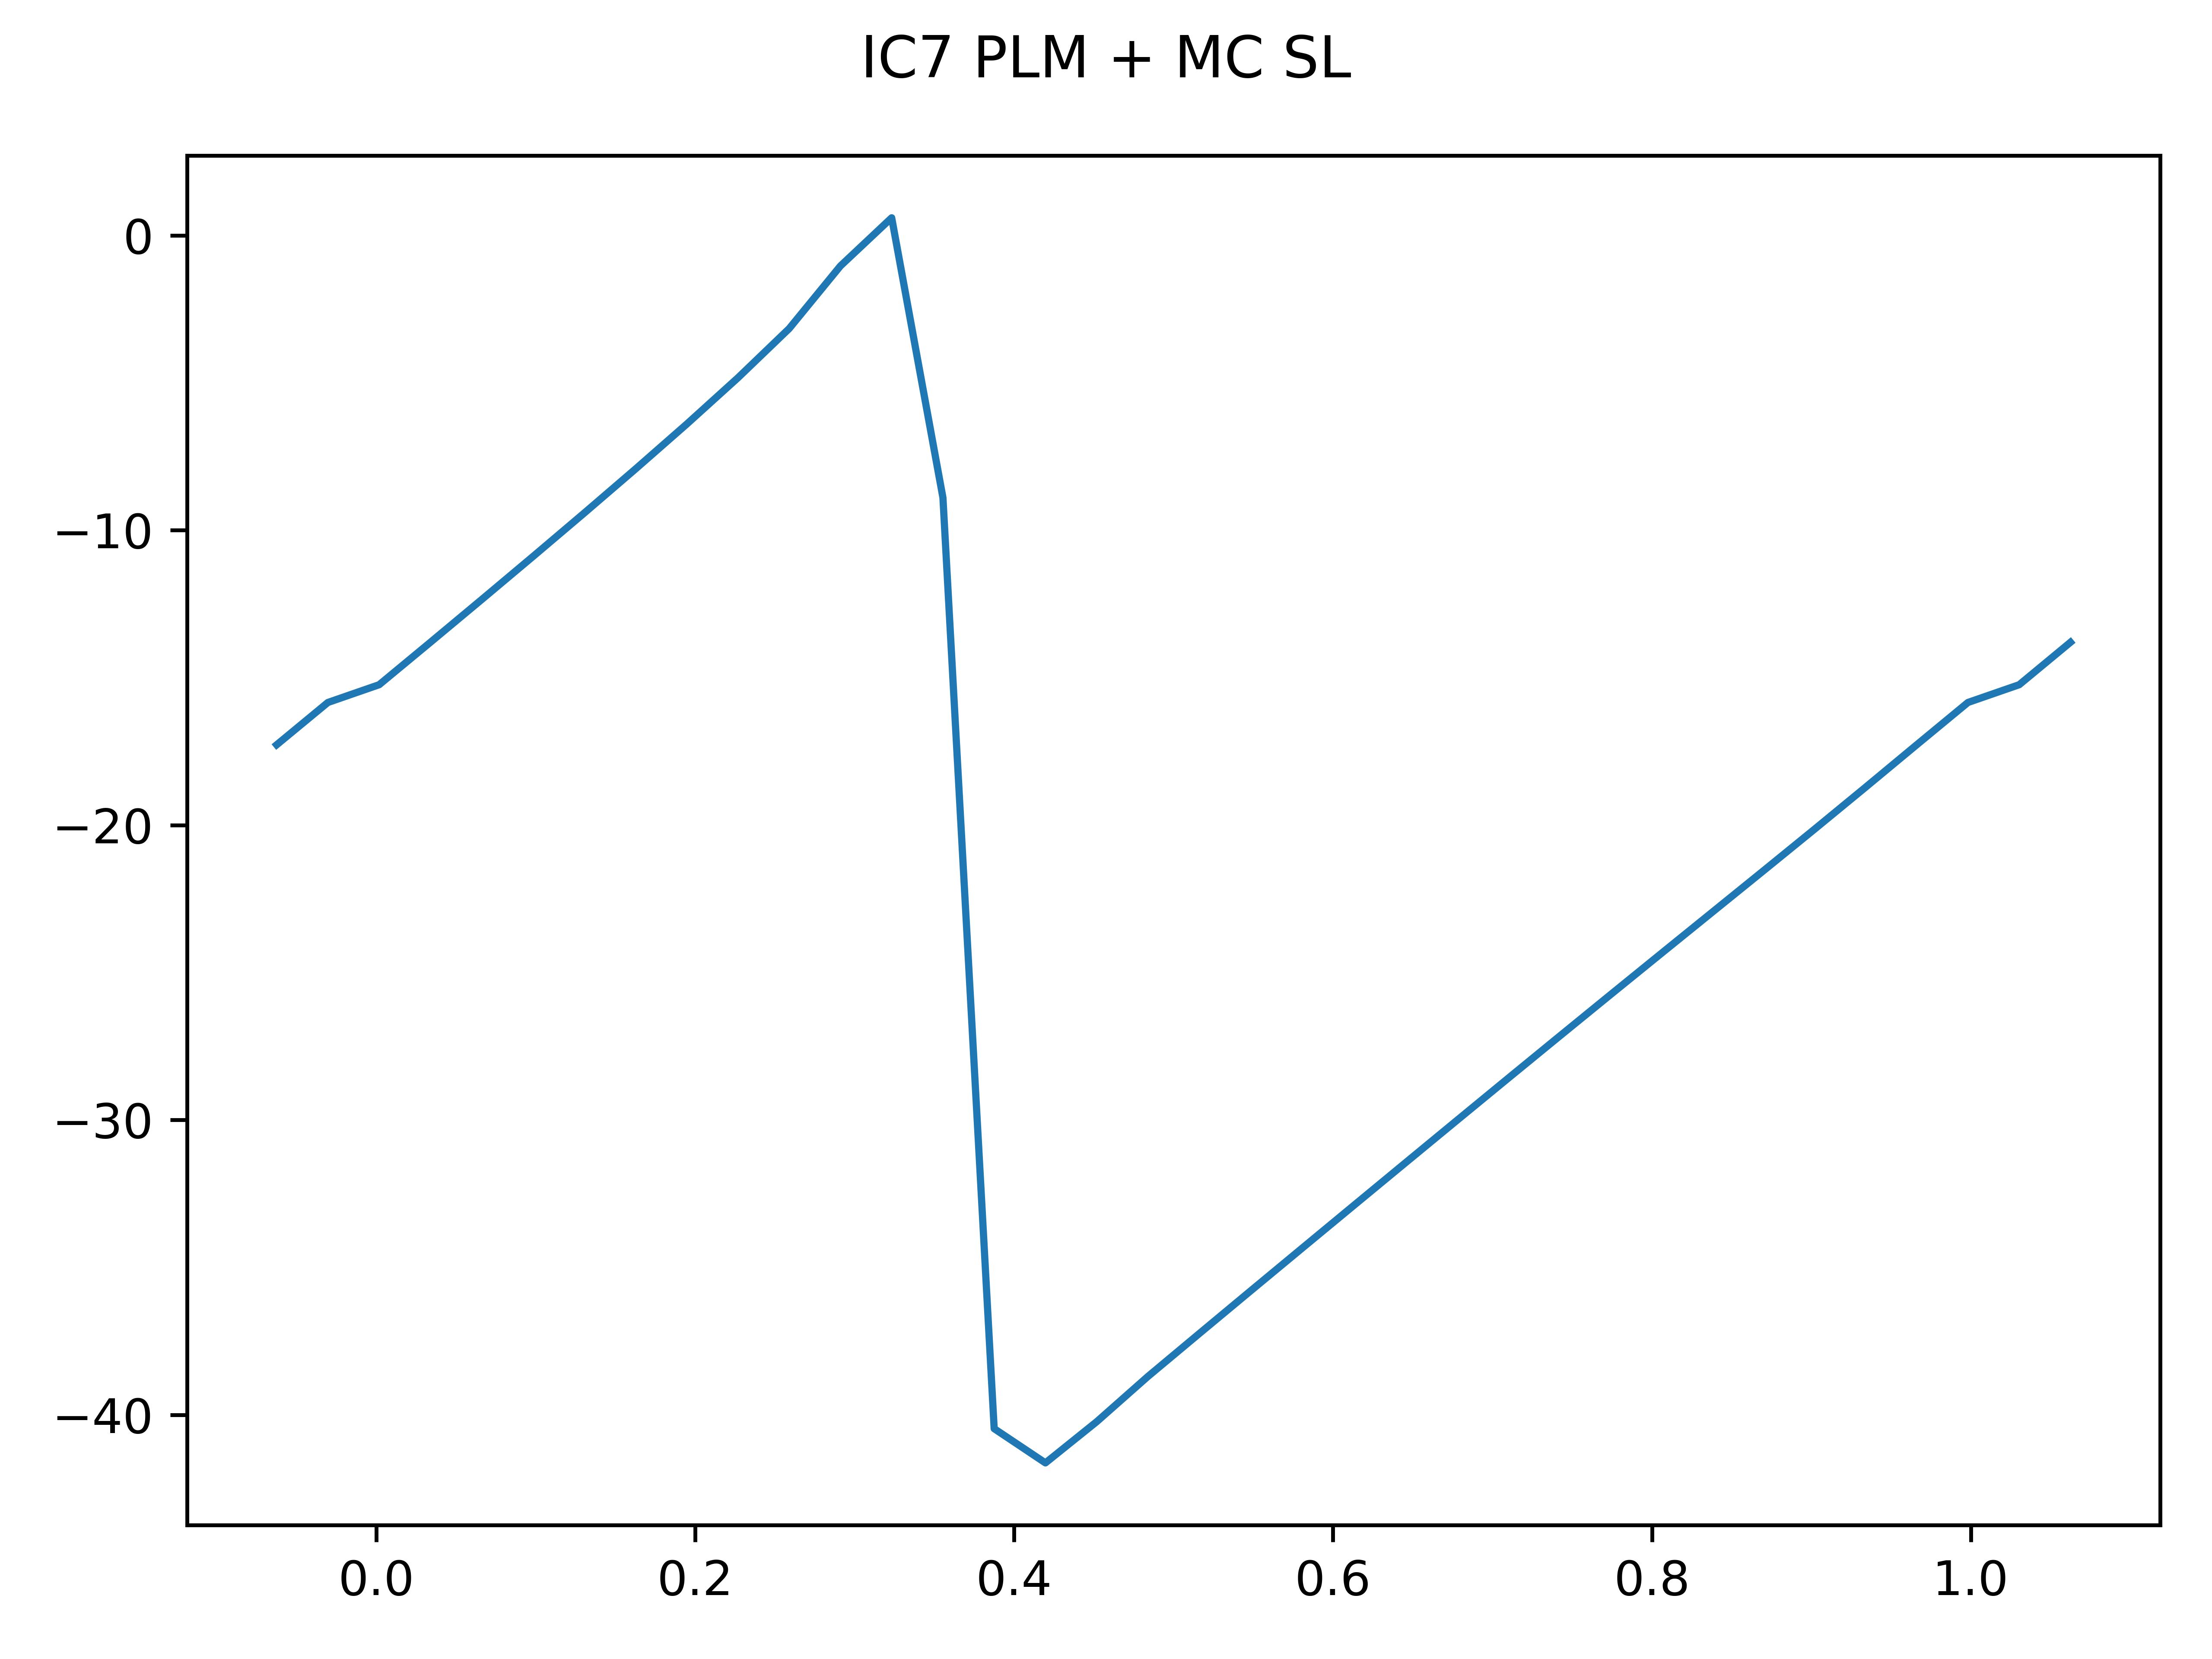
\includegraphics[width=.95\textwidth]{../../code/IC7Methodpo_plot.png}
        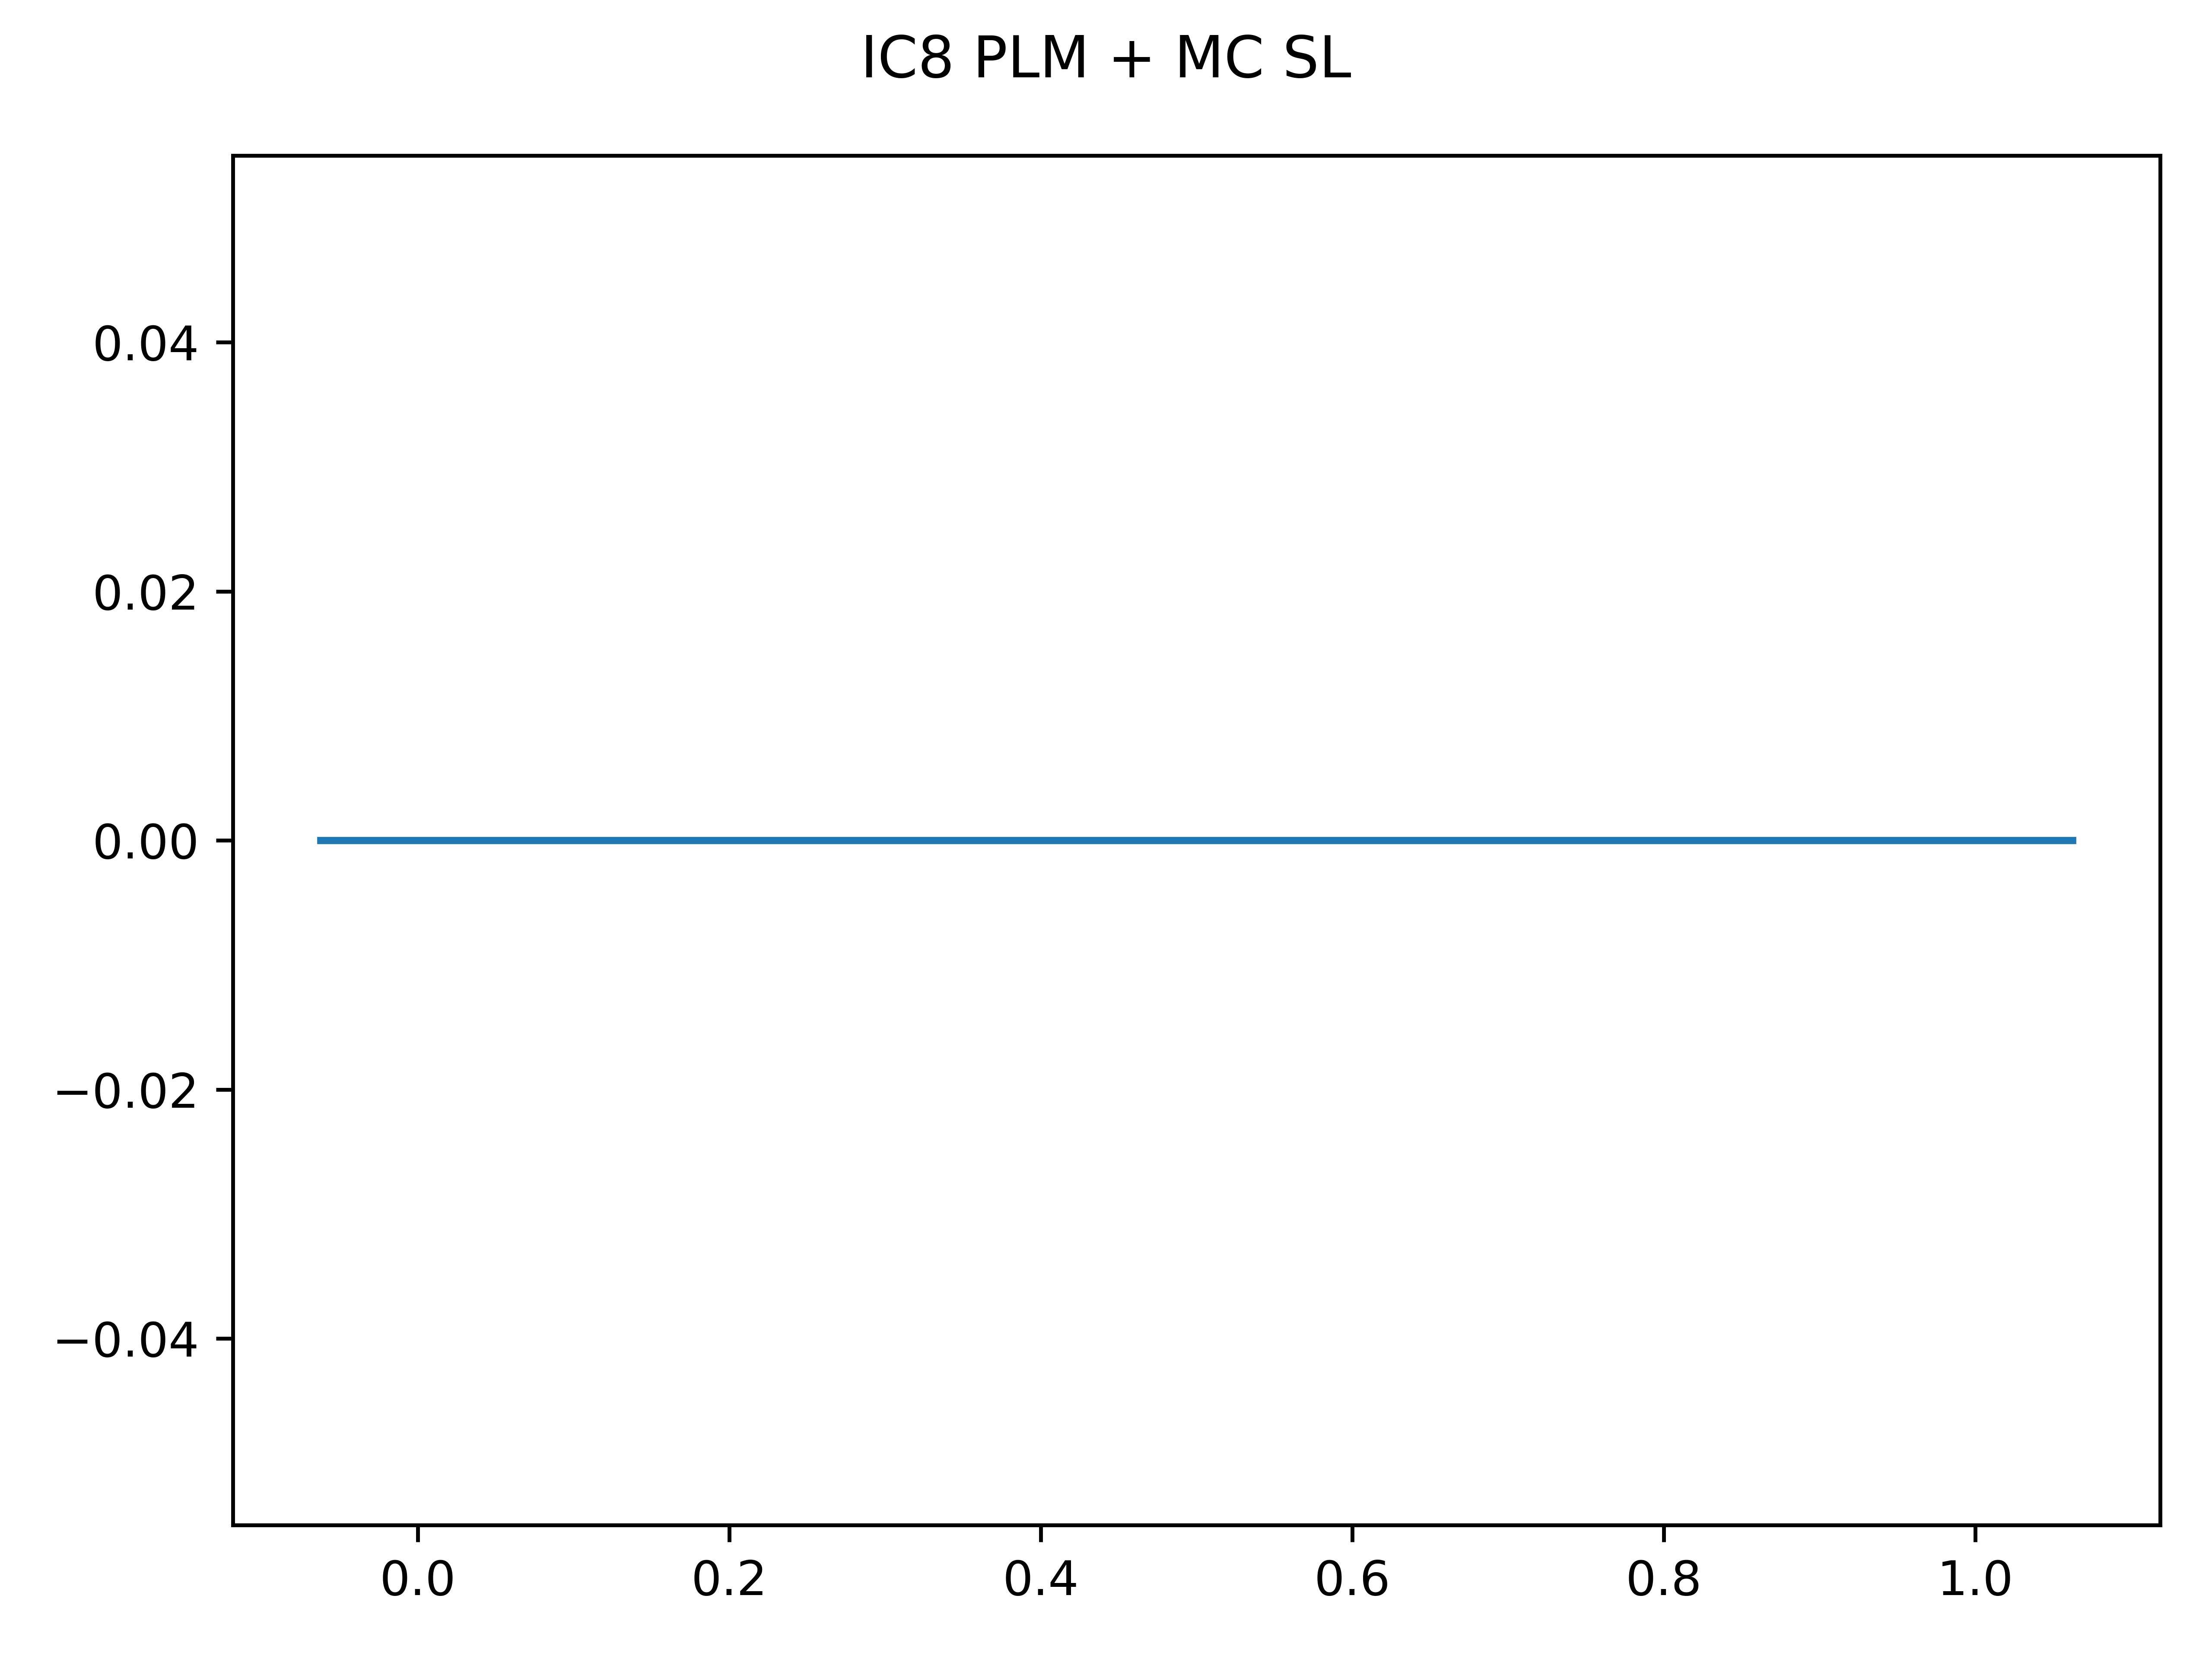
\includegraphics[width=.95\textwidth]{../../code/IC8Methodpo_plot.png}
        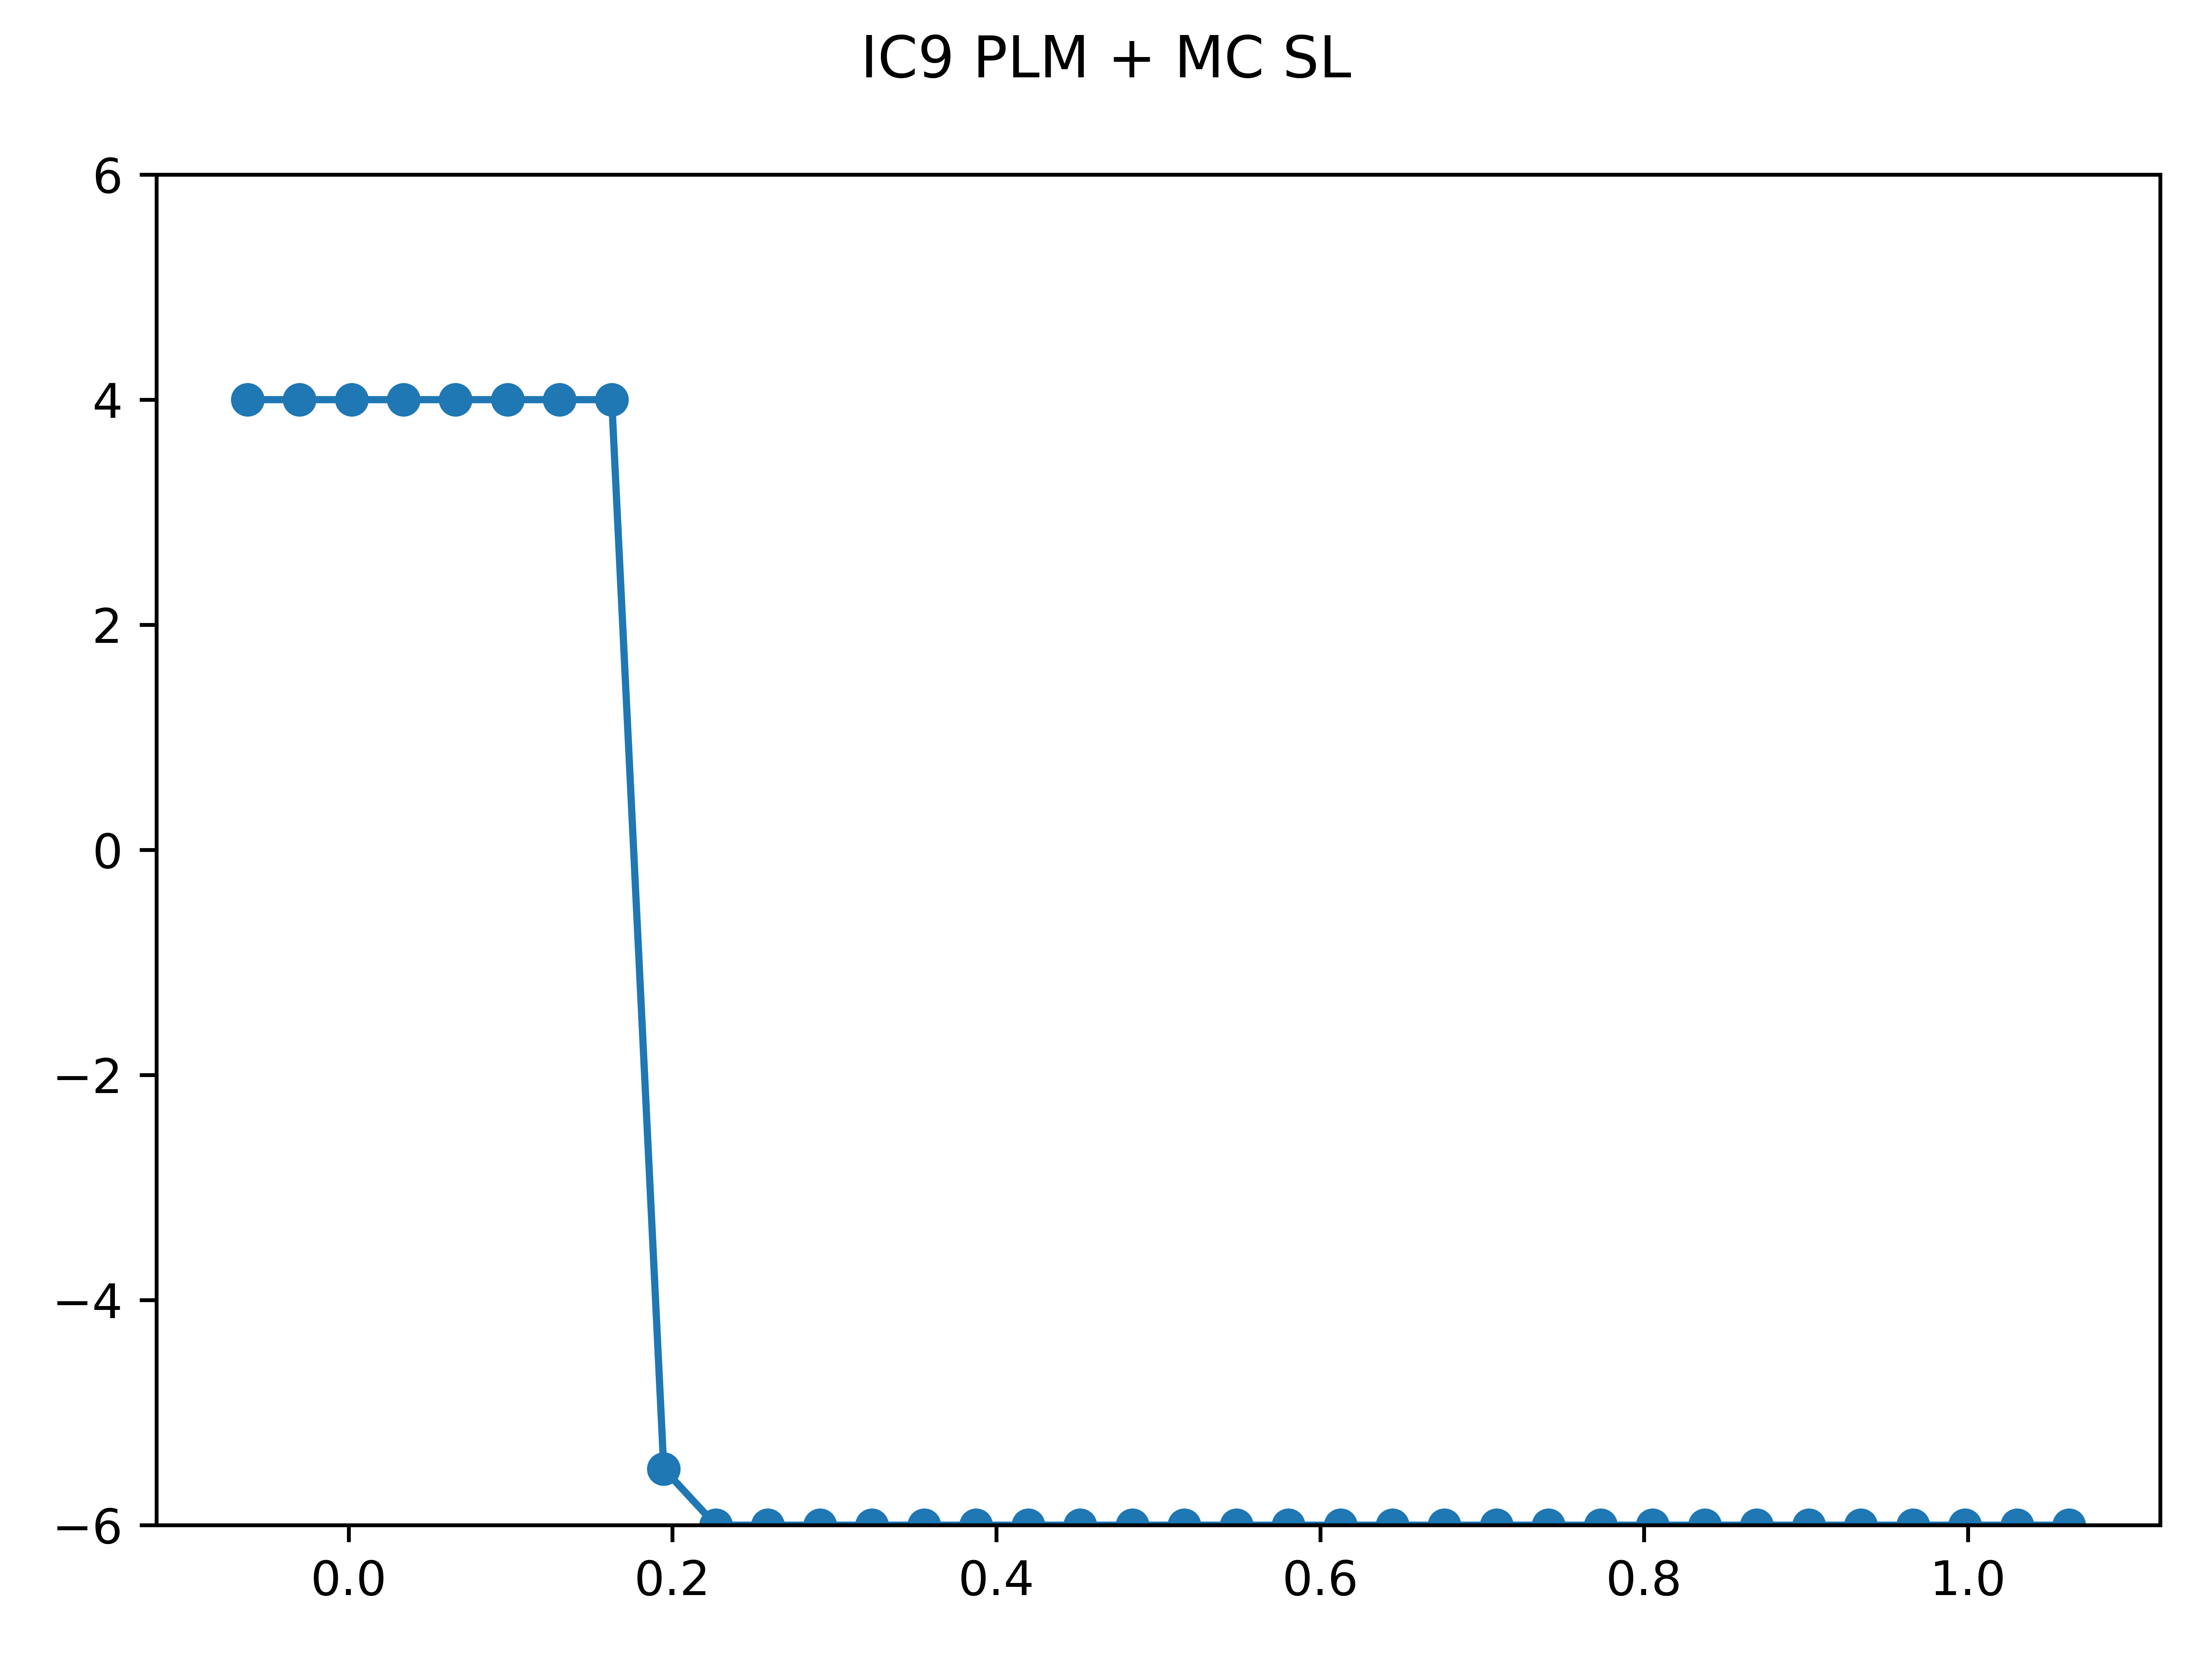
\includegraphics[width=.95\textwidth]{../../code/IC9Methodpo_plot.png}
        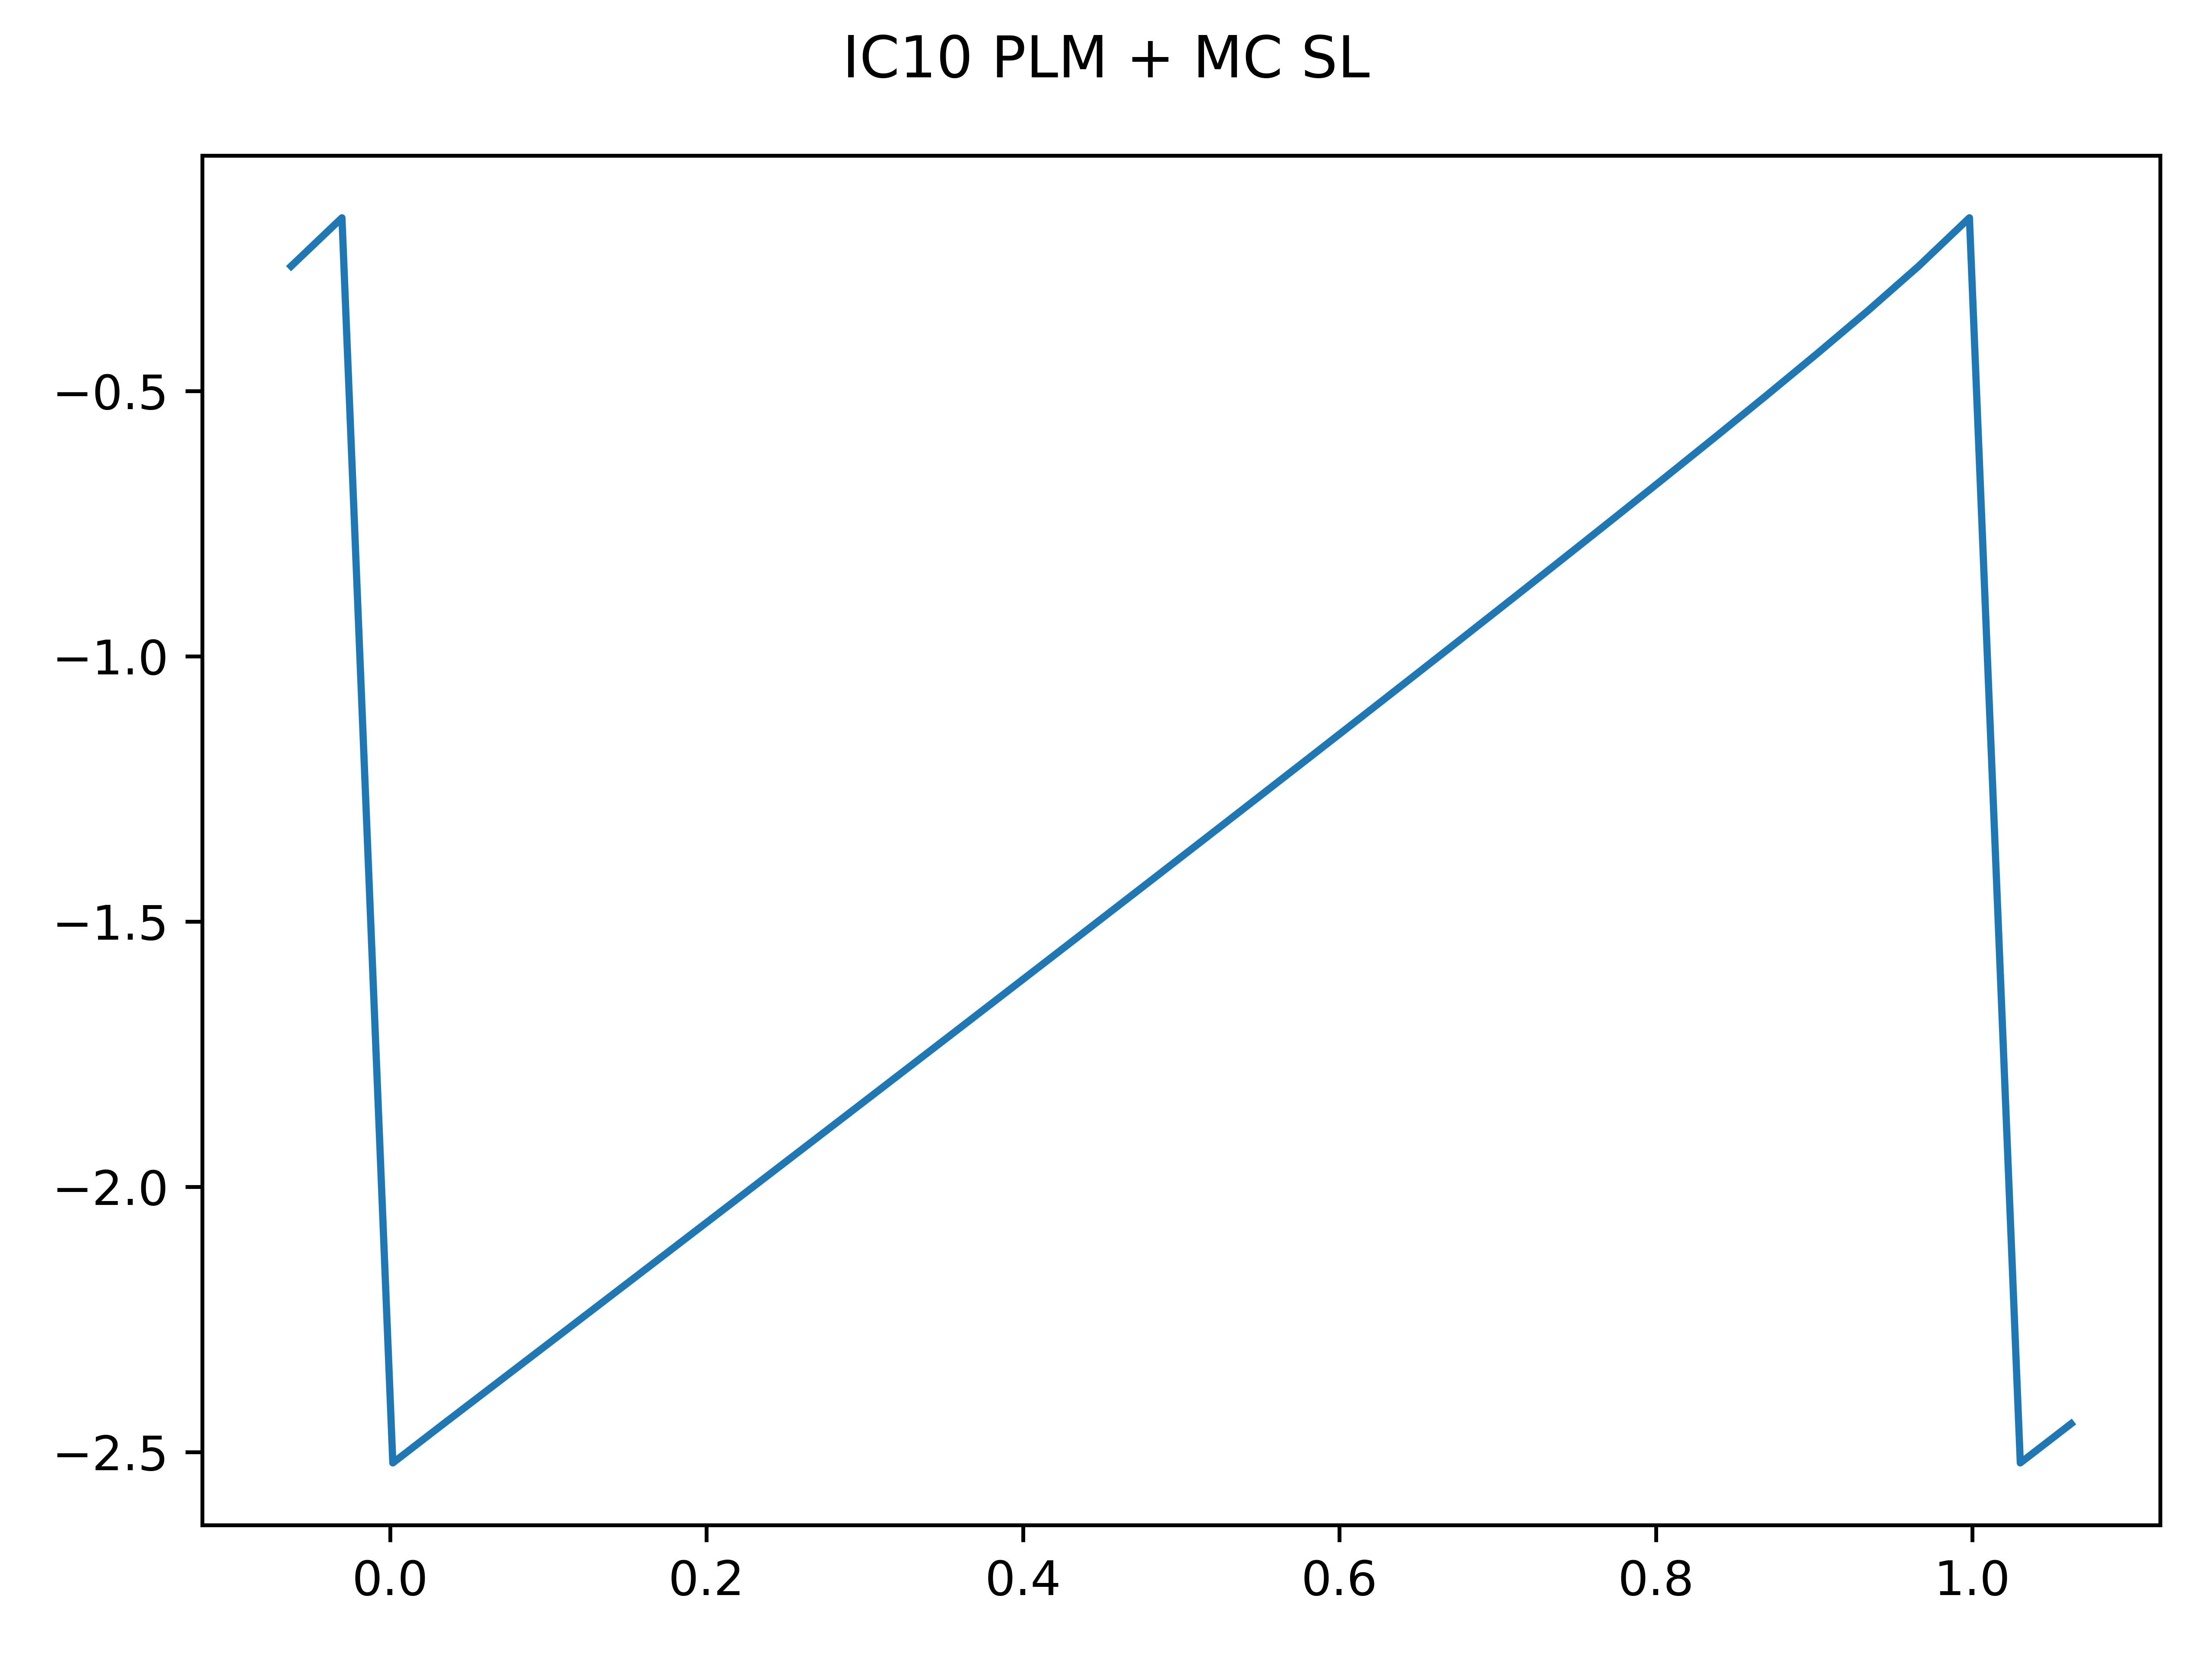
\includegraphics[width=.95\textwidth]{../../code/IC10Methodpo_plot.png}
        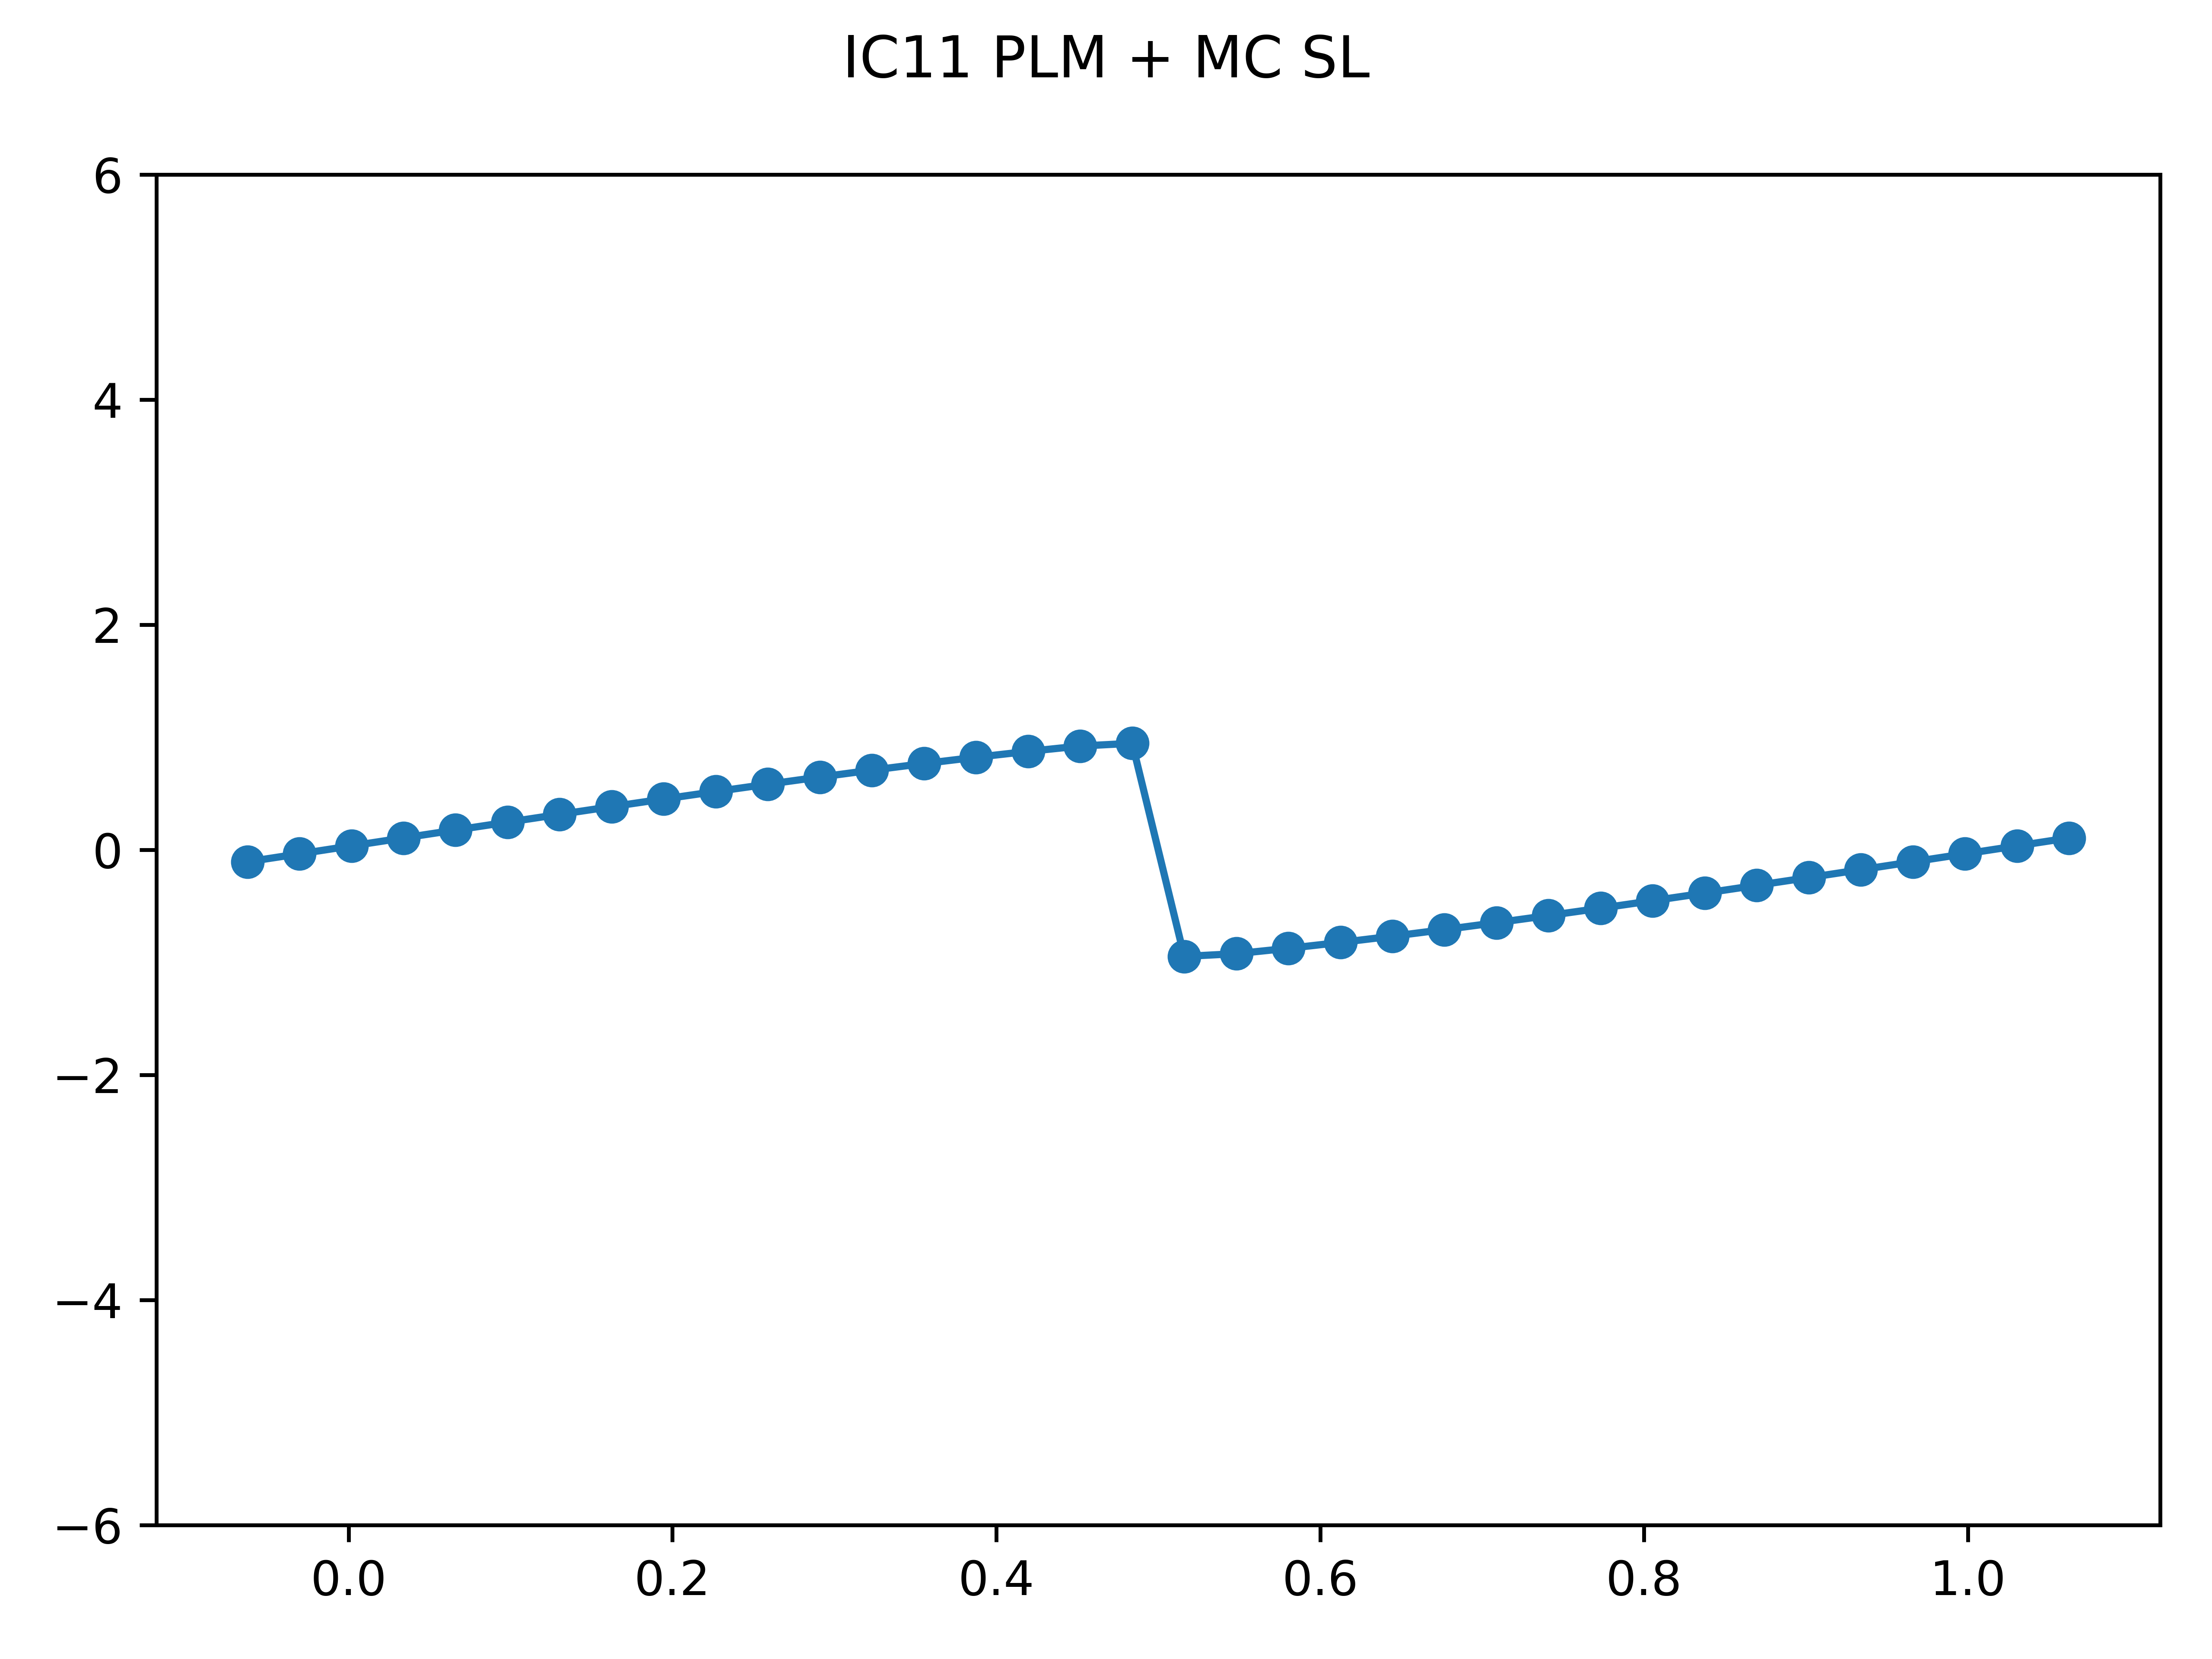
\includegraphics[width=.95\textwidth]{../../code/IC11Methodpo_plot.png}
    \emp
    \bmp{0.25}
        \centering
        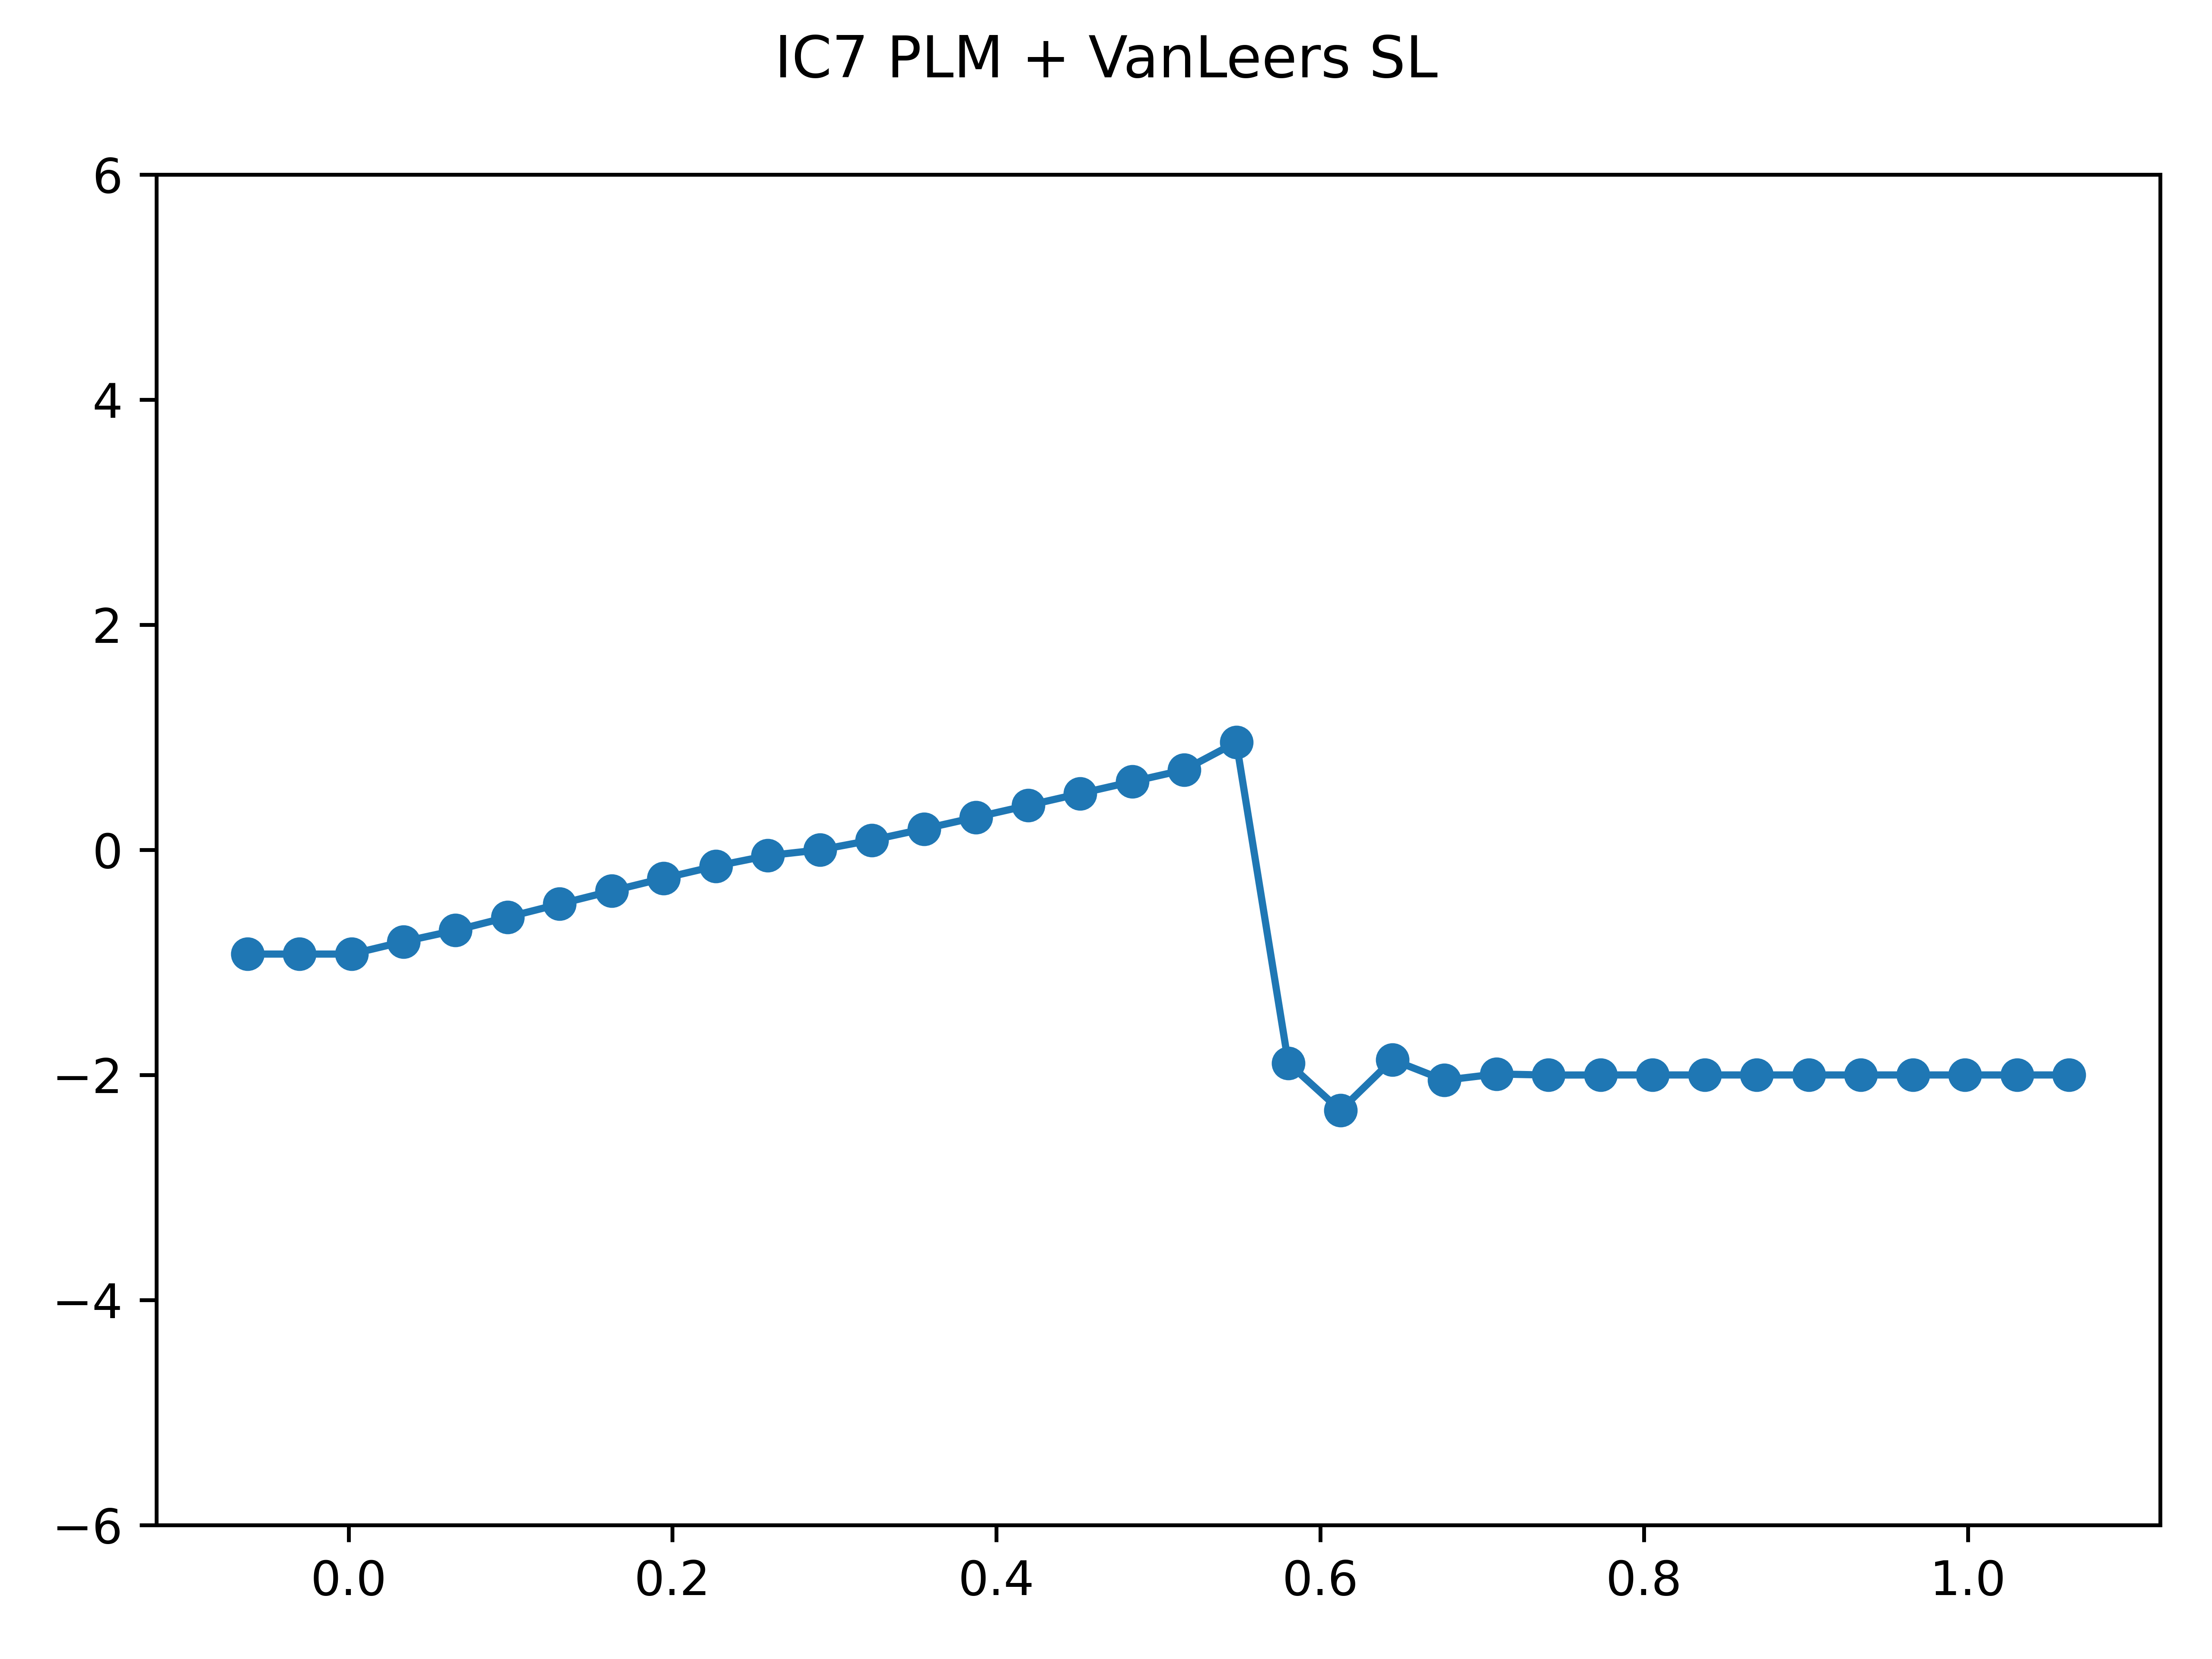
\includegraphics[width=.95\textwidth]{../../code/IC7Methodpv_plot.png}
        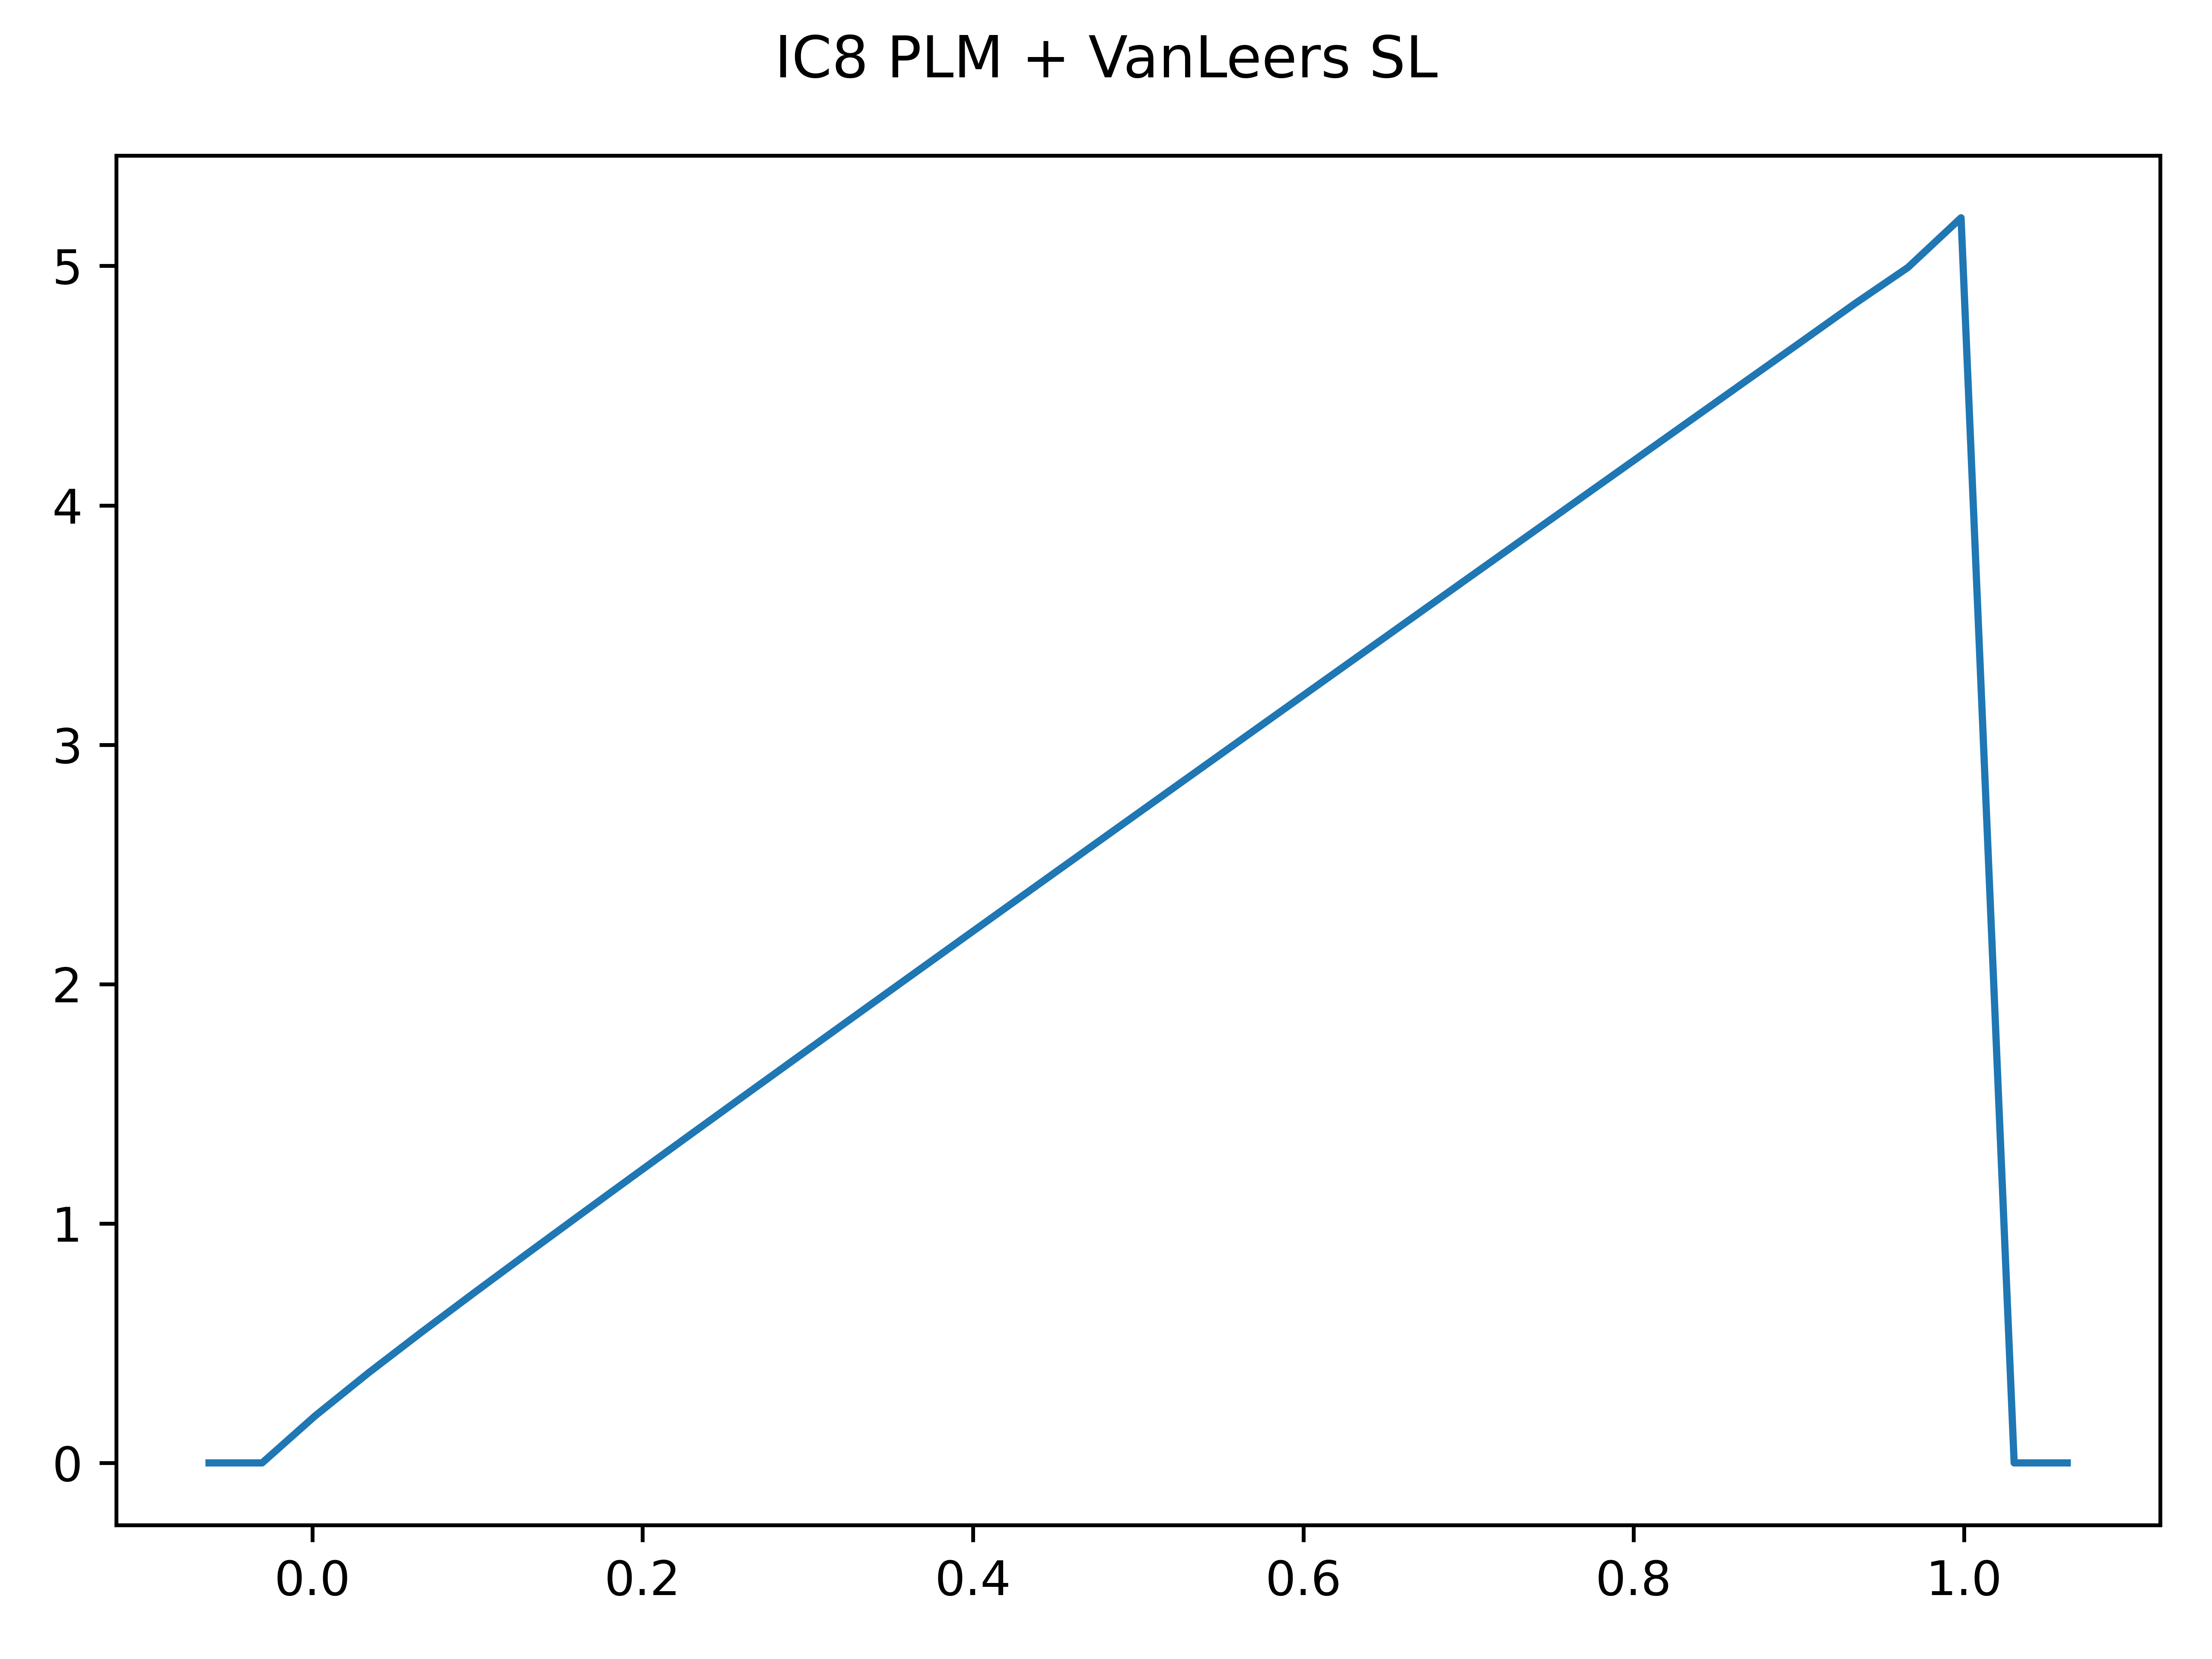
\includegraphics[width=.95\textwidth]{../../code/IC8Methodpv_plot.png}
        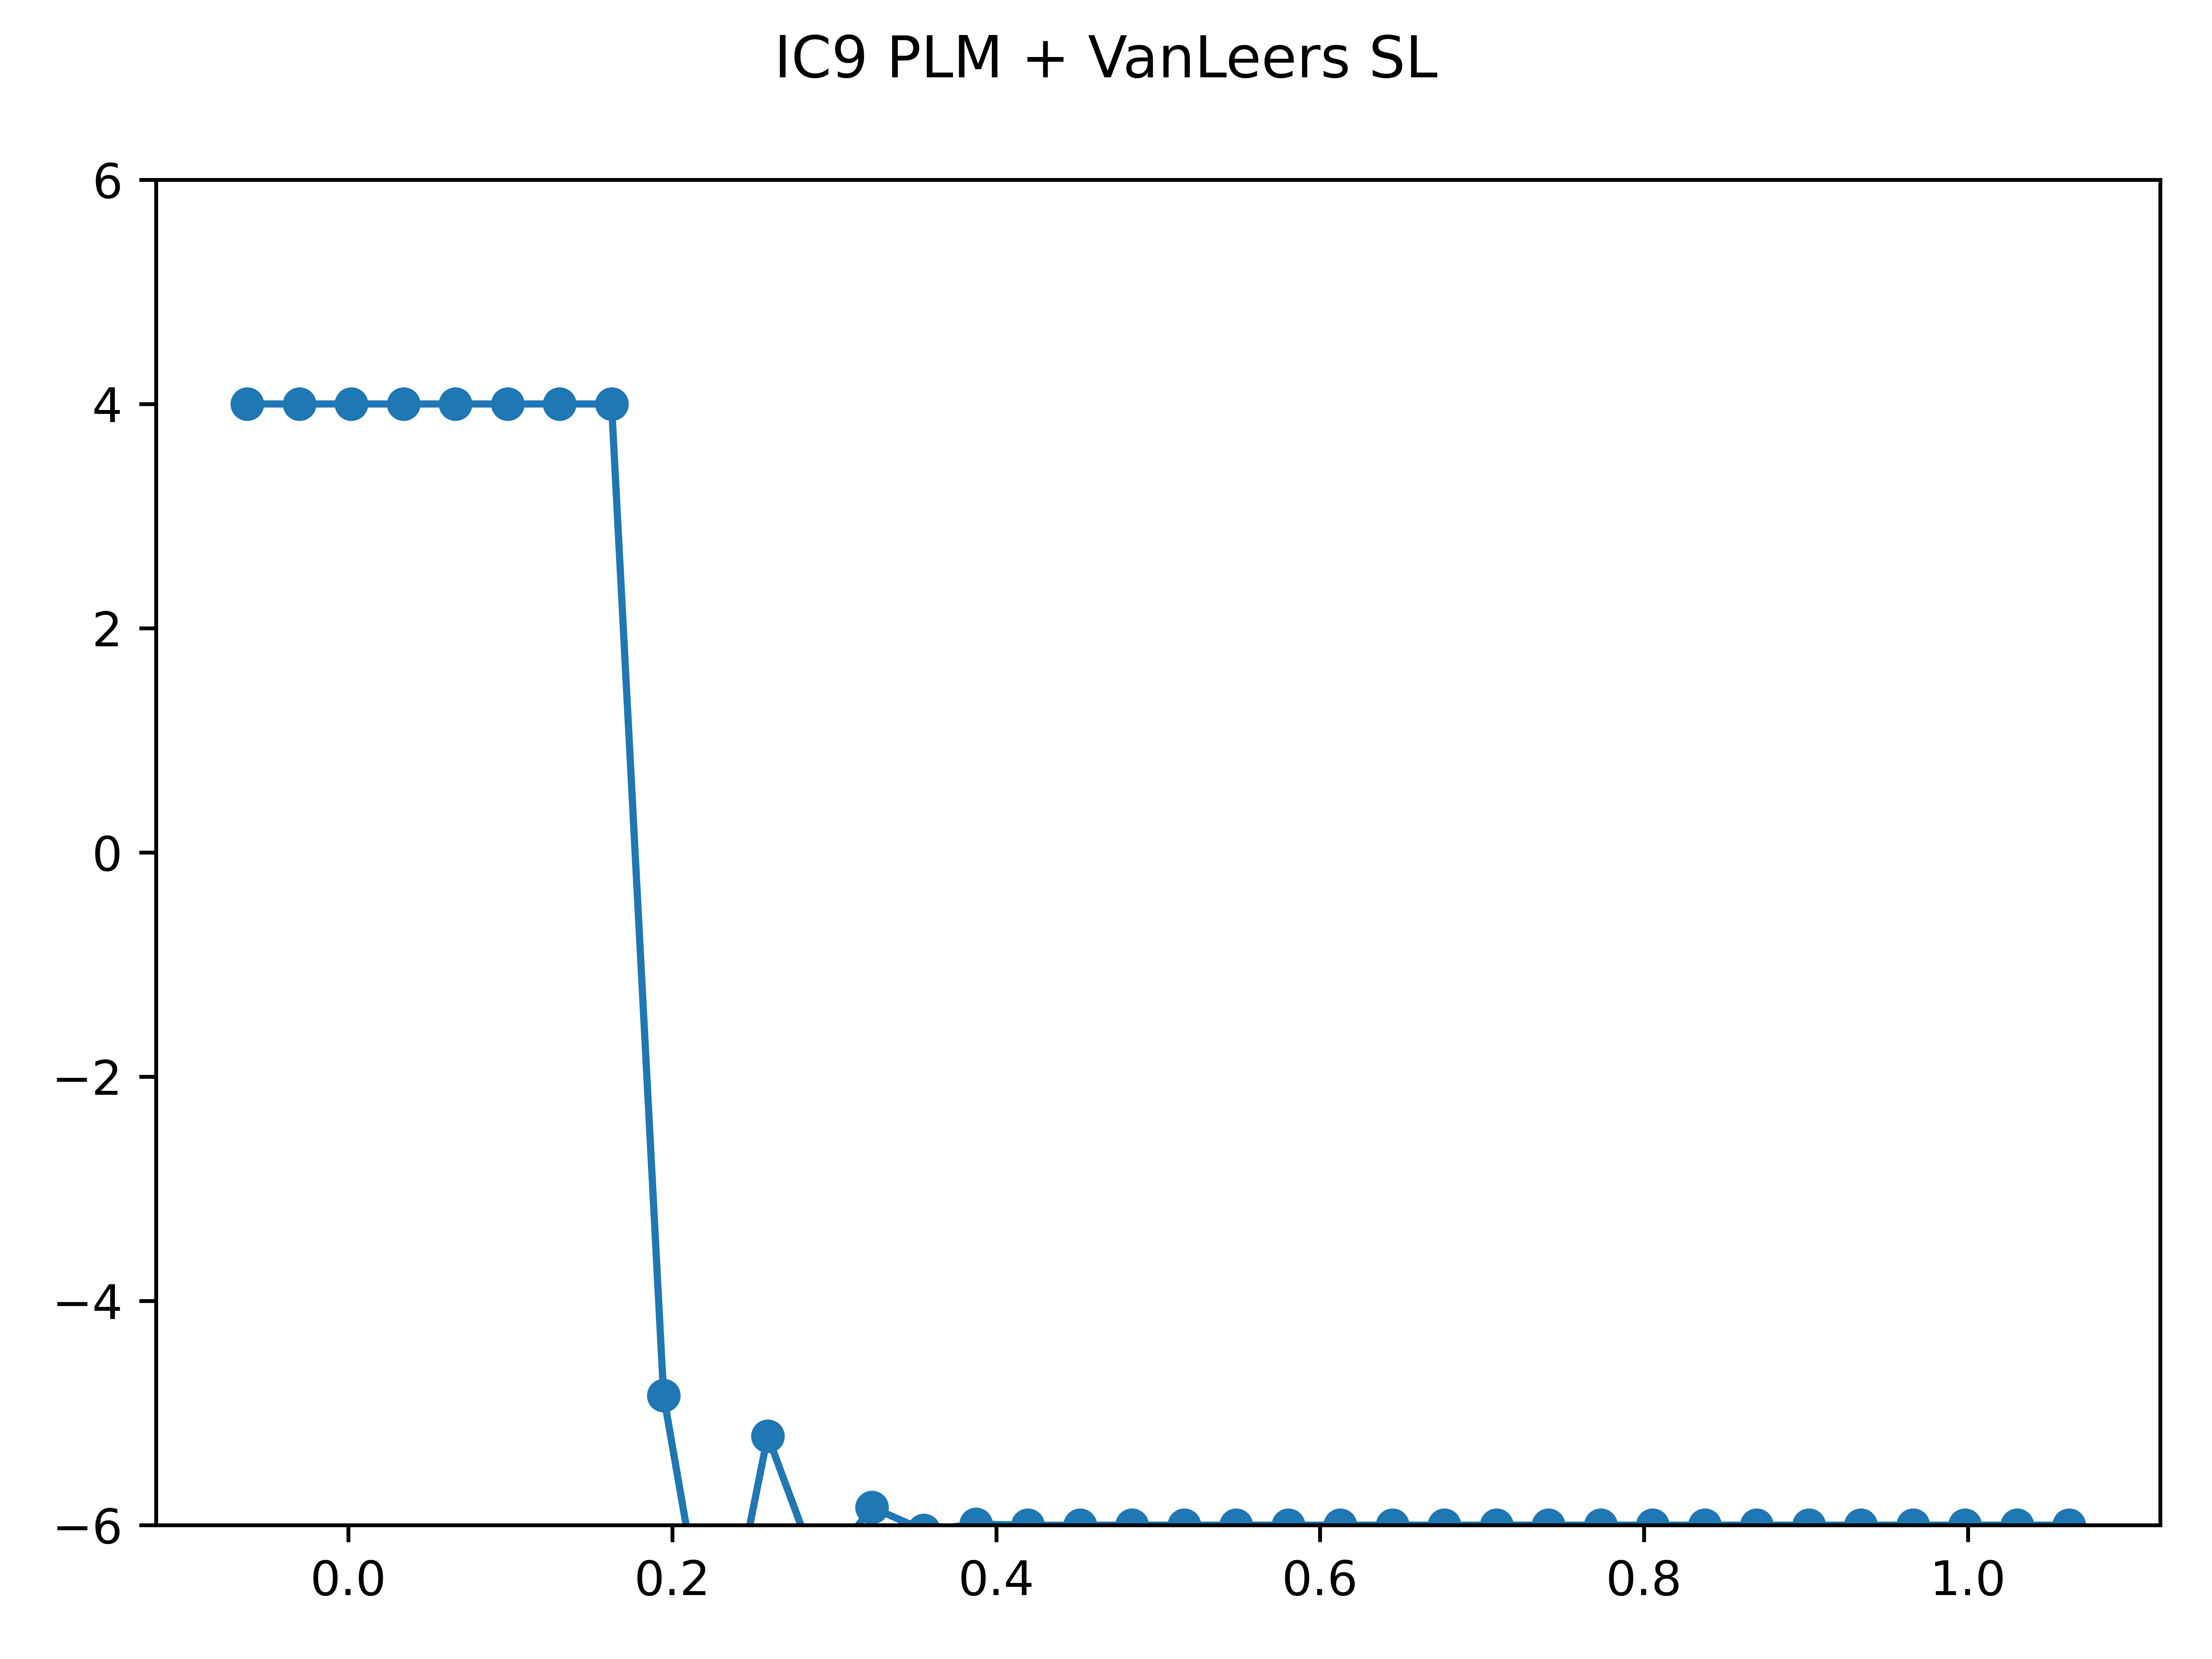
\includegraphics[width=.95\textwidth]{../../code/IC9Methodpv_plot.png}
        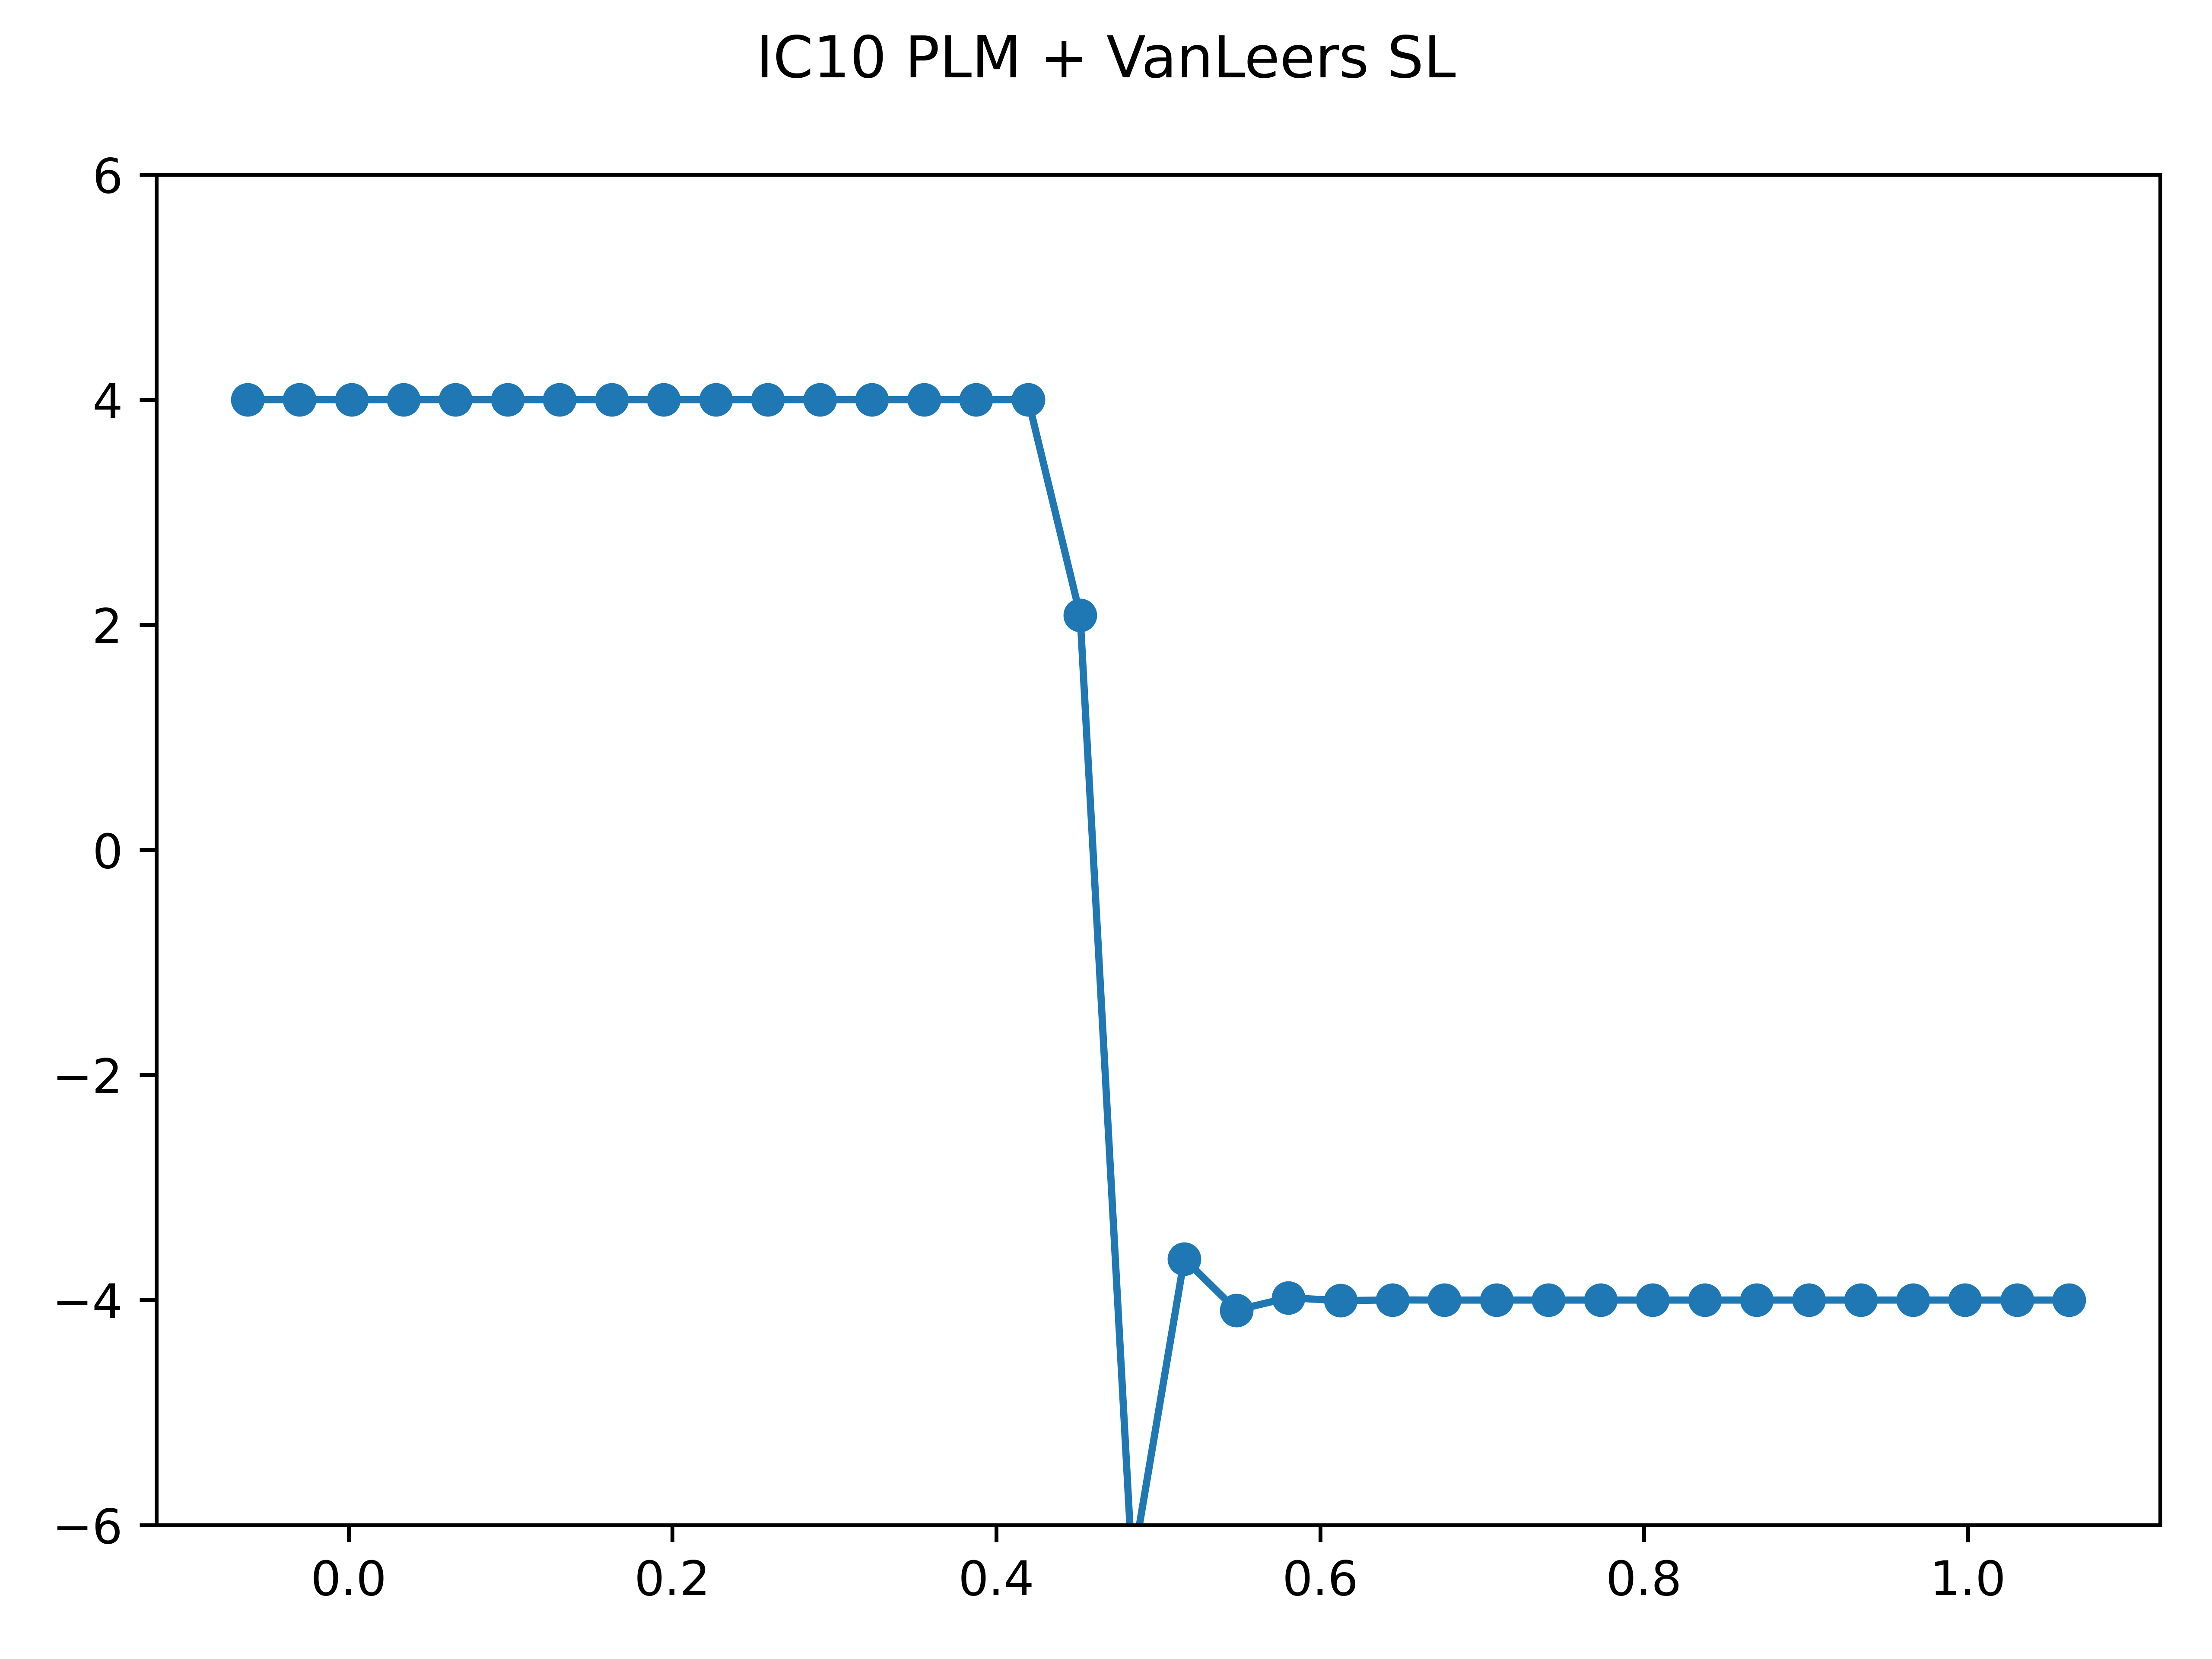
\includegraphics[width=.95\textwidth]{../../code/IC10Methodpv_plot.png}
        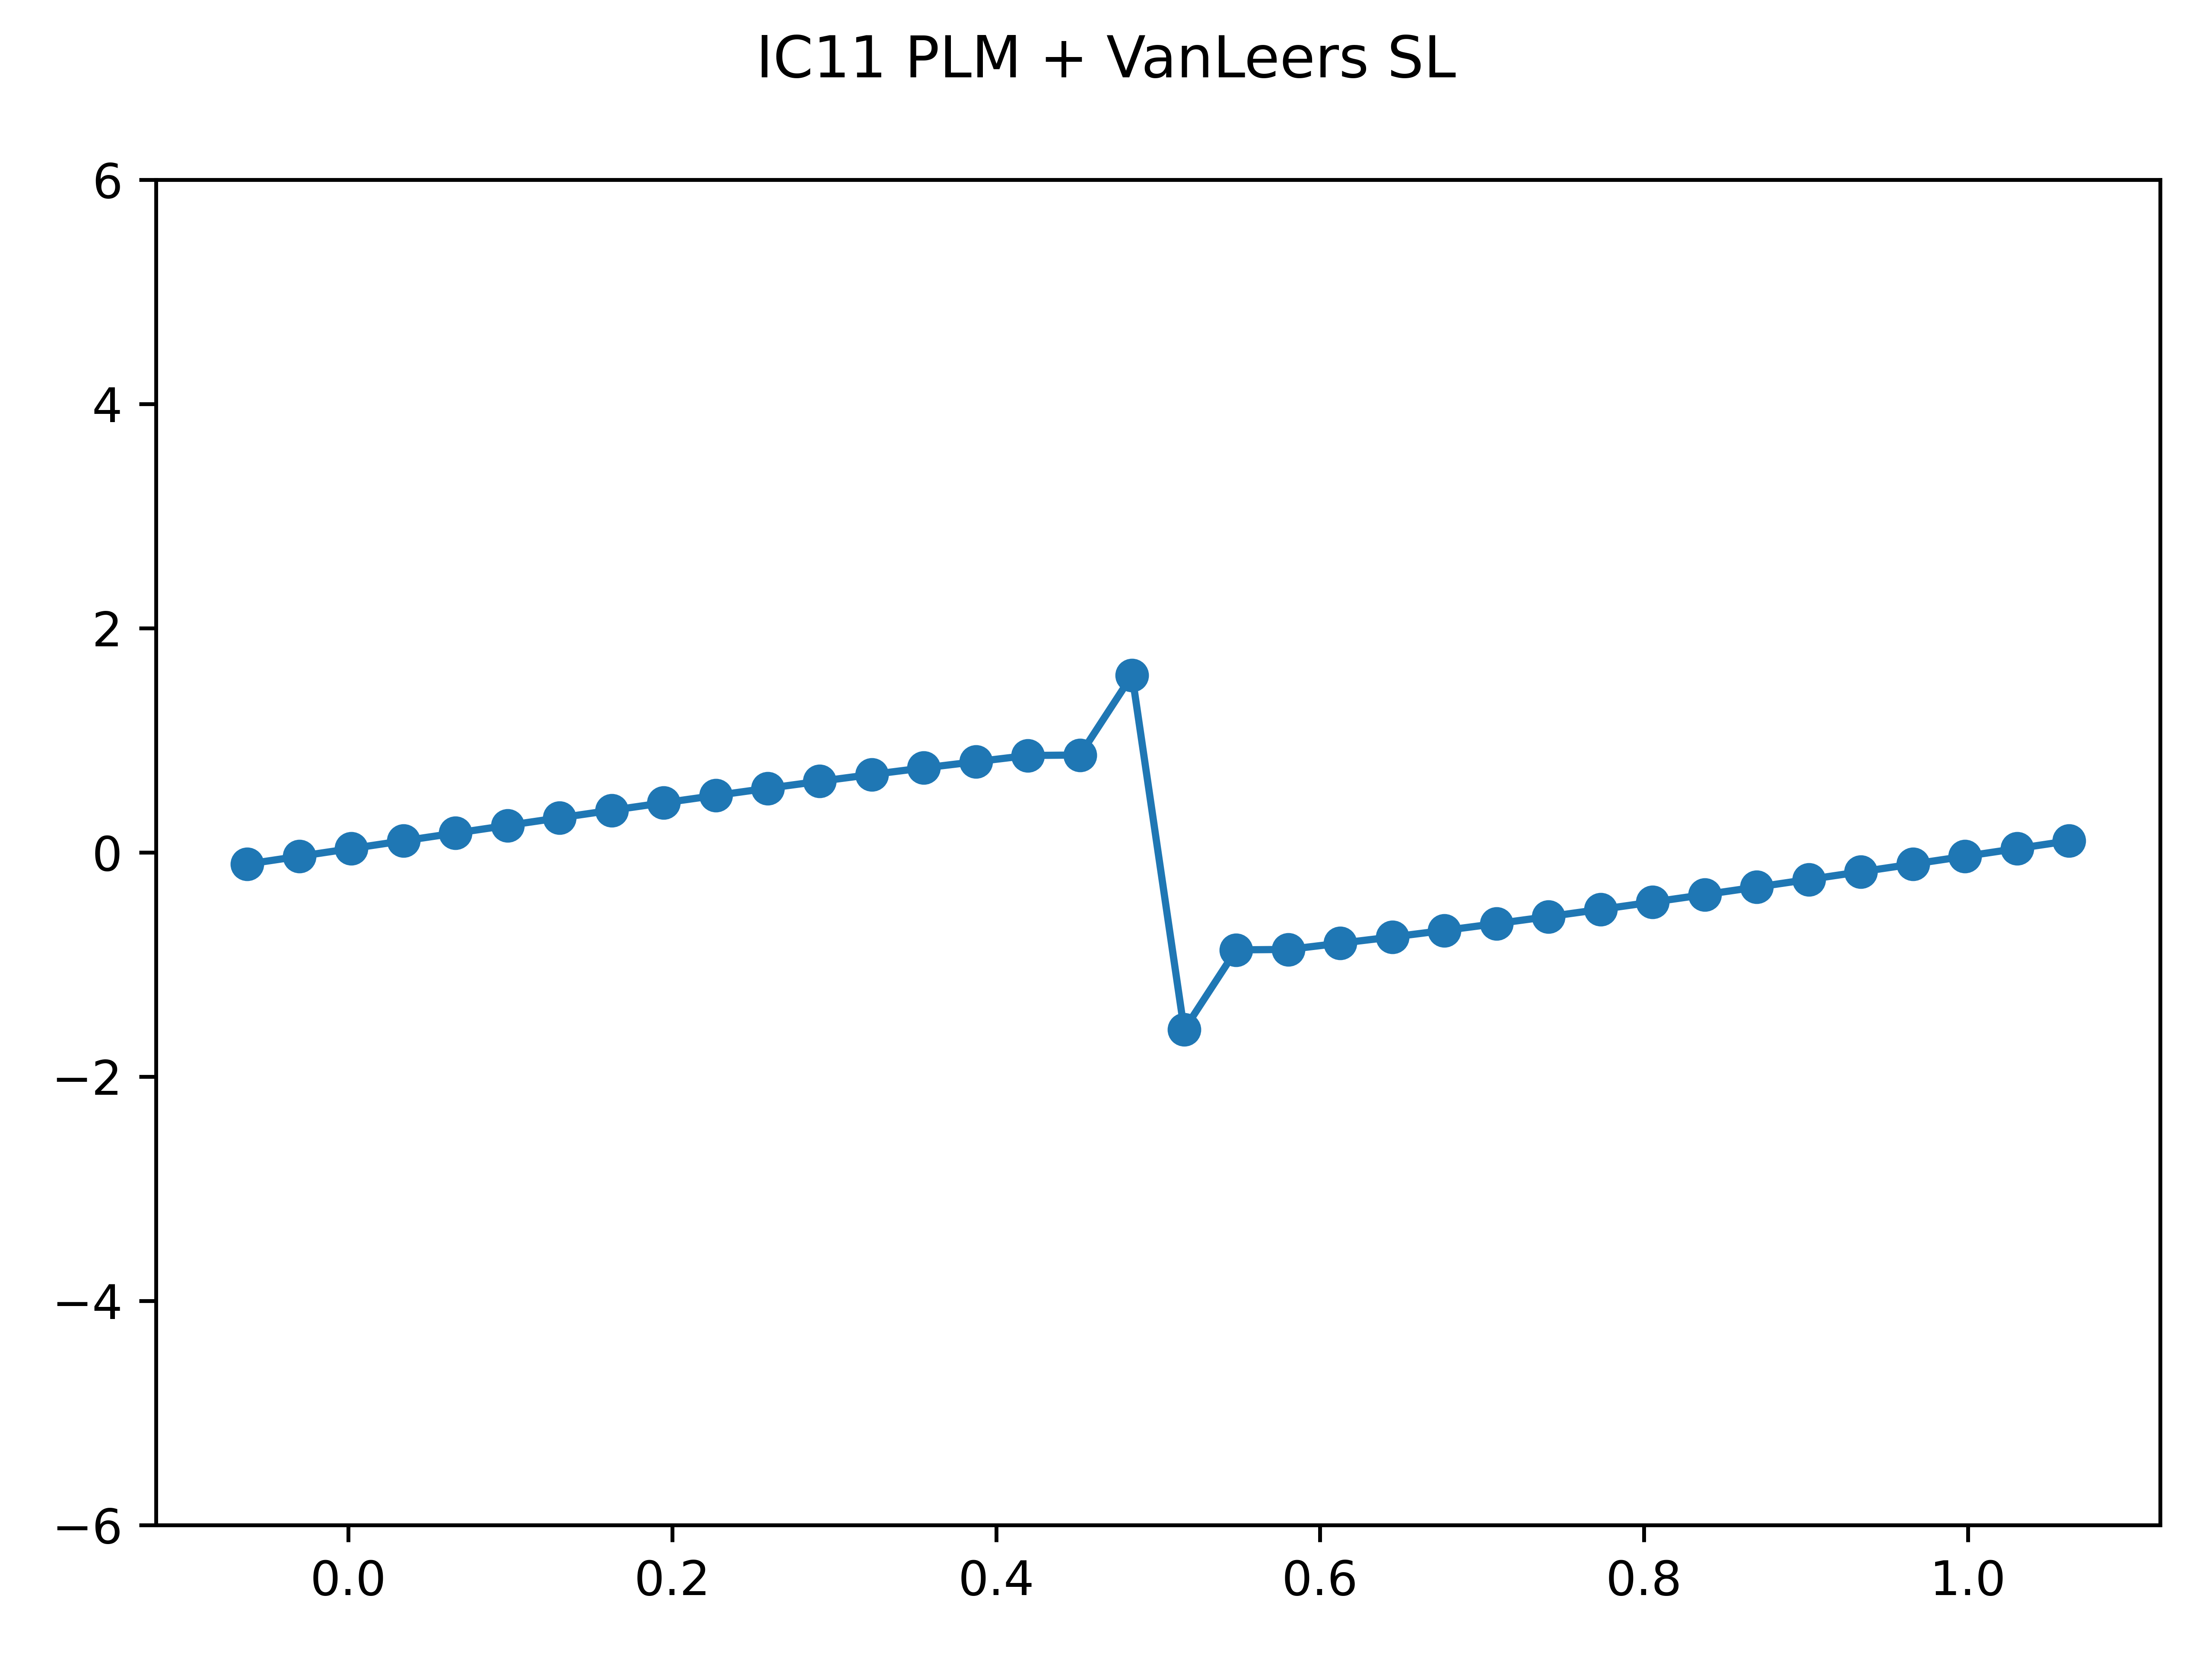
\includegraphics[width=.95\textwidth]{../../code/IC11Methodpv_plot.png}
    \emp
    \caption{Initial Conditions 7-11 (rows) at t=0.3 (or as close as possible before the
    solver crashed for each run). The columns are from left to right, the FOG,
    PLM + Minmod, PLM + MC, and PLM + VanLeers solvers.}
    \label{fig:sol_7_11}
\end{figure}

\section{Part B}

I did two experiments using the data. First, I increased the resolution of the
solutions to $Nx = 100$. Then I ran a simulation with a safety factor of $1.1$
to see if the solution blew up faster. The $Nx = 100$ results are shown in
Figures \ref{fig:hires_sol_1_6} and \ref{fig:hires_sol_7_11}, while the results
for the CFL number being $1.1$ are shown in \ref{fig:unsafe_sol_1_6} and
\ref{fig:unsafe_sol_7_11}. 

Some interesting things that I noticed when running the high resolution ($Nx =
100$) simulations is that most of the shock fronts become steeper due to the
higher resolution. That is, a large part of the reason that they appear to not
be a vertical front is because of discretization size. If we had an infinitely
filled grid, we would probably not see a slope at all! Some other things to
notice is that the numerical errors and oscillations around the discontinuities
appear to change between the low and high resolution runs. They may still be
present but their presentation has changed. 

This is contrasted by the ``unsafe'' (high cfl number) simulations where the
predominant thing to notice is that there are rougher patches visible in the
simulations. For example, in the rarefraction wave initial condition (IC 4) the
edges of the rarefraction fan appear to be jagged. A similar phenomenon can be
seen in the FOG version of IC 7, where on the left of the shock front there
appears to be another jagged bump. Besides this, there are not many differences
between the original cfl = 0.9 and unsafe cfl = 1.1 simulations. 

\begin{figure}[t]
    \bmp{0.25}
        \centering
        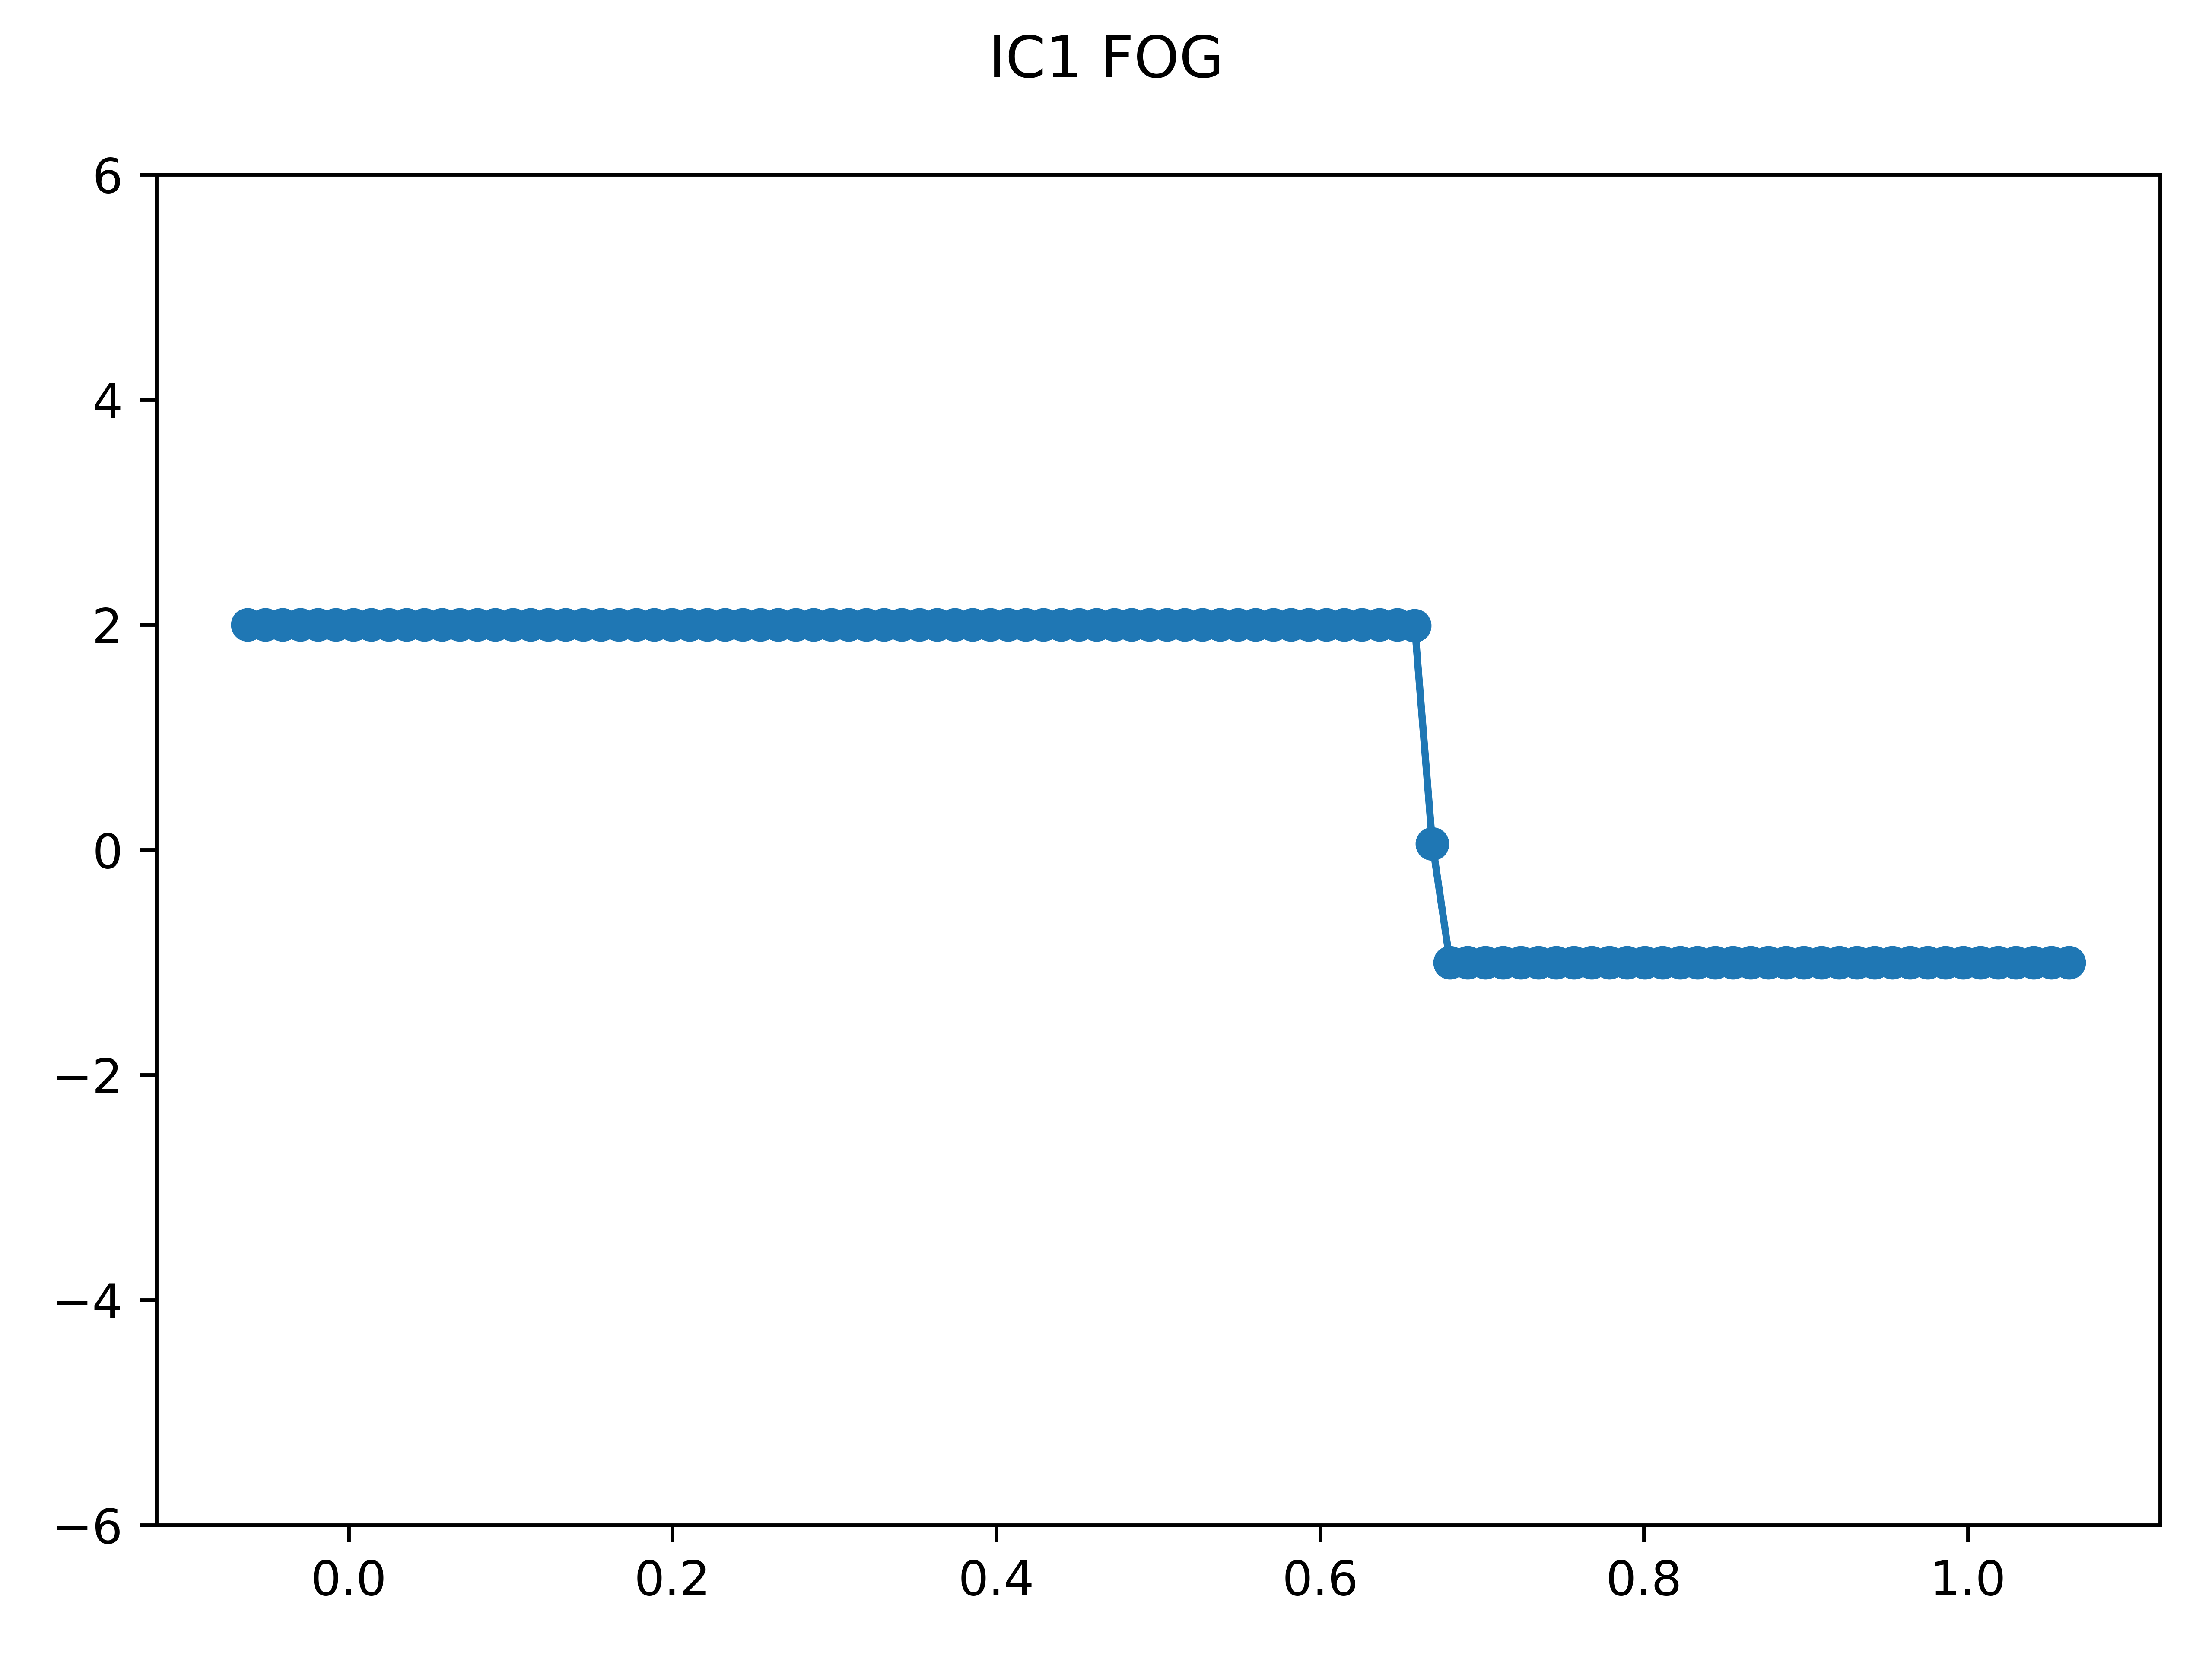
\includegraphics[width=.95\textwidth]{../../code/hires_IC1Methodfu_plot.png}
        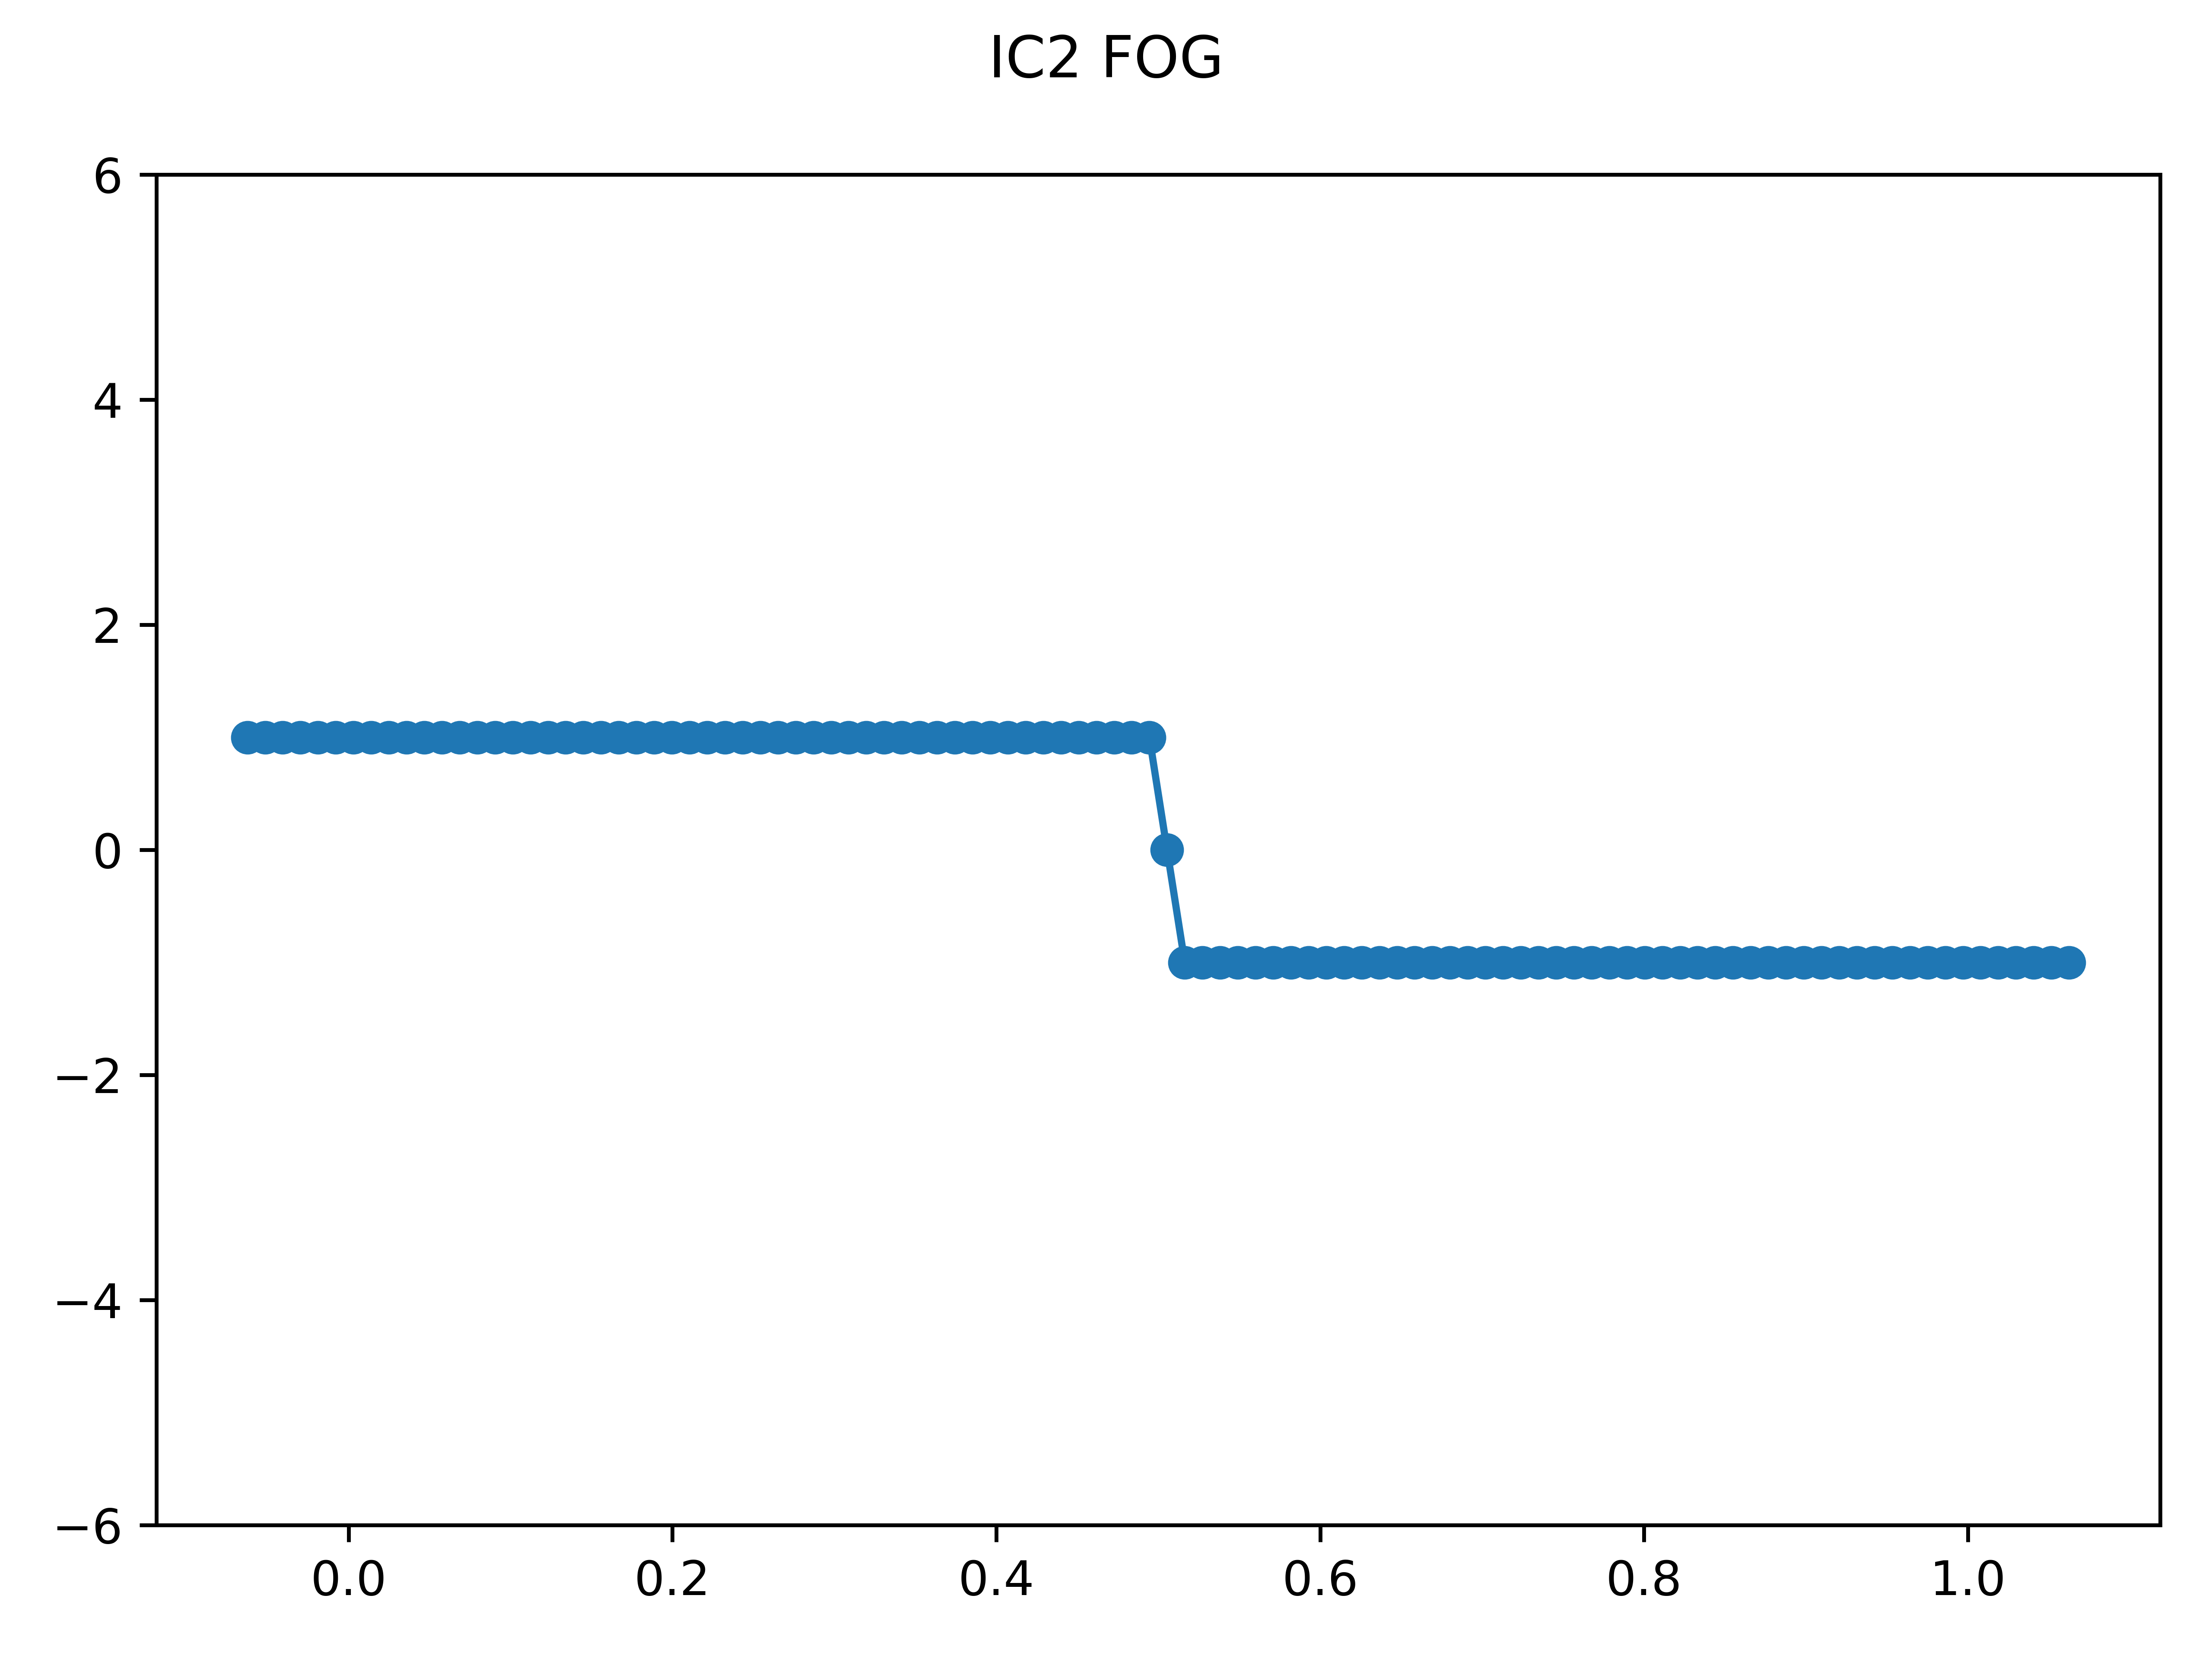
\includegraphics[width=.95\textwidth]{../../code/hires_IC2Methodfu_plot.png}
        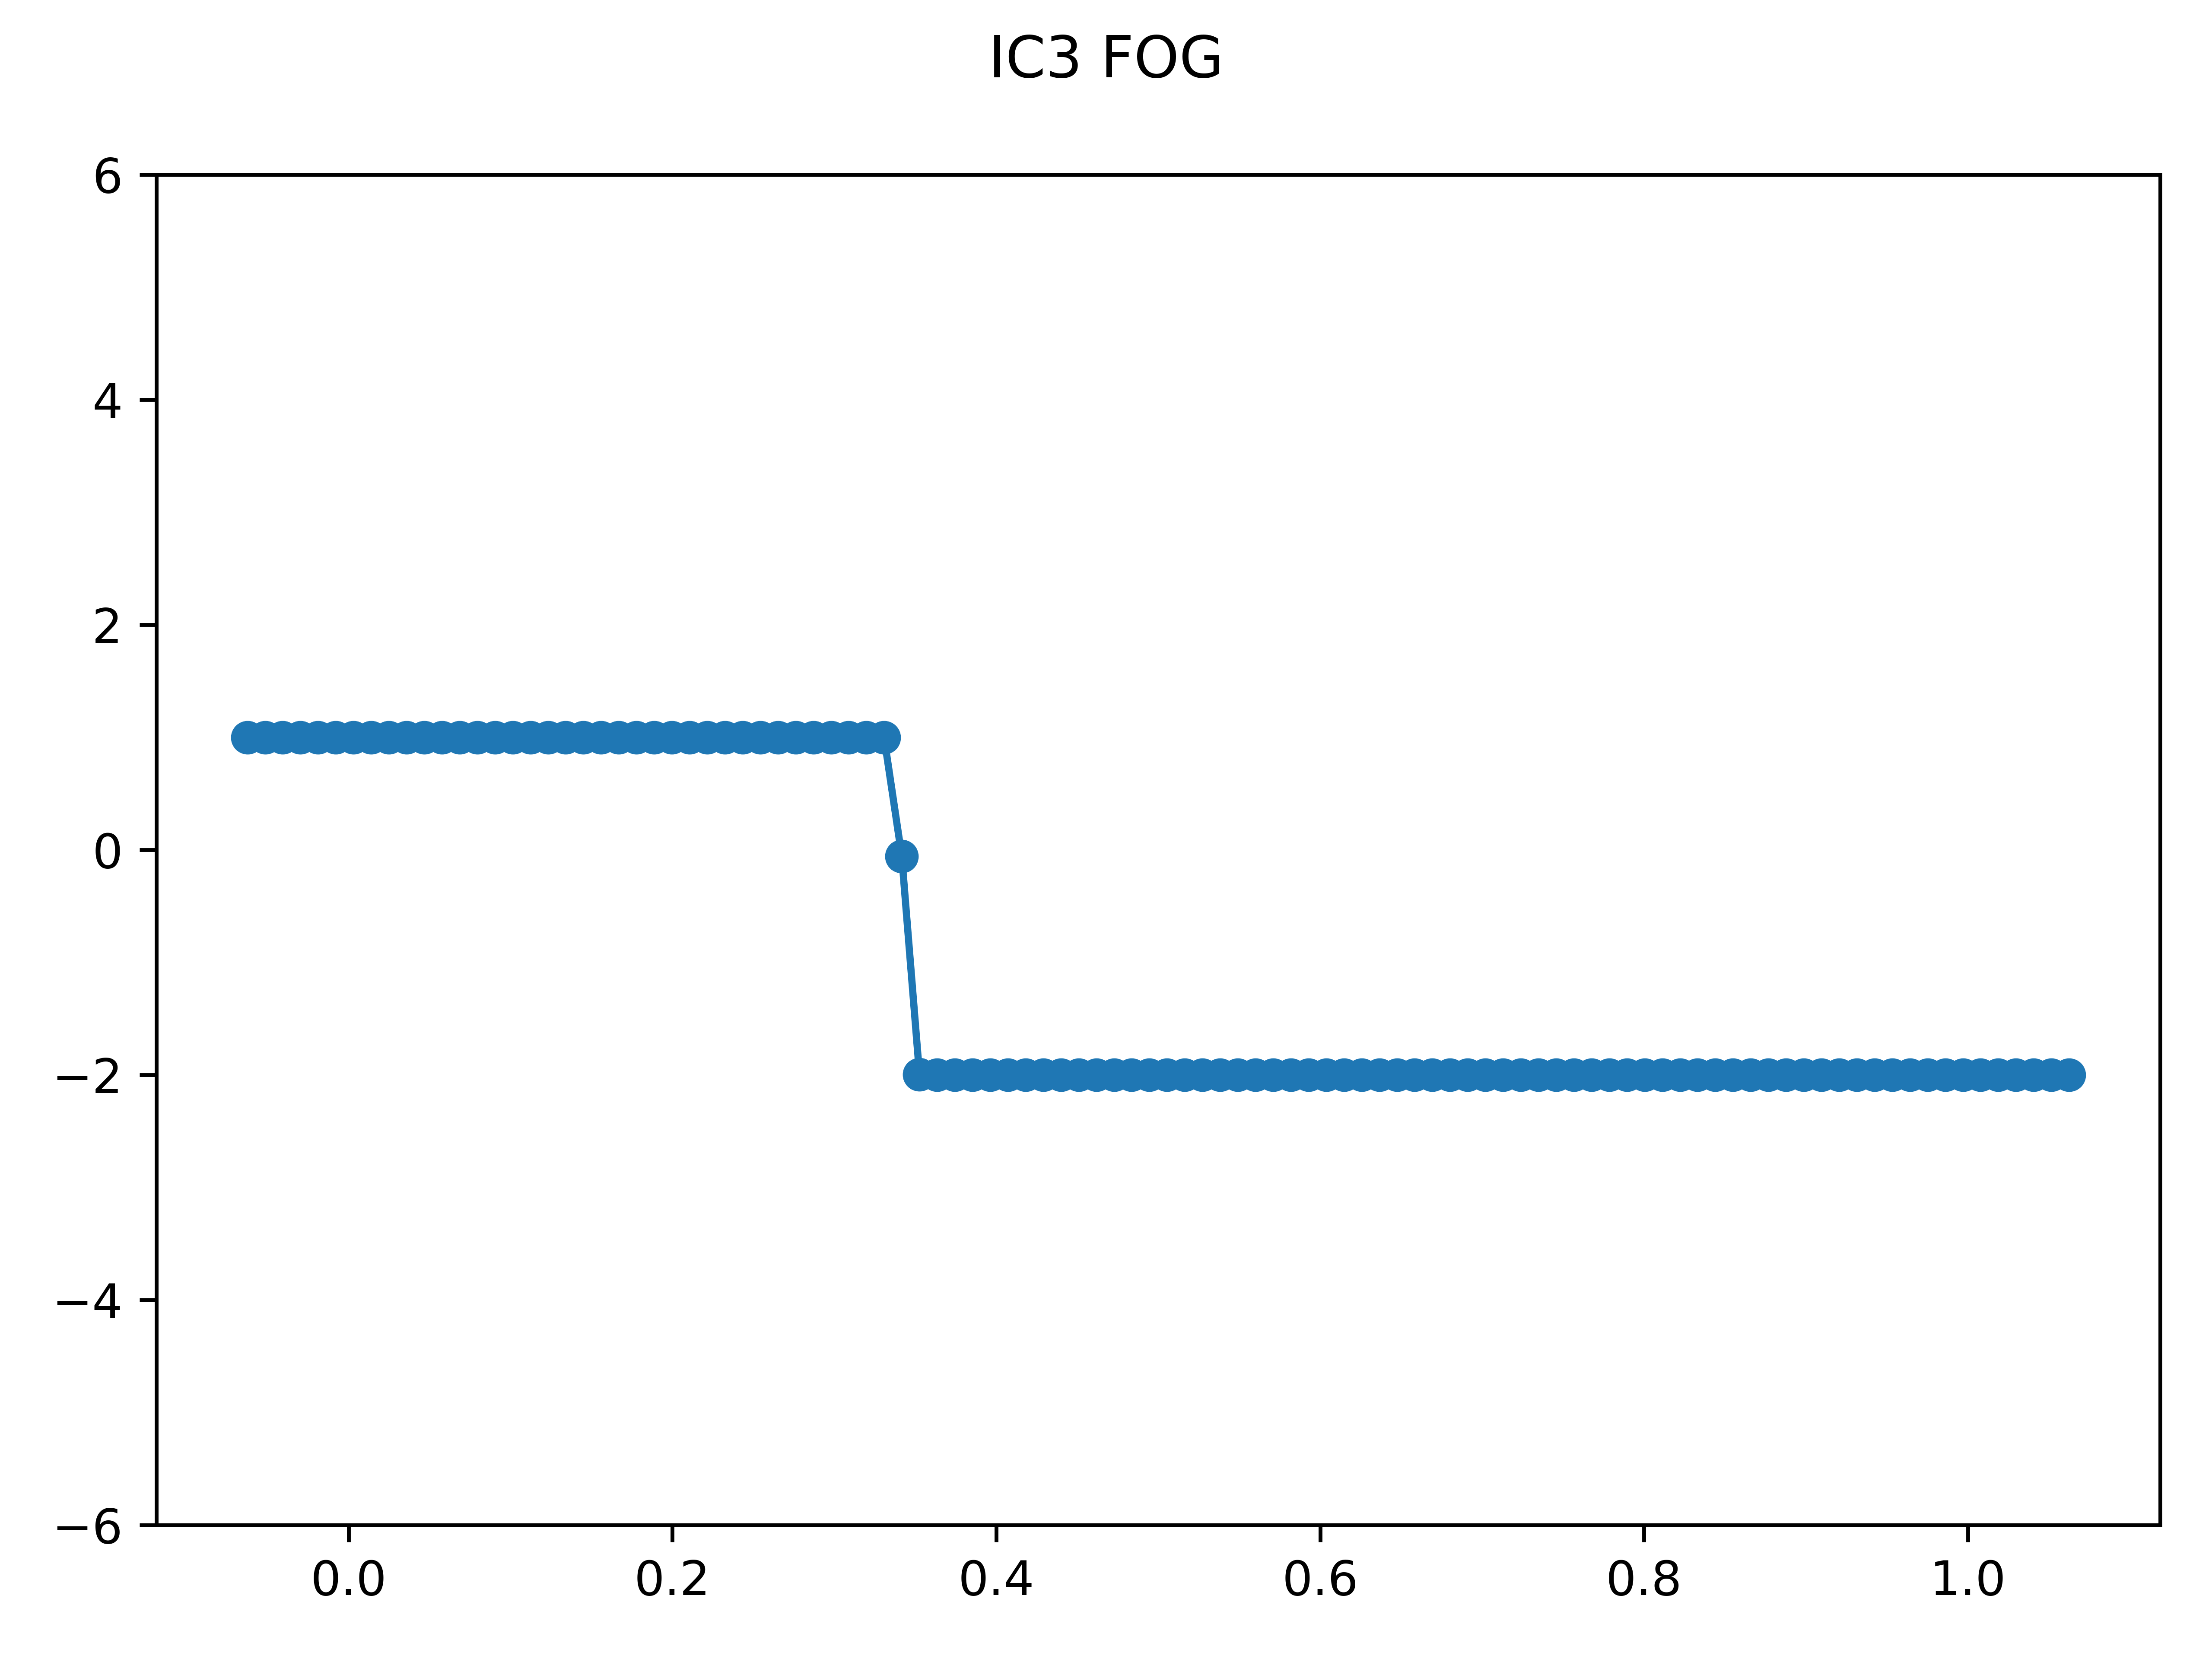
\includegraphics[width=.95\textwidth]{../../code/hires_IC3Methodfu_plot.png}
        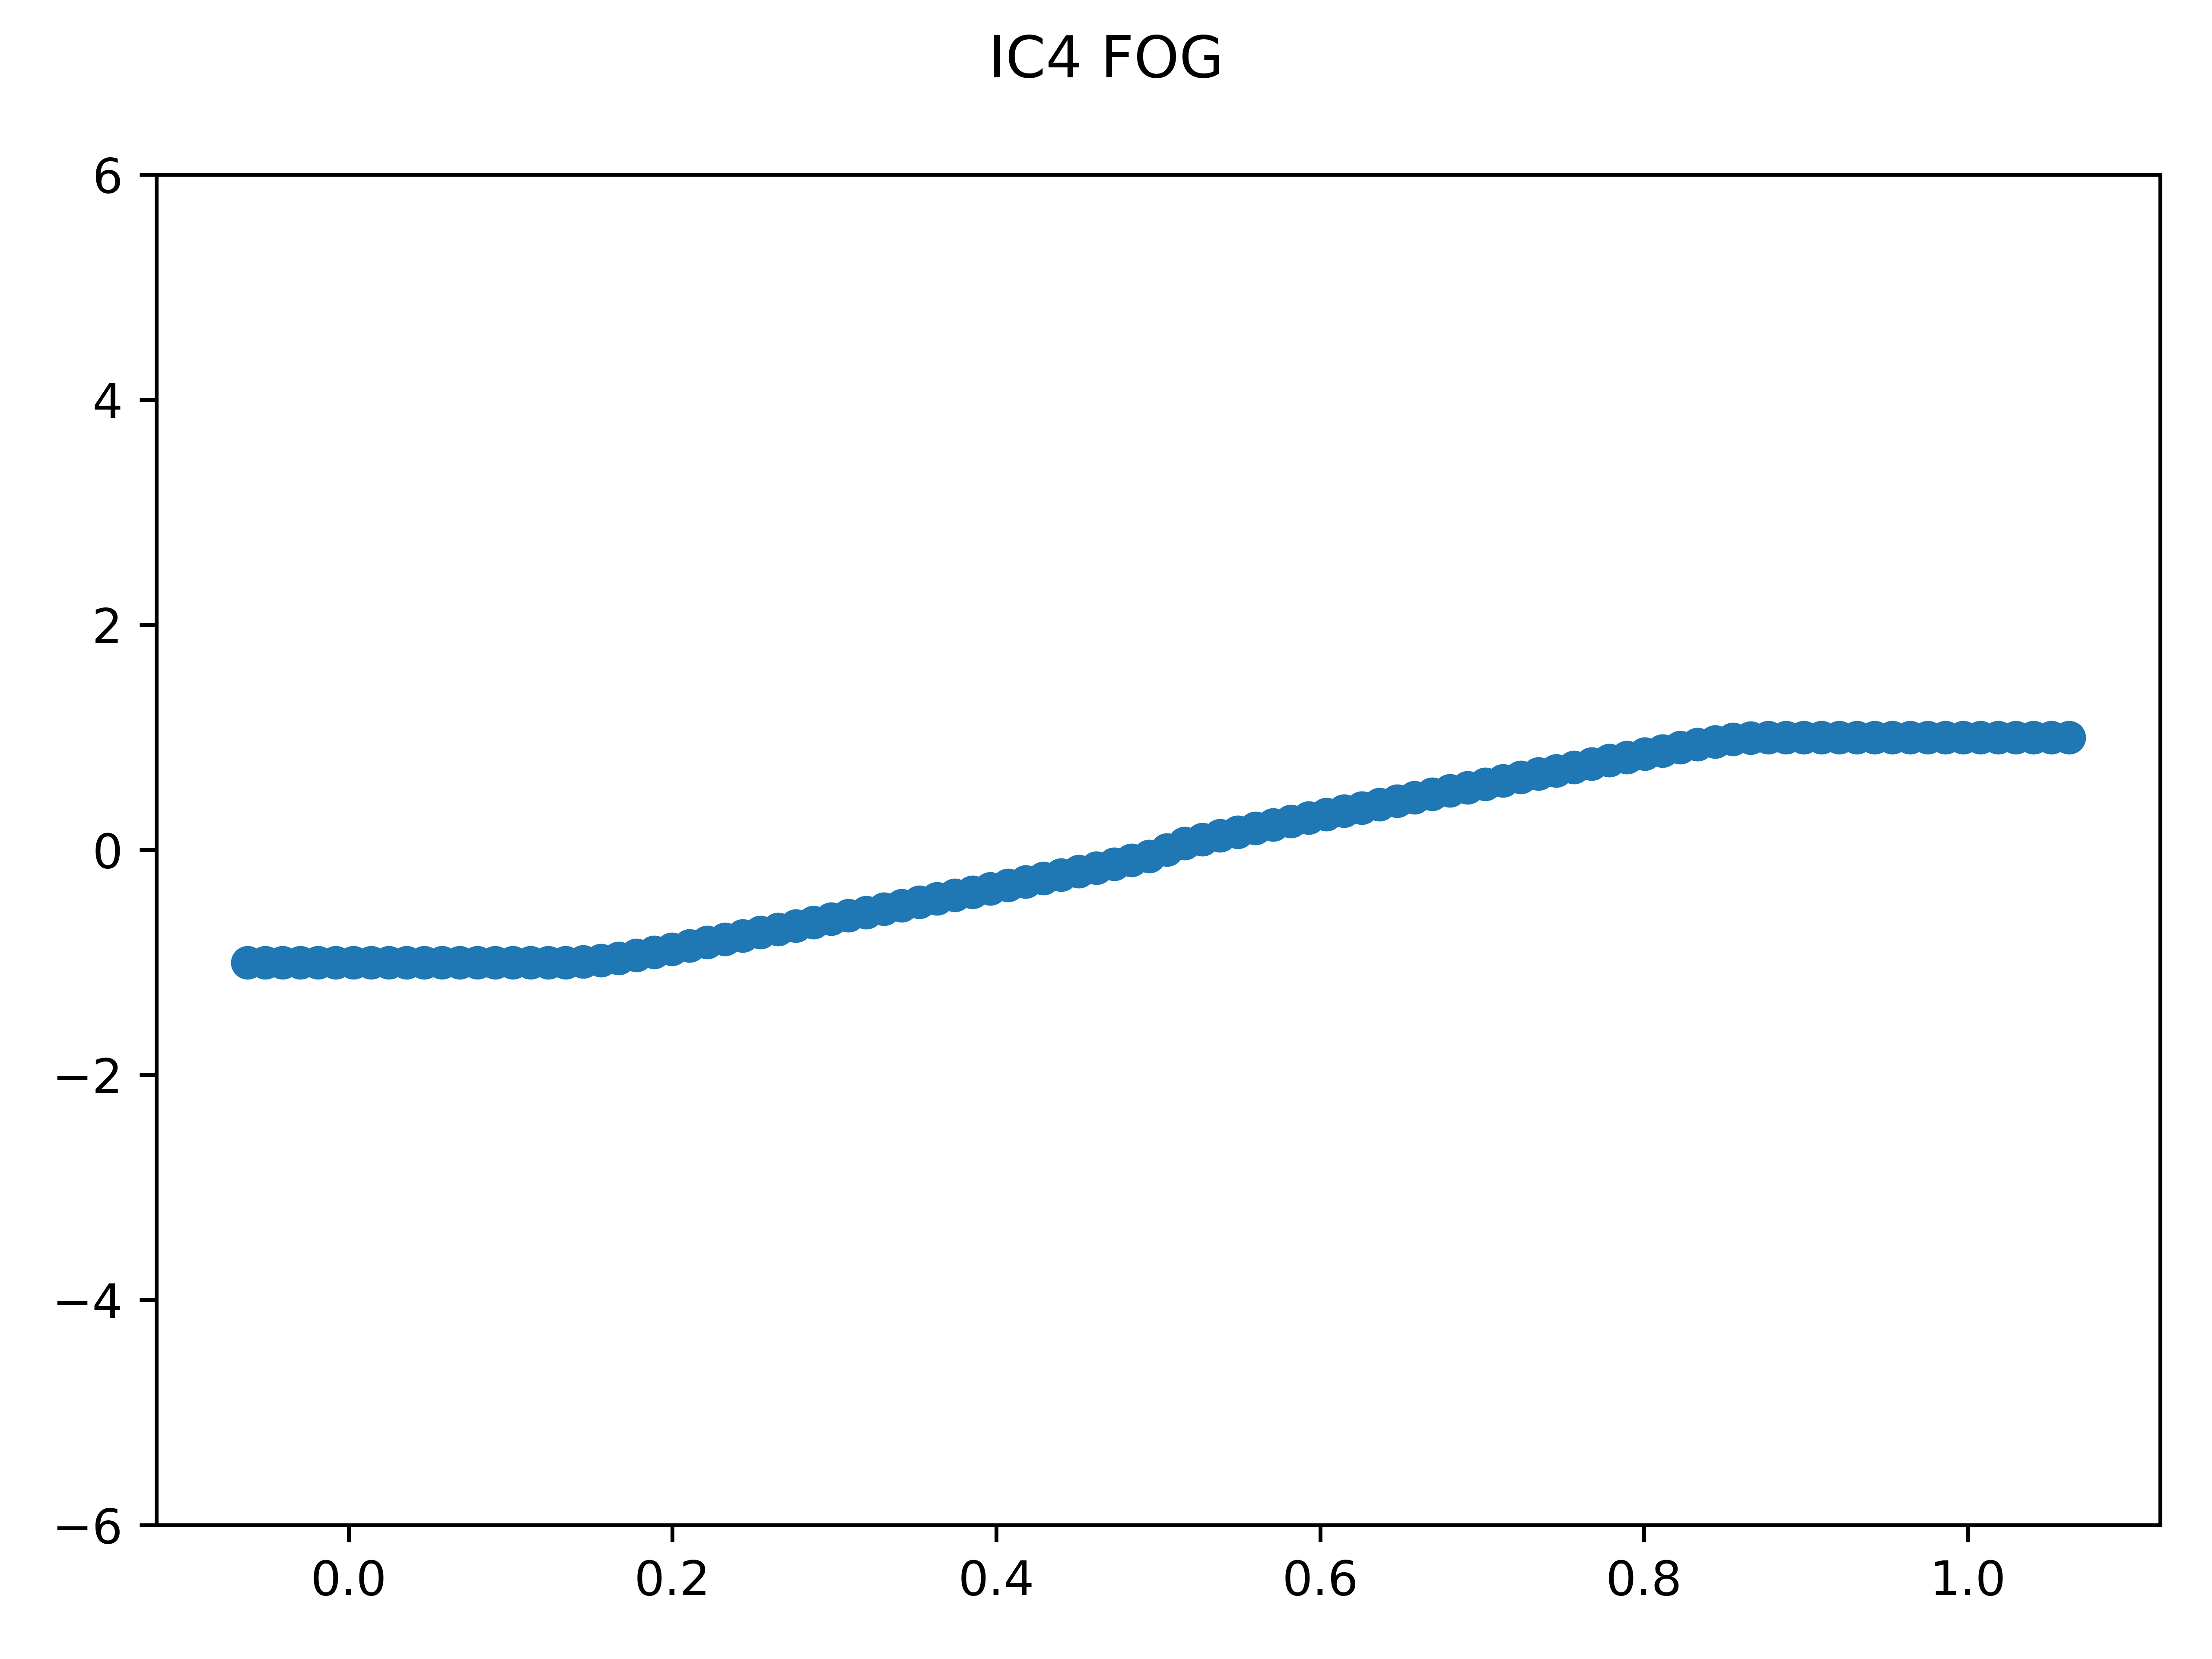
\includegraphics[width=.95\textwidth]{../../code/hires_IC4Methodfu_plot.png}
        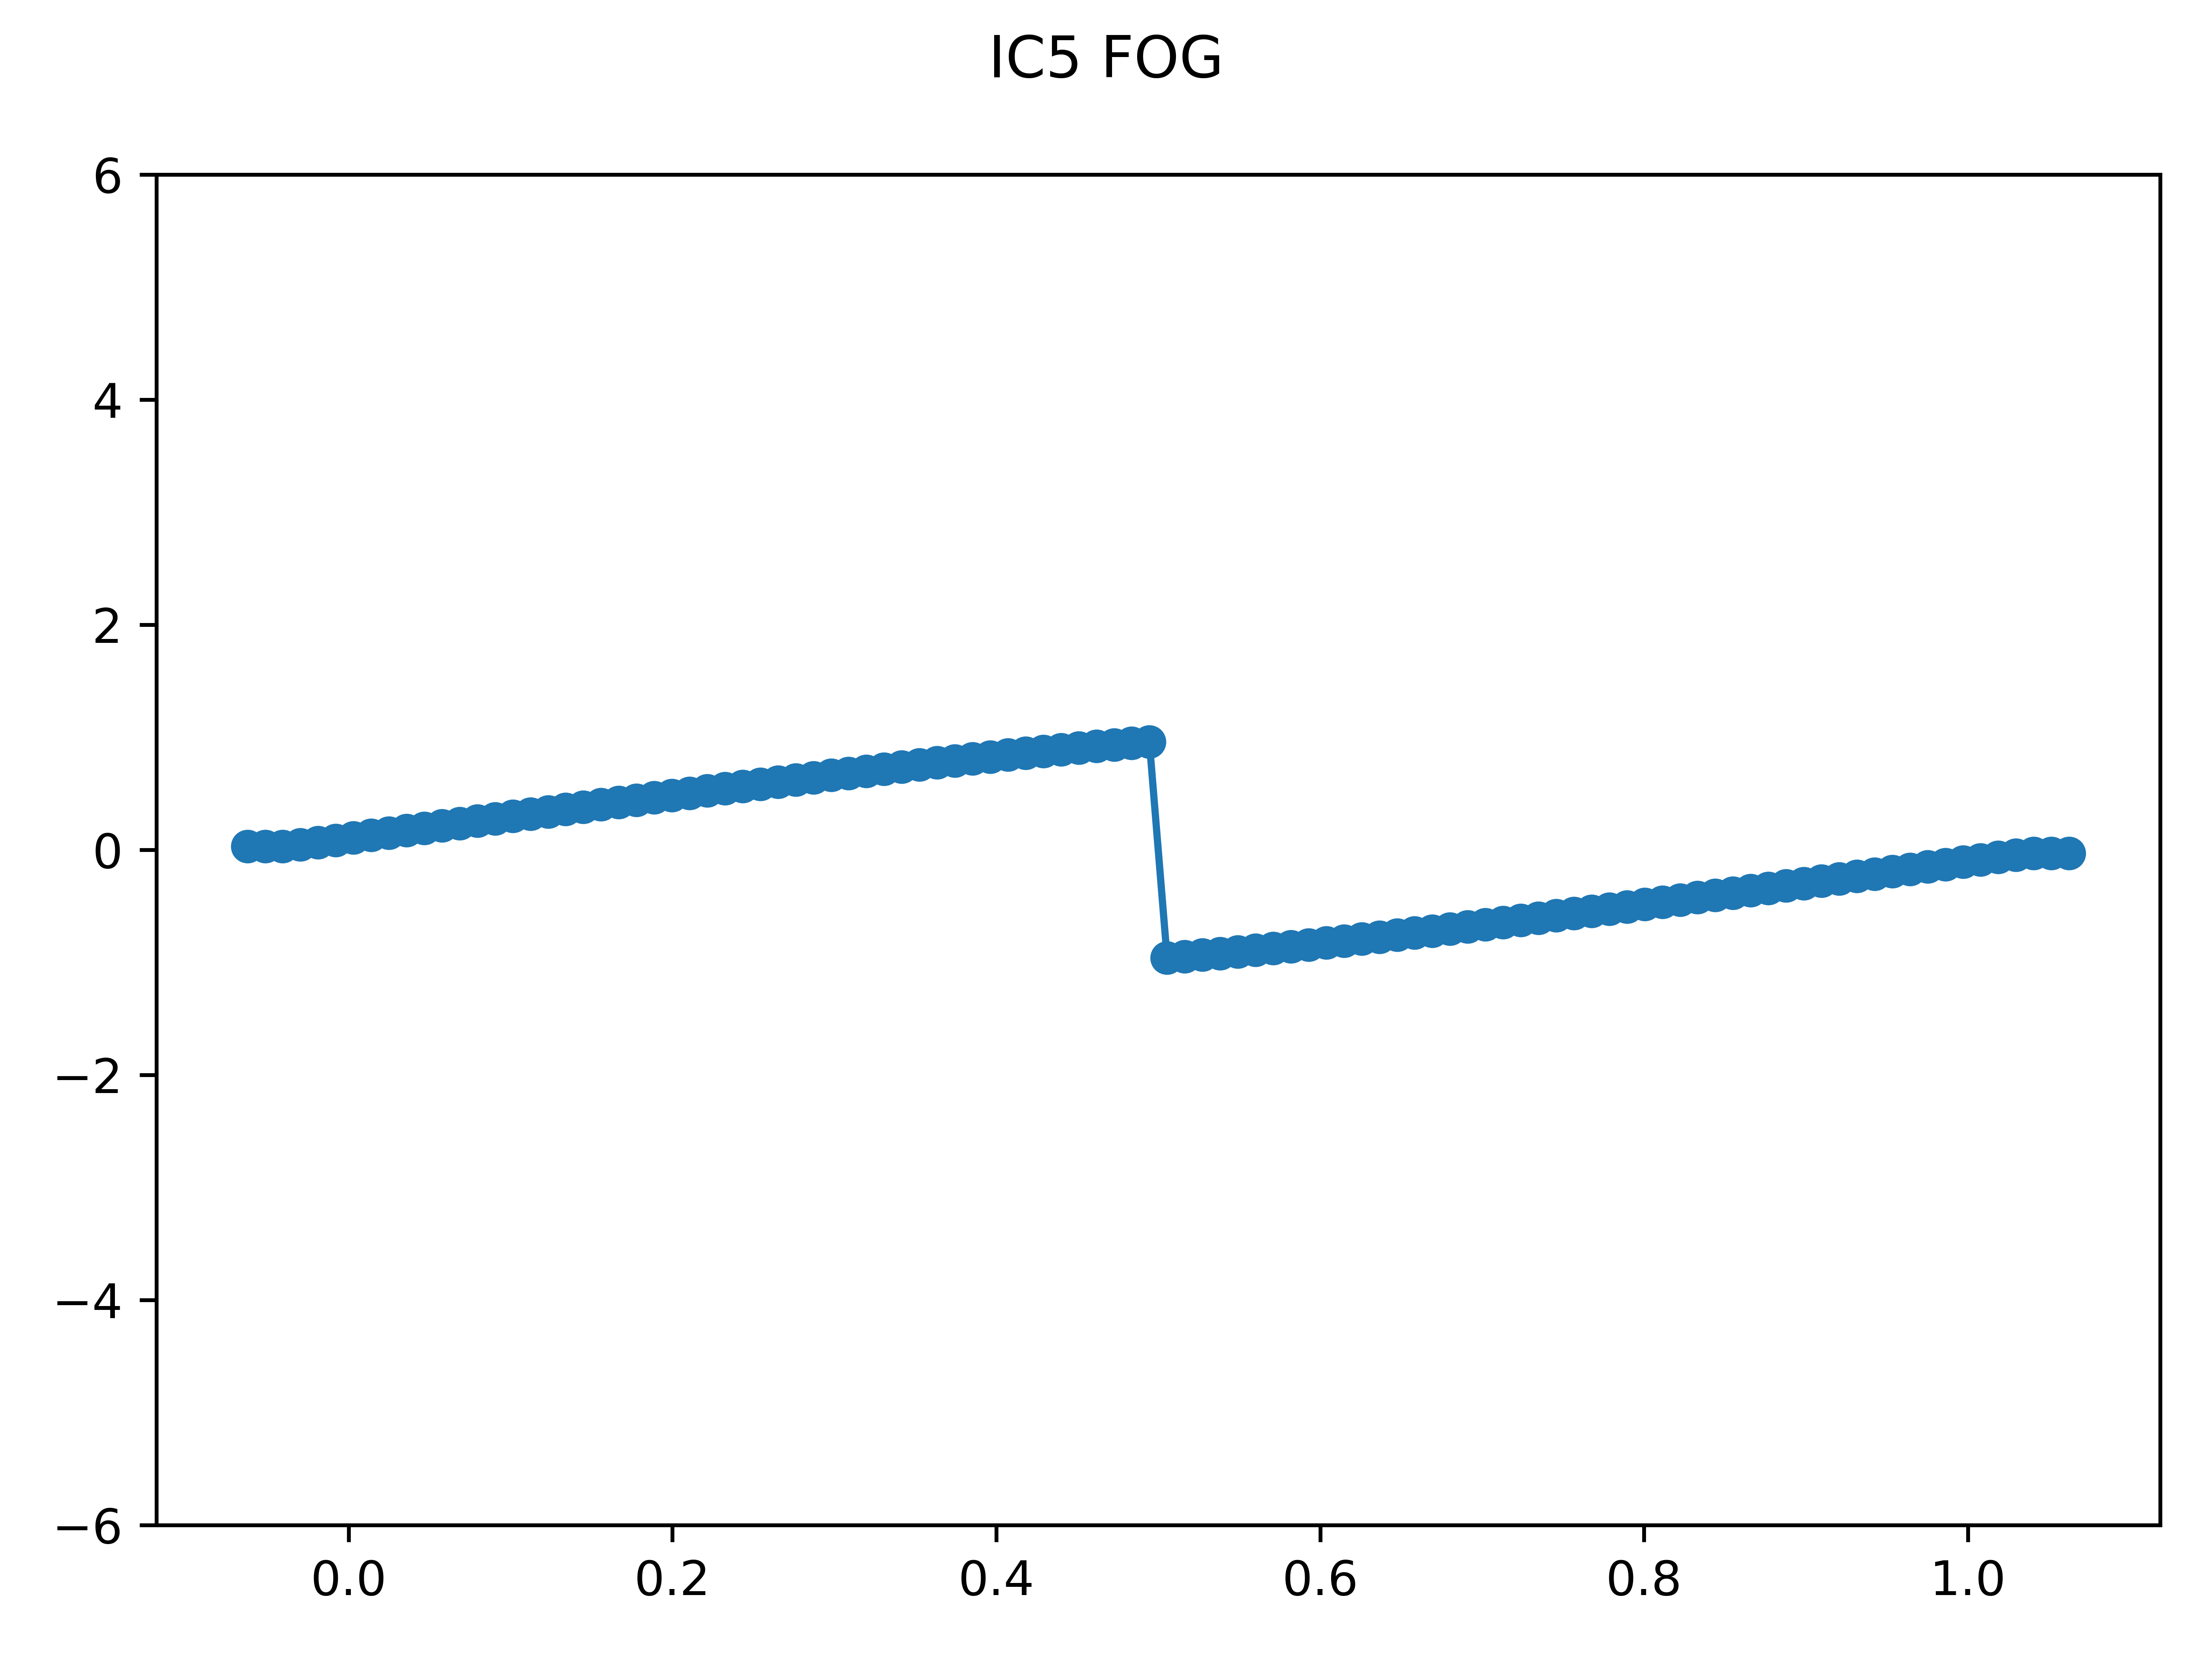
\includegraphics[width=.95\textwidth]{../../code/hires_IC5Methodfu_plot.png}
        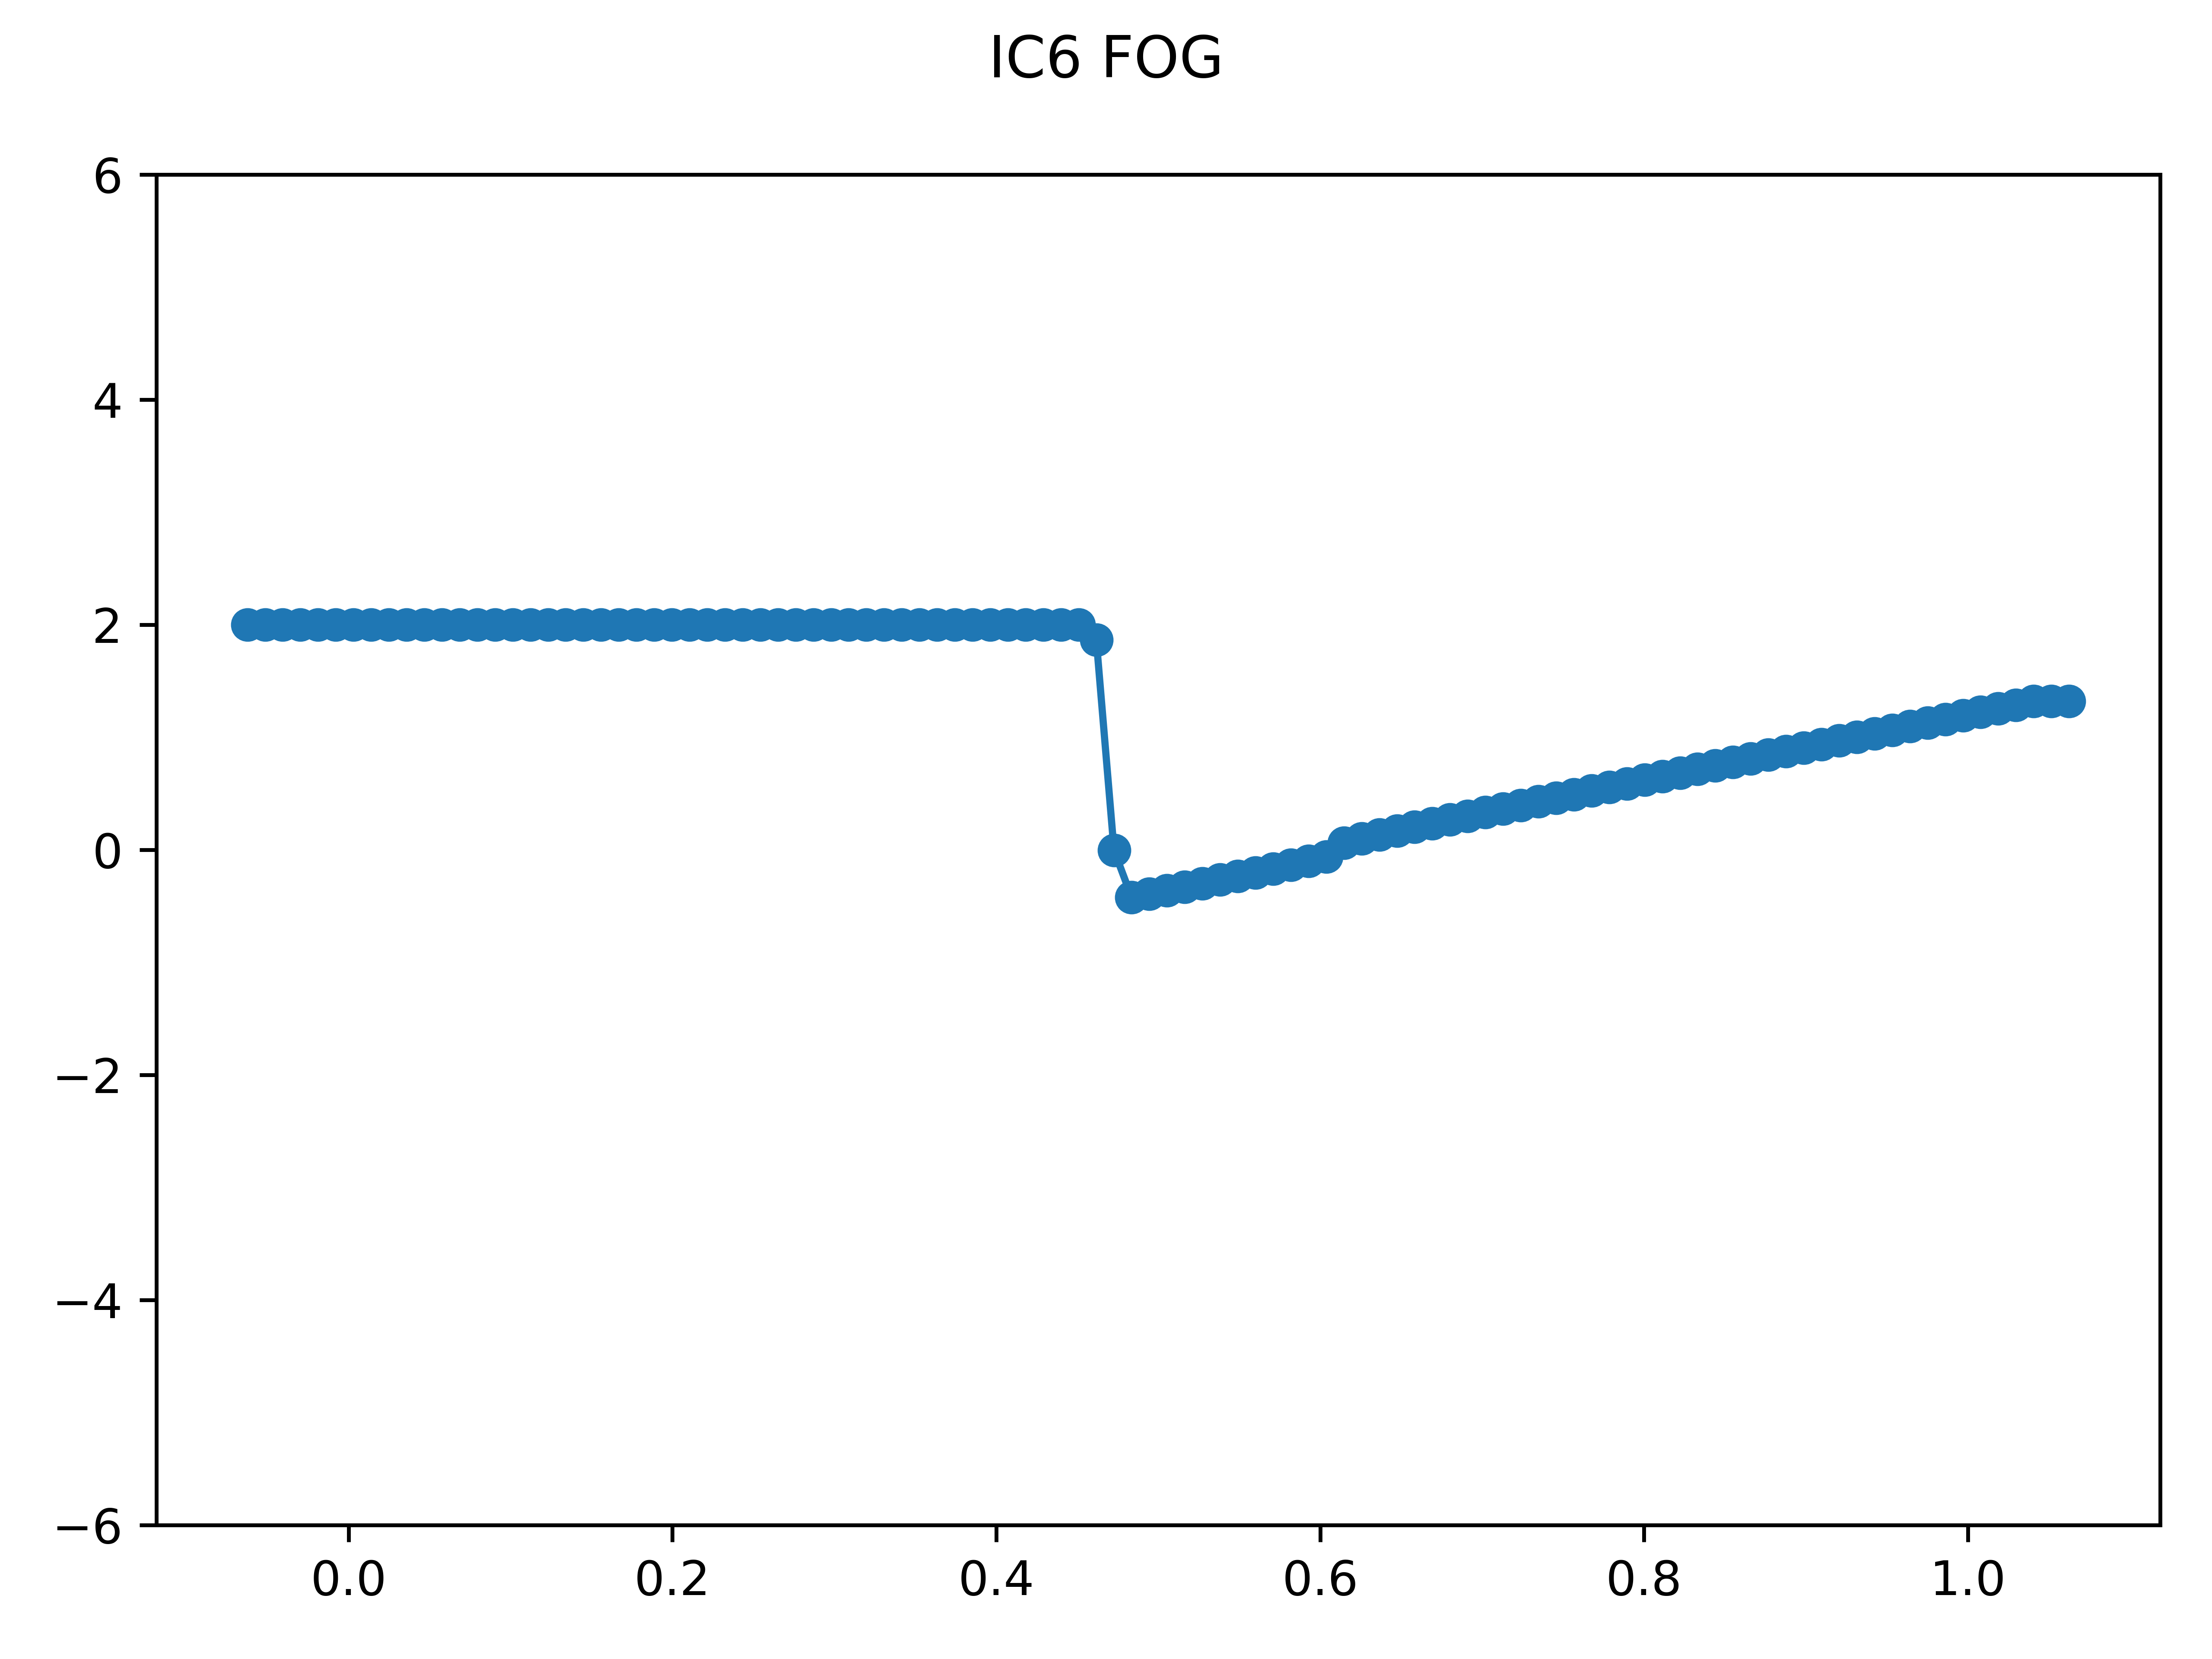
\includegraphics[width=.95\textwidth]{../../code/hires_IC6Methodfu_plot.png}
    \emp
    \bmp{0.25}
        \centering
        \includegraphics[width=.95\textwidth]{../../code/hires_IC1Methodpm_plot.png}
        \includegraphics[width=.95\textwidth]{../../code/hires_IC2Methodpm_plot.png}
        \includegraphics[width=.95\textwidth]{../../code/hires_IC3Methodpm_plot.png}
        \includegraphics[width=.95\textwidth]{../../code/hires_IC4Methodpm_plot.png}
        \includegraphics[width=.95\textwidth]{../../code/hires_IC5Methodpm_plot.png}
        \includegraphics[width=.95\textwidth]{../../code/hires_IC6Methodpm_plot.png}
    \emp
    \bmp{0.25}
        \centering
        \includegraphics[width=.95\textwidth]{../../code/hires_IC1Methodpo_plot.png}
        \includegraphics[width=.95\textwidth]{../../code/hires_IC2Methodpo_plot.png}
        \includegraphics[width=.95\textwidth]{../../code/hires_IC3Methodpo_plot.png}
        \includegraphics[width=.95\textwidth]{../../code/hires_IC4Methodpo_plot.png}
        \includegraphics[width=.95\textwidth]{../../code/hires_IC5Methodpo_plot.png}
        \includegraphics[width=.95\textwidth]{../../code/hires_IC6Methodpo_plot.png}
    \emp
    \bmp{0.25}
        \centering
        \includegraphics[width=.95\textwidth]{../../code/hires_IC1Methodpv_plot.png}
        \includegraphics[width=.95\textwidth]{../../code/hires_IC2Methodpv_plot.png}
        \includegraphics[width=.95\textwidth]{../../code/hires_IC3Methodpv_plot.png}
        \includegraphics[width=.95\textwidth]{../../code/hires_IC4Methodpv_plot.png}
        \includegraphics[width=.95\textwidth]{../../code/hires_IC5Methodpv_plot.png}
        \includegraphics[width=.95\textwidth]{../../code/hires_IC6Methodpv_plot.png}
    \emp
    \caption{Nx = 100, Initial Conditions 1-6 (rows) at t=0.3 (or as close as possible before the
    solver crashed for each run). The columns are from left to right, the FOG,
    PLM + Minmod, PLM + MC, and PLM + VanLeers solvers.}
    \label{fig:hires_sol_1_6}
\end{figure}

\begin{figure}[t]
    \bmp{0.25}
        \centering
        \includegraphics[width=.95\textwidth]{../../code/hires_IC7Methodfu_plot.png}
        \includegraphics[width=.95\textwidth]{../../code/hires_IC8Methodfu_plot.png}
        \includegraphics[width=.95\textwidth]{../../code/hires_IC9Methodfu_plot.png}
        \includegraphics[width=.95\textwidth]{../../code/hires_IC10Methodfu_plot.png}
        \includegraphics[width=.95\textwidth]{../../code/hires_IC11Methodfu_plot.png}
    \emp
    \bmp{0.25}
        \centering
        \includegraphics[width=.95\textwidth]{../../code/hires_IC7Methodpm_plot.png}
        \includegraphics[width=.95\textwidth]{../../code/hires_IC8Methodpm_plot.png}
        \includegraphics[width=.95\textwidth]{../../code/hires_IC9Methodpm_plot.png}
        \includegraphics[width=.95\textwidth]{../../code/hires_IC10Methodpm_plot.png}
        \includegraphics[width=.95\textwidth]{../../code/hires_IC11Methodpm_plot.png}
    \emp
    \bmp{0.25}
        \centering
        \includegraphics[width=.95\textwidth]{../../code/hires_IC7Methodpo_plot.png}
        \includegraphics[width=.95\textwidth]{../../code/hires_IC8Methodpo_plot.png}
        \includegraphics[width=.95\textwidth]{../../code/hires_IC9Methodpo_plot.png}
        \includegraphics[width=.95\textwidth]{../../code/hires_IC10Methodpo_plot.png}
        \includegraphics[width=.95\textwidth]{../../code/hires_IC11Methodpo_plot.png}
    \emp
    \bmp{0.25}
        \centering
        \includegraphics[width=.95\textwidth]{../../code/hires_IC7Methodpv_plot.png}
        \includegraphics[width=.95\textwidth]{../../code/hires_IC8Methodpv_plot.png}
        \includegraphics[width=.95\textwidth]{../../code/hires_IC9Methodpv_plot.png}
        \includegraphics[width=.95\textwidth]{../../code/hires_IC10Methodpv_plot.png}
        \includegraphics[width=.95\textwidth]{../../code/hires_IC11Methodpv_plot.png}
    \emp
    \caption{Nx = 100, Initial Conditions 7-11 (rows) at t=0.3 (or as close as possible before the
    solver crashed for each run). The columns are from left to right, the FOG,
    PLM + Minmod, PLM + MC, and PLM + VanLeers solvers.}
    \label{fig:hires_sol_7_11}
\end{figure}

\begin{figure}[t]
    \bmp{0.25}
        \centering
        \includegraphics[width=.95\textwidth]{../../code/unsafe_IC1Methodfu_plot.png}
        \includegraphics[width=.95\textwidth]{../../code/unsafe_IC2Methodfu_plot.png}
        \includegraphics[width=.95\textwidth]{../../code/unsafe_IC3Methodfu_plot.png}
        \includegraphics[width=.95\textwidth]{../../code/unsafe_IC4Methodfu_plot.png}
        \includegraphics[width=.95\textwidth]{../../code/unsafe_IC5Methodfu_plot.png}
        \includegraphics[width=.95\textwidth]{../../code/unsafe_IC6Methodfu_plot.png}
    \emp
    \bmp{0.25}
        \centering
        \includegraphics[width=.95\textwidth]{../../code/unsafe_IC1Methodpm_plot.png}
        \includegraphics[width=.95\textwidth]{../../code/unsafe_IC2Methodpm_plot.png}
        \includegraphics[width=.95\textwidth]{../../code/unsafe_IC3Methodpm_plot.png}
        \includegraphics[width=.95\textwidth]{../../code/unsafe_IC4Methodpm_plot.png}
        \includegraphics[width=.95\textwidth]{../../code/unsafe_IC5Methodpm_plot.png}
        \includegraphics[width=.95\textwidth]{../../code/unsafe_IC6Methodpm_plot.png}
    \emp
    \bmp{0.25}
        \centering
        \includegraphics[width=.95\textwidth]{../../code/unsafe_IC1Methodpo_plot.png}
        \includegraphics[width=.95\textwidth]{../../code/unsafe_IC2Methodpo_plot.png}
        \includegraphics[width=.95\textwidth]{../../code/unsafe_IC3Methodpo_plot.png}
        \includegraphics[width=.95\textwidth]{../../code/unsafe_IC4Methodpo_plot.png}
        \includegraphics[width=.95\textwidth]{../../code/unsafe_IC5Methodpo_plot.png}
        \includegraphics[width=.95\textwidth]{../../code/unsafe_IC6Methodpo_plot.png}
    \emp
    \bmp{0.25}
        \centering
        \includegraphics[width=.95\textwidth]{../../code/unsafe_IC1Methodpv_plot.png}
        \includegraphics[width=.95\textwidth]{../../code/unsafe_IC2Methodpv_plot.png}
        \includegraphics[width=.95\textwidth]{../../code/unsafe_IC3Methodpv_plot.png}
        \includegraphics[width=.95\textwidth]{../../code/unsafe_IC4Methodpv_plot.png}
        \includegraphics[width=.95\textwidth]{../../code/unsafe_IC5Methodpv_plot.png}
        \includegraphics[width=.95\textwidth]{../../code/unsafe_IC6Methodpv_plot.png}
    \emp
    \caption{CFL = 1.1, Initial Conditions 1-6 (rows) at t=0.3 (or as close as possible before the
    solver crashed for each run). The columns are from left to right, the FOG,
    PLM + Minmod, PLM + MC, and PLM + VanLeers solvers.}
    \label{fig:unsafe_sol_1_6}
\end{figure}

\begin{figure}[t]
    \bmp{0.25}
        \centering
        \includegraphics[width=.95\textwidth]{../../code/unsafe_IC7Methodfu_plot.png}
        \includegraphics[width=.95\textwidth]{../../code/unsafe_IC8Methodfu_plot.png}
        \includegraphics[width=.95\textwidth]{../../code/unsafe_IC9Methodfu_plot.png}
        \includegraphics[width=.95\textwidth]{../../code/unsafe_IC10Methodfu_plot.png}
        \includegraphics[width=.95\textwidth]{../../code/unsafe_IC11Methodfu_plot.png}
    \emp
    \bmp{0.25}
        \centering
        \includegraphics[width=.95\textwidth]{../../code/unsafe_IC7Methodpm_plot.png}
        \includegraphics[width=.95\textwidth]{../../code/unsafe_IC8Methodpm_plot.png}
        \includegraphics[width=.95\textwidth]{../../code/unsafe_IC9Methodpm_plot.png}
        \includegraphics[width=.95\textwidth]{../../code/unsafe_IC10Methodpm_plot.png}
        \includegraphics[width=.95\textwidth]{../../code/unsafe_IC11Methodpm_plot.png}
    \emp
    \bmp{0.25}
        \centering
        \includegraphics[width=.95\textwidth]{../../code/unsafe_IC7Methodpo_plot.png}
        \includegraphics[width=.95\textwidth]{../../code/unsafe_IC8Methodpo_plot.png}
        \includegraphics[width=.95\textwidth]{../../code/unsafe_IC9Methodpo_plot.png}
        \includegraphics[width=.95\textwidth]{../../code/unsafe_IC10Methodpo_plot.png}
        \includegraphics[width=.95\textwidth]{../../code/unsafe_IC11Methodpo_plot.png}
    \emp
    \bmp{0.25}
        \centering
        \includegraphics[width=.95\textwidth]{../../code/unsafe_IC7Methodpv_plot.png}
        \includegraphics[width=.95\textwidth]{../../code/unsafe_IC8Methodpv_plot.png}
        \includegraphics[width=.95\textwidth]{../../code/unsafe_IC9Methodpv_plot.png}
        \includegraphics[width=.95\textwidth]{../../code/unsafe_IC10Methodpv_plot.png}
        \includegraphics[width=.95\textwidth]{../../code/unsafe_IC11Methodpv_plot.png}
    \emp
    \caption{CFL = 1.1, Initial Conditions 7-11 (rows) at t=0.3 (or as close as possible before the
    solver crashed for each run). The columns are from left to right, the FOG,
    PLM + Minmod, PLM + MC, and PLM + VanLeers solvers.}
    \label{fig:unsafe_sol_7_11}
\end{figure}


\section{Part C}

My solution for part C can be best visualized in Figure \ref{fig:pc_sol}. The
shock front developes as it does in IC 11 from the previous examples, but we
also see the shock front advect to the right as the velocity is positive on both
sides of the shock front. In order to design an initial condition which develops
a shock front and propagates to the left we would need to invert the initial
condition (by flipping the sin wave upside down) and then prescribe an initial
velocity which is everywhere negative (by subtracting instead of adding 1.5 to
the sin wave). In these conditions, a shock front would develop and propagate to
the left!

\begin{figure}[t]
    \bmp{0.25}
        \centering
        \includegraphics[width=.95\textwidth]{../../code/pc_IC11Methodfu_plot.png}
    \emp
    \bmp{0.25}
        \centering
        \includegraphics[width=.95\textwidth]{../../code/pc_IC11Methodpm_plot.png}
    \emp
    \bmp{0.25}
        \centering
        \includegraphics[width=.95\textwidth]{../../code/pc_IC11Methodpo_plot.png}
    \emp
    \bmp{0.25}
        \centering
        \includegraphics[width=.95\textwidth]{../../code/pc_IC11Methodpv_plot.png}
    \emp
    \caption{Modified Initial Condition 11 at t=1.5 (or as close as possible before the
    solver crashed for each run). The columns are from left to right, the FOG,
    PLM + Minmod, PLM + MC, and PLM + VanLeers solvers.}
    \label{fig:pc_sol}
\end{figure}


\section{Part D}
    Sorry Dongwook, I haven't done this part yet :'(. 
\end{document}
